% Customizable fields and text areas start with % >> below.
% Lines starting with the comment character (%) are normally removed before release outside the collaboration, but not those comments ending lines

% svn info. These are modified by svn at checkout time.
% The last version of these macros found before the maketitle will be the one on the front page,
% so only the main file is tracked.
% Do not edit by hand!
\RCS$Revision: 252990 $
\RCS$HeadURL: svn+ssh://knash@svn.cern.ch/reps/tdr2/notes/AN-13-004/trunk/AN-13-004.tex $
\RCS$Id: AN-13-004.tex 252990 2014-07-25 15:38:30Z knash $
%%%%%%%%%%%%% local definitions %%%%%%%%%%%%%%%%%%%%%
% This allows for switching between one column and two column (cms@external) layouts
% The widths should  be modified for your particular figures. You'll need additional copies if you have more than one standard figure size.
\newlength\cmsFigWidth
\ifthenelse{\boolean{cms@external}}{\setlength\cmsFigWidth{0.85\columnwidth}}{\setlength\cmsFigWidth{0.4\textwidth}}
\ifthenelse{\boolean{cms@external}}{\providecommand{\cmsLeft}{top}}{\providecommand{\cmsLeft}{left}}
\ifthenelse{\boolean{cms@external}}{\providecommand{\cmsRight}{bottom}}{\providecommand{\cmsRight}{right}}
\newcommand{\wpr}{\ensuremath{\mathrm{W}^\prime}\xspace}
\newcommand{\tbbar}{\ensuremath{{t\overline{b}}}\xspace}
%%%%%%%%%%%%%%%  Title page %%%%%%%%%%%%%%%%%%%%%%%%
\cmsNoteHeader{AN-13-004} % This is over-written in the CMS environment: useful as preprint no. for export versions
% >> Title: please make sure that the non-TeX equivalent is in PDFTitle below
\title{Search for $\mathrm{W'} \to t\bar{b}$ in the all-hadronic final state}


% >> Authors
%Author is always "The CMS Collaboration" for PAS and papers, so author, etc, below will be ignored in those cases
%For multiple affiliations, create an address entry for the combination
%To mark authors as primary, use the \author* form

\address[cern]{CERN}
\address[jhu]{Johns Hopkins University}
\address[ucd]{UC Davis}
\address[sb]{SUNY Buffalo}

\author[cern]{Benedikt Hegner}
\author[jhu]{Guofan Hu}
\author[ucd]{Justin Pilot}
\author[jhu]{Petar Maksimovi\'c}
\author[jhu]{Kevin Nash}
\author[jhu]{Marc Osherson}
\author[sb]{Salvatore Rappoccio}

% >> Date
% The date is in yyyy/mm/dd format. Today has been
% redefined to match, but if the date needs to be fixed, please write it in this fashion.
% For papers and PAS, \today is taken as the date the head file (this one) was last modified according to svn: see the RCS Id string above.
% For the final version it is best to "touch" the head file to make sure it has the latest date.
\date{\today}

% >> Abstract
% Abstract processing:
% 1. **DO NOT use \include or \input** to include the abstract: our abstract extractor will not search through other files than this one.
% 2. **DO NOT use %**                  to comment out sections of the abstract: the extractor will still grab those lines (and they won't be comments any longer!).
% 3. **DO NOT use tex macros**         in the abstract: External TeX parsers used on the abstract don't understand them.

\abstract{
A search for the production of a massive W' boson at an integrated luminosity of 19.7~fb$^{-1}$ is presented.  
We consider the hadronic decay of $W' \to tb$, focusing on events with sufficiently high mass to produce 
highly boosted quarks.  A typical event has a dijet topology composed of a bottom quark and top quark, in which the decay 
products of the latter are merged into a single jet.  Standard model hadronic jet background is reduced by utilizing jet substructure algorithms to identify the top quark jet. 
The production of a right-handed W' with mass below 2.02 TeV is excluded at the 95\% C.L. in the all-hadronic final state.  The increased sensitivity from the combination of the all-hadronic and 
semileptonic final states leads to an exclusion of a right-handed W' with mass below 2.15 TeV at the 95\% C.L. Limits on the W' left- and right-handed couplings are also presented. 
}


% >> PDF Metadata
% Do not comment out the following hypersetup lines (metadata). They will disappear in NODRAFT mode and are needed by CDS.
% Also: make sure that the values of the metadata items are sensible and are in plain text:
% (1) no TeX! -- for \sqrt{s} use sqrt(s) -- this will show with extra quote marks in the draft version but is okay).
% (2) no %.
% (3) No curly braces {}.
\hypersetup{%
pdfauthor={Kevin Nash, Marc Osherson, Salvatore Rappoccio, Petar Maksimovic, Benedikt Hegner, Guofan Hu},%
pdftitle={Search for W prime to tbbar in the all-hadronic final state},%
pdfsubject={CMS},%
pdfkeywords={CMS, physics, software, computing}}

\maketitle %maketitle comes after all the front information has been supplied
% >> Text
%%%%%%%%%%%%%%%%%%%%%%%%%%%%%%%%  Begin text %%%%%%%%%%%%%%%%%%%%%%%%%%%%%
%% **DO NOT REMOVE THE BIBLIOGRAPHY** which is located before the appendix.
%% You can take the text between here and the bibiliography as an example which you should replace with the actual text of your document.
%% If you include other TeX files, be sure to use "\input{filename}" rather than "\input filename".
%% The latter works for you, but our parser looks for the braces and will break when uploading the document.
%%%%%%%%%%%%%%%

\chapter{Introduction to the $\wpr$ Search}

\label{sec:introduction}

Many beyond the Standard Model (BSM) theories predict new massive
gauge bosons.  This note presents a search for a heavy partner of
the Standard Model (SM) W gauge boson, generally referred to as the
$\wpr$ (see Chapter~\ref{sec:BSMtheory}).  
We focus on the $\wpr \to \tbbar$ decay mode motivated by the ability to lower QCD multijet background in this channel when compared to light flavor hadronic decay modes. 


The primary signal under investigation is a $\wpr$ particle in which the interaction with quarks 
is defined by the following Lagrangian,
\begin{eqnarray}
{\cal L} = \frac{V_{q_iq_j}}{2\sqrt{2}} g_w \overline{q}_i\gamma_\mu 
\bigl( a^R_{q_iq_j} (1+{\gamma}^5) + a^L_{q_iq_j}
(1-{\gamma}^5)\bigr) {\wpr} q_j + \mathrm{H.c.} \,,
\label{eqn:Lag}
\end{eqnarray}
This is the most general, lowest-dimensional, model-independent
effective Lagrangian for the $\wpr$ boson.  Here $a_{qi,qj}^{L}$,
$a_{qi,qj}^{R}$ are the left- and right-handed couplings of $\wpr$ to quarks.
For a SM-like $\wpr$, $a_{qi,qj}^{L}$=1, $a_{qi,qj}^{R}=0$.


Searches for a high mass $\wpr$ resonance have been performed at the
Tevatron \cite{PhysRevLett.100.211803,Abazov2011145} and at CMS \cite{CMS-PAS-B2G-12-010,CMS-PAS-EXO-12-060,CMS-PAS-EXO-12-025} and ATLAS \cite{PhysRevLett.109.081801} at the LHC.  
Currently, the most stringent limits on $\wpr$ cross-sections exclude a right-handed $\wpr$ particle with mass below 2.05$~\TeV$ at the 95\% C.L. In this analysis we do not consider \wpr\
  lighter than $\sim$~1.3~$\TeV$ since there are stringent limits on $\wpr$ production at these masses.  

We present a search for $\wpr \to \tbbar$ followed by the
fully hadronic decay chain $\mathrm{t \to W+b}$ followed by $\mathrm{W \to hadrons}$.
This differs from \cite{CMS-PAS-B2G-12-010} since the final state is
comprised of only jets.  In our kinematic regime of interest ($\mathrm{M_{\wpr}
\gtrsim 1.3~\TeV}$) the top quark is quite energetic, and due to its Lorentz
boost, the angular separation between its immediate decay products will
be small.  The jets resulting from the hadronization of the b quark
and the light quarks from W boson from the top decay usually overlap, resulting in one
`fat' jet.  This search uses special techniques to identify the
substructure of this top jet, and further selection based on
substructure information as well as b-tagging strongly suppresses the
QCD background.

The search uses $19.7~\fbinv$ of 8$~\TeV$ data collected from
the CMS experiment in 2012.

\chapter{Analysis Strategy}
\label{sec:analysisStrategy}

%The primary focus of this analysis is a high mass resonance ($>1.3$~\TeV) decaying to $\tbbar$. At higher energies, the top decay products merge into a single jet. We 
%consider the case of a top decaying in the fully hadronic decay chain $t \to W+b$ followed by $W \to$ hadrons. These high energy final states lead to an inefficient 
%determination of the limits on production of $M_{\wpr}$ with masses below  $1.3~\TeV$, which are not included in the analysis.  

The focus of this analysis are heavy resonances decaying into
$\tbbar$.  Thus the $\wpr \to \tbbar$ decay results in a mostly
dijet topology, with the b and top jets being  predominantly back-to-back. 
% Events that have this topology are referred to as ``type
% b+1'' referring to the completely merged top candidate as a ``type 1''
% top and the b candidate jet in the opposite hemisphere.  
% The event topology
% is similar to reference \cite{7tevZprime}, however this analysis does
% not include the ``type 1+2'' topology, due to the negligible signal
% efficiency in the kinematic region of interest.  The type b+1 analysis
% is then a dijet search (one jet in each hemisphere).

After requiring a high transverse momentum, 
the primary sources of background are QCD multijet and SM $\ttbar$ 
production due to the high abundance of QCD present by requiring a dijet topology and the high $\ttbar$ production contribution fraction that remains after top jet discrimination. 

Of these two main sources, QCD multijet production is dominant and is estimated by a data driven technique similar 
to \cite{7tevZprime}.  We
invert certain substructure cuts used to identify top jets
to define sideband regions; we keep the cut on the mass of the
top jet to avoid the kinematic bias in forming the invariant mass
distribution of the top-b candidate.  One sideband region is used
to measure the average b-tagging rate, which is then applied to
pre-b-tag data to obtain the QCD estimate.  The other sidebands are
then used to check the performance of the QCD estimation in data.

The SM $\ttbar$ contribution is estimated from Monte Carlo (MC) simulation.
We also subtract the pre-tagged $\ttbar$ from the pre-tagged data sample when
measuring the average b-tagging rate.  The measurement
of the average b-tagging rate is then independent of $\ttbar$, and the 
$\ttbar$ contribution is added at the end as a separate background
component.
The contribution of the single top production to the background was
found to be negligible.

% &&& need to put the study proving this into the appendix

The data and background components are then used as
templates by the Bayesian statistical procedure 
to set the exclusion limits on $\wpr$.  This procedure uses a binned likelihood to calculate limits for the signal cross-section 
in the $\wpr \to \tbbar$ branching fraction.  
We use the limit setting framework ``Theta'' \cite{theta}, which calculates exclusion limits using a shape based approach.

% \chapter{CMS Detector}
\label{sec:cms_detector}
CMS ~\cite{cmsexp} is a general purpose detector at the Large Hadron Collider.  The central 
feature of CMS is a solenoid capable of creating a uniform, axial magnetic field of 
3.8T.  Within the solenoid is an advanced charged particle tracking system consisting 
of an inner pixel detector with three layers extending from 4.4 to 10.2cm, and an 
outer silicon strip tracker which extends out to 110cm.  The trackers are also equipped 
with endcap segments that allow the detector to cover an azimuthal range of 
$|\eta| < 2.5$, where $\eta$ refers to  pseudorapidity. 
 
Outside of the tracker, the CMS detector houses two essential calorimeter systems.  
The fine granularity lead tungstate electromagnetic calorimeter (ECAL) allows the 
reconstruction of charged particles and photons.  The brass scintillator Hadronic 
Calorimeter (HCAL) allows for reconstruction of jets.  The HCAL and ECAL both allow an 
acceptance of $|\eta| < 3$.  The energies of the cells within the HCAL and ECAL are summed 
to create towers, which are then clustered and identified as jets.  The information provided 
by the tracking system and calorimeters are combined in an algorithm called particle flow.

\chapter{Data Sample and Event Selection}
\label{sec:datasampleAndSelection}
The data sample used for this analysis corresponds to 19.7$\pm0.5~\fbinv$ of integrated 
luminosity collected in 2012 at $\sqrt{s} = 8~\TeV$.  See Table \ref{table:datasets} for a summary of the datasets used in the analysis.
Generation of Standard Model $\ttbar$ and single top events is performed by Powheg.  The Monte Carlo simulation samples used for background estimation can be found in table \ref{table:datasets}.

\begin{table}
\begin{center}
\bf{Jet Datasets}
\begin{tabular}{|p{0.7\linewidth}|c|}
\hline
\bf{Dataset} & \bf{Luminosity ($\pbinv$)} \\
\hline
/Jet/Run2012A-22Jan2013-v1/AOD & $888$ \\
/JetHT/Run2012B-22Jan2013-v1/AOD & $4403$ \\
/JetHT/Run2012C-22Jan2013-v1/AOD & $7052$ \\
/JetHT/Run2012D-22Jan2013-v1/AOD & $7414$ \\
\hline
Total Analyzed Luminosity & $19757$ \\
\hline
\end{tabular}
\bf{Monte Carlo Datasets} \\
\begin{tabular}{|p{0.7\linewidth}|c|}
\hline
\bf{Dataset} & \bf{Cross-section(pb)} \\
\hline
TT\_Mtt-700to1000\_CT10\_TuneZ2star\_8TeV-powheg-tauola & $245.8$ (NNLO)\\
TT\_Mtt-1000toInf\_CT10\_TuneZ2star\_8TeV-powheg-tauola & $245.8$ (NNLO)\\
T\_t-channel\_TuneZ2star\_8TeV-powheg-tauola & $56.4$ (NNLO)\\
Tbar\_t-channel\_TuneZ2star\_8TeV-powheg-tauola & $30.7$ (NNLO)\\
Tbar\_tW-channel-DR\_TuneZ2star\_8TeV-powheg-tauola & $11.1$ (NNLO)\\
T\_tW-channel-DR\_TuneZ2star\_8TeV-powheg-tauola & $11.1$ (NNLO)\\
T\_s-channel\_TuneZ2star\_8TeV-powheg-tauola & $3.79$ (NNLO)\\
Tbar\_s-channel\_TuneZ2star\_8TeV-powheg-tauola & $1.76$ (NNLO)\\
QCD\_Pt-300to470\_TuneZ2star\_8TeV\_pythia6 & $1759.6$ \\
QCD\_Pt-470to600\_TuneZ2star\_8TeV\_pythia6 & $113.9$ \\
QCD\_Pt-600to800\_TuneZ2star\_8TeV\_pythia6 & $27.0$ \\
QCD\_Pt-800to1000\_TuneZ2star\_8TeV\_pythia6 & $3.57$ \\
QCD\_Pt-1000to1400\_TuneZ2star\_8TeV\_pythia6 & $0.738$ \\
QCD\_Pt-1400to1800\_TuneZ2star\_8TeV\_pythia6 & $0.0335$ \\
\hline

\end{tabular}
\end{center}
\caption{Primary datasets and Monte Carlo samples used. Including the corresponding integrated luminosity or cross-section of each dataset \cite{Czakon:2013goa,Kidonakis:2012db}.}
\label{table:datasets}
\end{table}

\section{Signal Samples}
\label{sec:signal}
The Lagrangian presented in equation \ref{eqn:Lag} has been implemented in CompHEP \cite{CompHEP} and used for event generation.  The mass of the top 
quark was set to 172.5~$\GeV$.  
Pythia was used for hadronization. The CTEQ6M parton distribution functions were selected and the QCD scale was set to the $\wpr$ invariant mass.  The width of 
the $\wpr$ resonance and cross-sections were obtained from CompHEP numerical calculations.  The generation was performed using the 2 $\rightarrow$ 4 
process $\wpr \rightarrow$ t ; t $\rightarrow$ Wb ; W $\rightarrow$ $q_{i}q_{j}$, where $q_{i}$ and $q_{j}$ represent quarks.  
W decays including b quarks are not considered due to the negligible branching fraction.  The process 
preserves all spin correlations between production and decay.

The $\wpr$ generation can be performed using three different couplings. 
\begin{itemize}
\item {\bf $\wpr_{R}$} - The purely right-handed $\wpr$ where $a_{qi,qj}^{L}$=0 , $a_{qi,qj}^{R}$=1 
\item {\bf $\wpr_{L}$} - The purely left-handed $\wpr$ where $a_{qi,qj}^{L}$=1 , $a_{qi,qj}^{R}$=0 
\item {\bf $\wpr_{LR}$} - The mixed-coupling $\wpr$ where $a_{qi,qj}^{L}$=1 , $a_{qi,qj}^{R}$=1 
\end{itemize}

Because of the SM-like couplings of $\wpr_{L}$ and $\wpr_{LR}$, we must consider the 
interference between SM single top and signal.  The $\wpr_{R}$ Monte Carlo samples were generated without SM single top.  The right-handed $\wpr$ samples used in this analysis are given in table
\ref{table:signalsets}.  The cross-sections listed here are leading order.  The cross-sections 
used in the main analysis are scaled to next-to leading order with a multiplicative k factor of 1.2
which is extracted from \cite{kfactor}.  The left-handed and mixed-coupling $\wpr$ samples used 
in this analysis are given in table \ref{table:signalsetsleft} and \ref{table:signalsetsmixed} respectively.
In order to have sufficient statistical precision in the signal region, these samples have a loose generator 
level $\pt$ cut of 200$~\GeV$ set on the b jet from the $\wpr$ decay.  The effect of this pre-selection is investigated in section \ref{sec:GenBptCut}.

\begin{table}
\begin{center}
\bf{Right-Handed Signal Samples}
\begin{tabular}{|p{0.46\linewidth}|c|c|}
\hline
\bf{Dataset} & \bf{$\Gamma_{\wpr} (\GeV)$} & \bf{(LO) Cross-Section (pb)} \\
\hline
SingletopWprimeTToHad\_M-1300\_right\_TuneZ2star\_8TeV-comphep & 43.7 & 0.4852 \\
\hline
SingletopWprimeTToHad\_M-1500\_right\_TuneZ2star\_8TeV-comphep  & 50.0 & 0.2198 \\
\hline
SingletopWprimeTToHad\_M-1700\_right\_TuneZ2star\_8TeV-comphep  & 57.3 & 0.1038 \\
\hline
SingletopWprimeTToHad\_M-1900\_right\_TuneZ2star\_8TeV-comphep  & 64.1 & 0.0507 \\
\hline
SingletopWprimeTToHad\_M-2100\_right\_TuneZ2star\_8TeV-comphep  & 70.9 & 0.0254 \\
\hline
SingletopWprimeTToHad\_M-2300\_right\_TuneZ2star\_8TeV-comphep  & 77.6 & 0.0131 \\
\hline
SingletopWprimeTToHad\_M-2700\_right\_TuneZ2star\_8TeV-comphep  & 91.2 & 0.0039 \\
\hline
\end{tabular}
\end{center}
\caption{Signal samples used in the analysis.  Quoted cross-section and $\Gamma_{\wpr}$ were obtained from the CompHEP generator. A k factor of 1.2 is implemented on the quoted cross-sections.}
\label{table:signalsets}
\end{table}


\begin{table}
\begin{center}
\bf{Left-Handed Signal Samples}
\scalebox{0.75}{
\begin{tabular}{|p{0.46\linewidth}|c|c|c|}
\hline
\bf{Dataset} & \bf{$\Gamma_{\wpr} (\GeV)$} & \bf{(LO) Cross-Section (pb)} & \bf{Selection Efficiency} \\
\hline
SingletopWprimeTToHad\_M-1300\_left\_TuneZ2star\_8TeV-comphep & 43.7 & 0.4248 & 0.157 \\
\hline
SingletopWprimeTToHad\_M-1500\_left\_TuneZ2star\_8TeV-comphep  & 50.0 & 0.2622 & 0.104 \\
\hline
SingletopWprimeTToHad\_M-1700\_left\_TuneZ2star\_8TeV-comphep  & 57.3 & 0.1669 & 0.0679 \\
\hline
SingletopWprimeTToHad\_M-1900\_left\_TuneZ2star\_8TeV-comphep  & 64.1 & 0.1237 & 0.0507 \\
\hline
SingletopWprimeTToHad\_M-2100\_left\_TuneZ2star\_8TeV-comphep  & 70.9 & 0.1047 & 0.0429 \\
\hline
SingletopWprimeTToHad\_M-2300\_left\_TuneZ2star\_8TeV-comphep  & 77.6 & 0.0971 & 0.0397 \\
\hline
SingletopWprimeTToHad\_M-2700\_left\_TuneZ2star\_8TeV-comphep  & 91.2 & 0.0933 & 0.0379 \\
\hline
\end{tabular}
}
\end{center}
\caption{Left-Handed signal samples used in the analysis.  Quoted cross-section and $\Gamma_{\wpr}$ were obtained from the CompHEP generator.  A k factor of 1.2 is implemented on the quoted cross-sections.  The cross sections listed here take into account the generator level b jet $\pt$ cut, and represent the visible cross section.  The efficiency of this cut is provided under the column labeled Selection Efficiency.}
\label{table:signalsetsleft}
\end{table}

\begin{table}
\begin{center}
\bf{Mixed Signal Samples}
\scalebox{0.75}{
\begin{tabular}{|p{0.46\linewidth}|c|c|c|}
\hline
\bf{Dataset} & \bf{$\Gamma_{\wpr} (\GeV)$} & \bf{(LO) Cross-Section (pb)} & \bf{Selection Efficiency} \\
\hline
SingletopWprimeTToHad\_M-1300\_mixed\_TuneZ2star\_8TeV-comphep & 87.4 & 0.9327 & 0.290 \\
\hline
SingletopWprimeTToHad\_M-1500\_mixed\_TuneZ2star\_8TeV-comphep & 101.0 & 0.4743 & 0.172 \\
\hline
SingletopWprimeTToHad\_M-1700\_mixed\_TuneZ2star\_8TeV-comphep & 114.6 & 0.2700 & 0.105 \\
\hline
SingletopWprimeTToHad\_M-1900\_mixed\_TuneZ2star\_8TeV-comphep & 128.2 & 0.1776 & 0.0711 \\
\hline
SingletopWprimeTToHad\_M-2100\_mixed\_TuneZ2star\_8TeV-comphep & 141.7 & 0.1334 & 0.0540 \\
\hline
SingletopWprimeTToHad\_M-2300\_mixed\_TuneZ2star\_8TeV-comphep & 155.3 & 0.1128 & 0.0458 \\
\hline
SingletopWprimeTToHad\_M-2700\_mixed\_TuneZ2star\_8TeV-comphep & 182.4 & 0.0986 & 0.0400 \\
\hline
\end{tabular}
}
\end{center}
\caption{Mixed-Coupling signal samples used in the analysis.  Quoted cross-section and $\Gamma_{\wpr}$ were obtained from the CompHEP generator.  A k factor of 1.2 is implemented on the quoted cross-sections.  The cross sections listed here take into account the generator level b jet $\pt$ cut, and represent the visible cross section.  The efficiency of this cut is provided under the column labeled Selection Efficiency.}
\label{table:signalsetsmixed}
\end{table}


\section{Trigger Selection}
\label{sec:trigger}
Due to our interest in highly boosted jets, our data was taken using the \texttt{HLT\_HT750} trigger, which requires the event to have $\mathrm{H_t}$ of at least 750 $\GeV$. 
The trigger efficiency is measured in data and Monte Carlo by investigating the looser \texttt{HLT\_HT550} trigger.  The selection used for this measurement includes a loose kinematic selection.  We require two jets 
with $\pt > 300$ $\GeV$ and the cut described in Section \ref{sec:deltarapidity}.
The denominator is defined as passing this selection and the \texttt{HLT\_HT550} trigger, whereas the numerator is required to pass the selection and both the \texttt{HLT\_HT550} and \texttt{HLT\_HT750} trigger.  
The efficiency is shown in Figure \ref{figs:Trigger_Comparison_Ht} and is parameterized as a function of summed leading and sub-leading jet $\pt$.  The extracted trigger efficiency is used to weight 
the Monte Carlo samples used in the analysis to account for the loss in efficiency in the turn-on.  We do not observe perfect agreement in data and Monte Carlo, 
so we use the trigger efficiency derived from data to weight our Monte Carlo samples.

\begin{figure}[htcb]
\centering
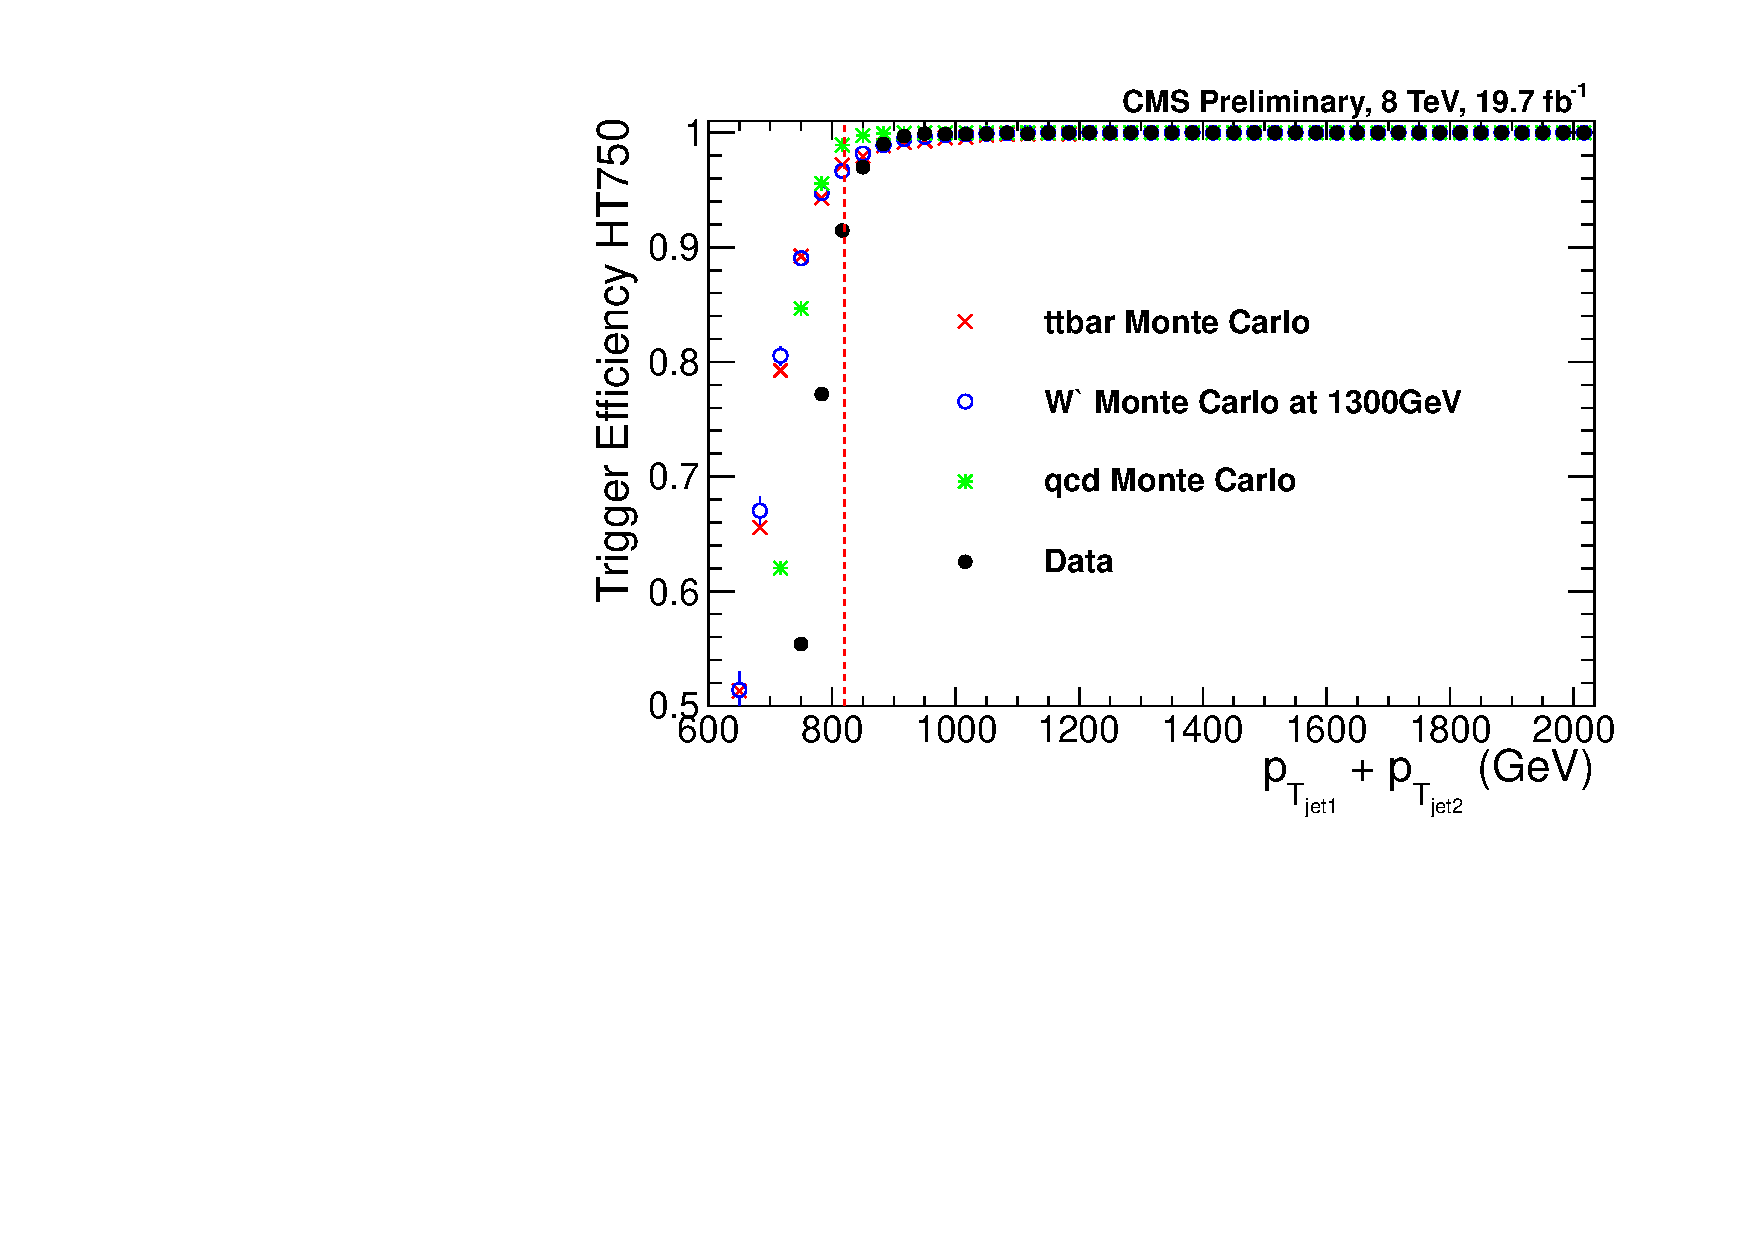
\includegraphics[width=0.9\textwidth]{AN-13-004/figs/Trigger_Comparison_Htdijet.pdf}
\caption{Trigger efficiency of \texttt{HLT\_HT750} measured as a function of the summed $\pt$ of the leading and sub-leading jets.  The red dashed line indicates the minimum for the analysis, 
at which point the trigger is nearly fully efficient.}
\label{figs:Trigger_Comparison_Ht}
\end{figure}

\section{Signal Characteristics}
\label{sec:sigchar}
\label{sec:GenBptCut}
The $\wpr$ boson of interest is very massive, and produces highly boosted top quarks.  The decay products of these top quarks become more collimated as the boost 
increases.  When the top decays hadronically, we observe one merged jet over the two distinct jets that would be detected at a lower boost.  This jet has a 
large characteristic radius and a distinct substructure.  This high energy jet merging is investigated in Figure \ref{figs:topmerge}.  Here, the `top candidate' 
is just the leading jet in the event.  It is also required to be hemispherically separated from a Monte Carlo truth b jet.  This jet is generally a merged W boson at low $\pt$ and a merged top at high $\pt$.
The `W candidate' (used for the bottom plots) is assembled from the pair of generator level non-b quarks that are close to the W mass (within 2.0~$\GeV$).  
The central feature of this analysis is using this jet merging to discriminate signal from background.

\begin{figure}[htcb]
\centering
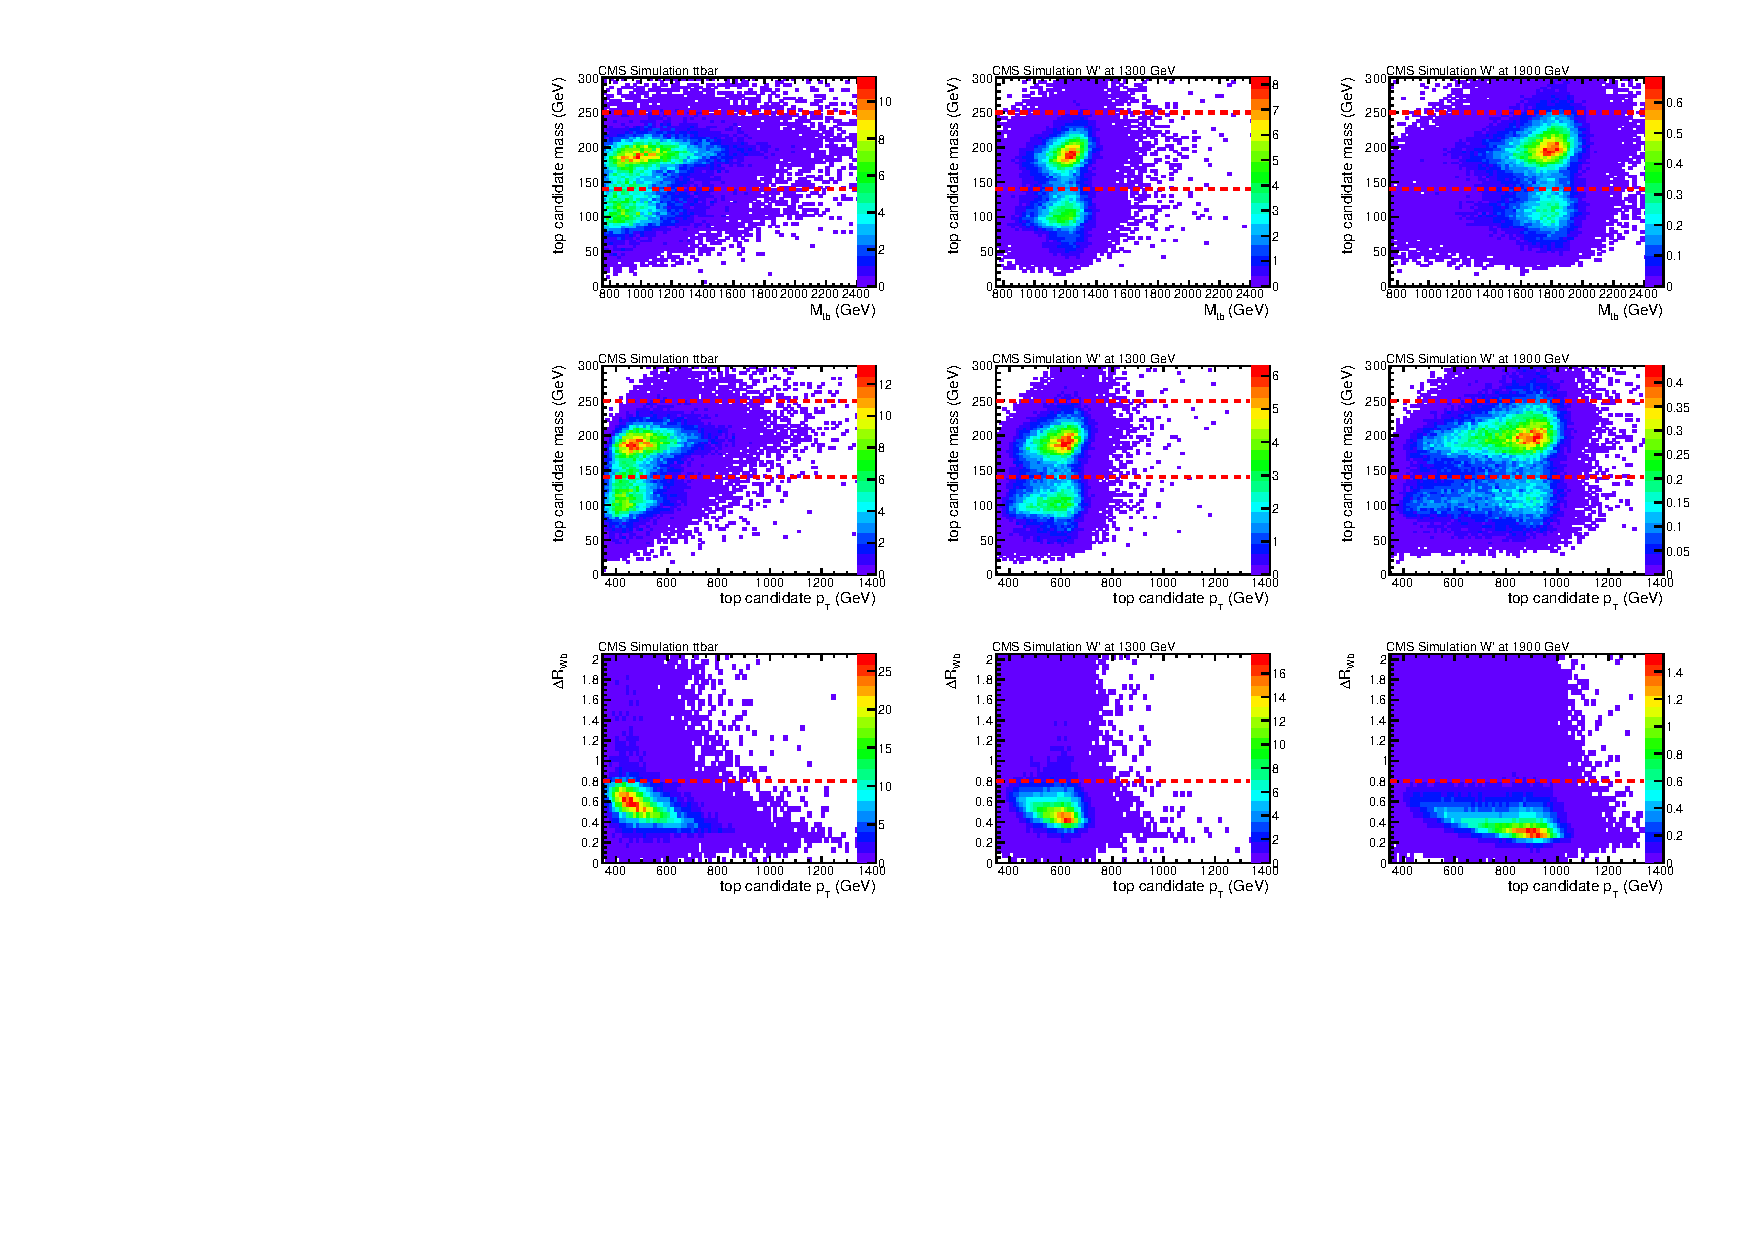
\includegraphics[width=0.9\textwidth]{AN-13-004/figs/topmerge.pdf}
\caption{Investigation of top merging within Monte Carlo samples of interest.  $\ttbar$ (left) $\wpr_R$ Monte Carlo at 1300$\GeV$ (middle) $\wpr_R$ Monte Carlo at 1900$\GeV$ (right).  The red lines on the top and middle plots indicate the top candidate mass cut in the full selection (see Section \ref{sec:toptagging}).  The red line on the bottom plots indicate the characteristic jet radius used to investigate fully merged top jets (see Section \ref{sec:reconstruction}).}
\label{figs:topmerge}
\end{figure}

We place a generator level $\pt$ cut on the b quark from the $\wpr$ decay in the left-handed and mixed-coupling $\wpr$ samples (see Section \ref{sec:signal}).  
To investigate the effect of this pre-selection, we look at the effect of an even tighter cut.  
Figure \ref{figs:genptcut} shows the ratio of generator level b $\pt$ cuts.  
The denominator requires a generation level pt cut of 200 $\GeV$ and the numerator requires a generation level pt cut of 230 $\GeV$.  
This ratio is parameterized in the $\pt$ of the CA8 jet that the generation particle is matched to ($\mathrm{\Delta R  < 0.5}$ is used for matching).
The turn on of this tighter cut is well below the analysis level cut of 370$~\GeV$.  Thus, the effect of the generation level b $\pt$ cut 
on selections requiring the analysis level $\pt$ cut is negligible.  

\begin{figure}[Htcb]
\centering
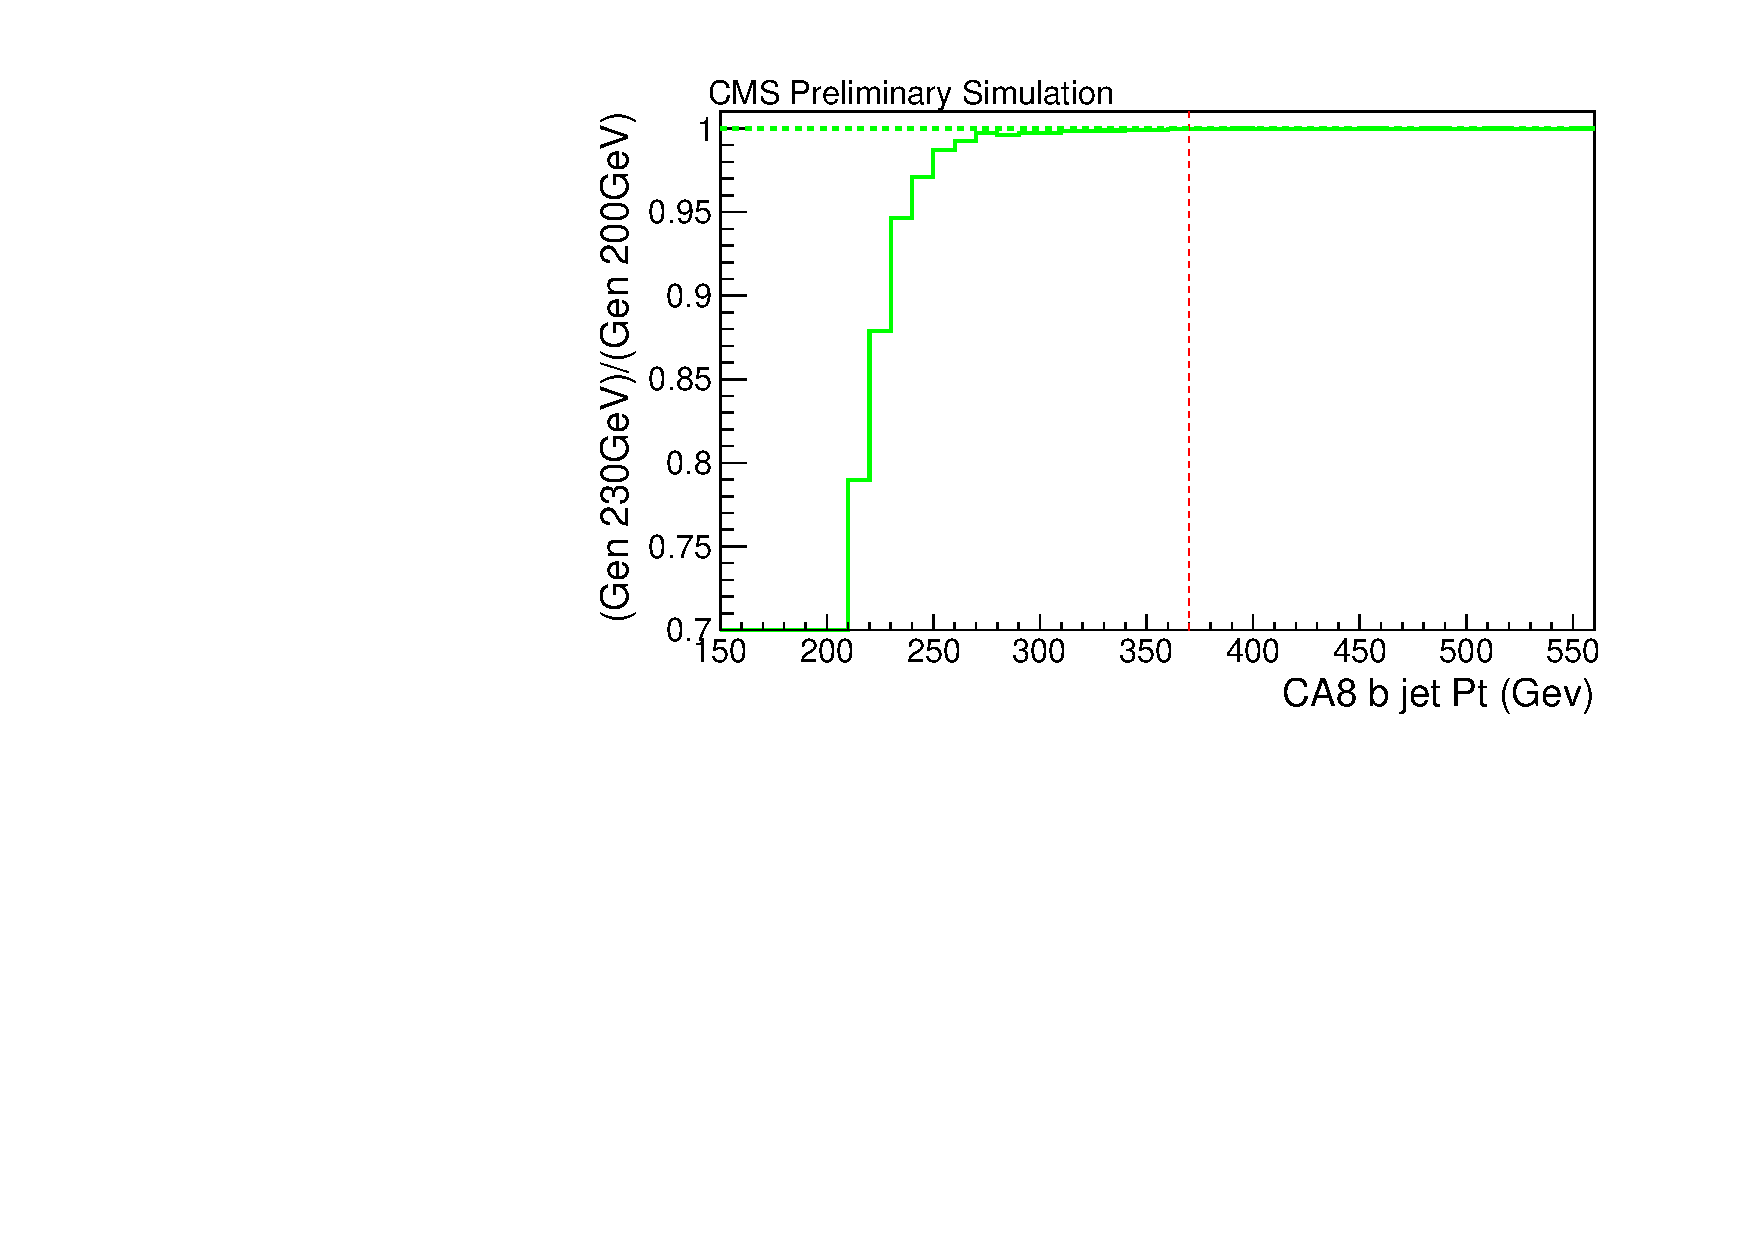
\includegraphics[width=1.0\textwidth]{AN-13-004/figs/bjetptcut.pdf}
\caption{Ratio of CA8 $\pt$ using the generation level b pt cut of 230$~\GeV$ and 200$~\GeV$.  The red line is the analysis level $\pt$ cut of 370$~\GeV$.  The sample used for this study is $W`_{LR}$ at 1300$~\GeV$}
\label{figs:genptcut}
\end{figure}



\section{Jet Reconstruction}
\label{sec:reconstruction}
All data is reconstructed using CMSSW 5.3.x, and uses jet energy corrections from \verb!FT_53_V21_AN5! \cite{CMS-DP-2013-033}.  The Particle Flow reconstruction algorithm is used 
to reconstruct all data and Monte Carlo samples used for the analysis.  This algorithm uses information from all sub-detectors 
to categorize particles as muons, electrons, photons as well as charged and 
neutral hadrons.  Charged hadrons identified as pileup are removed from the inputs to the jet clustering algorithms by Charged Hadron Subtraction (CHS).
Pileup vertices are identified as vertices that have a lower $\pt$ than the primary vertex.  Isolated charged leptons are removed,
and neutral pileup components are removed with a residual area-based method.  For more detail, see \cite{7tevZprime}.  
The PF candidates are then used to create 'Particle Flow jets' as follows.  Jet clustering is performed 
with a sequential recombination algorithm which compiles jets by merging the minimum of 
$\mathrm{d_{ij} = min(k_{Ti}^{2m},k_{Tj}^{2m})\Delta _{ij}/R}$ where $\mathrm{\Delta _{ij} = \sqrt{(y_i-y_j)^2 + (\phi _i-\phi _j)^2}}$.
  We use the Cambridge-Aachen (CA) \cite{CAcambridge,CAaachen} algorithm implemented by FastJet 3 \cite{fastjet1,fastjet2}, 
which assigns a value of $\mathrm{m = 0}$, and thus is not weighted by $\pt$.  An R value 
of 0.8 is used for the analysis.  The CA algorithm has been shown to be more efficient than the 
the $\mathrm{k_{T}}$ and the anti-$\mathrm{k_{T}}$ algorithms for finding hard subjets \cite{catop_cms}.

%The corrections for the CA $R=0.8$ jets are derived from the
%anti-$k_{\mathrm T}$ $R=0.7$ jet algorithm. 
We use anti-$\mathrm{k_{T}}$ jet energy corrections for all jets in the analysis. 
The jet energy corrections derived are adequate for the CA $\mathrm{R=0.8}$ jet algorithm for the jet momenta
considered here as can be seen from 7~$\TeV$ studies in simulation comparing AK5 and CA8 jets \cite{7tevZprime}.  
We use the 2012 prescription for jet energy corrections\cite{JEC2012}.  We apply AK7 
Particle Flow with charged hadron subtraction 
(AK7PFchs) jet energy corrections for all data and Monte Carlo samples.

\section{Event Pre-selection}
\label{sec:pre-selection}
The following pre-selection is applied:

\begin{itemize}
\item The event must have a good primary vertex as computed by a deterministic annealing filter (DAF)
($\vert z_\text{Primary Vertex}\vert < 24$ cm, $N_\text{DOF} > 6$).
\item Two jets with $|y| < 2.4$
\item Only two jets with $\pt > 150~\GeV$
\item Leading Jet $\pt > 450~\GeV$ \& Sub-leading Jet $\pt > 370~\GeV$
\item Loose Particle Flow jet identification \cite{jetid} is applied
\item Leading and sub-leading jet are separated by $|\Delta y| < 1.6$
	\begin{itemize}
	\item This cut is described in Section \ref{sec:deltarapidity}
	\end{itemize}
\item Beam background events are removed using the following requirements:
        \begin{itemize}
        \item In events with at least 10 tracks, a minimum of 25\% of
          these tracks must be high purity tracks.
        \end{itemize}
\end{itemize}


The requirement that there are only two jets with $\pt > 150~\GeV$ is useful for vetoing "three-prong" trijet events, which could impact the kinematics of the top-W candidate invariant mass 
distribution and bias the background estimate. 

\section{$\ttbar$ $\pt$ Re-weighting}
\label{sec:ttptrw}
In order to correct for known differences in the top $\pt$ spectrum between data and $\ttbar$ Monte Carlo, we re-weight Monte Carlo using the Generator level $\pt$ of the top and anti-top with the recommended prescription.  
With $\mathrm{p_{T_{t}}}$ and $\mathrm{p_{T_{\overline{t}}}}$ being the generator $\pt$ of the top and anti-top respectively, the scale factor applied to each event in the $\ttbar$ Monte Carlo expectation is:
\begin{eqnarray}
SF =\sqrt{e^{0.156-.00137p_{T_{t}}} \times e^{0.156-.00137p_{T_{\overline{t}}}}}
\end{eqnarray}
Although this procedure was not designed for the kinematic range in our analysis, we prefer to use the prescription as it is more consistent with our measurement of the $\ttbar$ normalization (see Section \ref{sec:ttbarsideband}).


\section{Pileup Correction}
\label{sec:pileup}
We re-weight our Monte Carlo samples to account for differences due to pileup using the recommended procedure.  
To create a scale factor for number of primary vertices, we use Monte Carlo truth to extract the number of pileup interactions.  
Then we compare this to the mean number of interactions per crossing from data.  
This is extracted using the pileup distribution from the rereco datasets listed in table \ref{table:datasets}.  
For this calculation we use the suggested minbias cross-section of 69.4 mb.  The scale factor is then 
the data distribution divided by the distribution in Monte Carlo and is applied to the signal and $\ttbar$ Monte Carlo samples to improve 
data to Monte Carlo agreement.
Figure \ref{figs:npvweight} shows the distribution of reconstructed primary vertices in Data, $\ttbar$,
and signal Monte Carlo before and after the re-weighting has been applied. The pileup correction has very little effect on the eventual $\mathrm{M_{tb}}$ full selection, as 
seen in Figure \ref{figs:pileup3}, for $\wpr_R$ signal Monte Carlo at the 1900$~\GeV$ mass point. Similarly, there is little effect 
$\ttbar$ Monte Carlo as can be seen in Figure \ref{figs:pileup3ttbar}.  
A study has been conducted to investigate the effect of the suggested systematic uncertainty of 5\% on the  as can be seen in Chapter \ref{sec:systematics}.  
Figure \ref{figs:PUplots} shows the number of primary vertices in data and signal Monte Carlo with respect to discrimination variables used to separate signal from background.

\begin{figure}[Htcb]
\begin{center}
\subfigure{\label{figs:sub_data}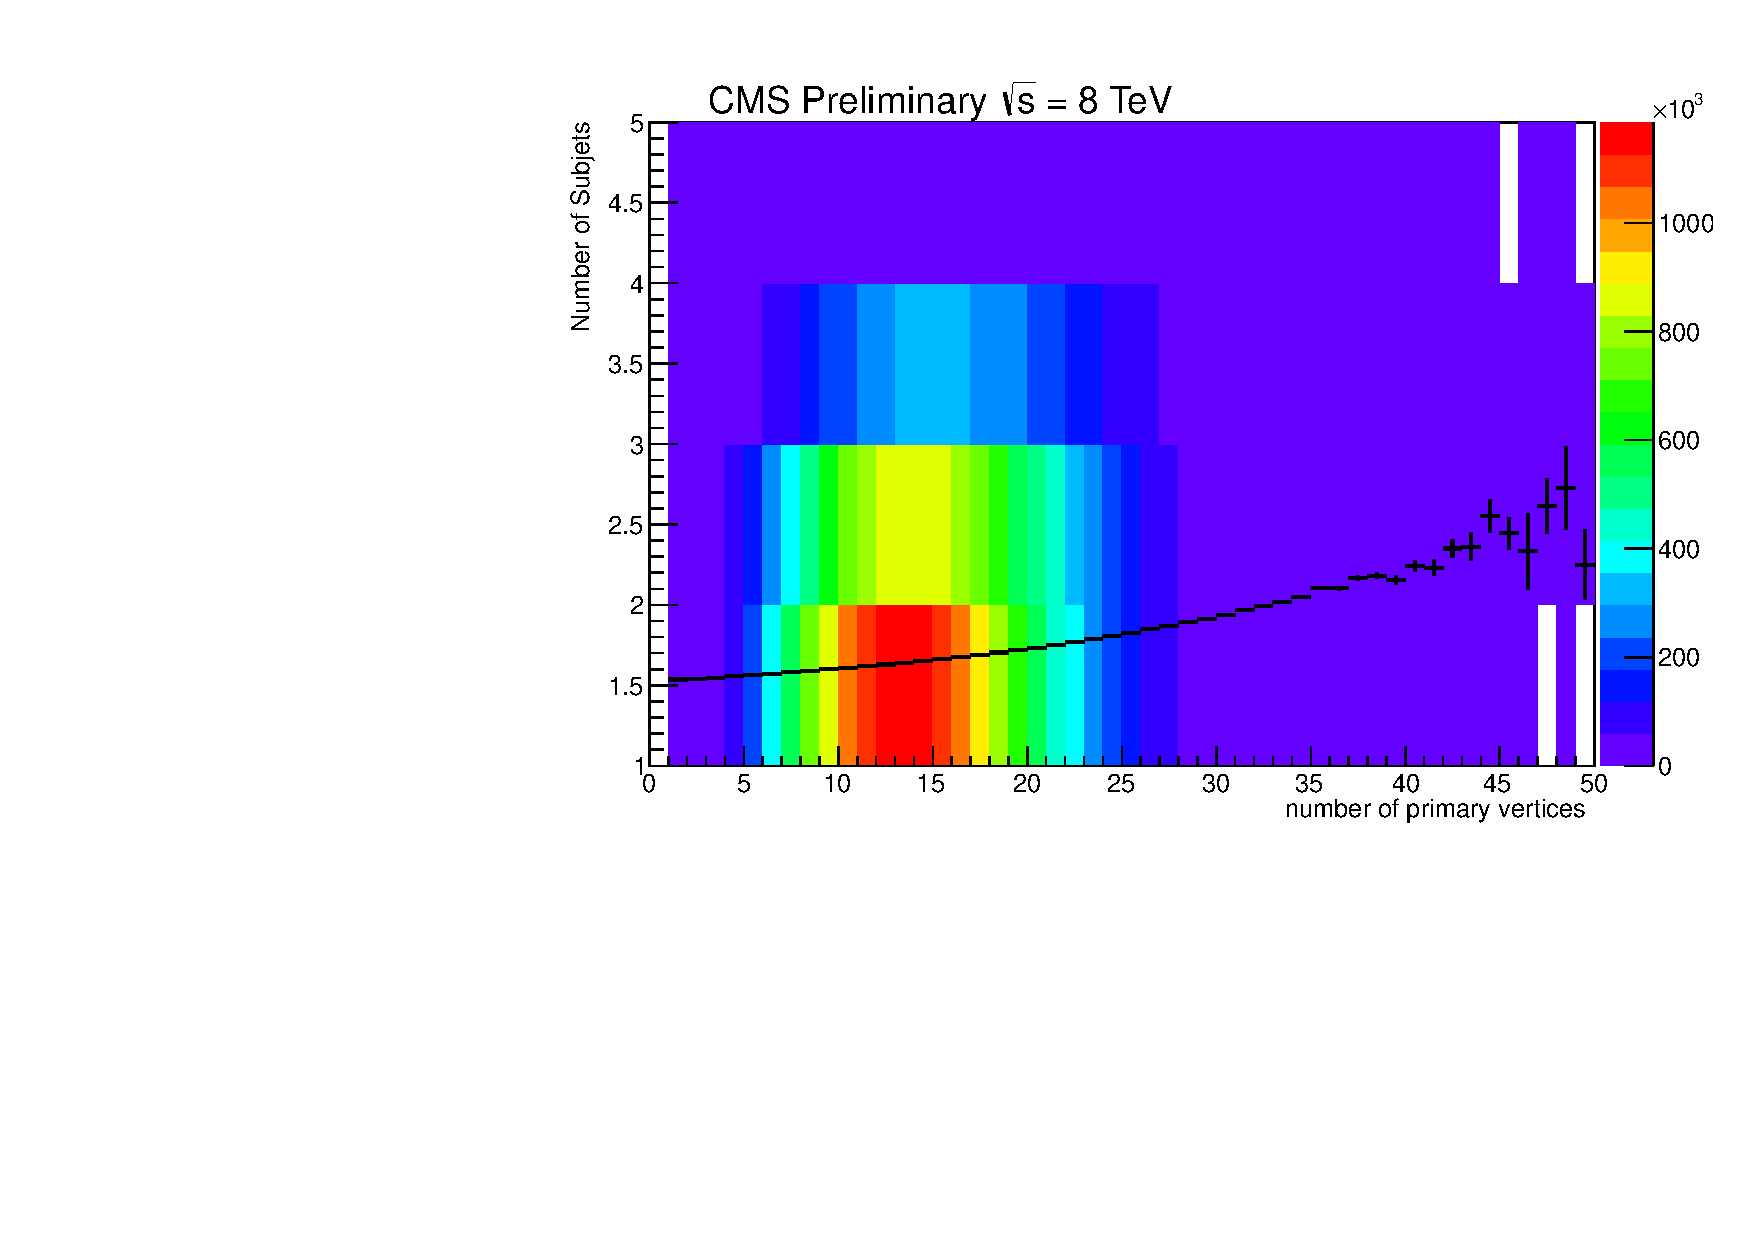
\includegraphics[width=0.4\textwidth]{AN-13-004/figs/sub_data.pdf}}
\subfigure{\label{figs:sub_signal}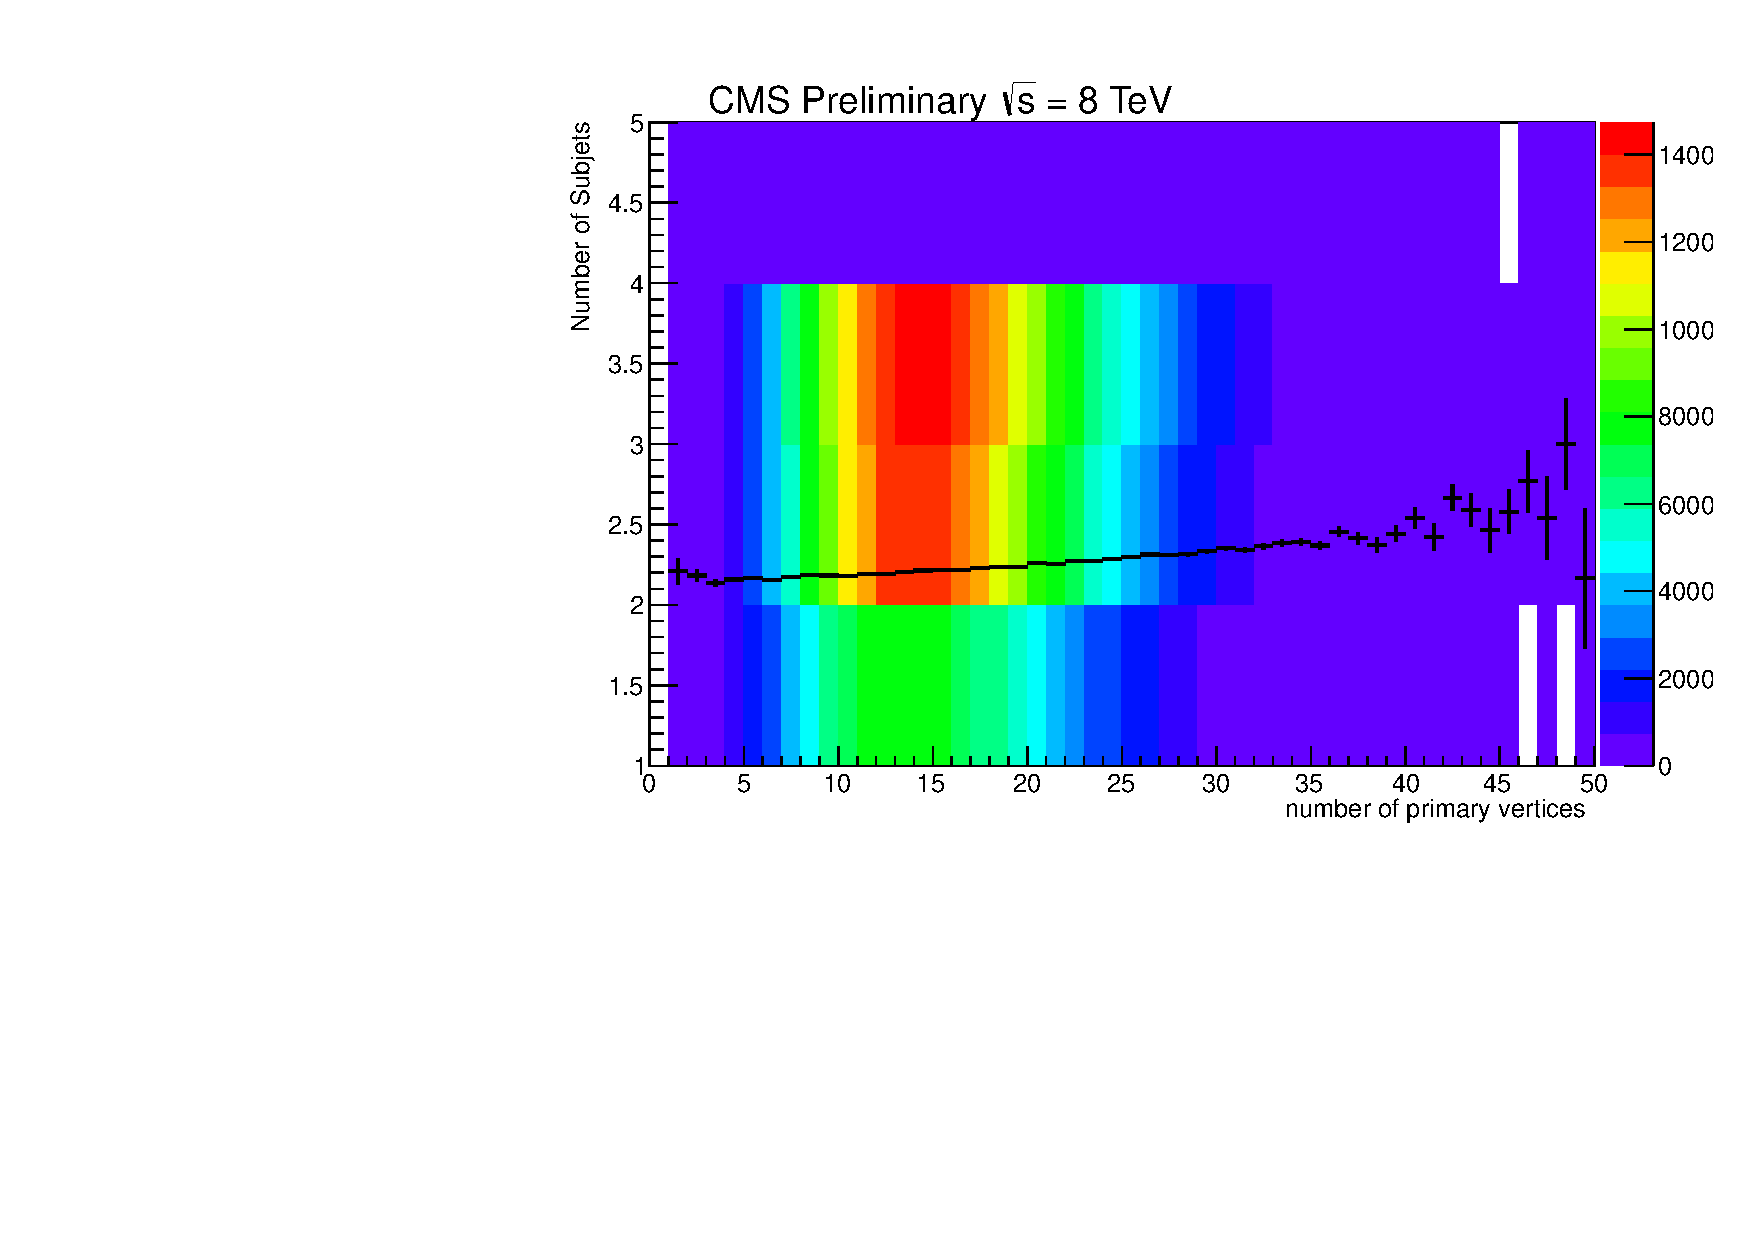
\includegraphics[width=0.4\textwidth]{AN-13-004/figs/sub_signal.pdf}}\\
\subfigure{\label{figs:min_data}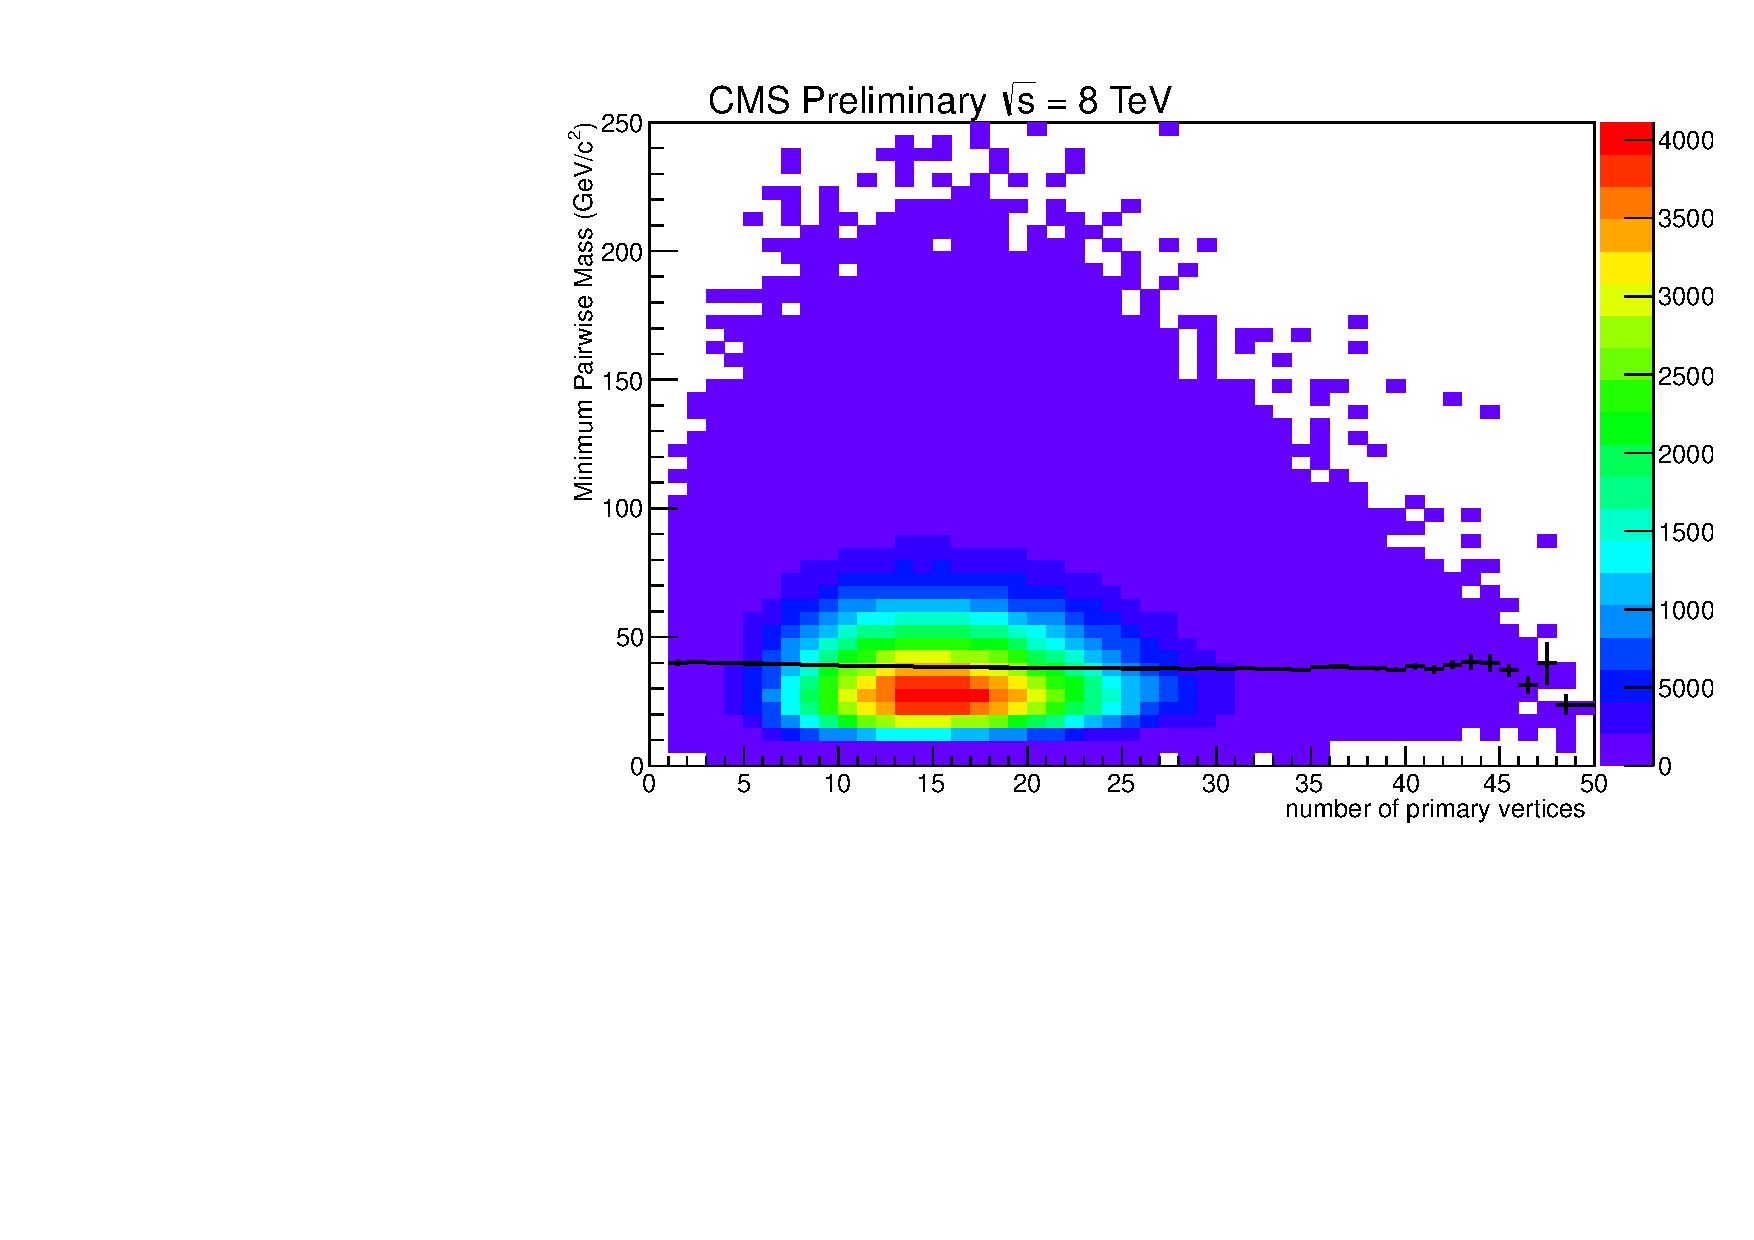
\includegraphics[width=0.4\textwidth]{AN-13-004/figs/min_data.pdf}}
\subfigure{\label{figs:min_signal}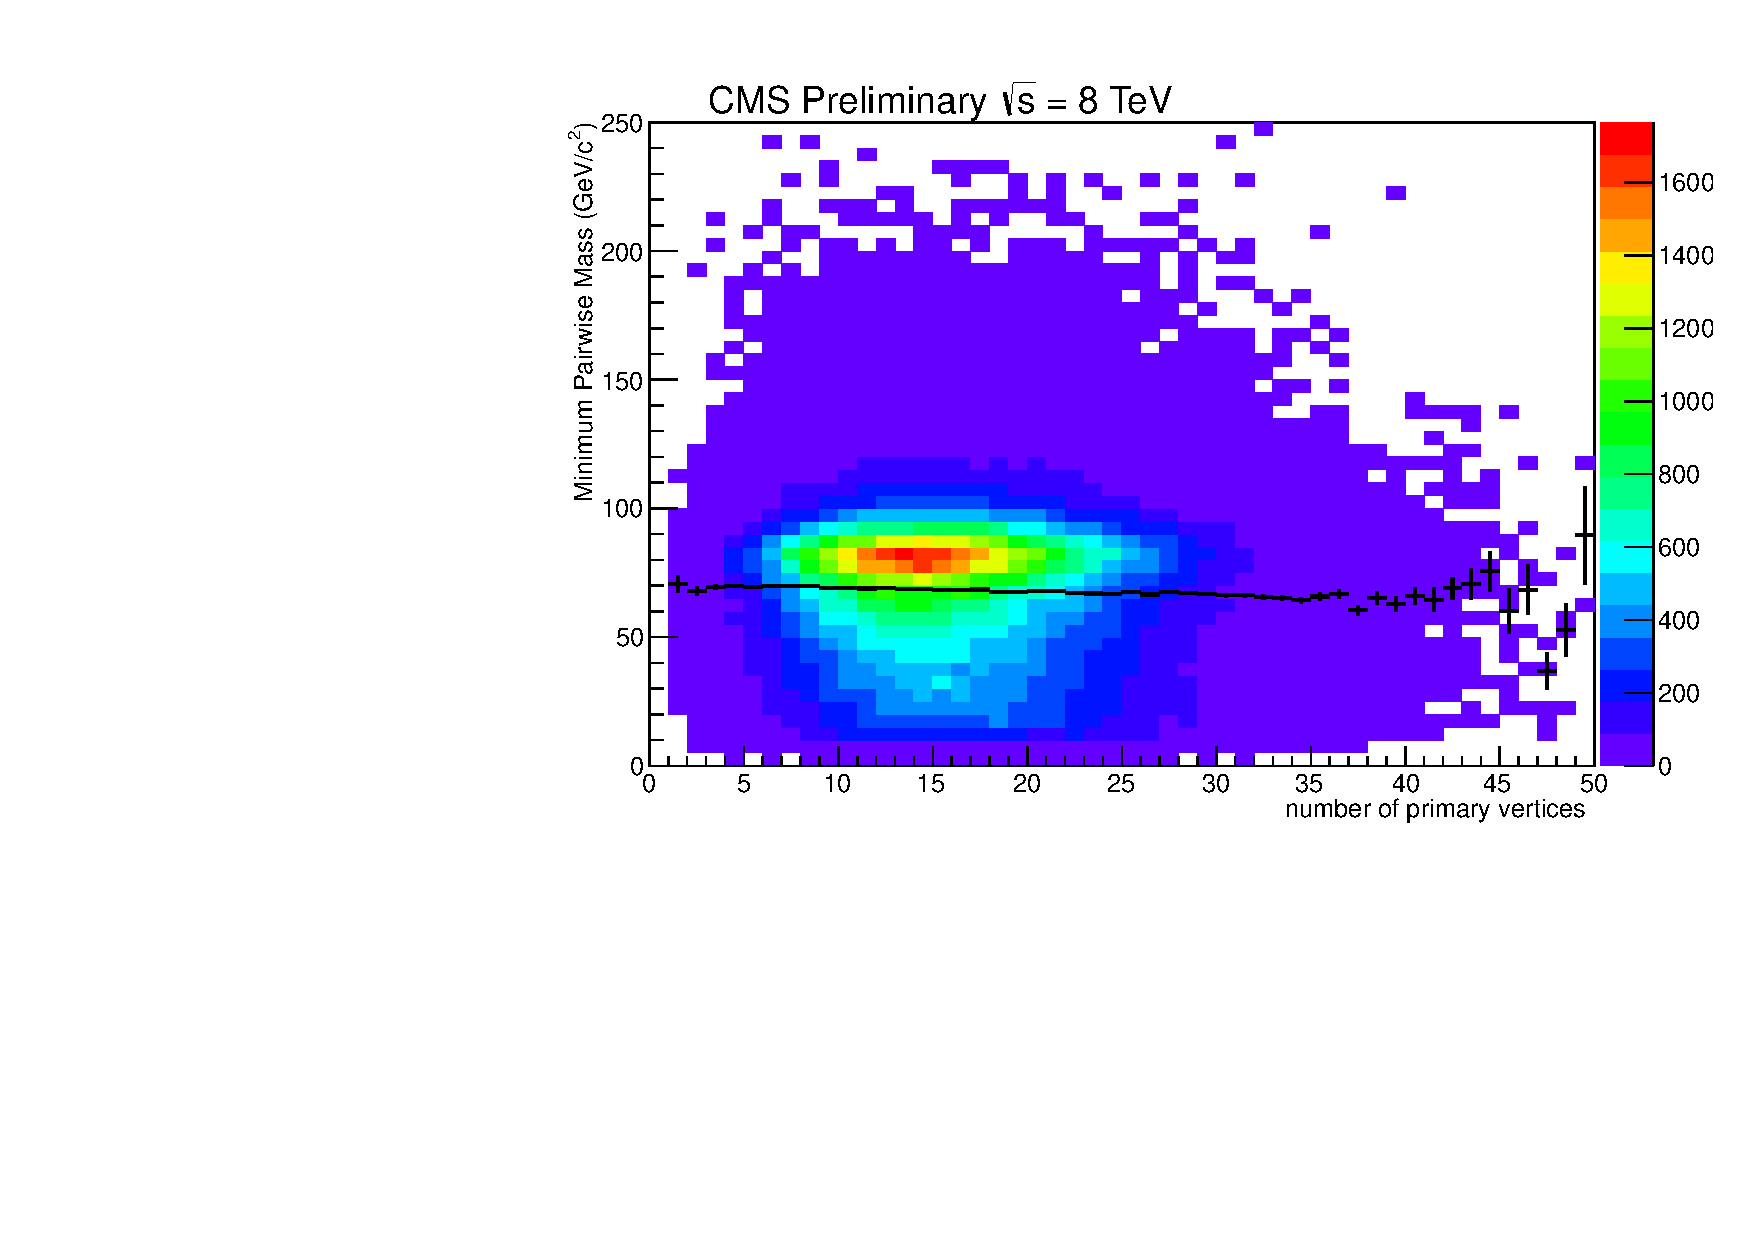
\includegraphics[width=0.4\textwidth]{AN-13-004/figs/min_signal.pdf}}\\
\subfigure{\label{figs:top_data}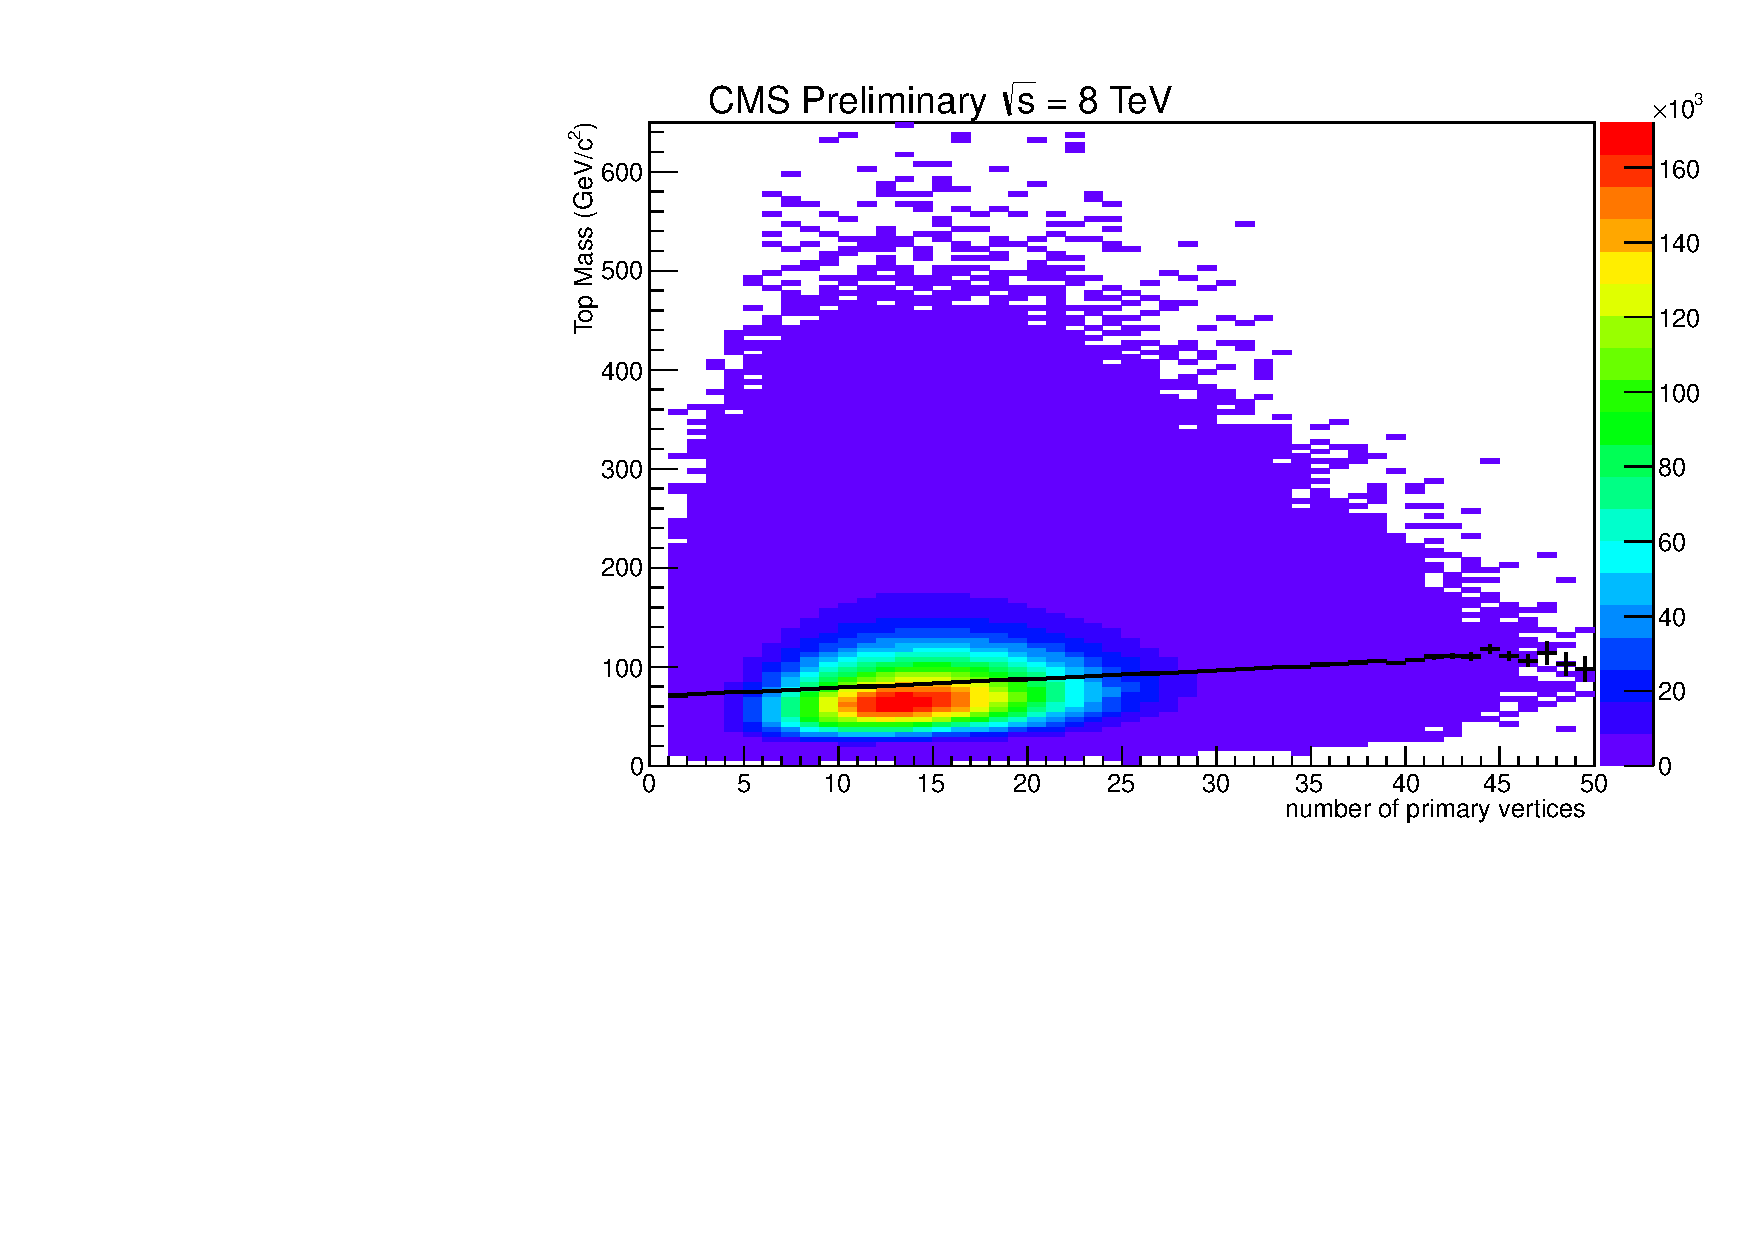
\includegraphics[width=0.4\textwidth]{AN-13-004/figs/top_data.pdf}}
\subfigure{\label{figs:top_signal}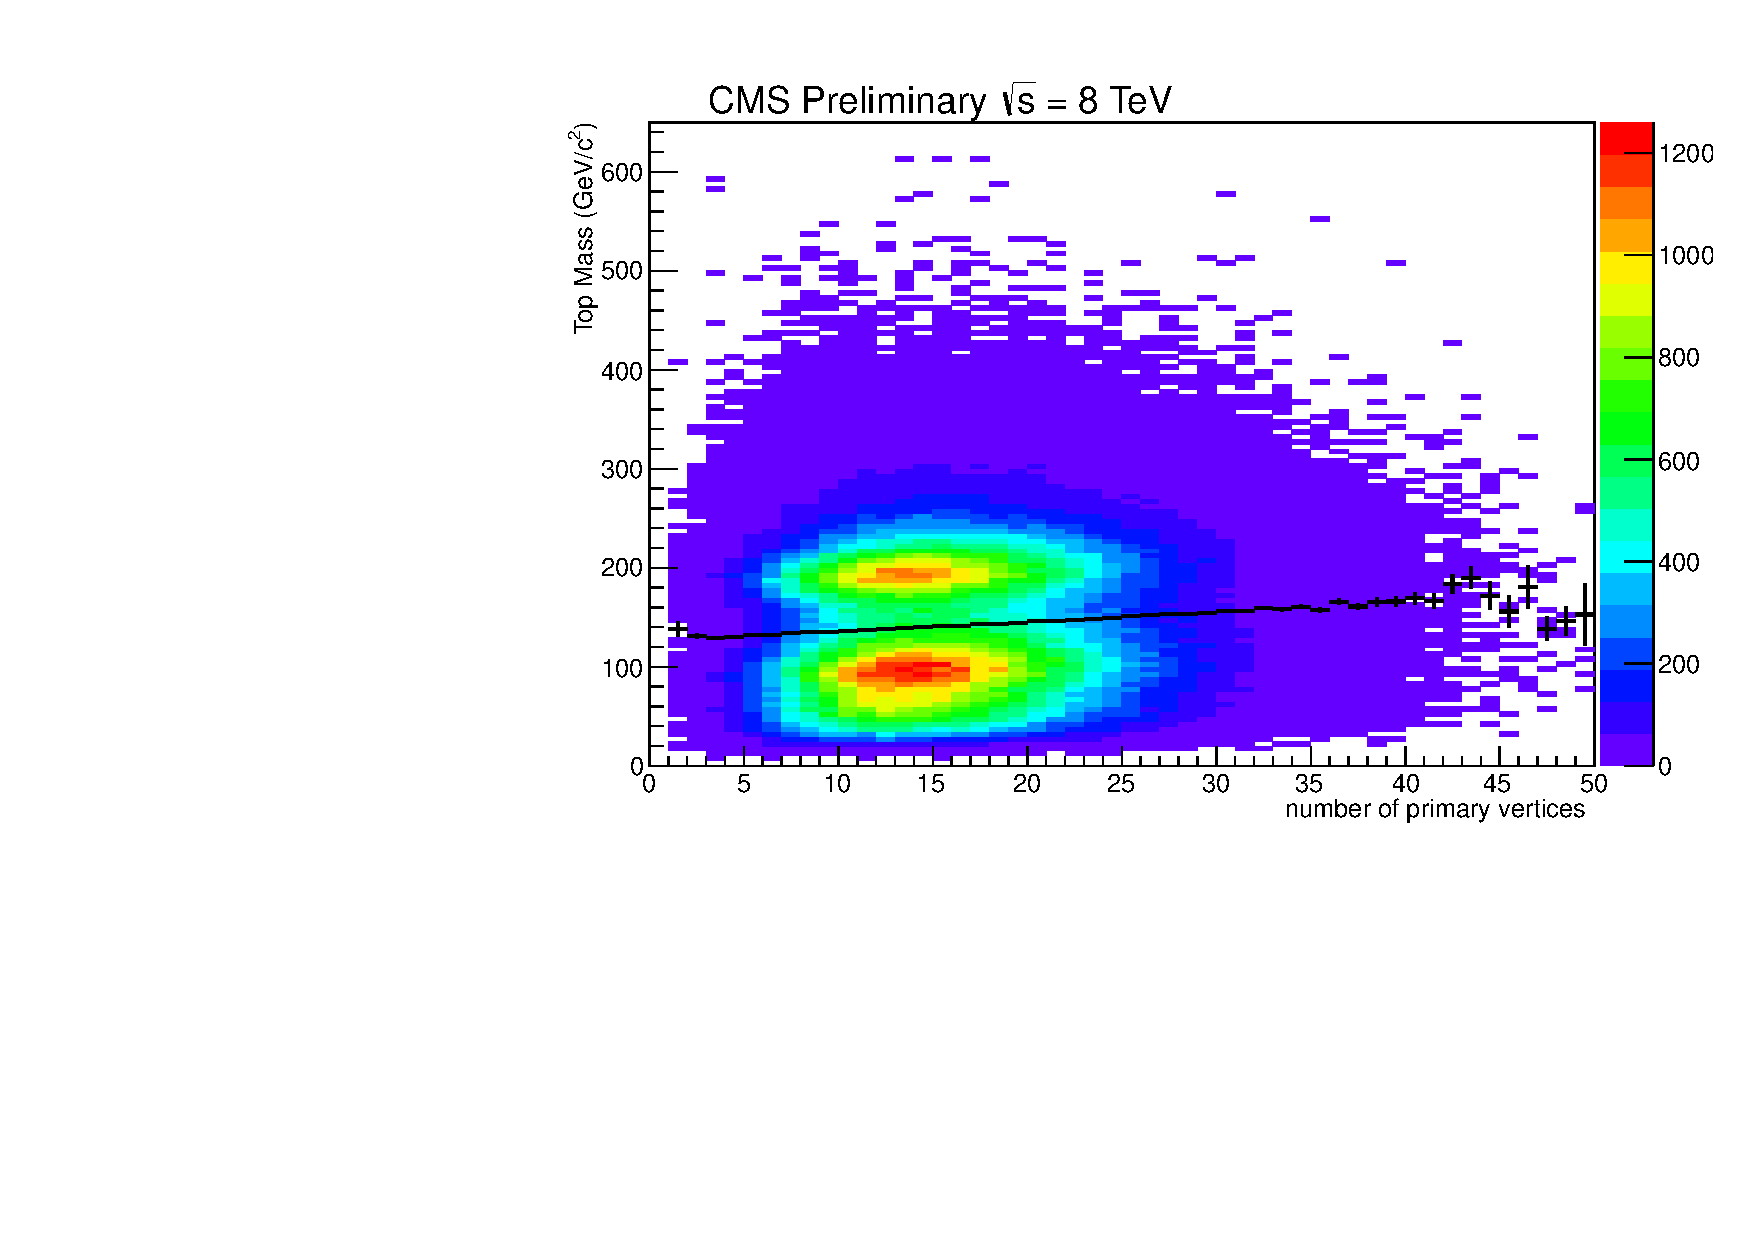
\includegraphics[width=0.4\textwidth]{AN-13-004/figs/top_signal.pdf}}\\
\subfigure{\label{figs:tag_data}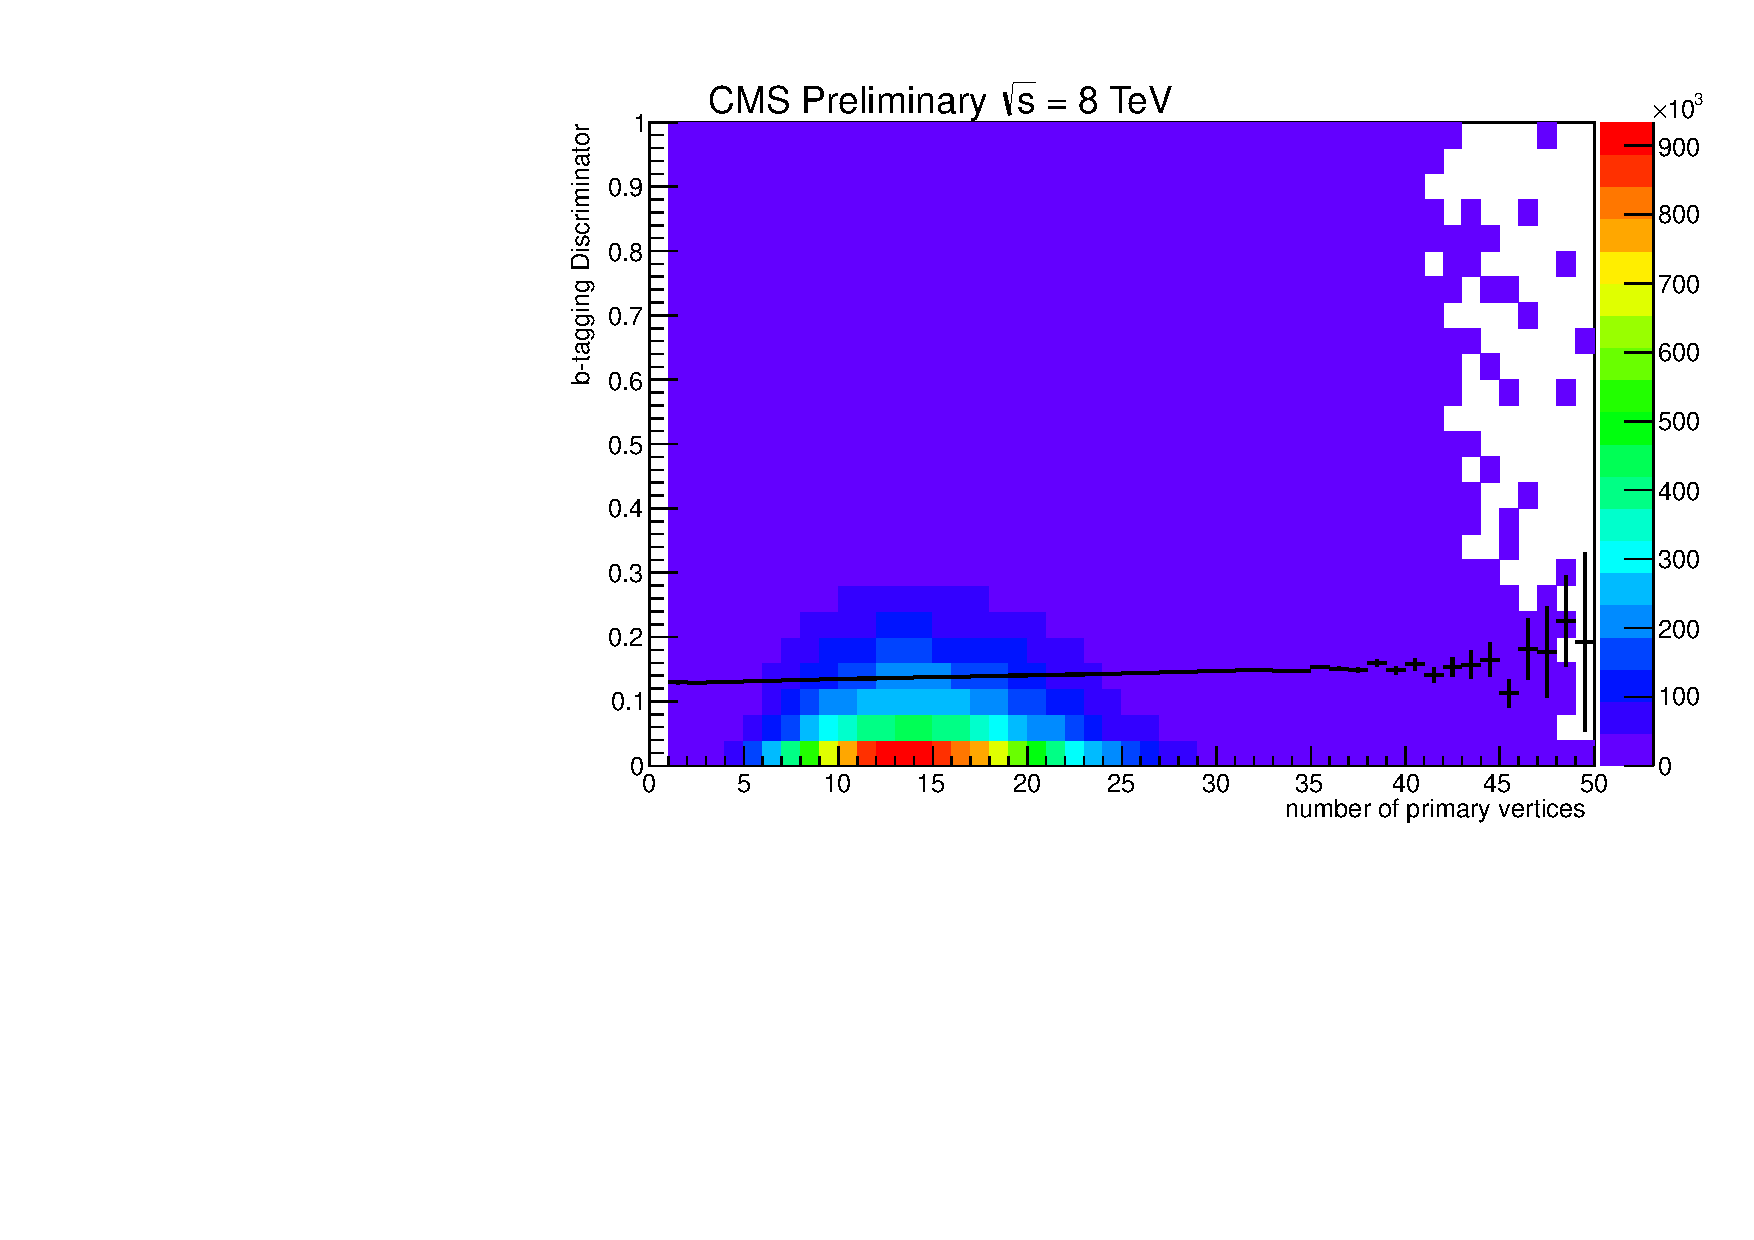
\includegraphics[width=0.4\textwidth]{AN-13-004/figs/tag_data.pdf}}
\subfigure{\label{figs:tag_signal}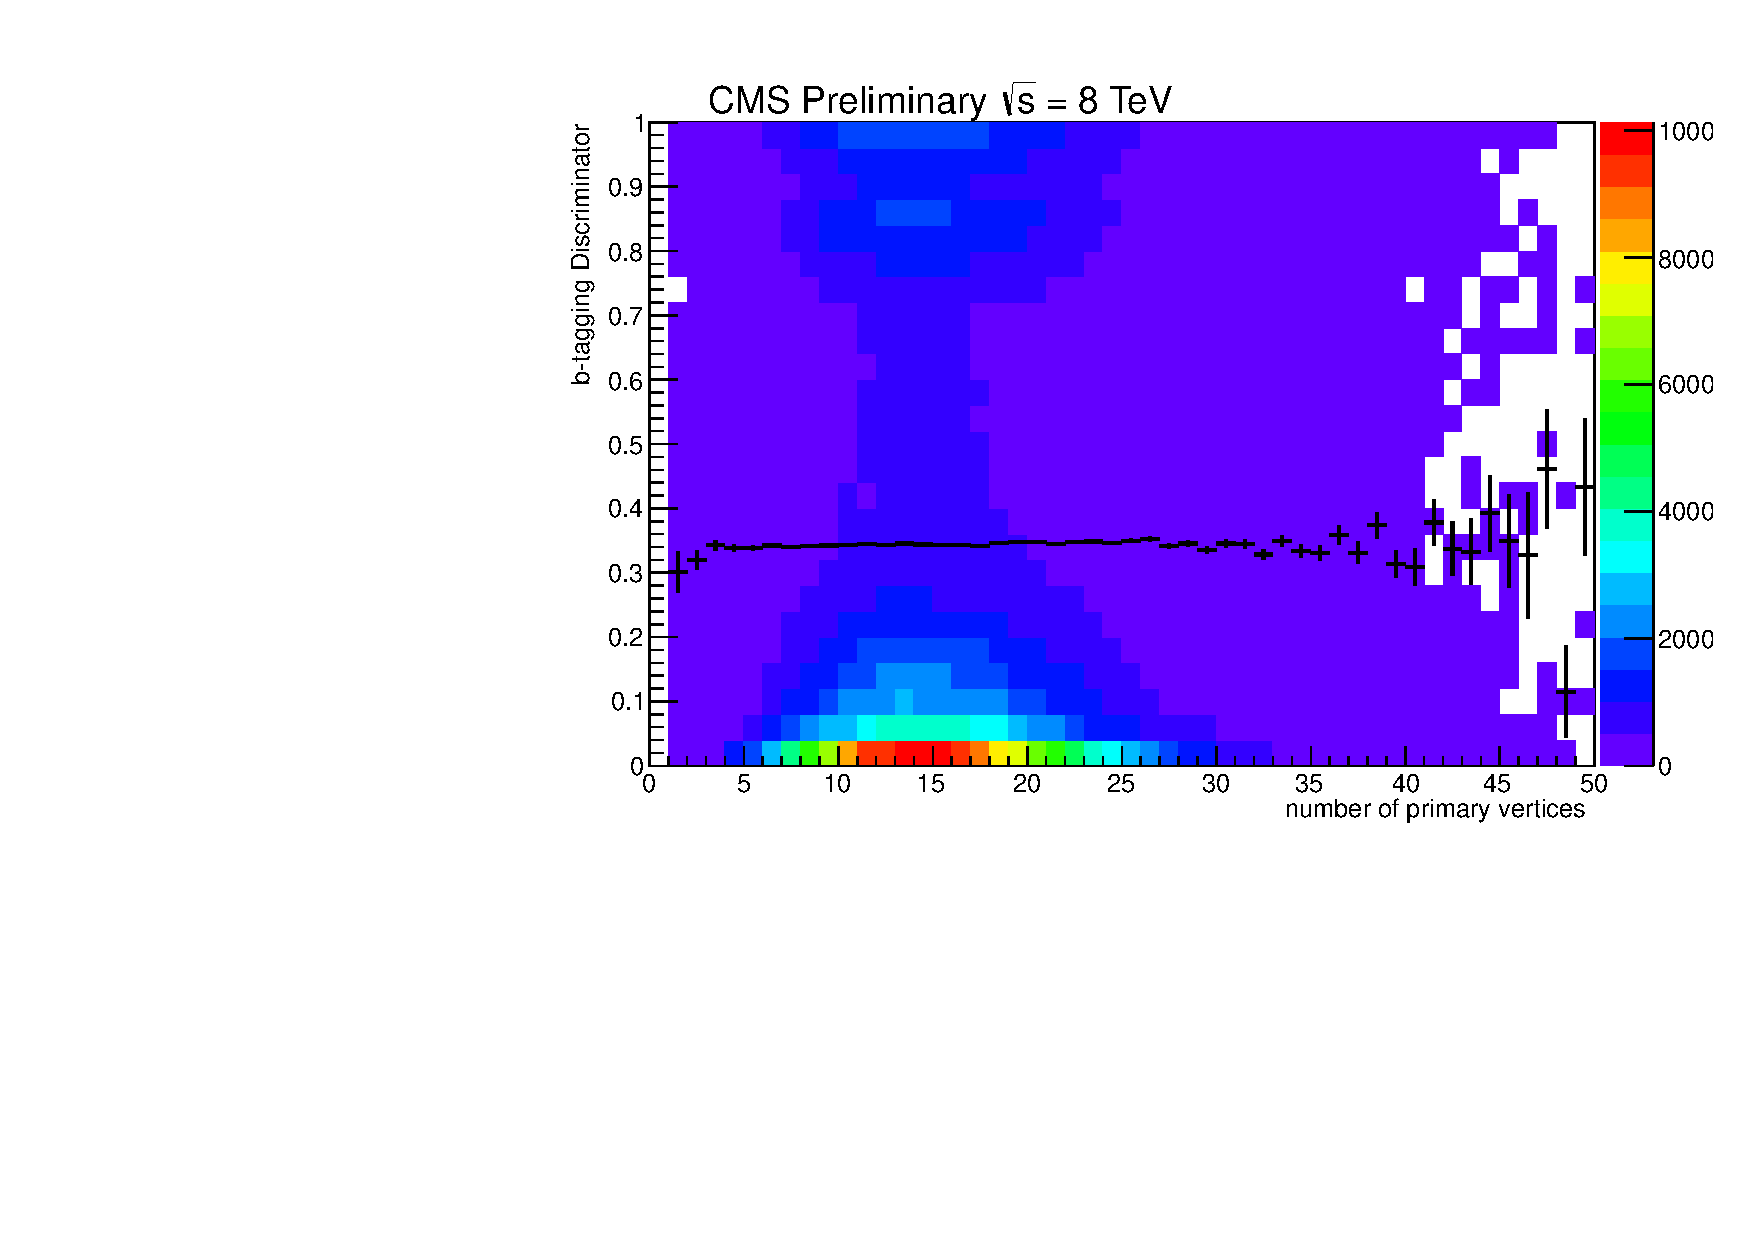
\includegraphics[width=0.4\textwidth]{AN-13-004/figs/tag_signal.pdf}}
\caption{
Number of primary vertices in data and signal Monte Carlo vs
(a) Number of Subjets  
(b) Minimum Pairwise Mass
(c) Top Mass
(c) CSV b discriminant 
}
\label{figs:PUplots}
\end{center}
\end{figure}


\begin{figure}
\begin{center}
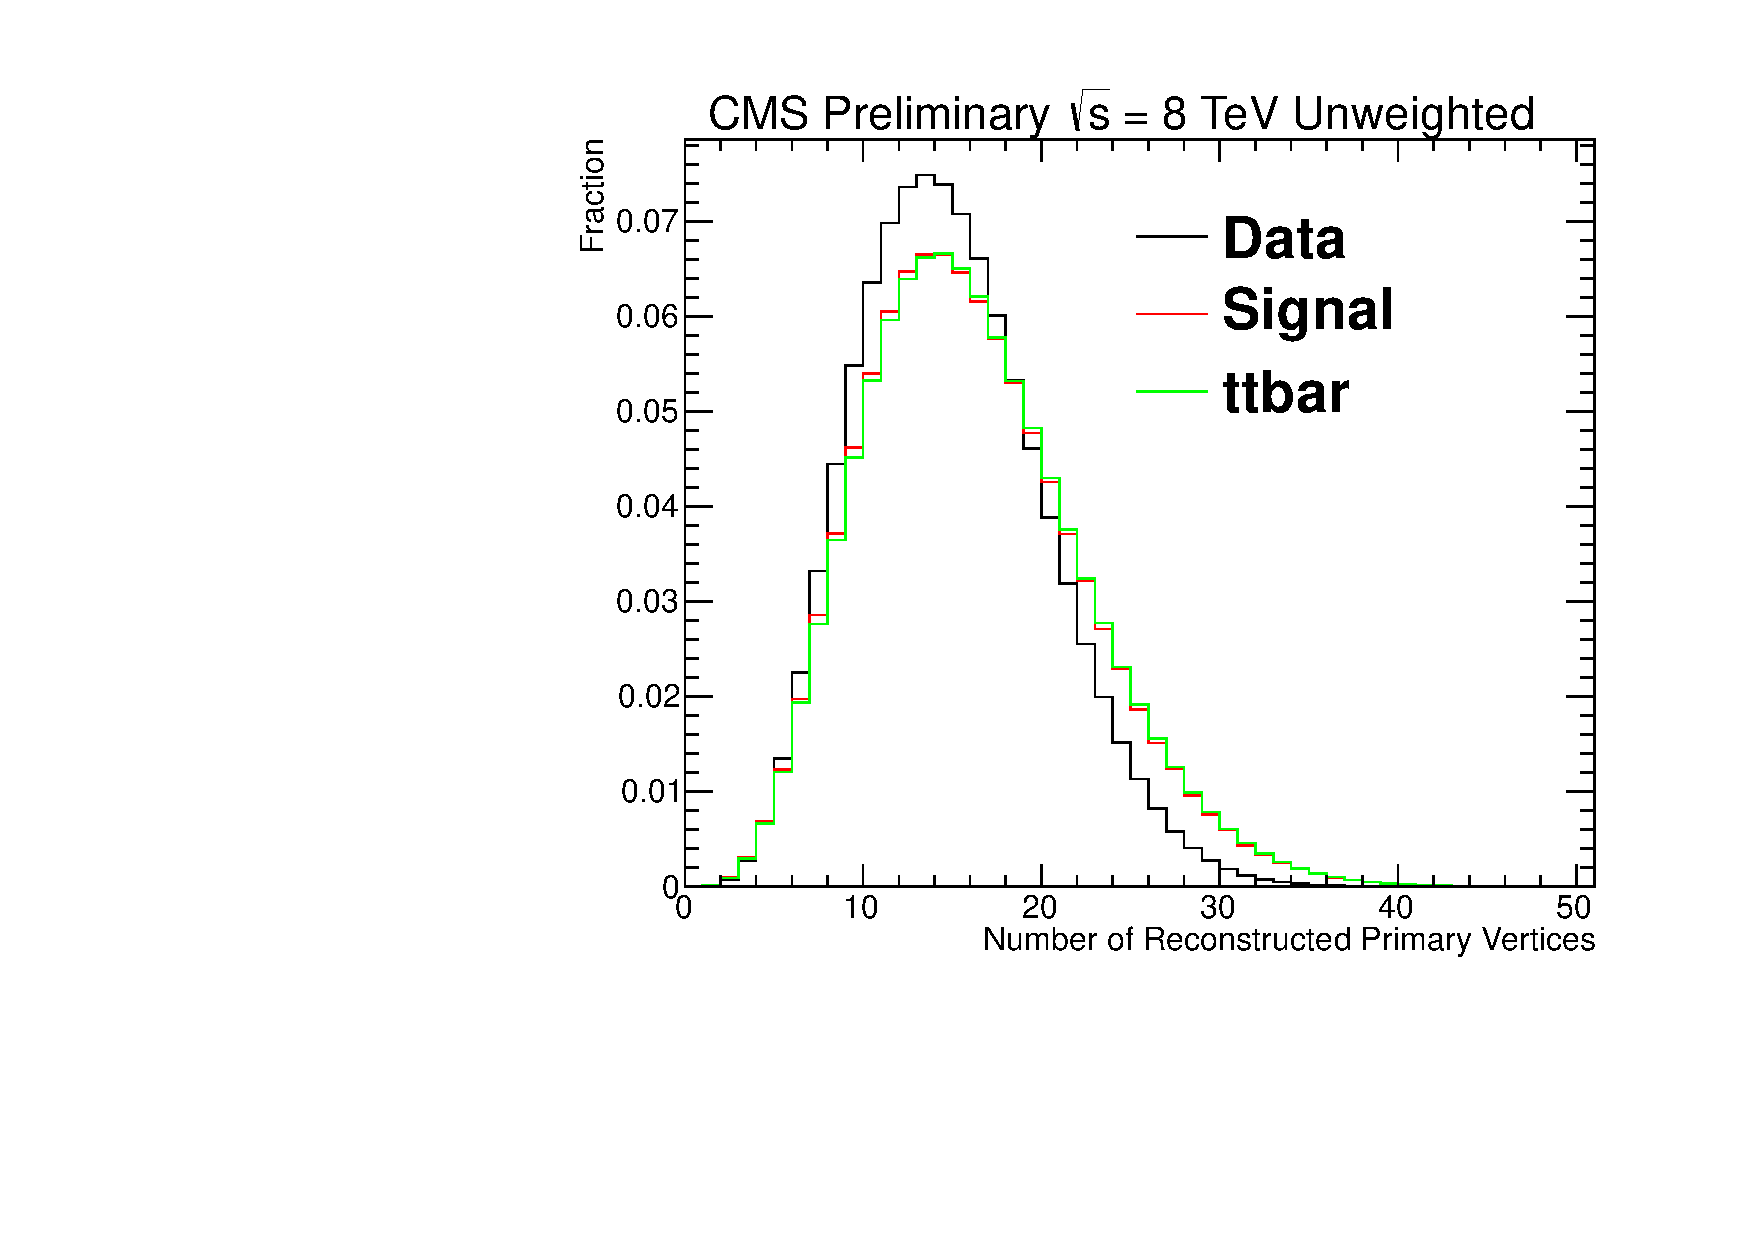
\includegraphics[width=0.7\linewidth]{AN-13-004/figs/npvuw.pdf}\\
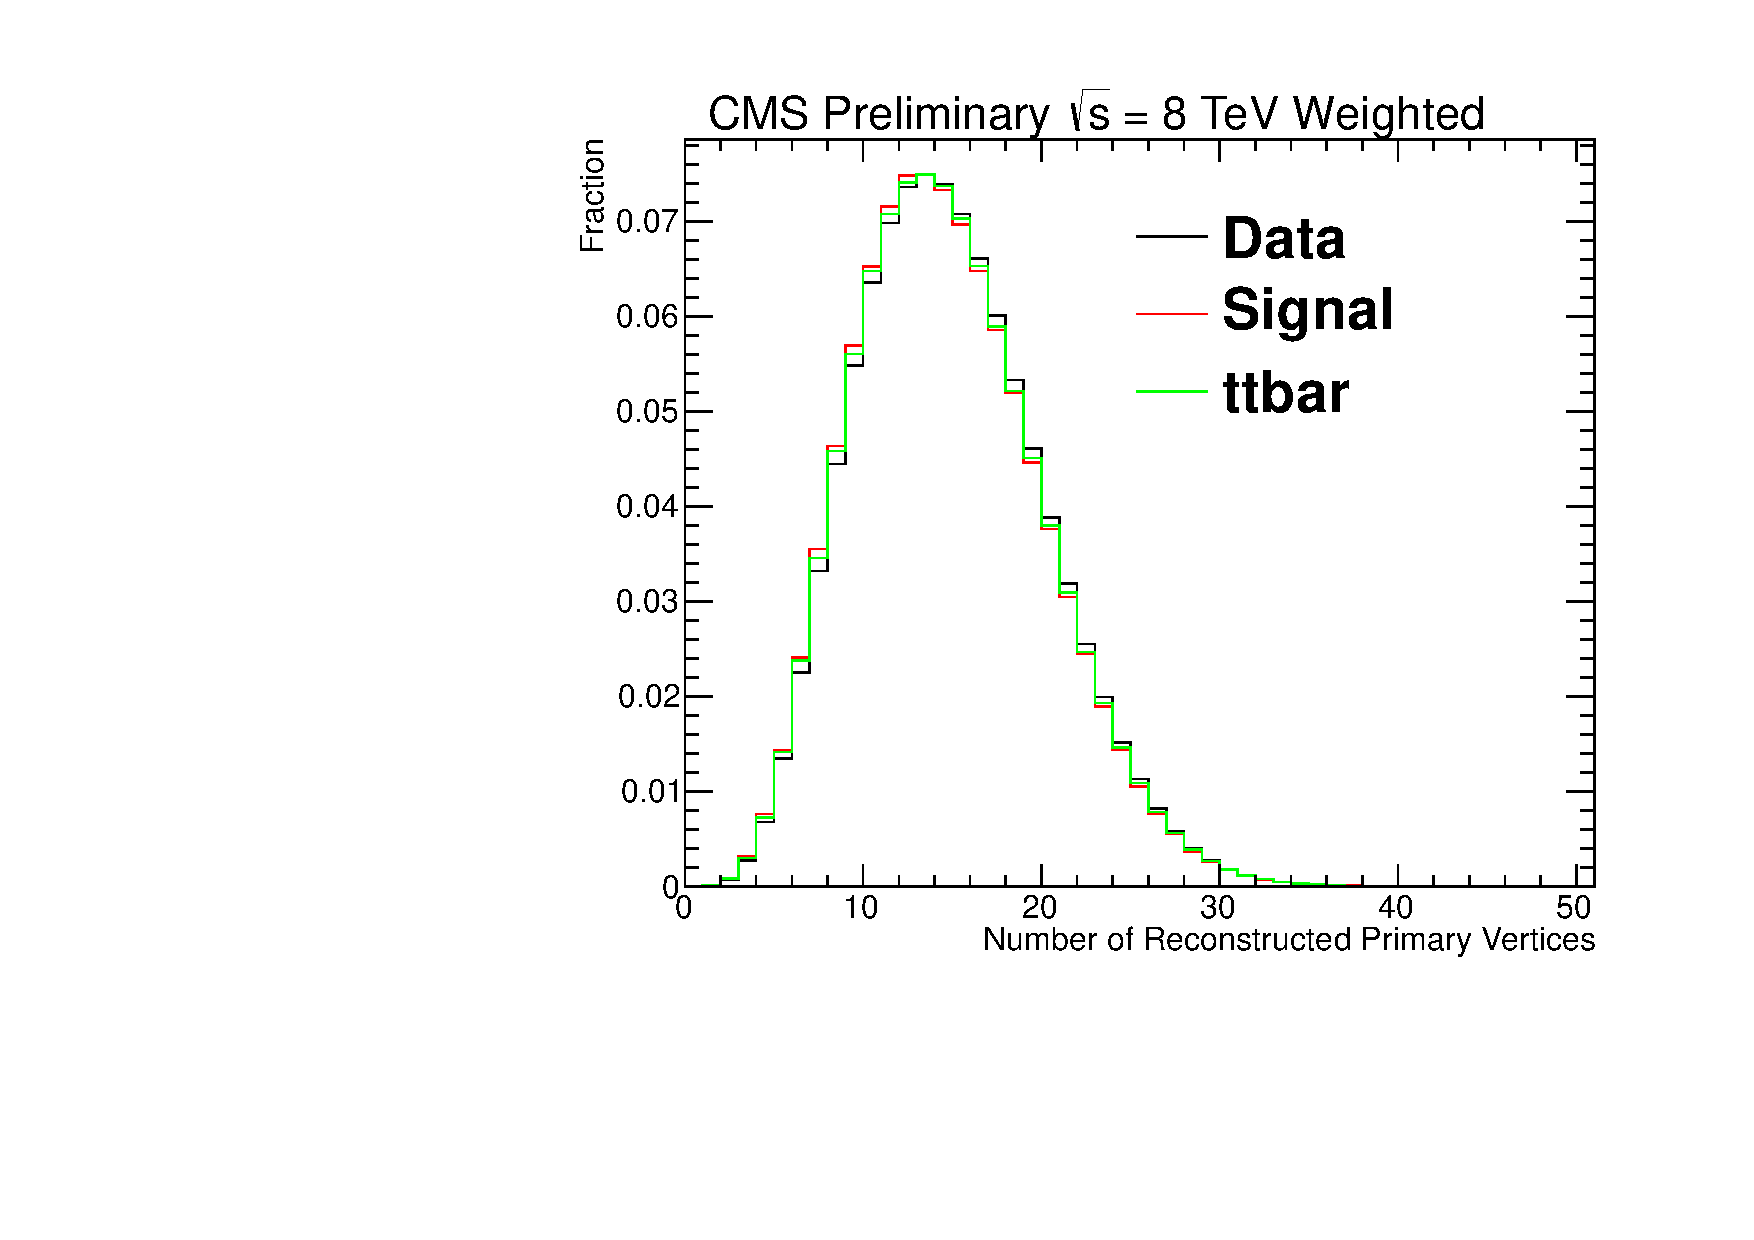
\includegraphics[width=0.7\linewidth]{AN-13-004/figs/npvw.pdf}
\end{center}
\caption{Number of reconstructed primary vertices before pileup re-weighting (top) and after pileup re-weighting (bottom).  Here, no analysis cuts have been applied and the signal mass point is 1900$~\GeV$}
\label{figs:npvweight}
\end{figure}

\begin{figure}[htcb]
\centering
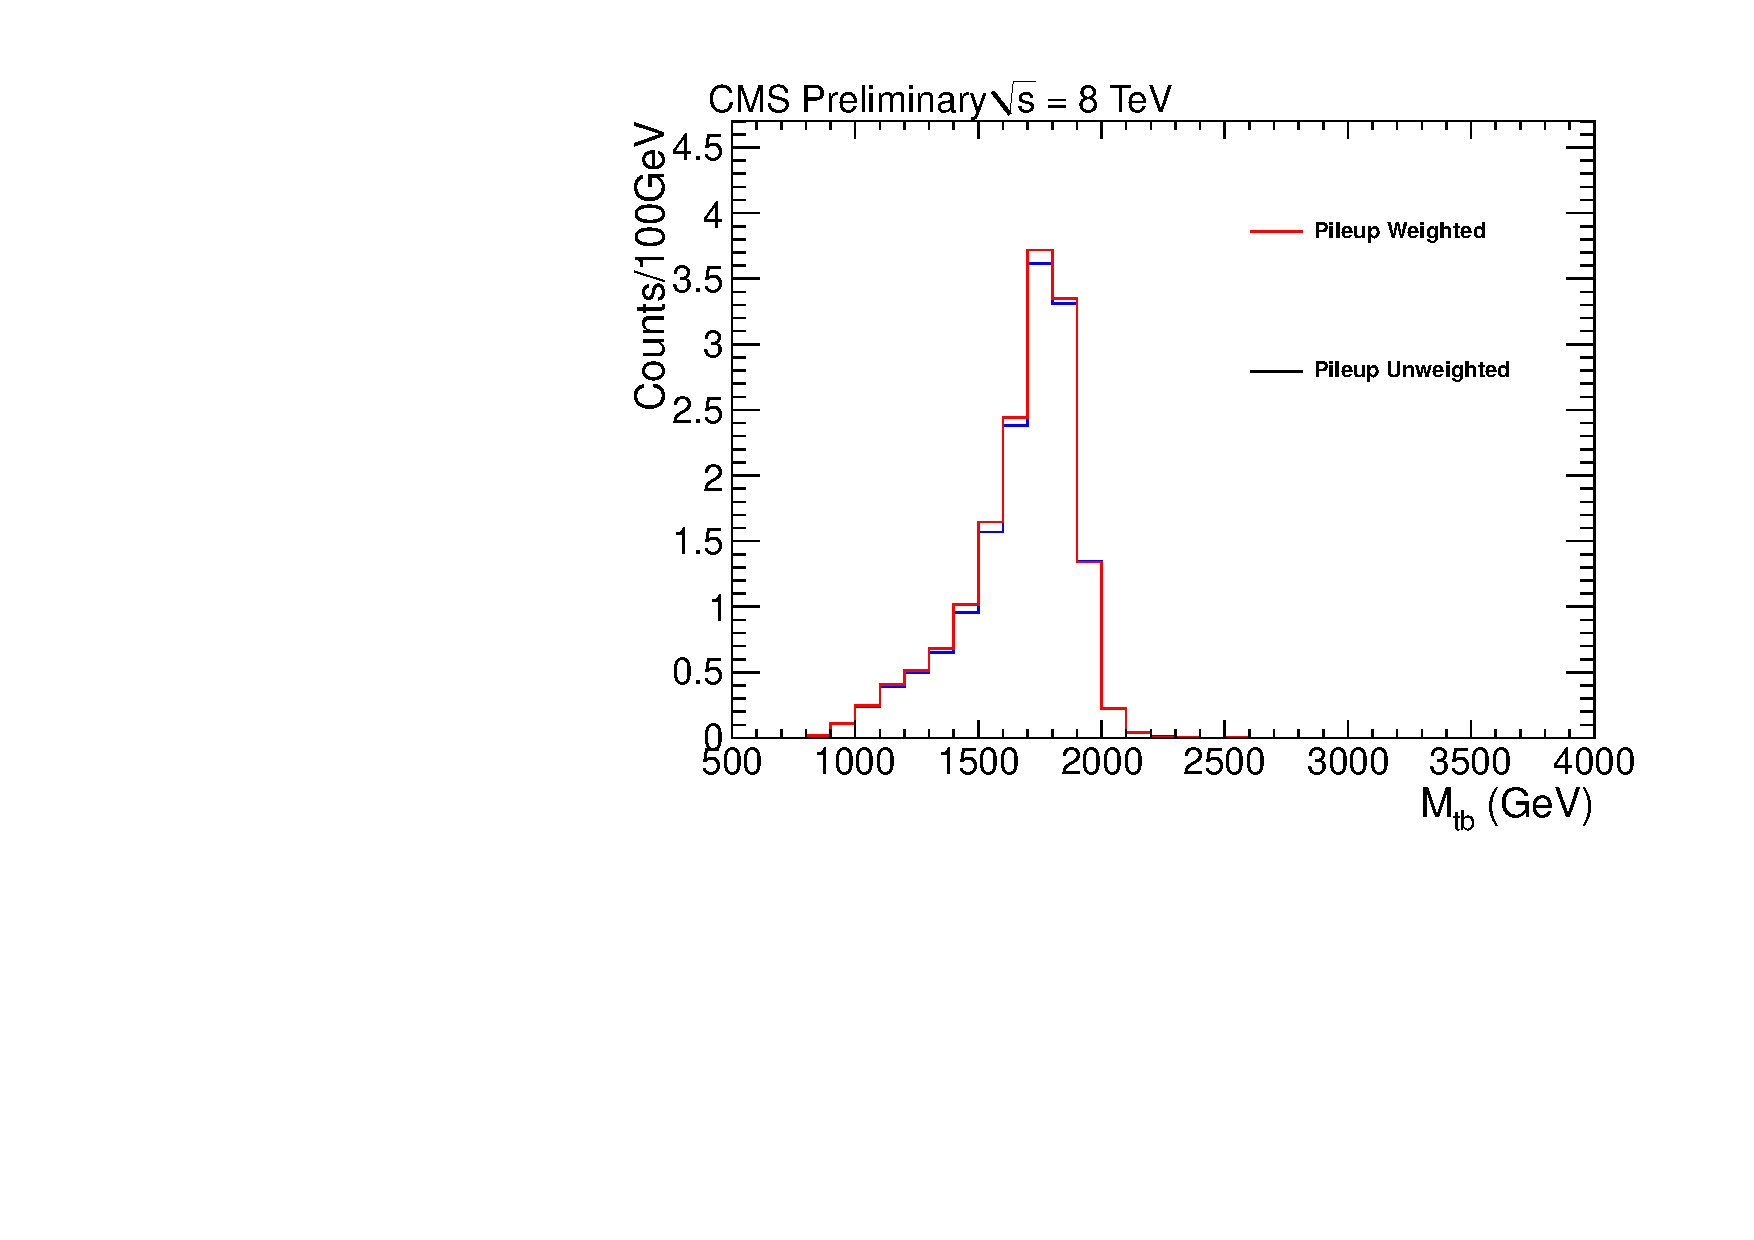
\includegraphics[width=0.9\textwidth]{AN-13-004/figs/Signal_M1900_PileupComp.pdf}
\caption{Effect of pileup-re-weighting on the Signal Monte Carlo.}
\label{figs:pileup3}
\end{figure}

\begin{figure}[htcb]
\centering
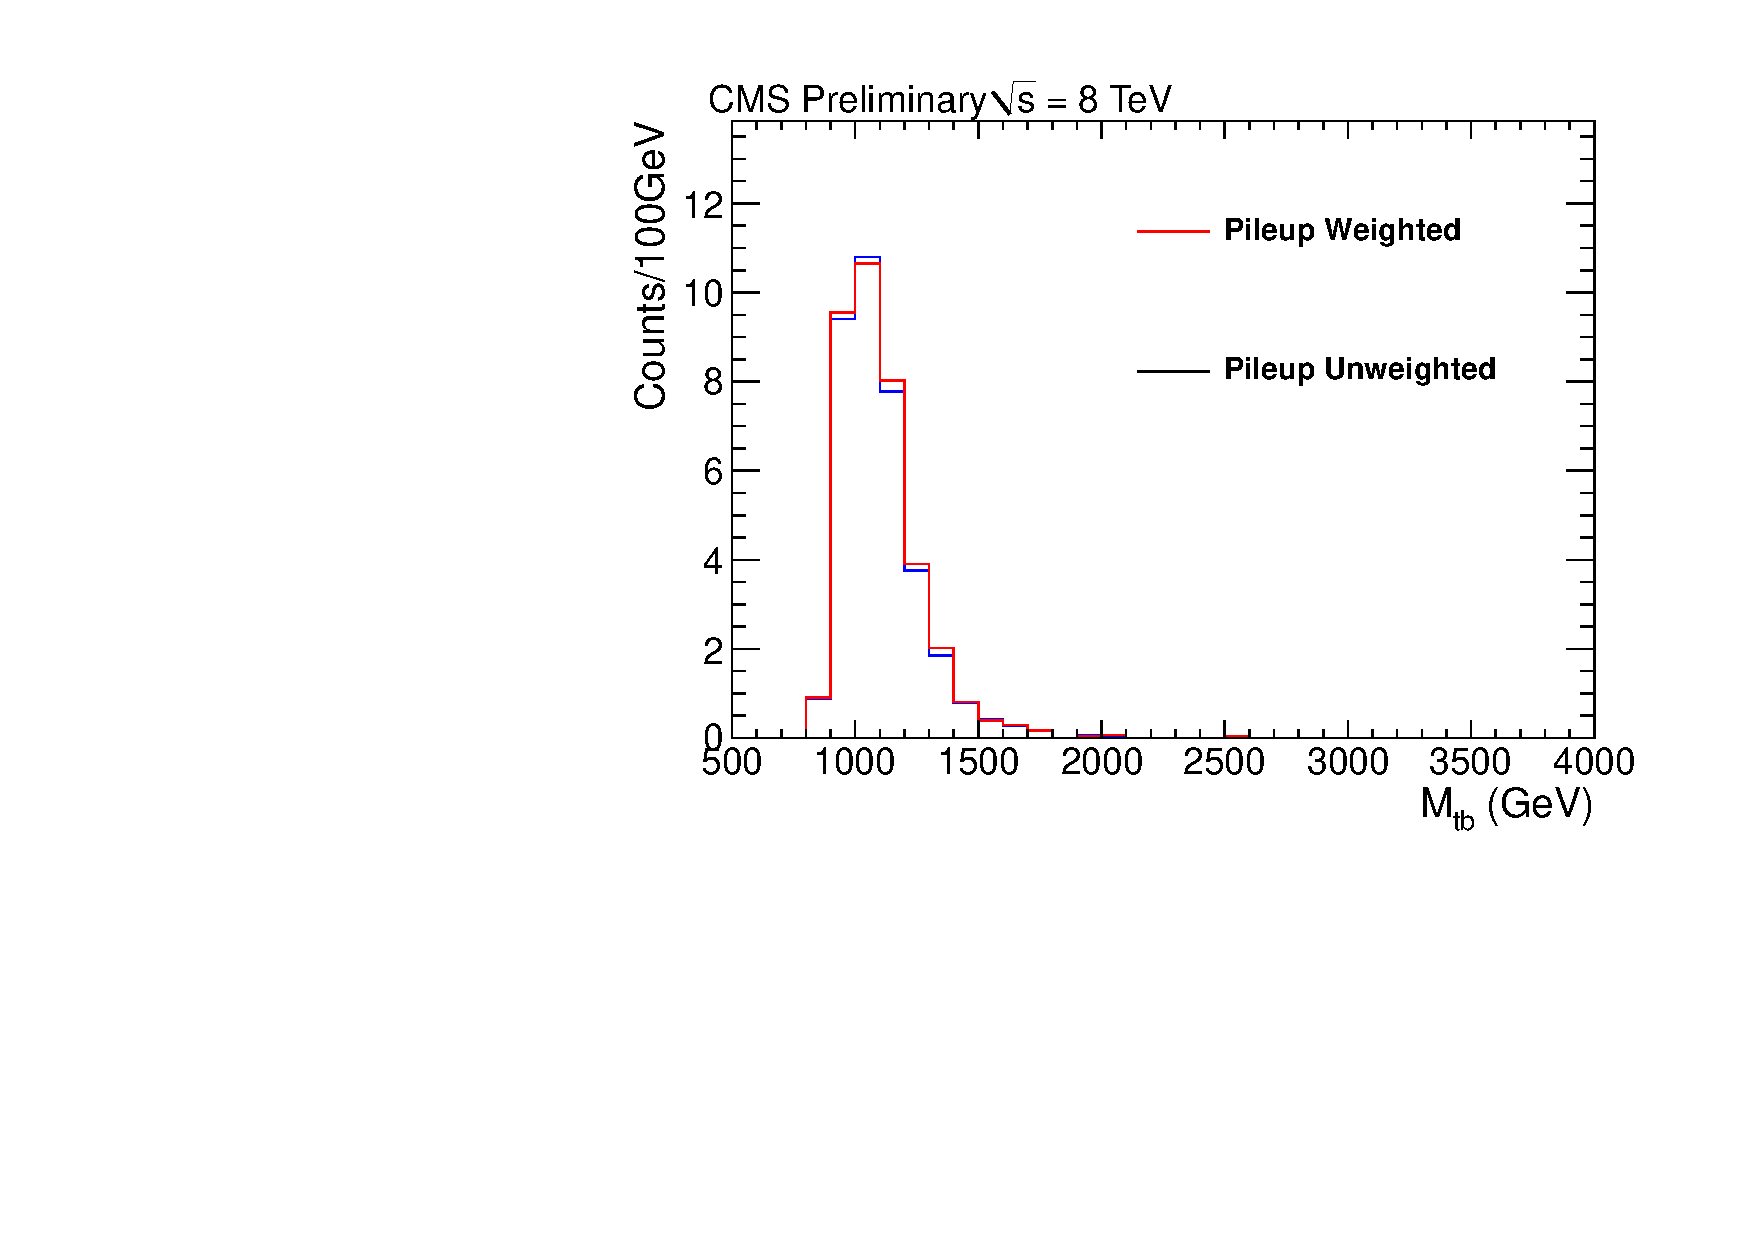
\includegraphics[width=0.9\textwidth]{AN-13-004/figs/TTbar_PileupComp.pdf}
\caption{Effect of pileup-re-weighting on the $\ttbar$ Monte Carlo.}
\label{figs:pileup3ttbar}
\end{figure}



\section{Combined CMS Top Tagging Algorithm}
\label{sec:toptagging}
\label{sec:subjetSF}

The CMS top tagging algorithm takes CA jets with $R = 0.8$ as input.  
The algorithm first attempts to decompose the CA jet into two primary subjets, and then 
performs a secondary decomposition to attempt to split the subjets into secondary subjets \cite{JME13007}.
In this process, particles with low $\pt$ or a large angular distance from the jet center are omitted.
The top tagging algorithm is based on the following cuts

\begin{itemize}
\item {\bf Jet Mass}  $\mathrm{\boldmath 140~\GeV < m_{\text{jet}} < 250~\GeV}$ - The mass of the CA jet is required to be consistent with the top quark mass. 
\item {\bf Number of Subjets}  $\mathrm{\boldmath N_{\text{subjets}} > 2}$ - The number of subjets found by the algorithm must be at least 3.
\item {\bf Minimum Pairwise Mass} $\mathrm{\boldmath m_{\text{min}} > 50~\GeV}$  - The three highest $\pt$ subjets are
taken pairwise, and each pair's invariant mass is calculated. $m_{\text{min}}$ is the mass of the pair with the lowest invariant mass. The minimum pairwise mass must be close to the W mass.   
\end{itemize}
Figure \ref{figs:CutCompP} shows the comparison of Signal and QCD Monte Carlo for the above top tagging selection. Here, the N-subjettiness and subjet b-tagging cuts are not applied.

\begin{figure}[htb]
\centering
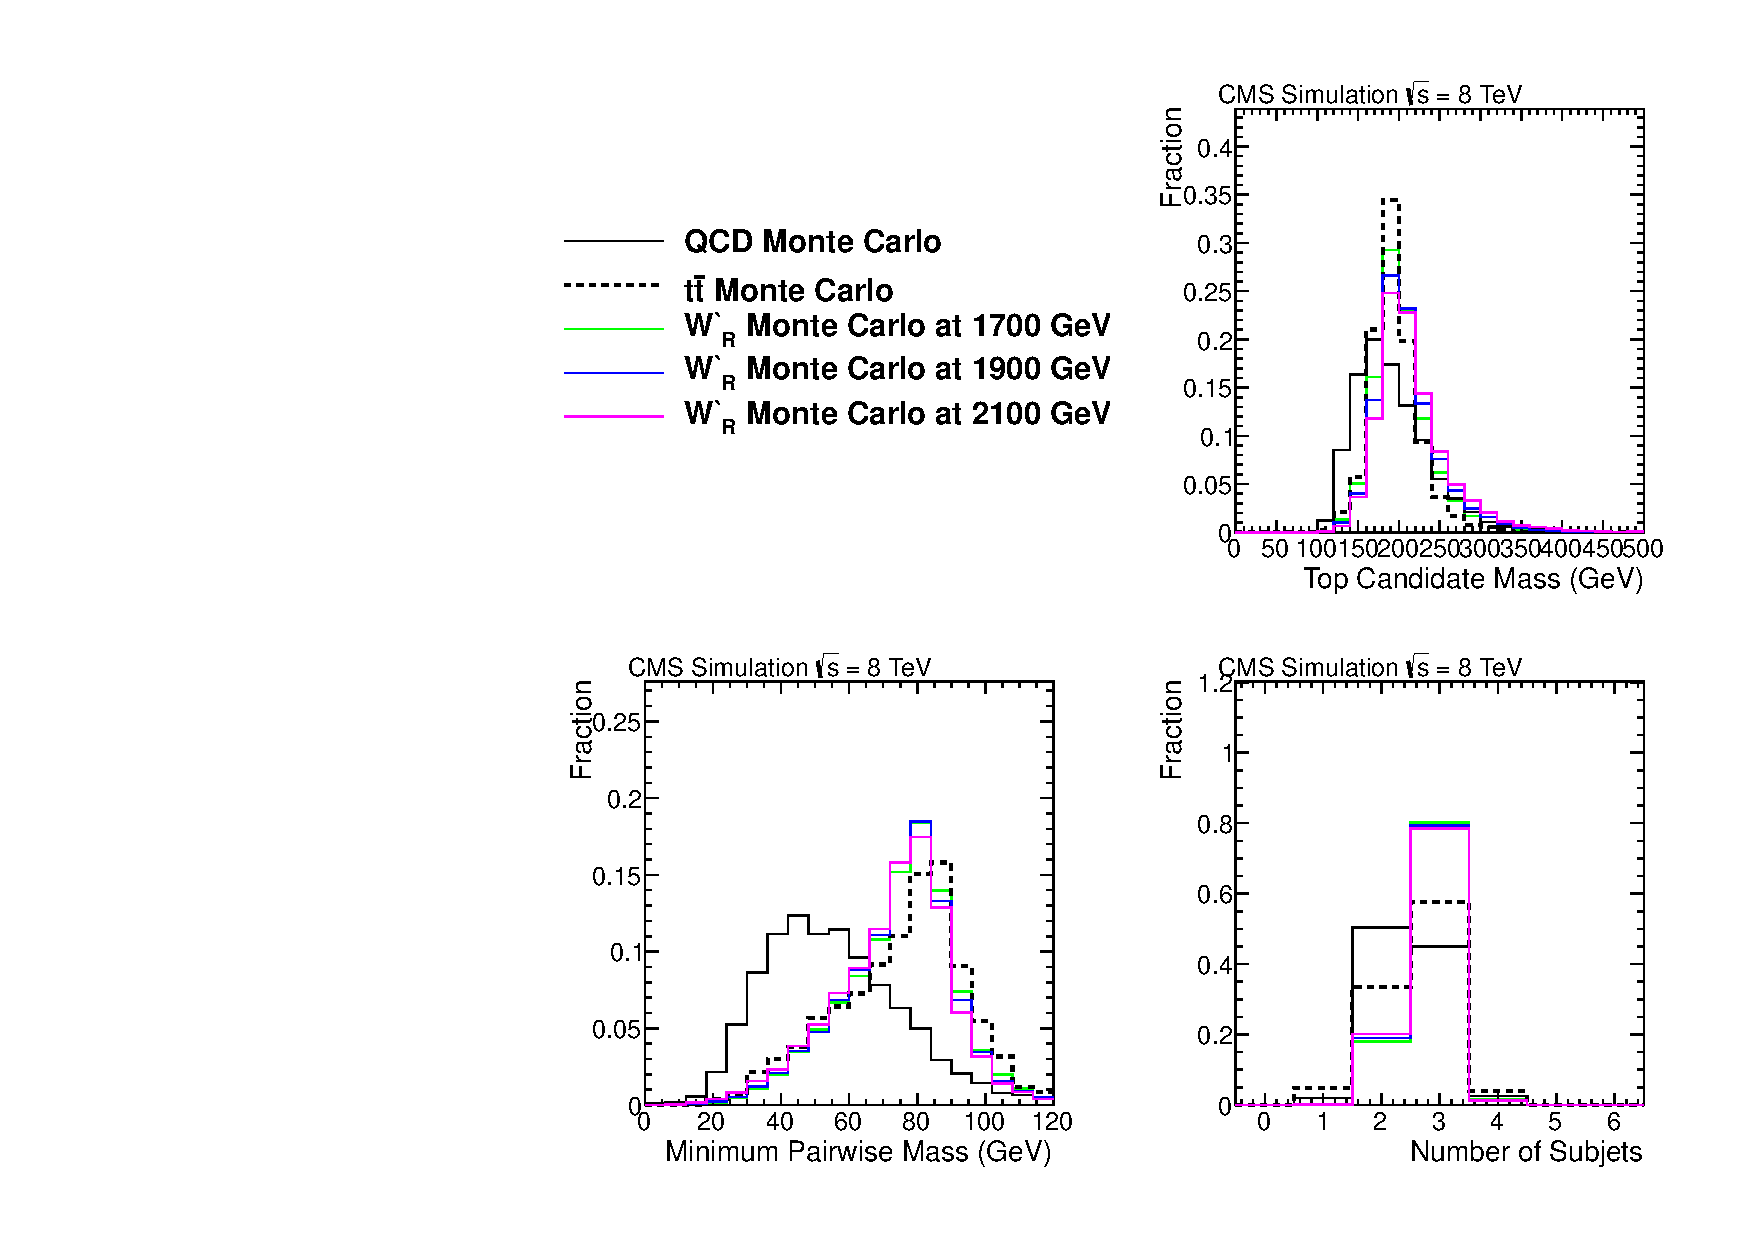
\includegraphics[width=1.0\textwidth]{AN-13-004/figs/CutCompqcdandsignal}
\caption{Comparison of the top Jet Mass, Number of Subjets, and Minimum Pairwise Mass in Signal and QCD Monte Carlo.  The cms top tagging selection is applied 
with the exception of the variable being plotted.}
\label{figs:CutCompP}
\end{figure}

The N-subjettiness algorithm can be used for boosted top jet identification \cite{Thaler:2011gf}.  N-subjettiness defines $\tau_N$ variables as follows 
\begin{eqnarray}
	\tau_{N} = \frac{1}{d_0}\sum_{i}p_{T_i}min\{\Delta R_{1,i},\Delta R_{2,i},...,\Delta R_{N,i}\}
\end{eqnarray}
where $\Delta R_{J,i}$ is between the subjet candidate and a constituent particle.  $d_0$ is a normalization factor 
\begin{eqnarray}
	d_0 = \sum_i p_{T_i} R_0
\end{eqnarray}
where $R_0$ is the characteristic jet radius used by the jet clustering algorithm.  For this analysis we use the one pass kt method of subjet axes minimization.  $\tau_N$ is a measure of how consistent the jet energy is with originating from N subjets. 
Additional discrimination power when using N-subjettiness variables is achieved by cutting on the ratio of two of these variables.   
Figure \ref{figs:NsubCOMP} shows $\tau_3/\tau_2$ comparison using signal and QCD Monte Carlo samples.  We use the standard operating point of $\tau_3/\tau_2 < 0.55$  \cite{JME13007} in the full selection.

\begin{figure}[htcb]
\begin{center}
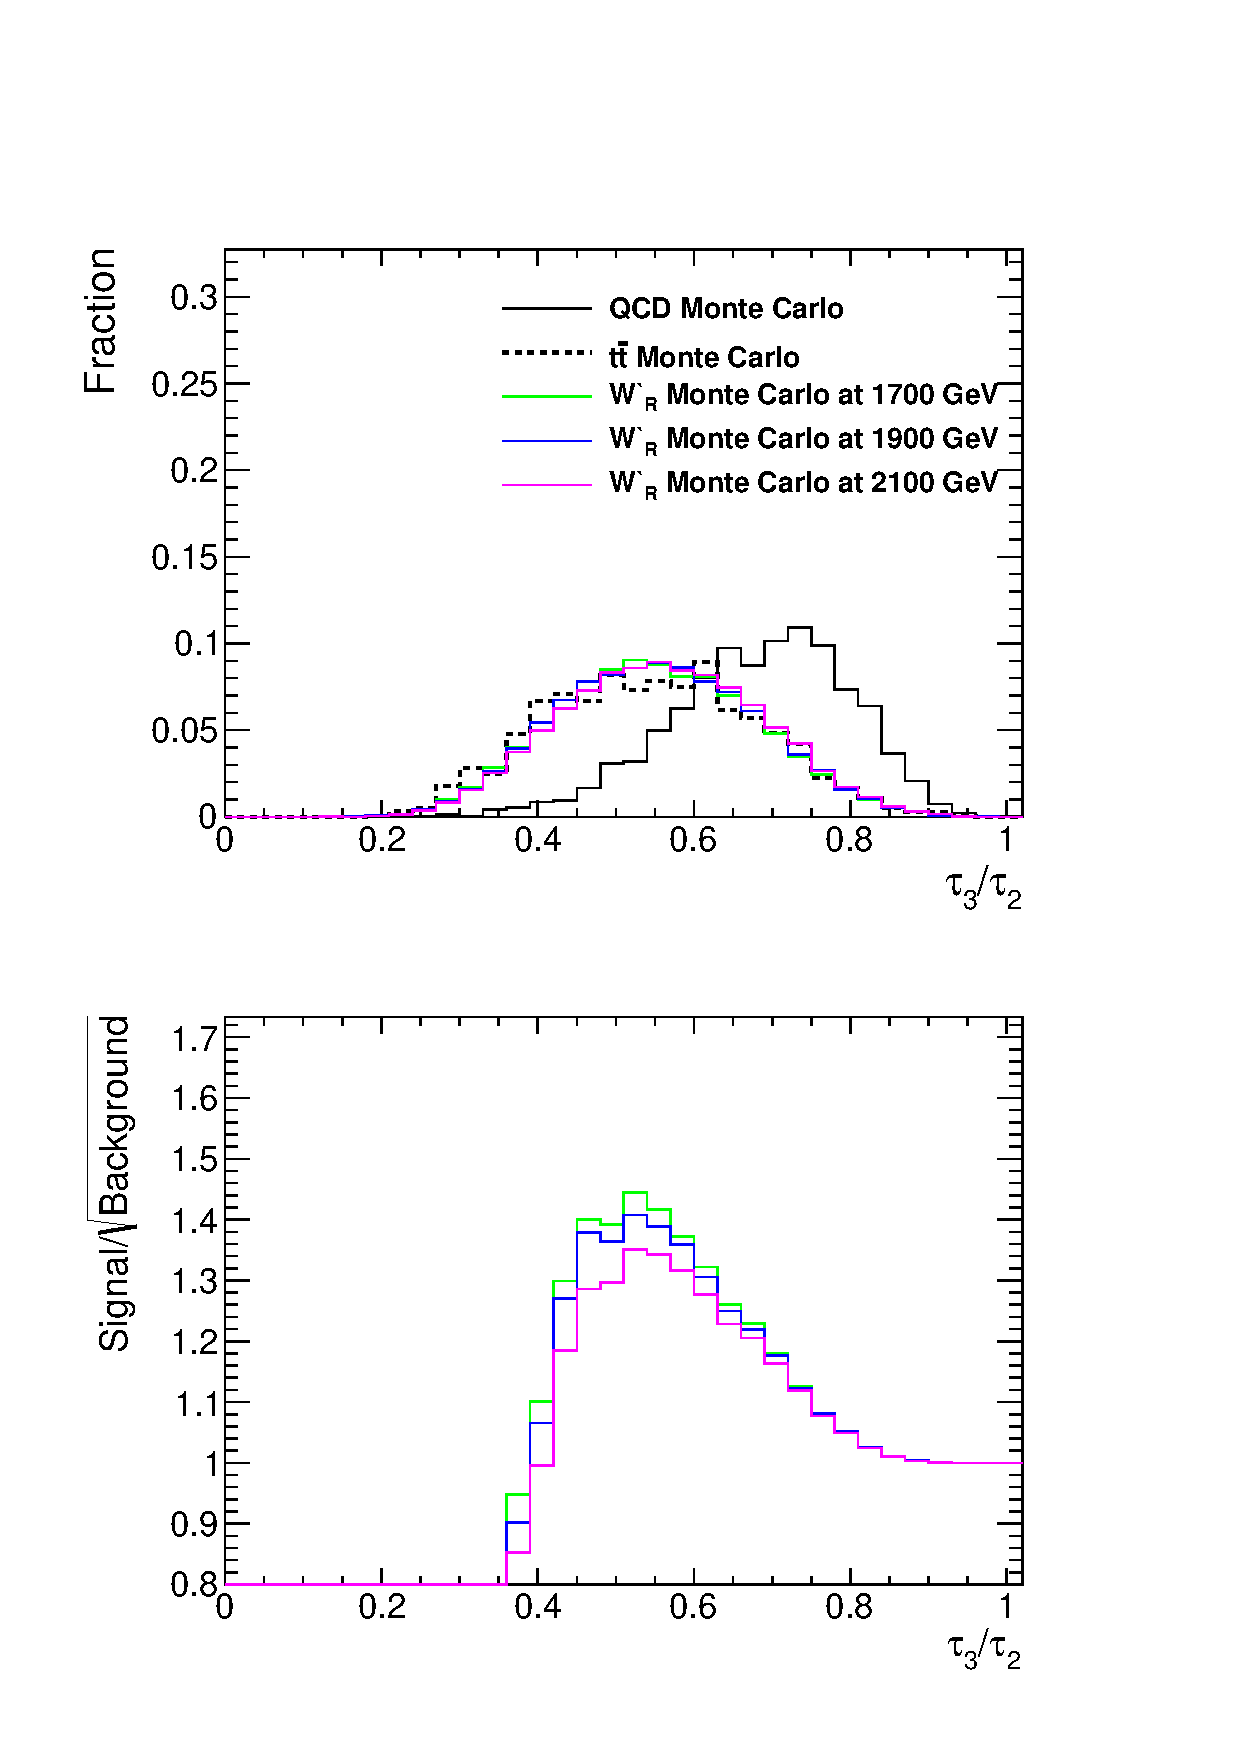
\includegraphics[width=0.7\textwidth]{AN-13-004/figs/tau32Compqcdandsignal.pdf}
\caption{
$\tau_3/\tau_2$ distributions in Signal and QCD Monte Carlo samples (top).  Plot of Signal/$\sqrt{\text{Background}}$ (bottom), derived from the top plot.
}
\label{figs:NsubCOMP}
\end{center}
\end{figure}

The use of b-tagging algorithms on subjets is described in \cite{CMS-PAS-BTV-13-001}.  We apply the Combined Secondary Vertex b-tagging algorithm 
to all of the subjets found by the CA declustering sequence described 
above.  The optimal discrimination variable when using subjet b-tagging is the maximum discriminant out of the three or four subjets found.  
Figure \ref{figs:BtagCOMP} shows the maximum subjet CSV b discriminant comparison using signal and QCD Monte Carlo samples.  We use the standard CSV working point $SJ_{\text{CSVMAX}} > 0.679$.

\begin{figure}[htcb]
\begin{center}
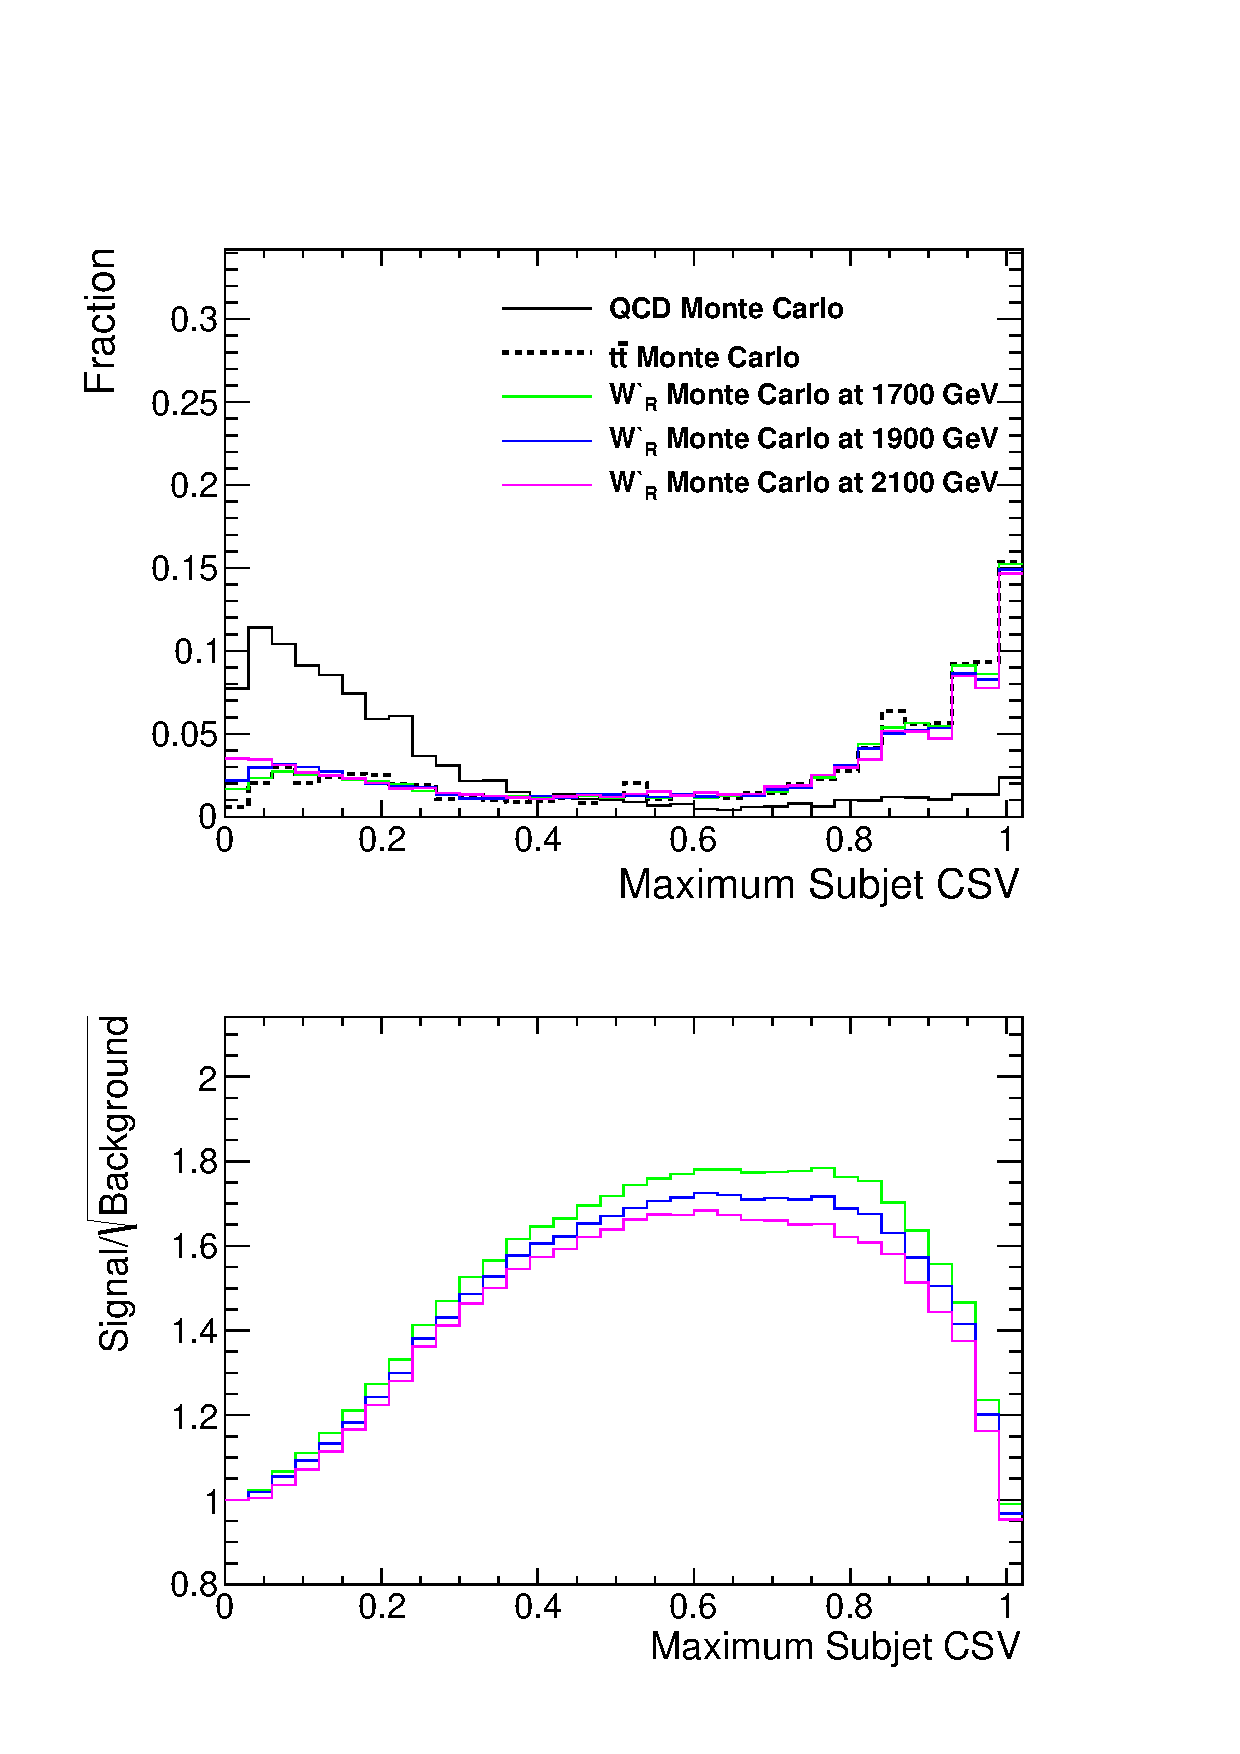
\includegraphics[width=0.7\textwidth]{AN-13-004/figs/bmaxCompqcdandsignal.pdf}
\caption{
Maximum subjet CSV distributions in Signal and QCD Monte Carlo samples (top).  Plot of Signal/$\sqrt{\text{Background}}$ (bottom), derived from the top plot. 
}
\label{figs:BtagCOMP}
\end{center}
\end{figure}

Substructure variables in the signal region have known differences in data and Monte Carlo \cite{JME13007}.  
We use the top tagging scale factor with the addition of subjet b-tagging and N-subjettiness discrimination that is extracted 
from efficiency comparisons of data and Monte Carlo in a highly pure semileptonic $\ttbar$ sample.   
The scale factor for this effect is 1.04 and is applied to the signal Monte Carlo samples used in the main analysis.  
There is a 13\% uncertainty on this scale factor which is purely statistical, as the study is dominated by statistical uncertainty.  
The scale factor is obtained from the plots shown in Figure \ref{figs:type1_topmasspowheg}.

\begin{figure}
\begin{center}
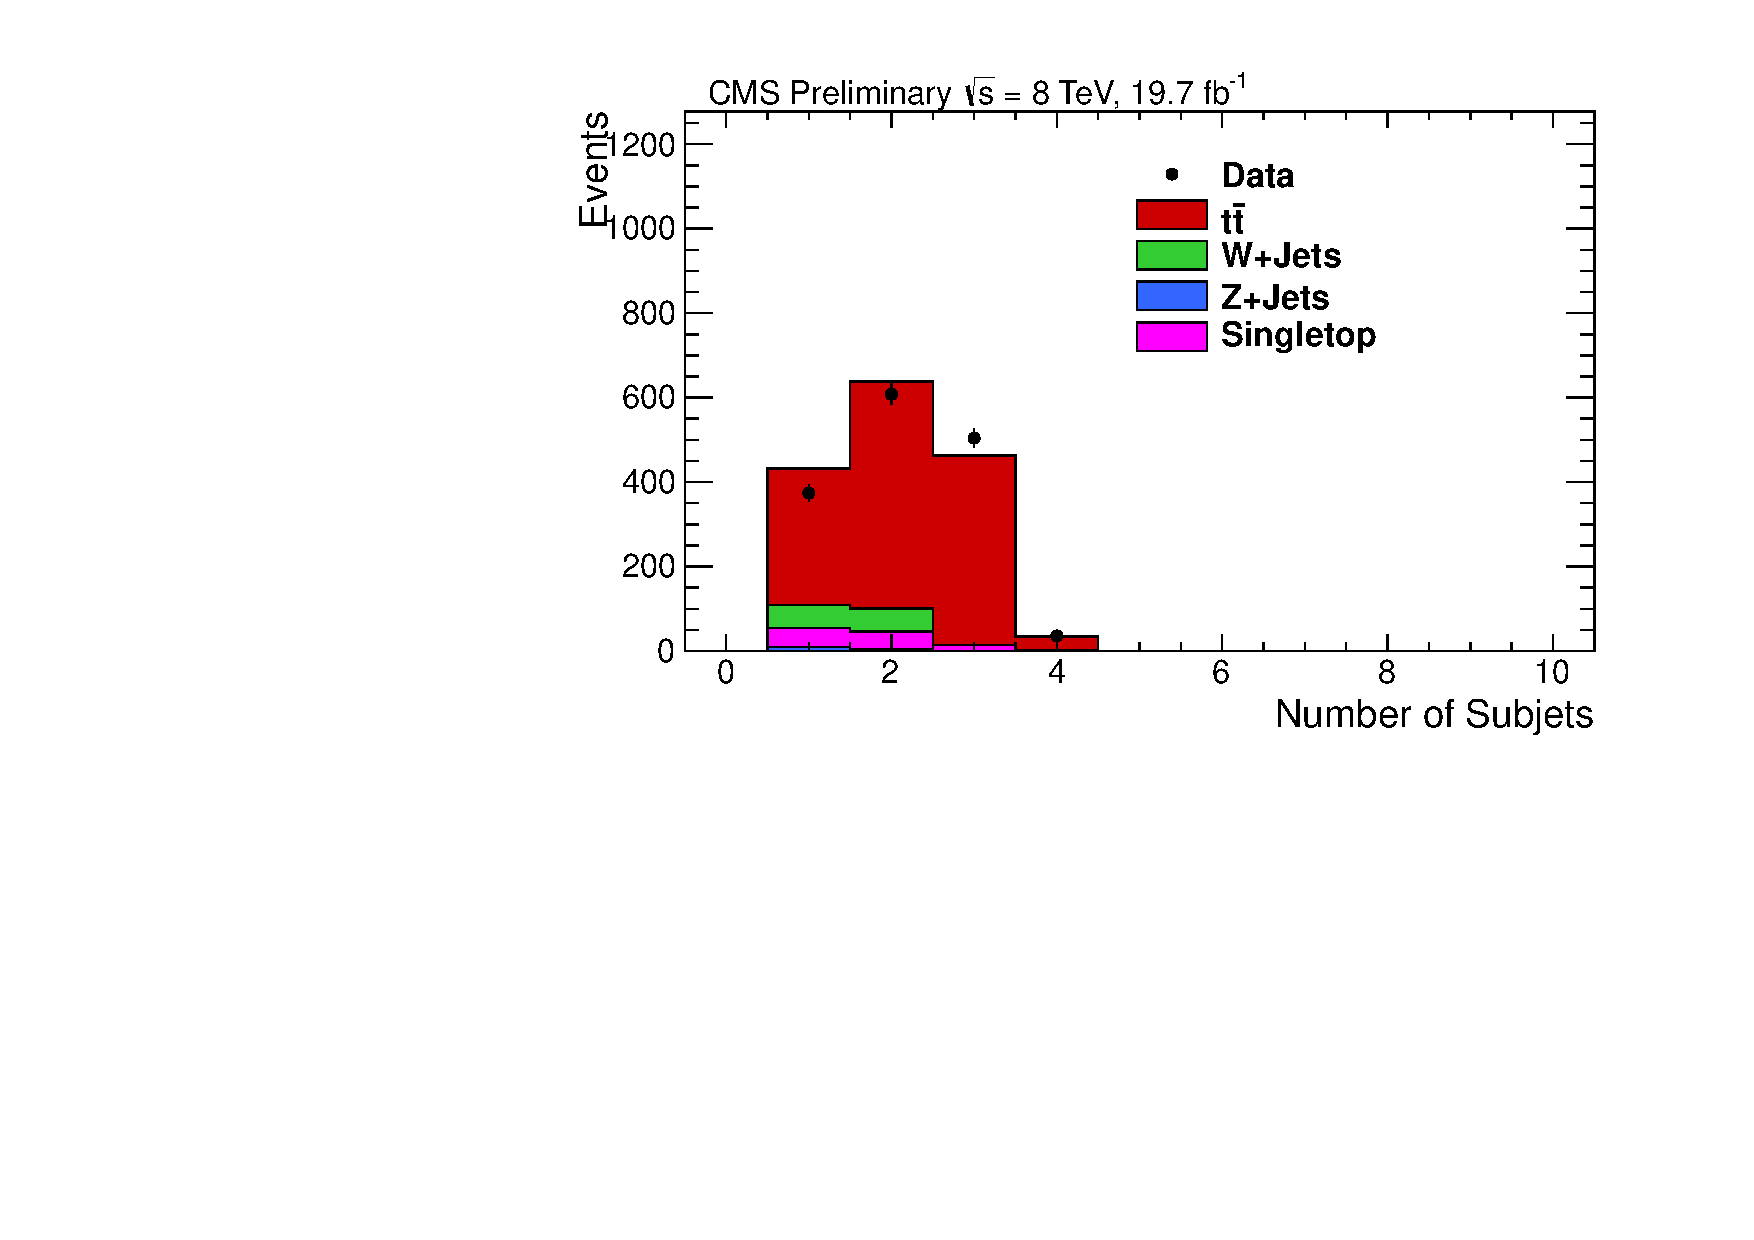
\includegraphics[width=0.45\linewidth]{AN-13-004/figs/semiLepMass_t1Nsubjets_POWHEG_TTWeight.pdf}
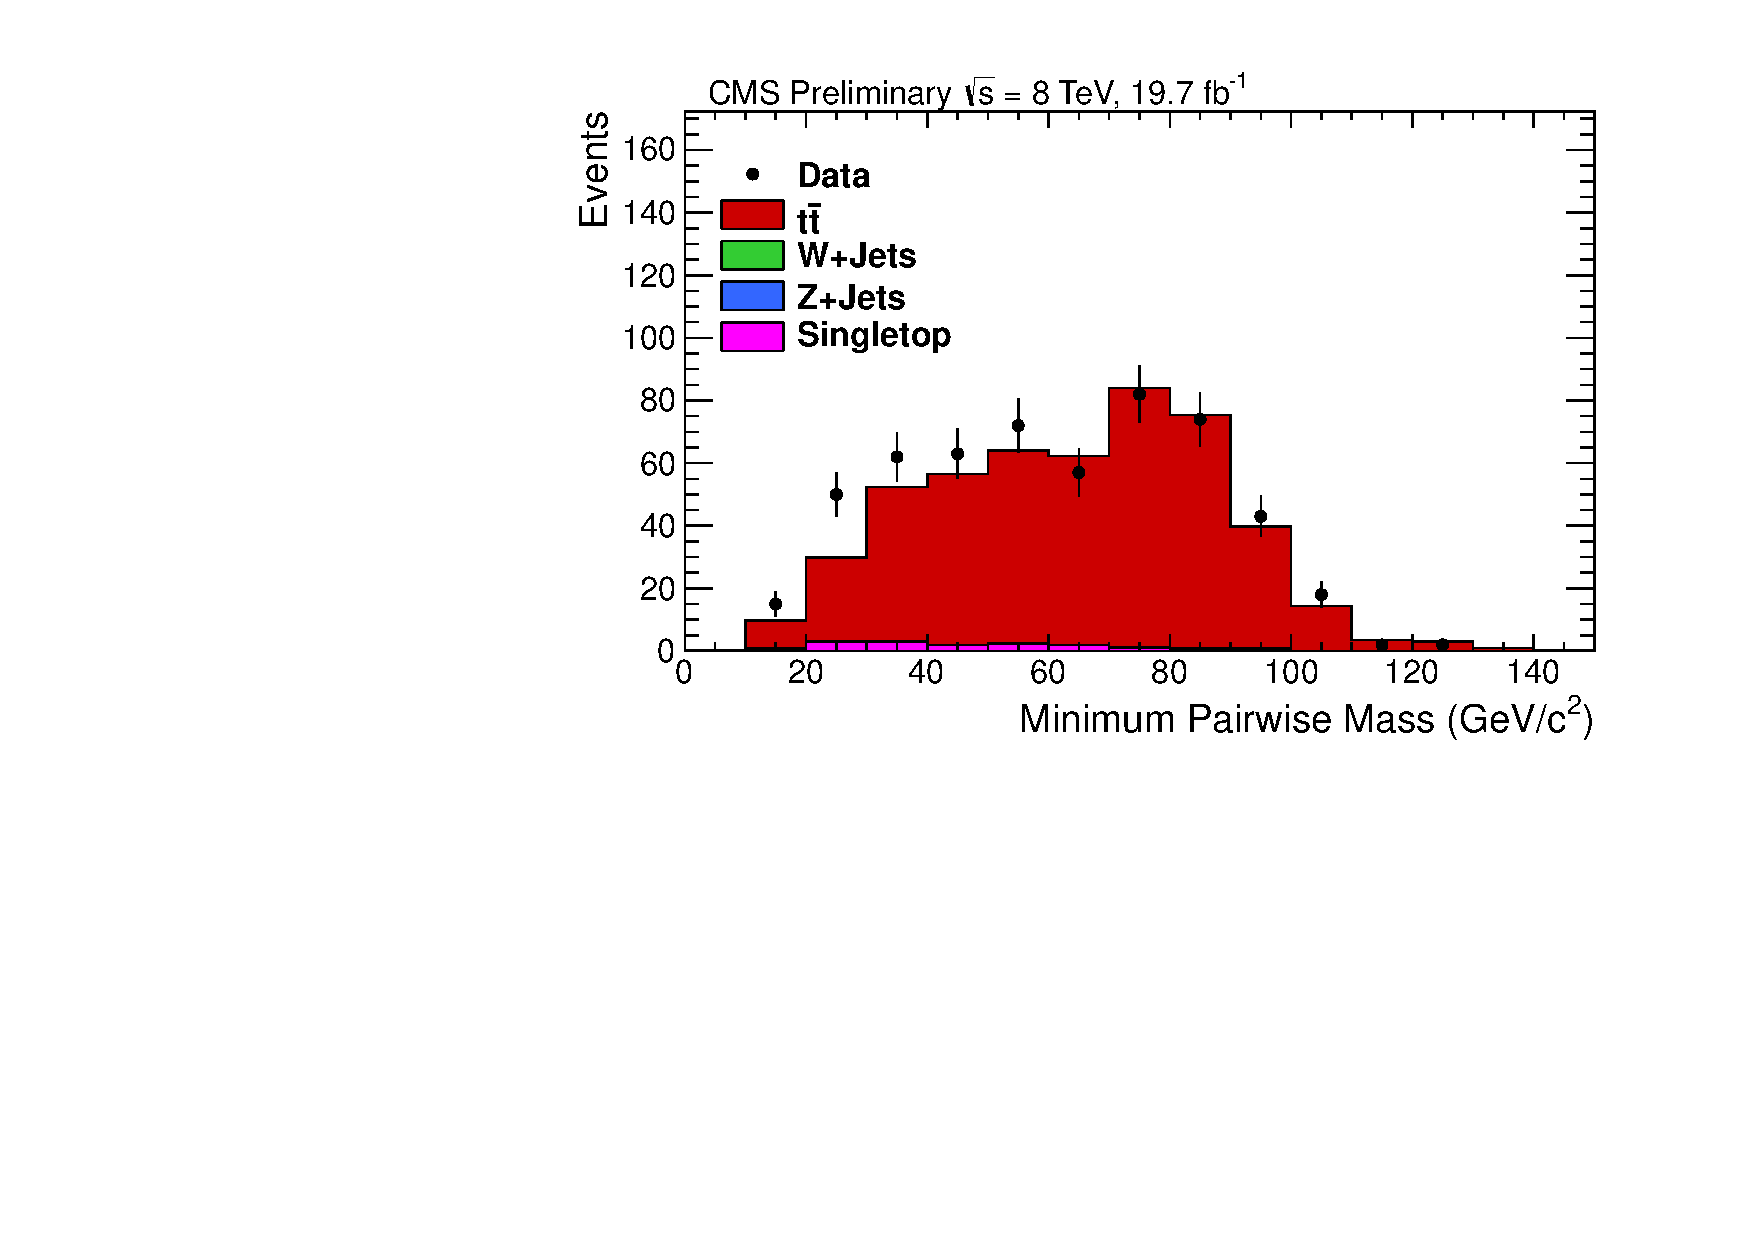
\includegraphics[width=0.45\linewidth]{AN-13-004/figs/semiLepMass_t1MinimumPairwiseMass_POWHEG_TTWeight.pdf}\\
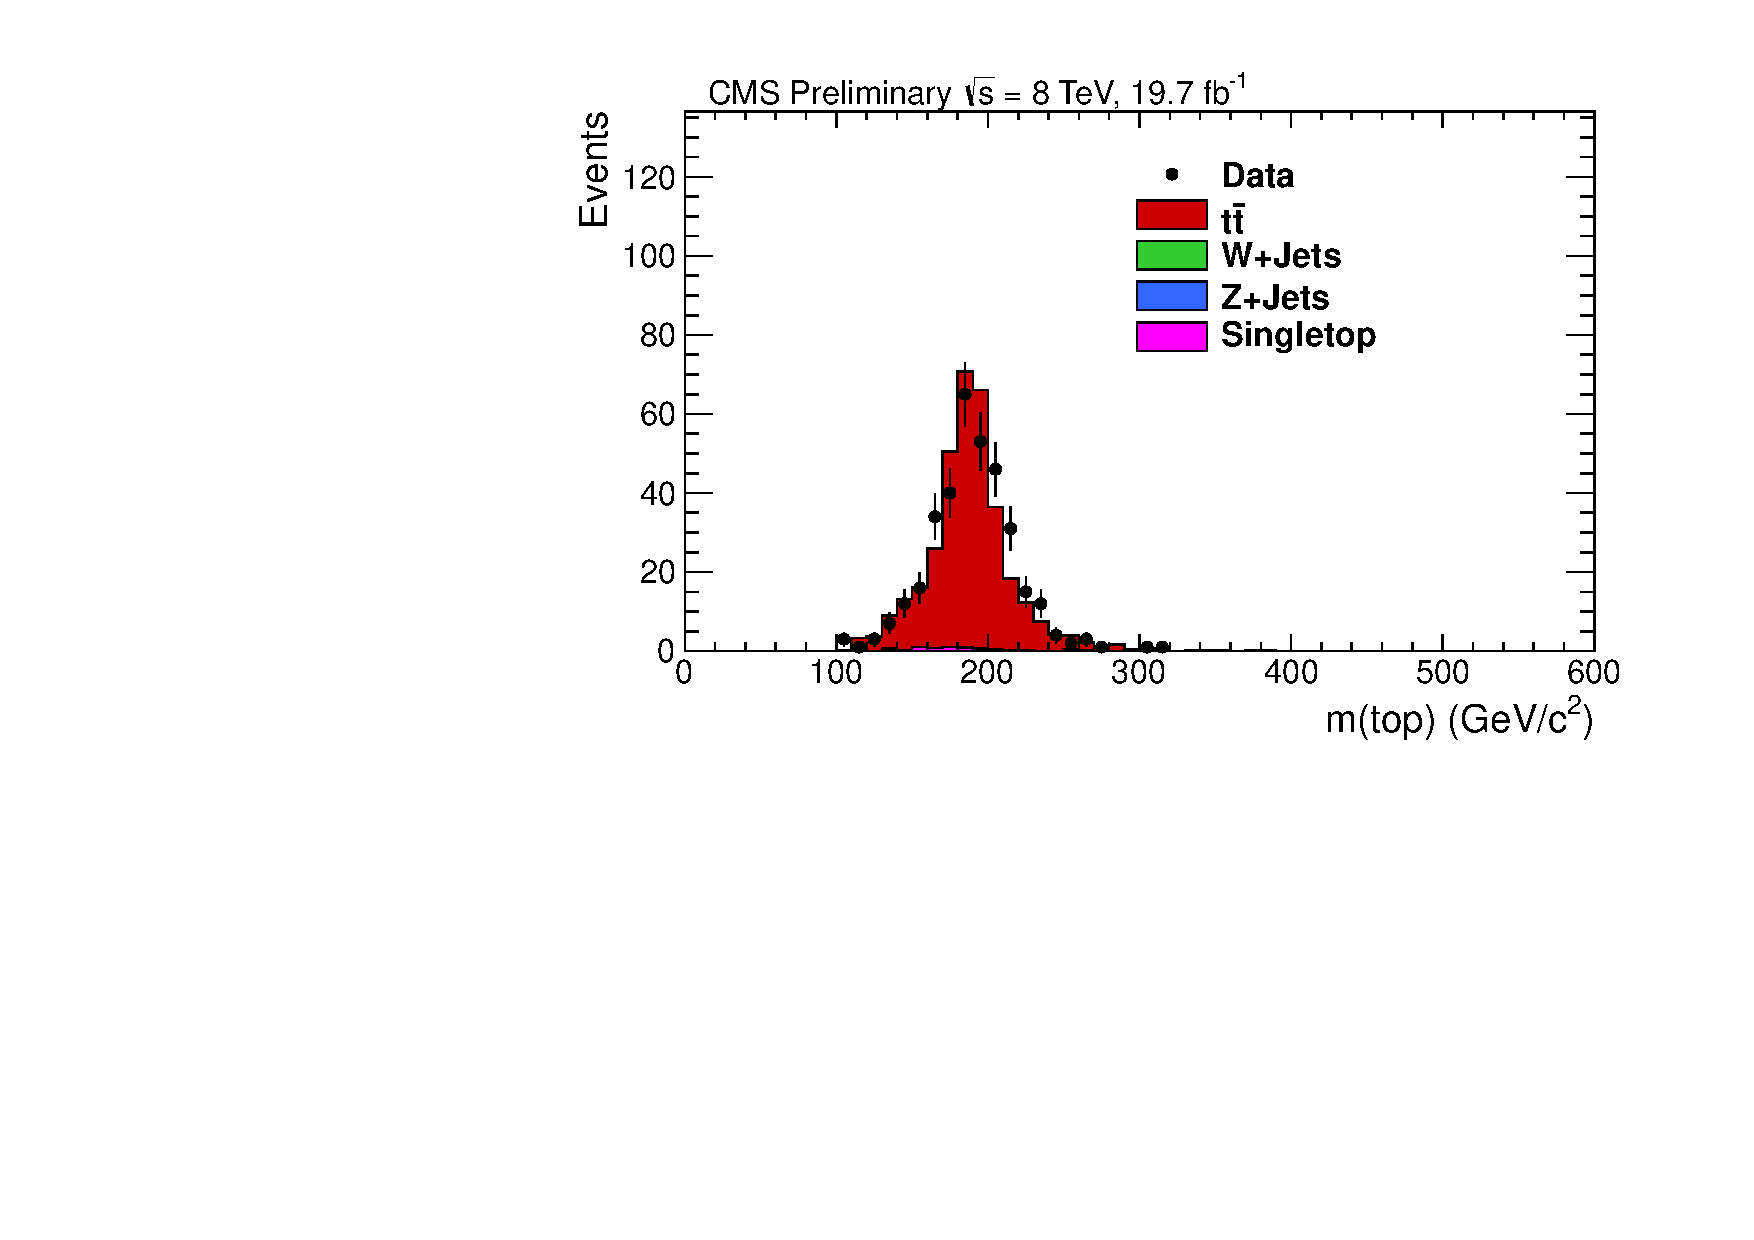
\includegraphics[width=0.45\linewidth]{AN-13-004/figs/semiLepMass_t1TopMass_POWHEG_TTWeight.pdf}
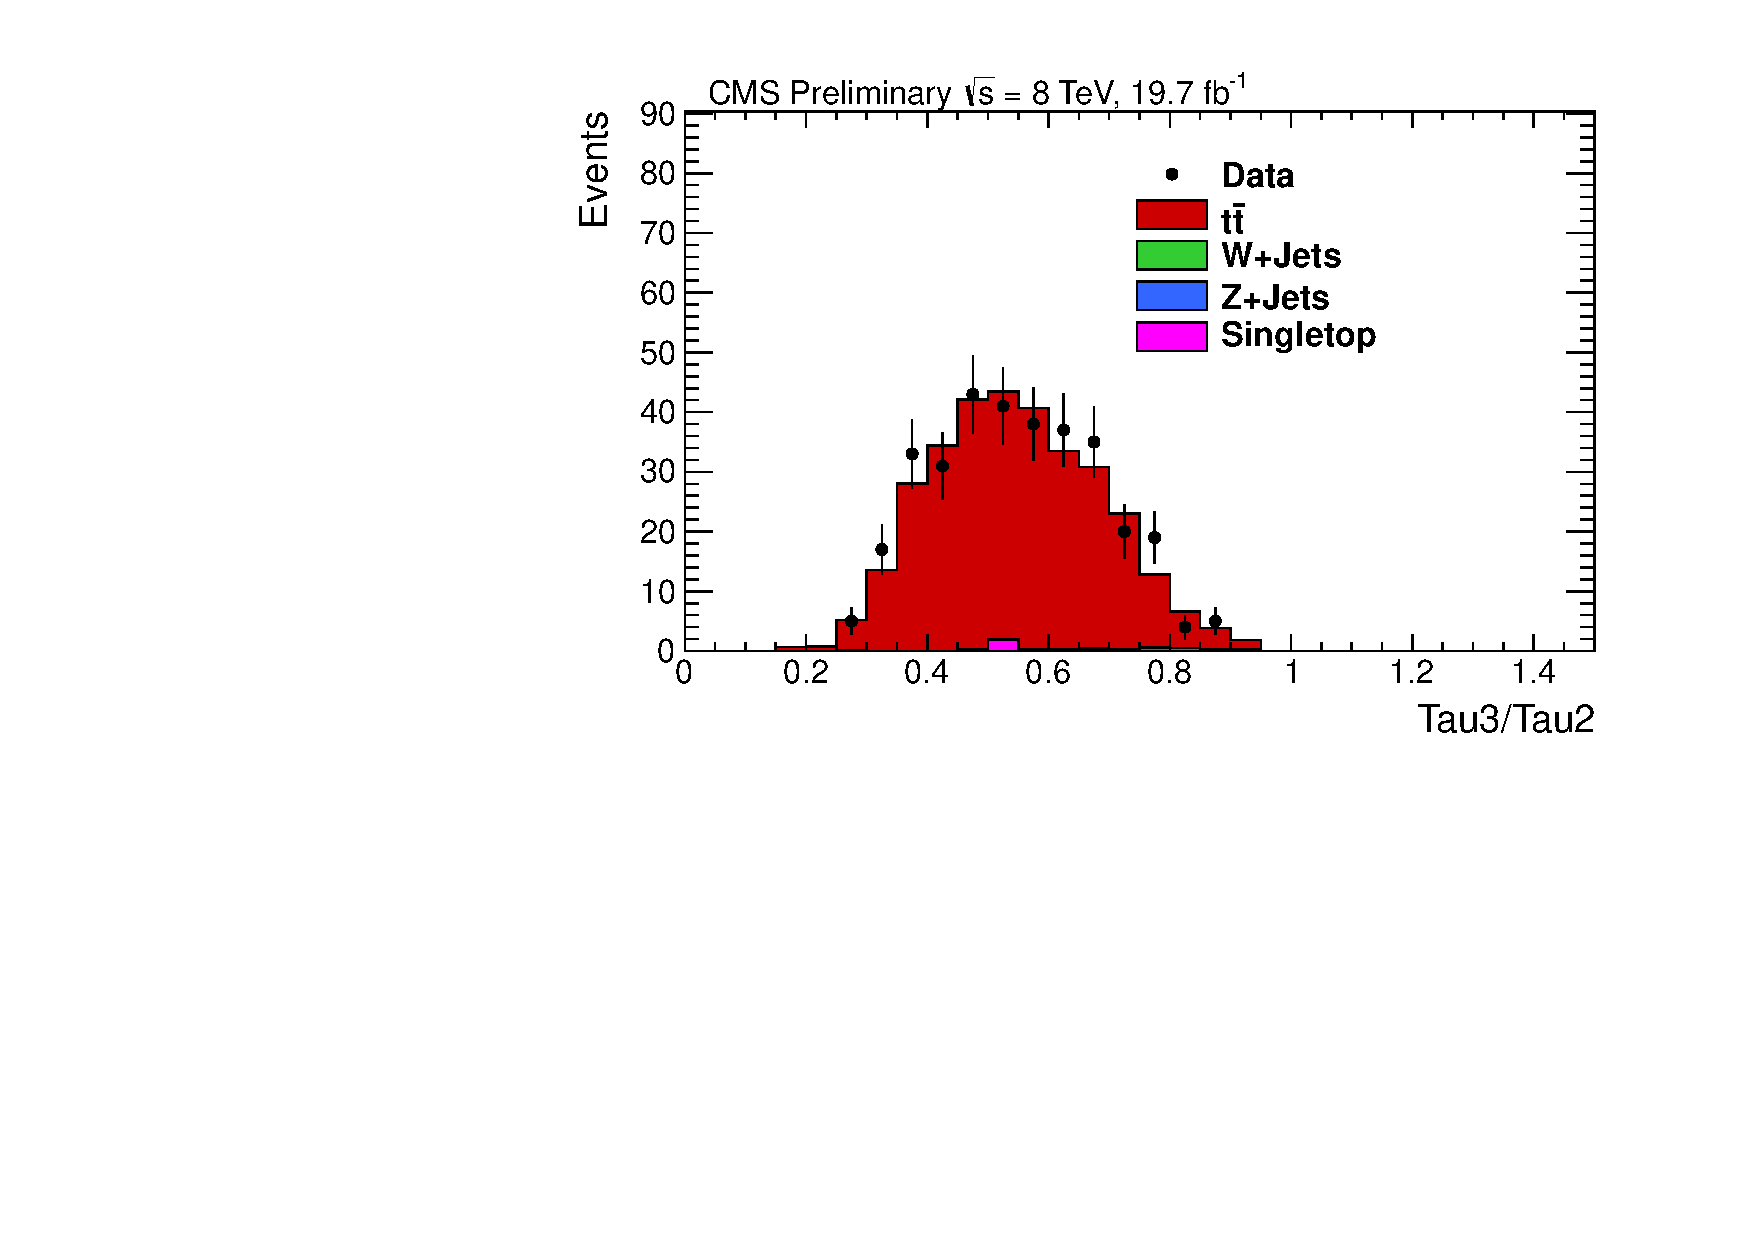
\includegraphics[width=0.45\linewidth]{AN-13-004/figs/semiLepMass_t1Tau32_POWHEG_TTWeight.pdf}\\
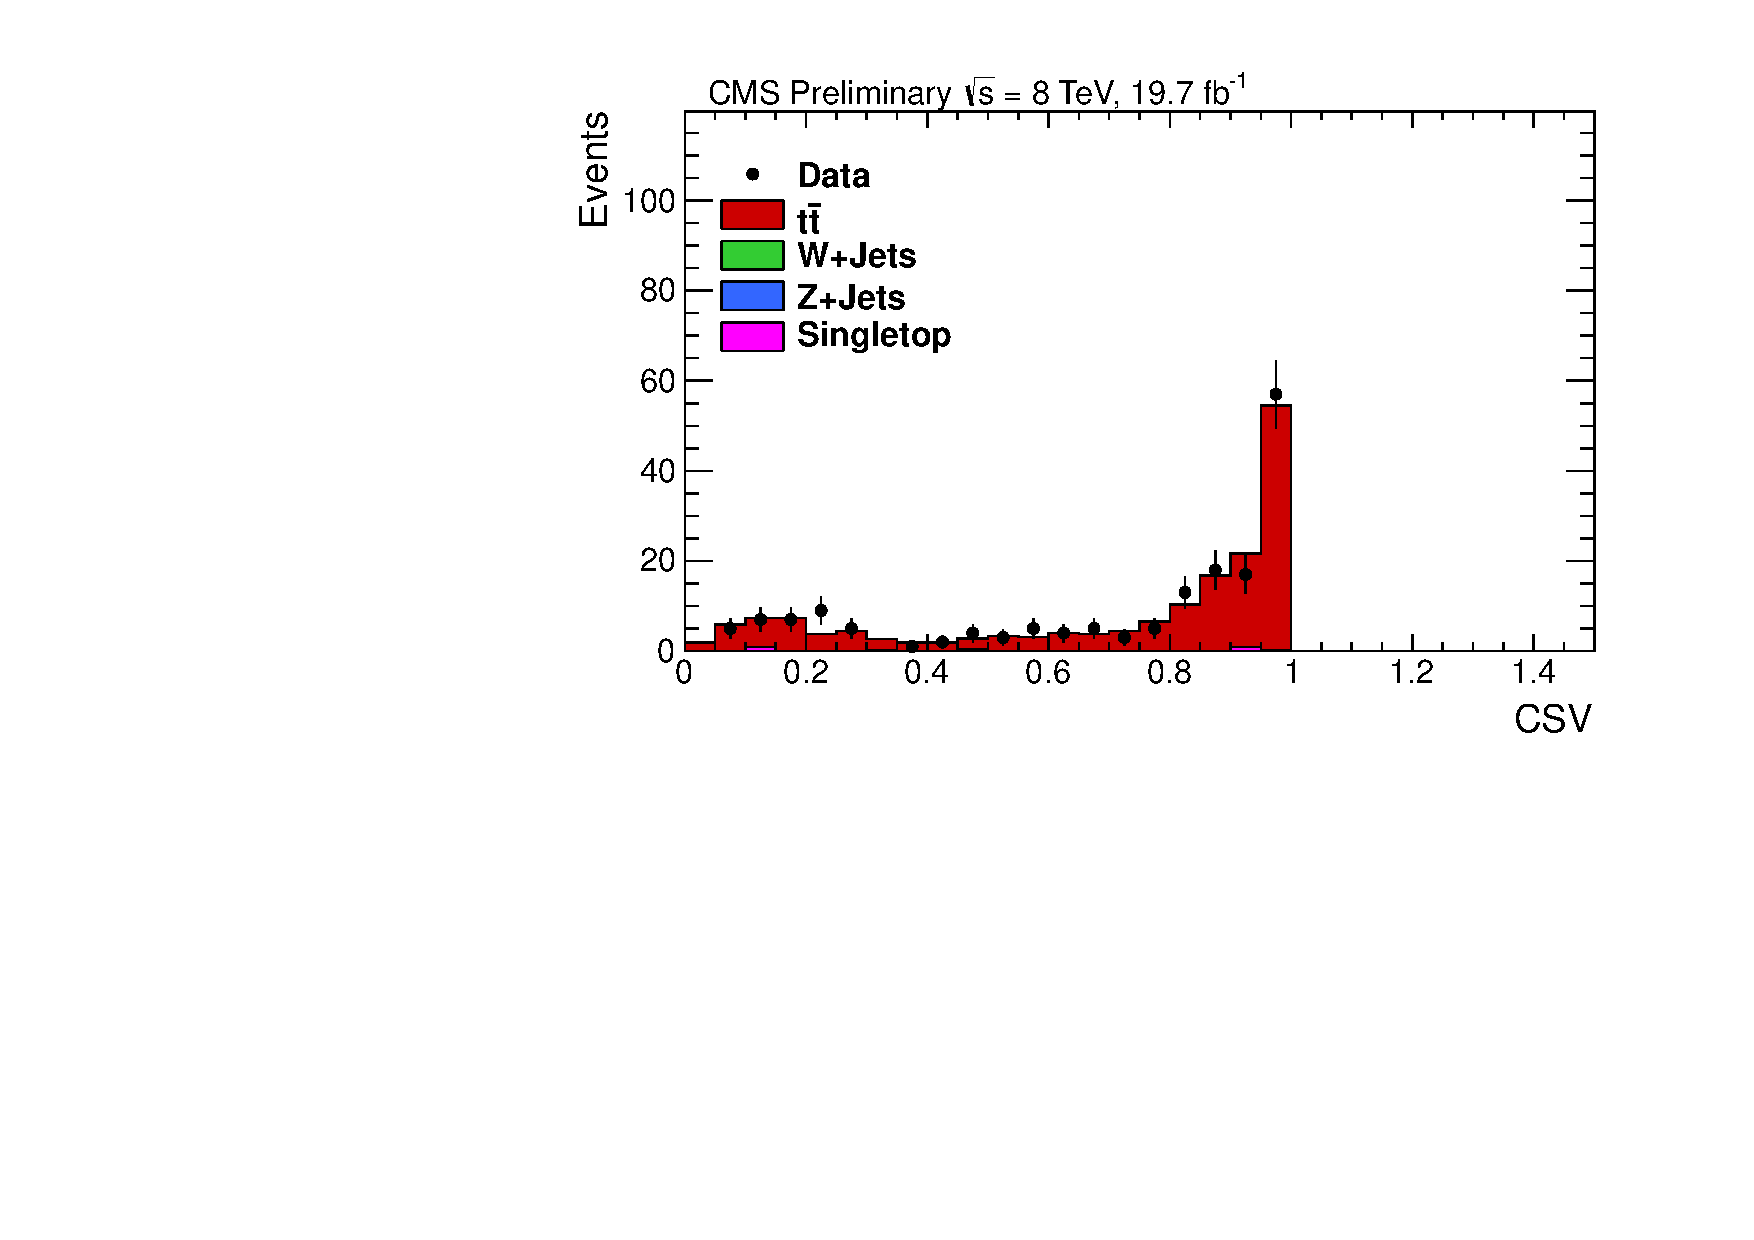
\includegraphics[width=0.45\linewidth]{AN-13-004/figs/semiLepMass_t1BMax_POWHEG_TTWeight.pdf}
\end{center}
\caption{ a.)Number of subjets, b.)minimum pairwise subjet mass, c.)jet mass, d.)$\tau_{3}/\tau_{2}$, and  e.)maximum subjet CSV for fully-merged top candidates
  found in the semileptonic $\ttbar$ sample, used to evaluate the top-tagging efficiency SF.  These Figures are extracted using the Powheg $\ttbar$ Monte Carlo Sample. }%  The shaded regions represent the total uncertainty on the background model.}
\label{figs:type1_topmasspowheg}
\end{figure}

\section{Delta Rapidity Cut}
\label{sec:deltarapidity}
At high $M_{\tbbar}$, jets that originate from QCD multijet production are widely separated in rapidity (high $\Delta y$).
However the jets originating from a high mass $\tbbar$ resonance do not exhibit such pronounced separation.  The effect is not pronounced over the entire 
$M_{\tbbar}$ spectrum, but for high values of $M_{\tbbar}$ the analysis can achieve greater separation of signal and background.  We therefore place a cut on $|\Delta y| < 1.6$ 
for the full selection.  The value for this cut was chosen by investigating the Signal/$\sqrt{\text{Background}}$ distribution in events that have $M_{\tbbar}>2000~\GeV$.  
Because it is not as effective over the entire $M_{\tbbar}$ range, the value is set slightly off the peak to minimize loss of signal efficiency.
%The value of 1.6 was determined by optimizing $S/\sqrt{B}$ where $S$ is the number of events in the signal region and $B$ is the number of events attributed to background in the region of interest for each signal mass point.  The cut value was chosen based on maximizing the expected counting experiment limit described in Section \ref{sec:countingexperiment}.  
Figure \ref{figs:CutComp} shows the comparison of $|\Delta y|$ for high $M_{\tbbar}$ in signal and QCD MC.  
Here, the N-subjettiness and subjet b-tagging cuts are not applied.
% Additionally, the lowest $\pt$ QCD MC sample has poor statistics for the high $M_{tb}$ region and is not included in this figure.

\begin{figure}[htb]
\centering
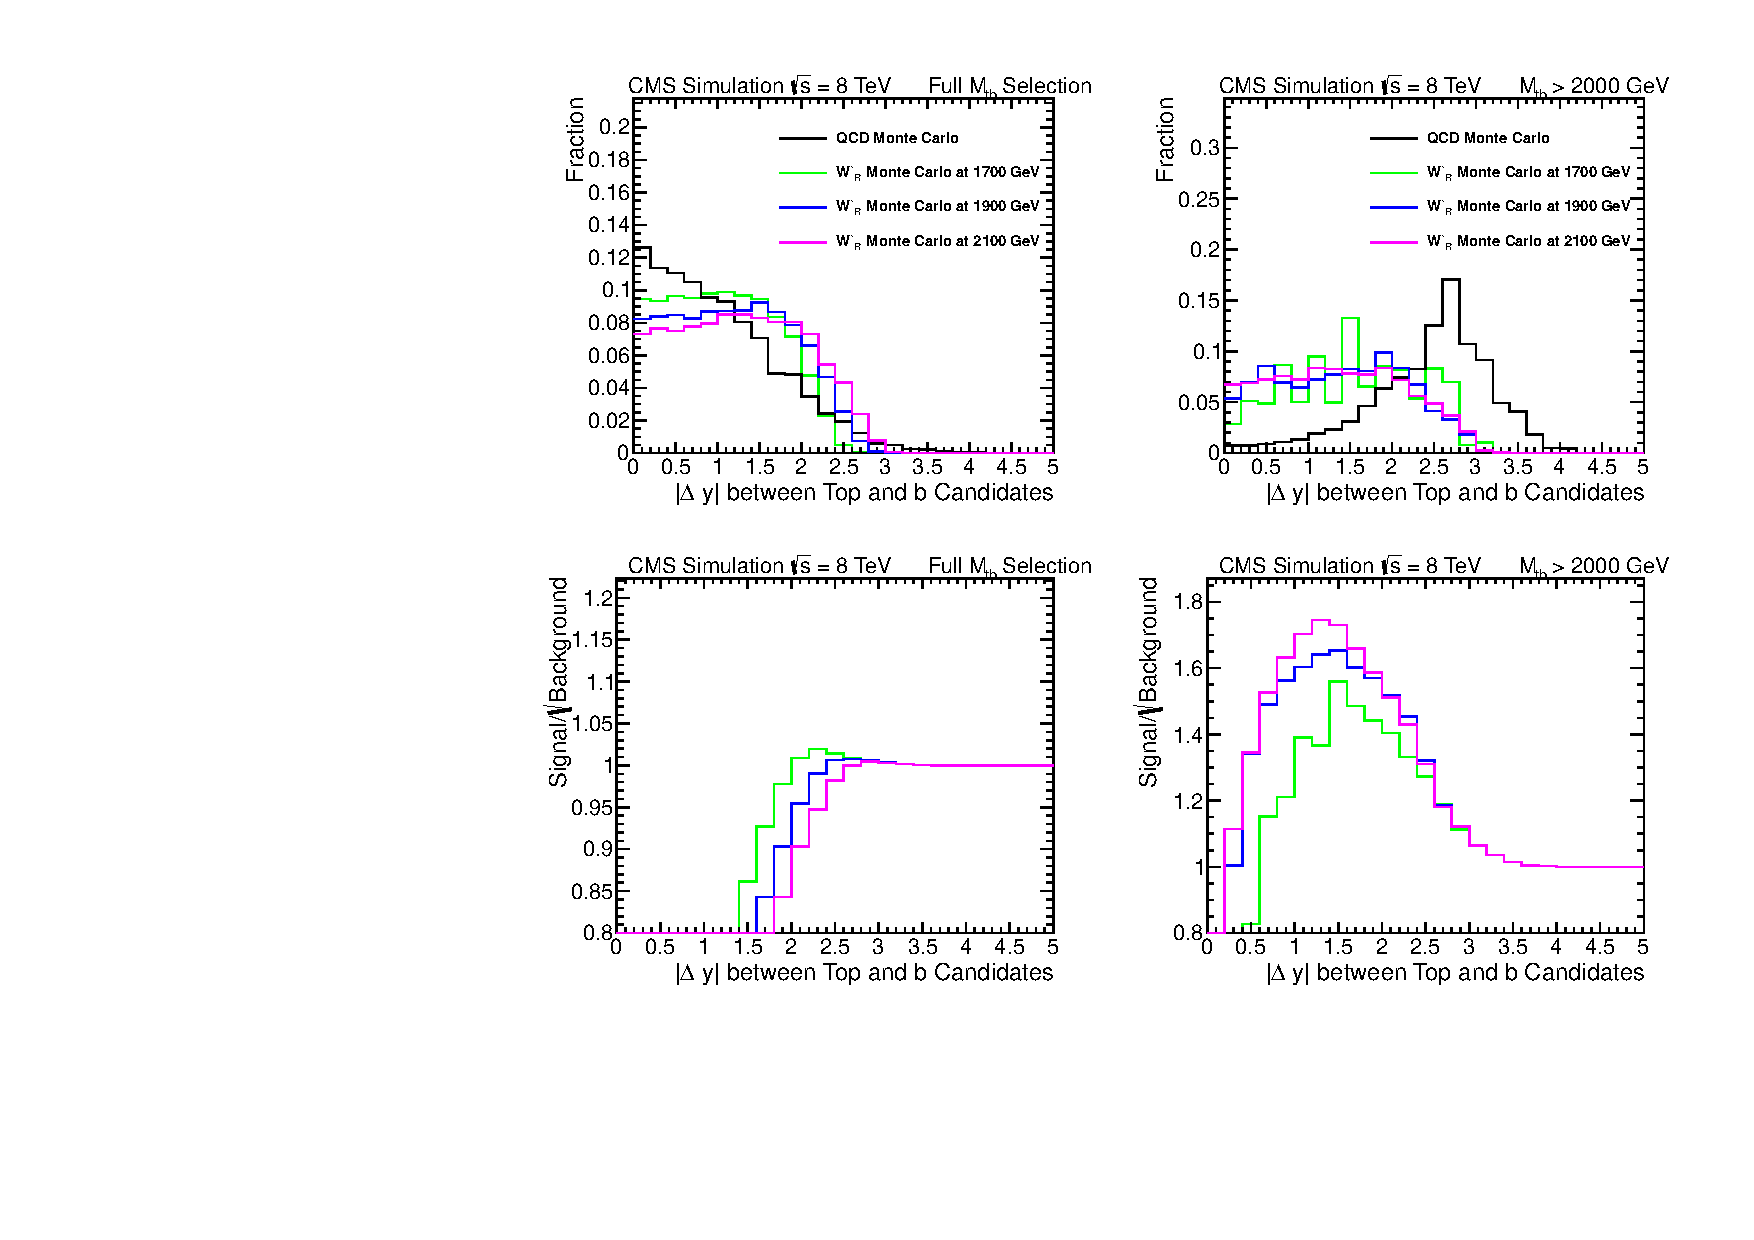
\includegraphics[width=1.0\textwidth]{AN-13-004/figs/drapCompqcdandsignal}
\caption{Comparison of $|\Delta y|$ in signal and QCD Monte Carlo for the full selection and only events with $M_{\tbbar} > 2000~\GeV$}
\label{figs:CutComp}
\end{figure}



\section{b-jet Identification}
\label{sec:btagging}
To enhance the sensitivity of the analysis, the Combined Secondary Vertex (CSV) b-tagging algorithm is applied to the subleading jet. We use the standard operating point CSVM (CSV $>$ 0.679).
%after optimizing S/$\sqrt{B}$ using all 8TeV supported b-tagging algorithms and operating points.  
Due to the fact that our signal content 
contains only $\tbbar$ and the only Monte Carlo used in background estimation is $\ttbar$, the Monte Carlo to data scale factor used in the analysis for b-tagging 
is the b-tagging Scale Factor for b quarks ($SF_b$).  We use the suggested scale factor parameterized in $\pt$ with the following functional form for 
b candidate jet $\pt < 800~\GeV$

\begin{eqnarray}
SF_b = 0.938887 + 0.00017124\times \pt - 2.76366 \times 10^{-07} \times \pt^2 
\end{eqnarray}
Any b candidate jet with $\pt > 800~\GeV$ is weighted with $SF_b$ evaluated at 800$~\GeV$.  The parameterized $SF_b$ is the 
suggested EPS13 prescription \cite{CMS-PAS-BTV-13-001} from the b-tagging POG generated from measurements in both muon-jet and ttbar data representing 20$~\fbinv$ of integrated 
luminosity. The uncertainty associated with this scale factor parameterization is described in Chapter \ref{sec:systematics}.  b-tagging operating points 
and scale factors have been validated for use with anti-kt jets with a R value of 0.5 (AK5 jets).  In our kinematic regime it is assumed that the change in cone size 
will have a small effect. We apply an additional $2\%$ systematic uncertainty to the signal Monte Carlo samples used in the analysis. This is a conservative estimate of the uncertainty, validated by the following study: 

For the $2700~\GeV$ signal sample, we 
included both AK5 and CA8 jets in the event selection.  All jets considered were required to be in our pt range ($\pt > 350~\GeV$).  We attempt to match a CA8 jet to 
the corresponding AK5 jet using a constraint on $\eta$ and $\phi$ ($\Delta$R $< 0.3$ ).  The results were 579041 CA8 jets pass pt cut,
of these, 567155 pass the $\eta$ , $\phi$ matching to AK5 jets.  Of the matched jets, $96.9\%$ record the same value for the CSVM cut (pass or fail). In addition, 
the ratio of b-tagging efficiencies for both AK5 and CA8 were found to be within a $2\%$ deviation (see Figure \ref{figs:btageff}).  To rule out a bias based on the 
known differences in pt for CA8 and AK5 jets, the efficiencies and uncertainties were extracted from plots using only the pt of the CA8 jet.  
The fit on the b-tagging efficiency ratio for CA8 and AK5 jets can be interpreted as an upper bound on the uncertainty due to this effect.
We also checked this process for $1300~\GeV$ and $1900~\GeV$ signal samples and found results consistent with this $2\%$ error. 
We have verified this systematic uncertainty with the BTV group, and it is approved for use in our analysis.

\begin{figure}[htcb]
\centering
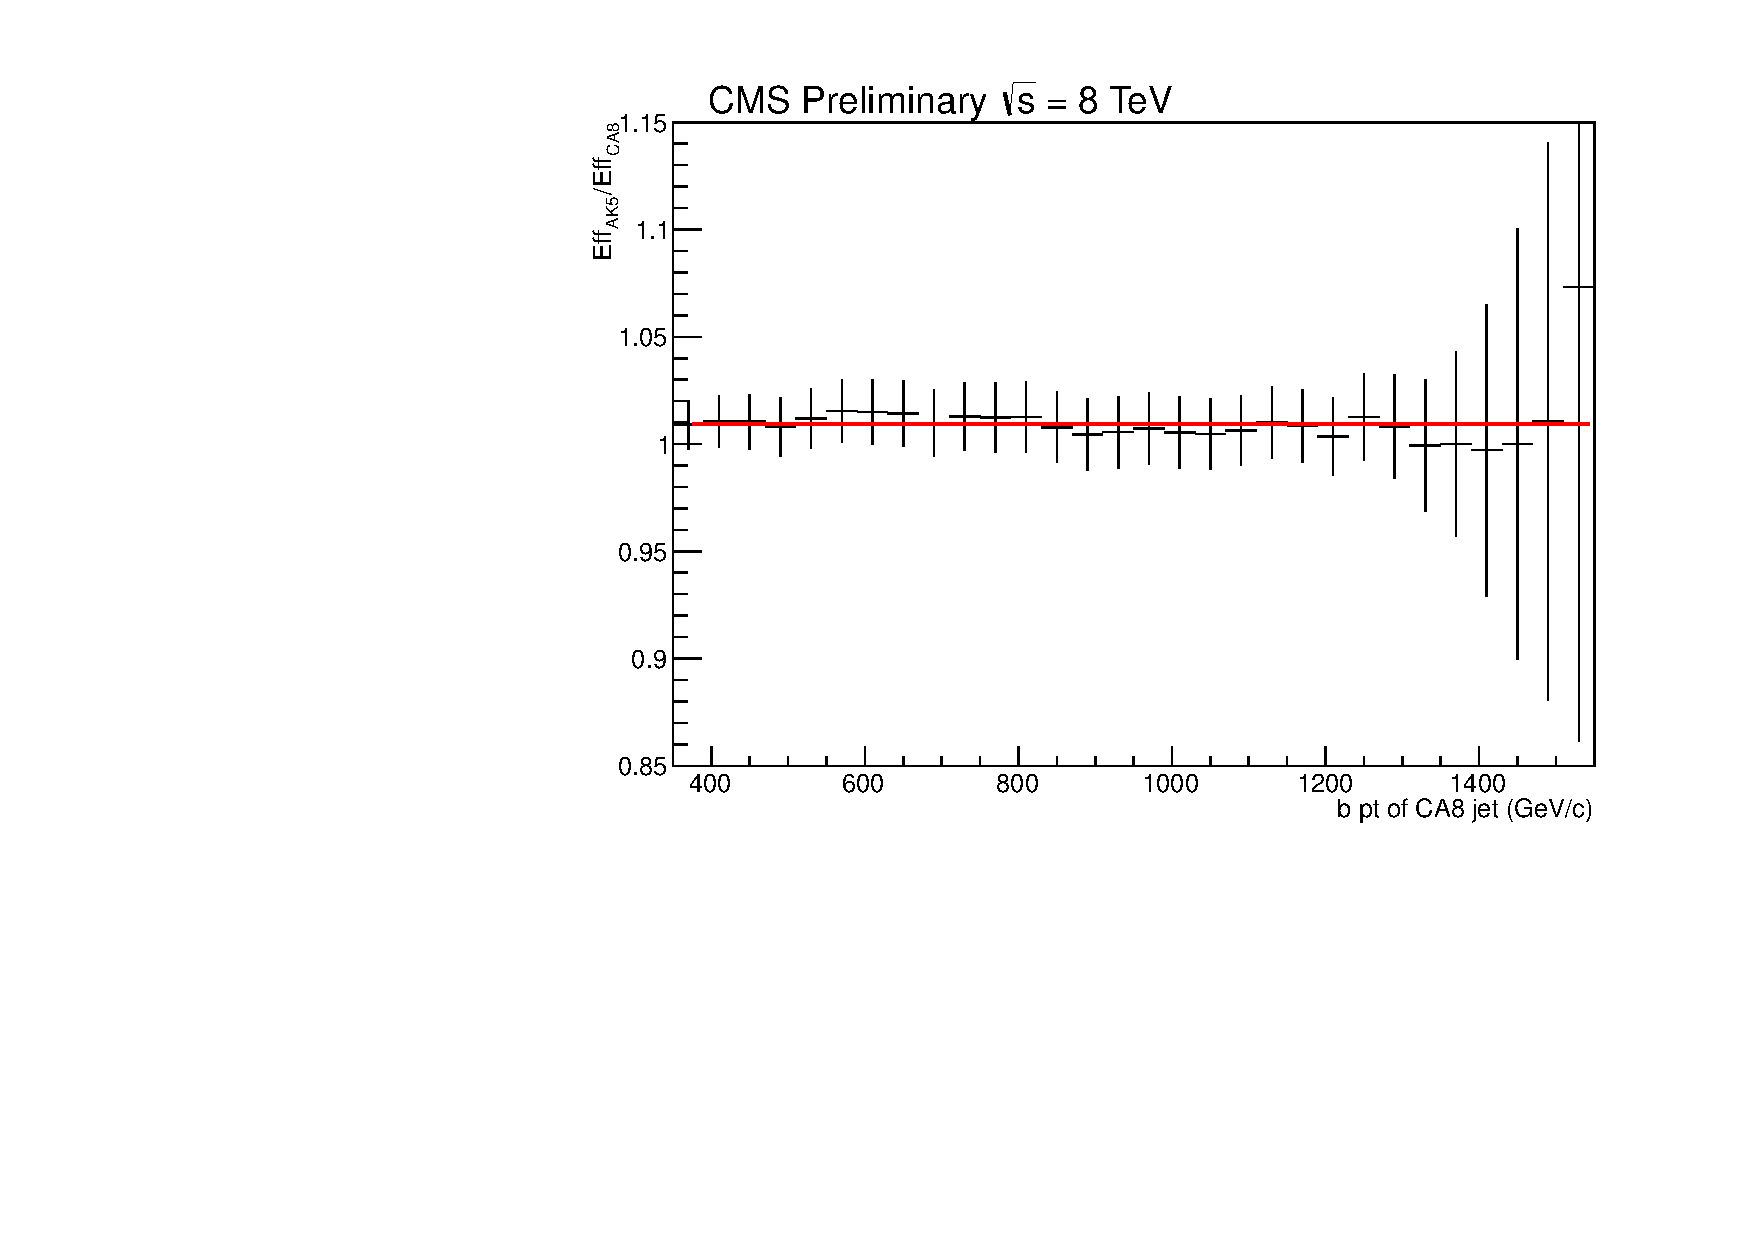
\includegraphics[width=0.9\textwidth]{AN-13-004/figs/EfficiencyCompCAptr32700.pdf}
\caption{Ratio of the AK5 b-tagging rate to the CA8 b-tagging rate. Fitting this to a constant gives us a value of 1.0098 $\pm$ 0.0031.  This can 
be considered an upper limit on the uncertainty for the change in $SF_b$ for CA8 jets}

\label{figs:btageff}
\end{figure}

After the full top tagging selection is complete, there is a substantial fraction of $\ttbar$ in the full selection.
Additionally, there is a large uncertainty in the $\ttbar$ Monte Carlo contribution, so discriminating signal from $\ttbar$ becomes important.  
In $\wpr$ signal Monte Carlo, the sub-leading b candidate jet is usually a true b jet, but in $\ttbar$ this jet is commonly a merged W or top jet. 
To this effect, the b candidate jet is required to have a mass $M_b < 70~\GeV$ in the full selection.  The value for this cut is set near the peak of the Signal/$\sqrt{\text{Background}}$ distribution (see Figure \ref{figs:BmassCOMP}).


\begin{figure}[htcb]
\begin{center}
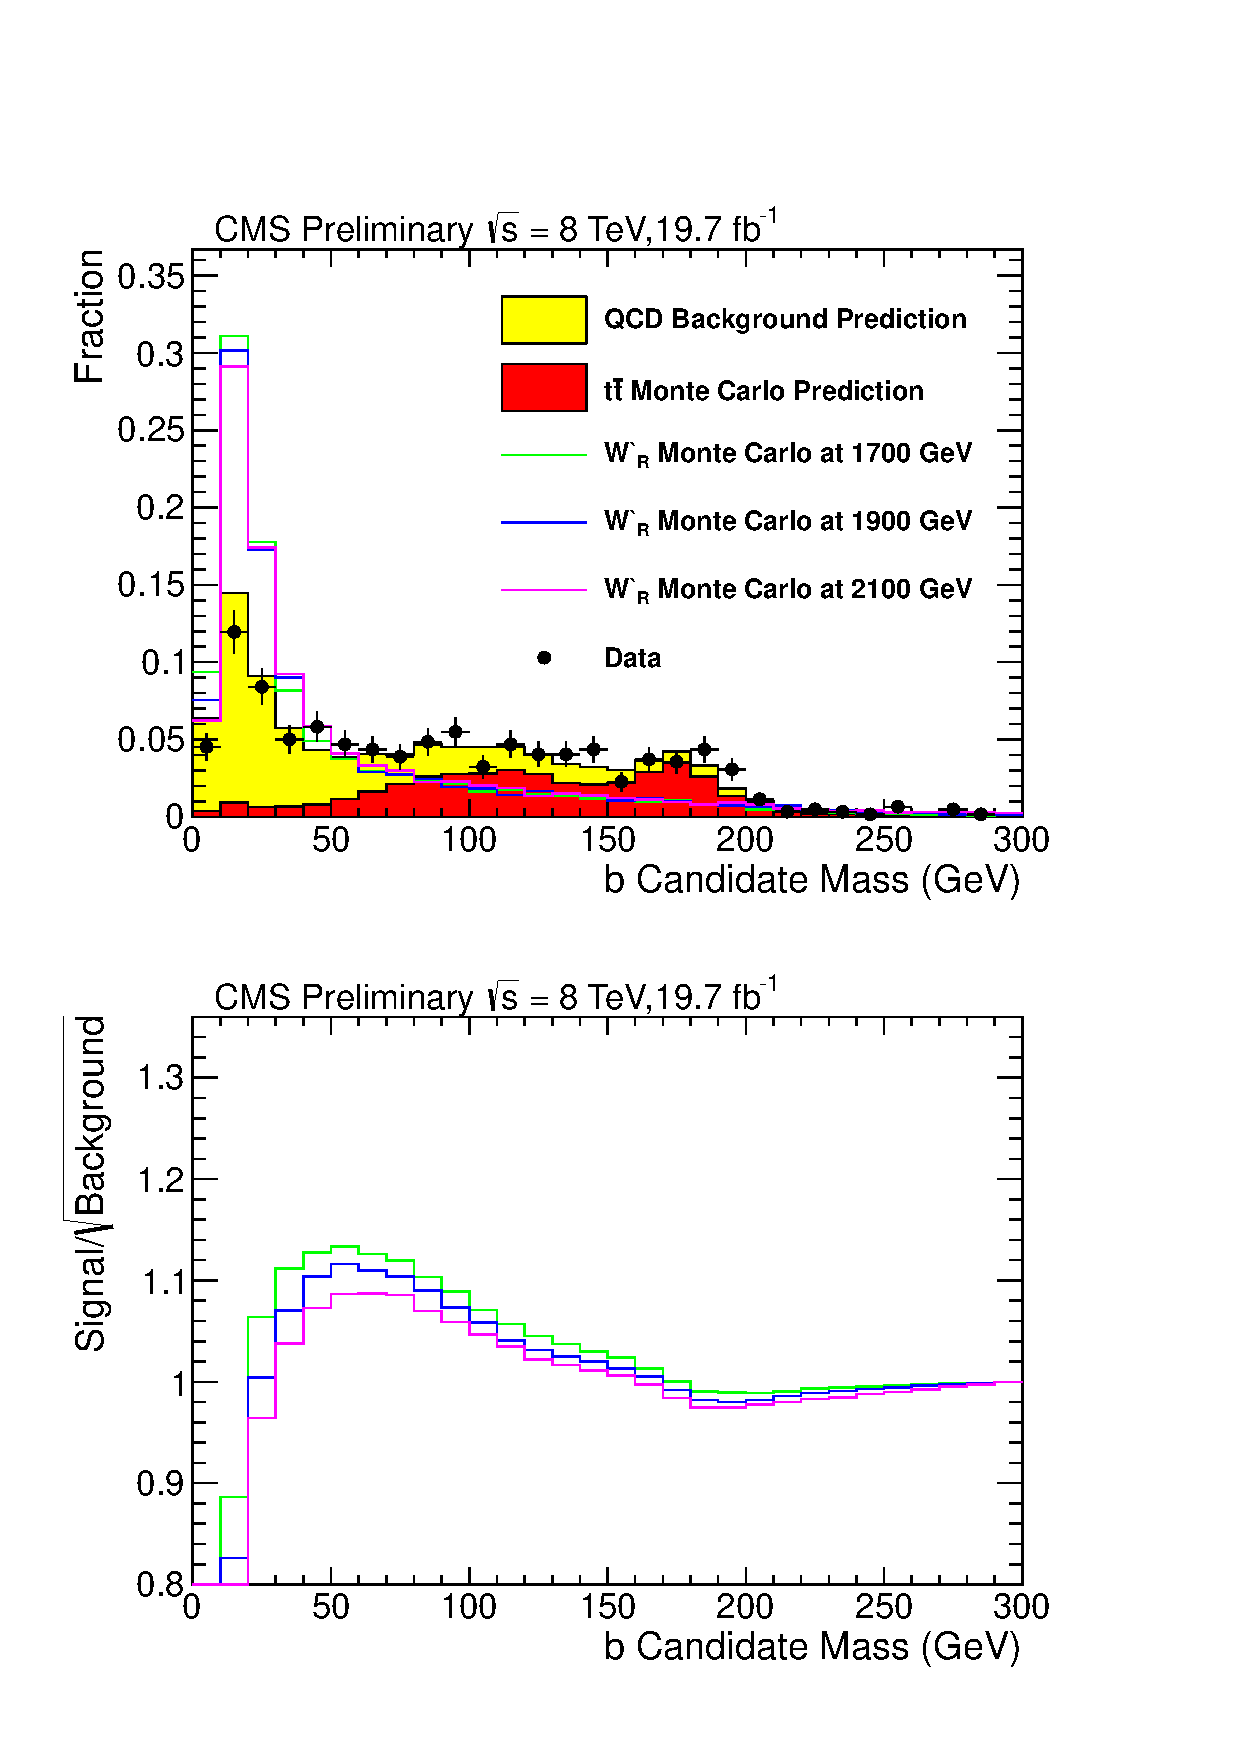
\includegraphics[width=0.7\textwidth]{AN-13-004/figs/bmassdatatosigwithdata.pdf}
\caption{
b candidate mass distributions in data, background, and signal.  Plot of Signal/$\sqrt{\text{Background}}$ (bottom), derived from the top plot. 
This plot includes the full top tagging selection using the background estimation procedure outlined in Chapter \ref{sec:backgroundEstimation}.
}
\label{figs:BmassCOMP}
\end{center}
\end{figure}


\section{Reconstruction of W' Invariant Mass}
\label{sec:fullselection}
The full selection for the reconstruction of the $\wpr$ invariant mass then includes the following offline cuts.
\begin{itemize}
\item One jet with $\pt > 450~\GeV$ identified with the CMS top tagging algorithm as well as subjet b-tagging and N-subjettiness discrimination.
\item One jet with $\pt > 370~\GeV$ with a CSVM b tag and mass$ < 70~\GeV$
\item $|\Delta \phi| > \pi/2$ between the two jets
\item $|\Delta y|$ between the two jets $<$ 1.6 
\end{itemize}
The cutflow for this selection in data, $\ttbar$ Monte Carlo, and right-handed $\wpr$ signal Monte Carlo can be found in Table \ref{table:Cutflow}.
Figure \ref{figs:GCFS} shows this full selection in signal Monte Carlo for various $\wpr$ masses.  



\begin{sidewaystable}
\begin{center}
\begin{small}

\scalebox{0.7}{
\begin{tabular}{c||cccccccccc}
\multicolumn{7}{c}{Number of Selected Events} \\
\hline\hline
\bf{Sample} & \bf{$2 jets$} & \bf{$\pt$} & \bf{$|\Delta y|$} & \bf{$M_{top}$} & \bf{$Nsubjets$} &  \bf{$Minmass$}  & $SJ_{\text{CSVMAX}}$  & $\tau_3/\tau_2$ & $M_{b}$ & \bf{$CSV$}\\
\hline
Data & 13854873$\pm$3722 & 4305244$\pm$2075 & 3376771$\pm$1838 & 992949$\pm$996 & 557489$\pm$747 & 318520$\pm$564 & 50642$\pm$225 & 7200$\pm$85 & 4463$\pm$67 & 277$\pm$17\\
QCD & --- & --- & --- & --- & --- & --- & --- & --- & --- & 248$\pm$4\\
ttbar & 12185$\pm$27.3 & 4718$\pm$17.9 & 4220$\pm$16.9 & 3217$\pm$14.4 & 2742$\pm$13.3 & 2508$\pm$12.6 & 1689$\pm$10.0 & 1024$\pm$7.8 & 178$\pm$3.6 & 37$\pm$1.4\\
M($W`_{R}$) = 1900 & 806$\pm$1.4 & 739$\pm$1.3 & 553$\pm$1.2 & 429$\pm$1.0 & 340$\pm$0.9 & 304$\pm$0.9 & 170$\pm$0.6 & 88$\pm$0.4 & 68$\pm$0.4 & 16$\pm$0.2\\
M($W`_{R}$) = 2100 & 401$\pm$0.7 & 372$\pm$0.7 & 268$\pm$0.6 & 209$\pm$0.5 & 163$\pm$0.4 & 143$\pm$0.4 & 76$\pm$0.3 & 38$\pm$0.2 & 29$\pm$0.2 & 6$\pm$0.1\\
M($W`_{L}$) = 1900 & 796$\pm$2.4 & 703$\pm$2.3 & 531$\pm$2.0 & 414$\pm$1.8 & 312$\pm$1.6 & 274$\pm$1.5 & 138$\pm$1.0 & 58$\pm$0.6 & 44$\pm$0.6 & 10$\pm$0.3\\
M($W`_{L}$) = 2100 & 430$\pm$1.6 & 364$\pm$1.5 & 268$\pm$1.3 & 205$\pm$1.1 & 152$\pm$1.0 & 130$\pm$0.9 & 63$\pm$0.6 & 27$\pm$0.4 & 20$\pm$0.3 & 4$\pm$0.2\\
\end{tabular}
}
\caption{The number of selected events after successive selections as scaled to an integrated luminosity of 19.7~$\fbinv$.  Table reads left to right where the current column implies the previous selection.  The quoted uncertainty is statistical only.  QCD background expectation is only recorded for the full selection, as the average b-tagging rate takes into account the QCD background b fraction increase from b-tagging and subjet b-tagging.  
The first column additionally represents the hemispherical $\delta \phi$ selection between the leading jets.  
The column labeled $\pt$ represents the $\pt$ selection placed on both leading jets.  The signal events are normalized to theory cross-section.}
\label{table:Cutflow}
\end{small}
\end{center}
\end{sidewaystable}




%\begin{sidewaystable}
%\begin{center}
%\begin{small}
%\begin{tabular}{cccccccccc}
%\multicolumn{7}{c}{Data Cutflow} \\
%\hline\hline
%\bf{2 jets} & \bf{$\pt$} & \bf{$|\Delta y|$} & \bf{$M_{top}$} & \bf{$Nsubjets$} &  \bf{$Minmass$} & \bf{$CSV$}  & $\tau_3/\tau_2$ & $M_{b}$ & $SJ_{\text{CSVMAX}}$\\
%\hline
%71.10\% & 22.04\% & 17.28\% & 5.08\% & 2.85\% & 1.63\% & 0.09\% & 0.01\% & 0.007\% & 0.001\%\\
%\end{tabular}
%\caption{Cutflow for Data. Table reads left to right where the current column implies the previous cuts}
%\vspace{1cm}

%\begin{tabular}{cccccccccc}
%\multicolumn{7}{c}{$\ttbar$ Cutflow} \\
%\hline\hline
%\bf{2 jets} & \bf{$\pt$} & \bf{$|\Delta y|$} & \bf{$M_{top}$} & \bf{$Nsubjets$} &  \bf{$Minmass$} & \bf{$CSV$}  & $\tau_3/\tau_2$ & $M_{b}$ & $SJ_{\text{CSVMAX}}$\\
%\bf{2 jets $\pt > 150$} & \bf{Jet1 $\pt > 450$ ; Jet2 $\pt > 370$} & %\bf{$|\Delta y| < 1.6$} & \bf{$140 < M_{top} < 250$} & \bf{$Nsubjets > 2$} &  %\bf{$Minmass > 50$} & \bf{$CSV > 0.679$} & $\tau_3/\tau_2 <0.55$ & $Jet2 Mass < 70$ & $SJ_{\text{CSVMAX}} > 0.679$  \\
%\hline
%26.50\% & 0.91\% & 0.82\% & 0.62\% & 0.52\% & 0.47\% & 0.12\% & 0.06\% & 0.009\% & 0.007\%\\
%\end{tabular}
%\caption{Cutflow for TTbar Monte Carlo. Table reads left to right where the current column implies the previous cuts}
%\vspace{1cm}

%\begin{tabular}{c|cccccccccc}
%\multicolumn{8}{c}{Signal Cutflow} \\
%\hline\hline
%\bf{$M_{\wpr}$} & \bf{2 jets $\pt > 150$} & \bf{Jet1 $\pt > 450$ ; Jet2 $\pt > 370$} & \bf{$|\Delta y| < 1.6$} & \bf{$140 < M_{top} < 250$} & \bf{$Nsubjets > 2$} &  \bf{$Minmass > 50$} & \bf{$CSV > 0.679$} & $\tau_3/\tau_2 <0.55$ & $Jet2 Mass < 70$ & $SJ_{\text{CSVMAX}} > 0.679$ \\
%\bf{$M_{\wpr}$} & \bf{2 jets} & \bf{$\pt$} & \bf{$|\Delta y|$} & \bf{$M_{top}$} & \bf{$Nsubjets$} &  \bf{$Minmass$} & \bf{$CSV$}  & $\tau_3/\tau_2$ & $M_{b}$ & $SJ_{\text{CSVMAX}}$\\
%\hline
%1300 & 77.86\% & 44.33\% & 42.09\% & 27.24\% & 22.55\% & 20.31\% & 7.19\%& 3.79\%& 3.08\%& 2.16\%\\
%1500 & 78.25\% & 52.64\% & 45.20\% & 32.66\% & 26.69\% & 24.15\% & 7.42\%& 3.74\%& 2.95\%& 2.02\%\\
%1700 & 78.01\% & 57.37\% & 45.44\% & 34.47\% & 27.59\% & 24.92\% & 6.67\%& 3.22\%& 2.49\%& 1.68\%\\
%1900 & 77.20\% & 59.36\% & 44.40\% & 34.51\% & 27.19\% & 24.26\% & 5.74\%& 2.72\%& 2.06\%& 1.34\%\\
%2100 & 76.04\% & 59.72\% & 42.95\% & 33.56\% & 26.05\% & 22.70\% & 4.87\%& 2.20\%& 1.63\%& 1.02\%\\
%2300 & 74.20\% & 58.37\% & 40.87\% & 31.80\% & 24.63\% & 20.70\% & 4.14\%& 1.87\%& 1.37\%& 0.84\%\\
%2700 & 69.36\% & 51.81\% & 35.51\% & 27.13\% & 21.51\% & 16.32\% & 3.06\%& 1.34\%& 0.99\%& 0.61\%\\
%3100 & 63.12\% & 40.89\% & 28.57\% & 21.23\% & 17.34\% & 12.28\% & 2.54\%& 1.15\%& 0.86\%& 0.55\%\\
%\end{tabular}
%\caption{Cutflow for Right-Handed $\wpr$ signal Monte Carlo. Table reads left to right where the current column implies the previous cuts}
%\label{table:Cutflows}
%\end{small}
%\end{center}
%\end{sidewaystable}

\begin{figure}[htcb]
\begin{center}
\subfigure{\label{figs:GCFSright}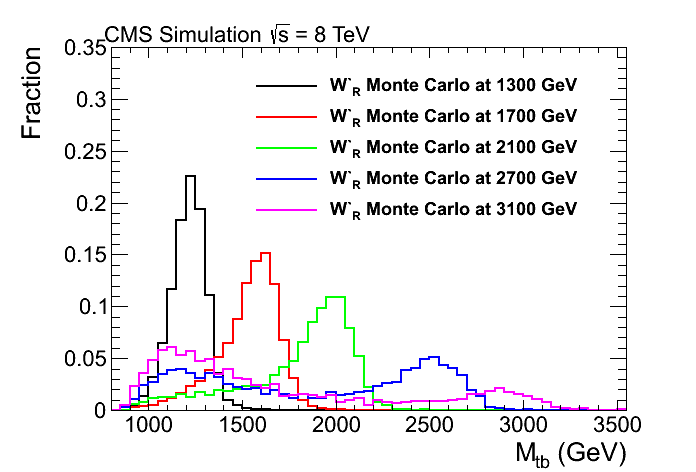
\includegraphics[width=0.45\textwidth]{AN-13-004/figs/SignalMCFScomparison}}\\
\subfigure{\label{figs:GCFSleft}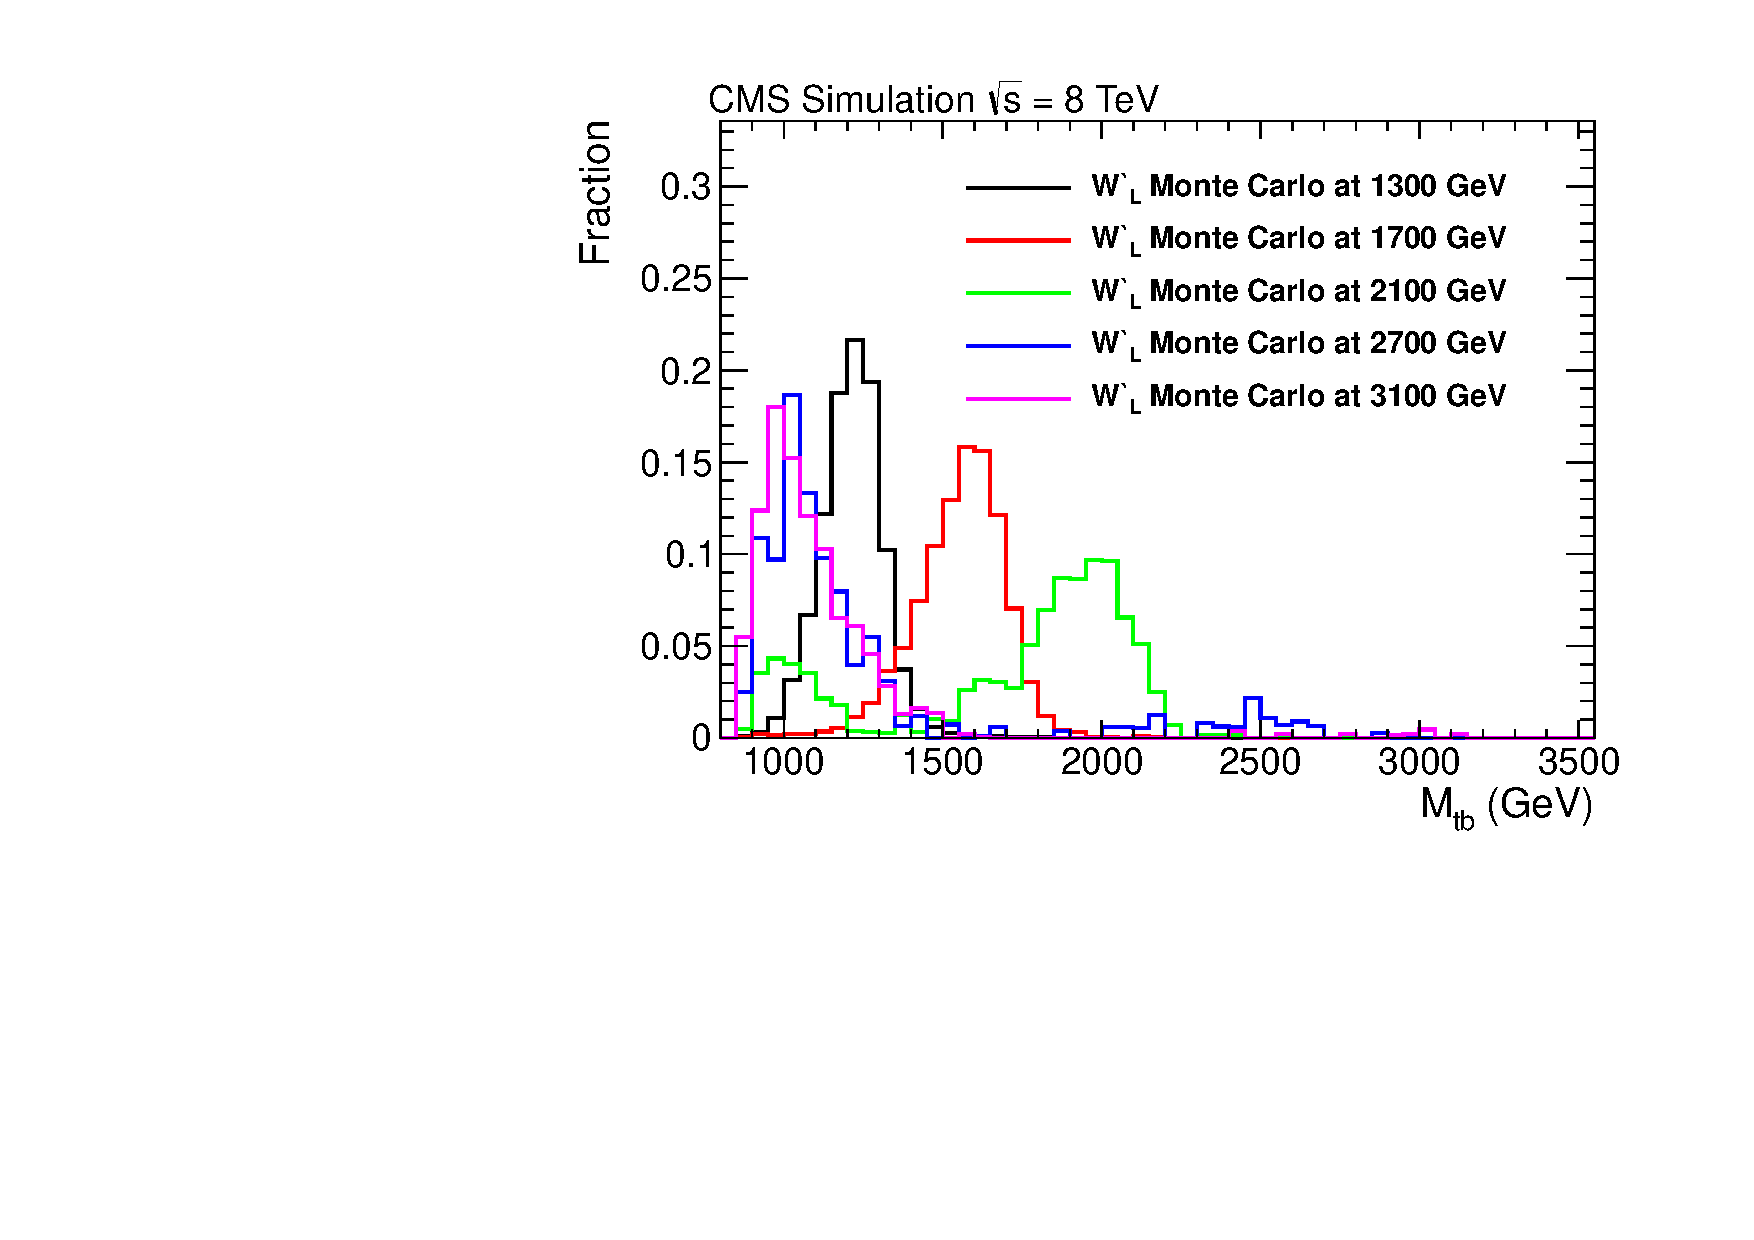
\includegraphics[width=0.45\textwidth]{AN-13-004/figs/SignalLeftMCFScomparison.pdf}}
\subfigure{\label{figs:GCFSmixed}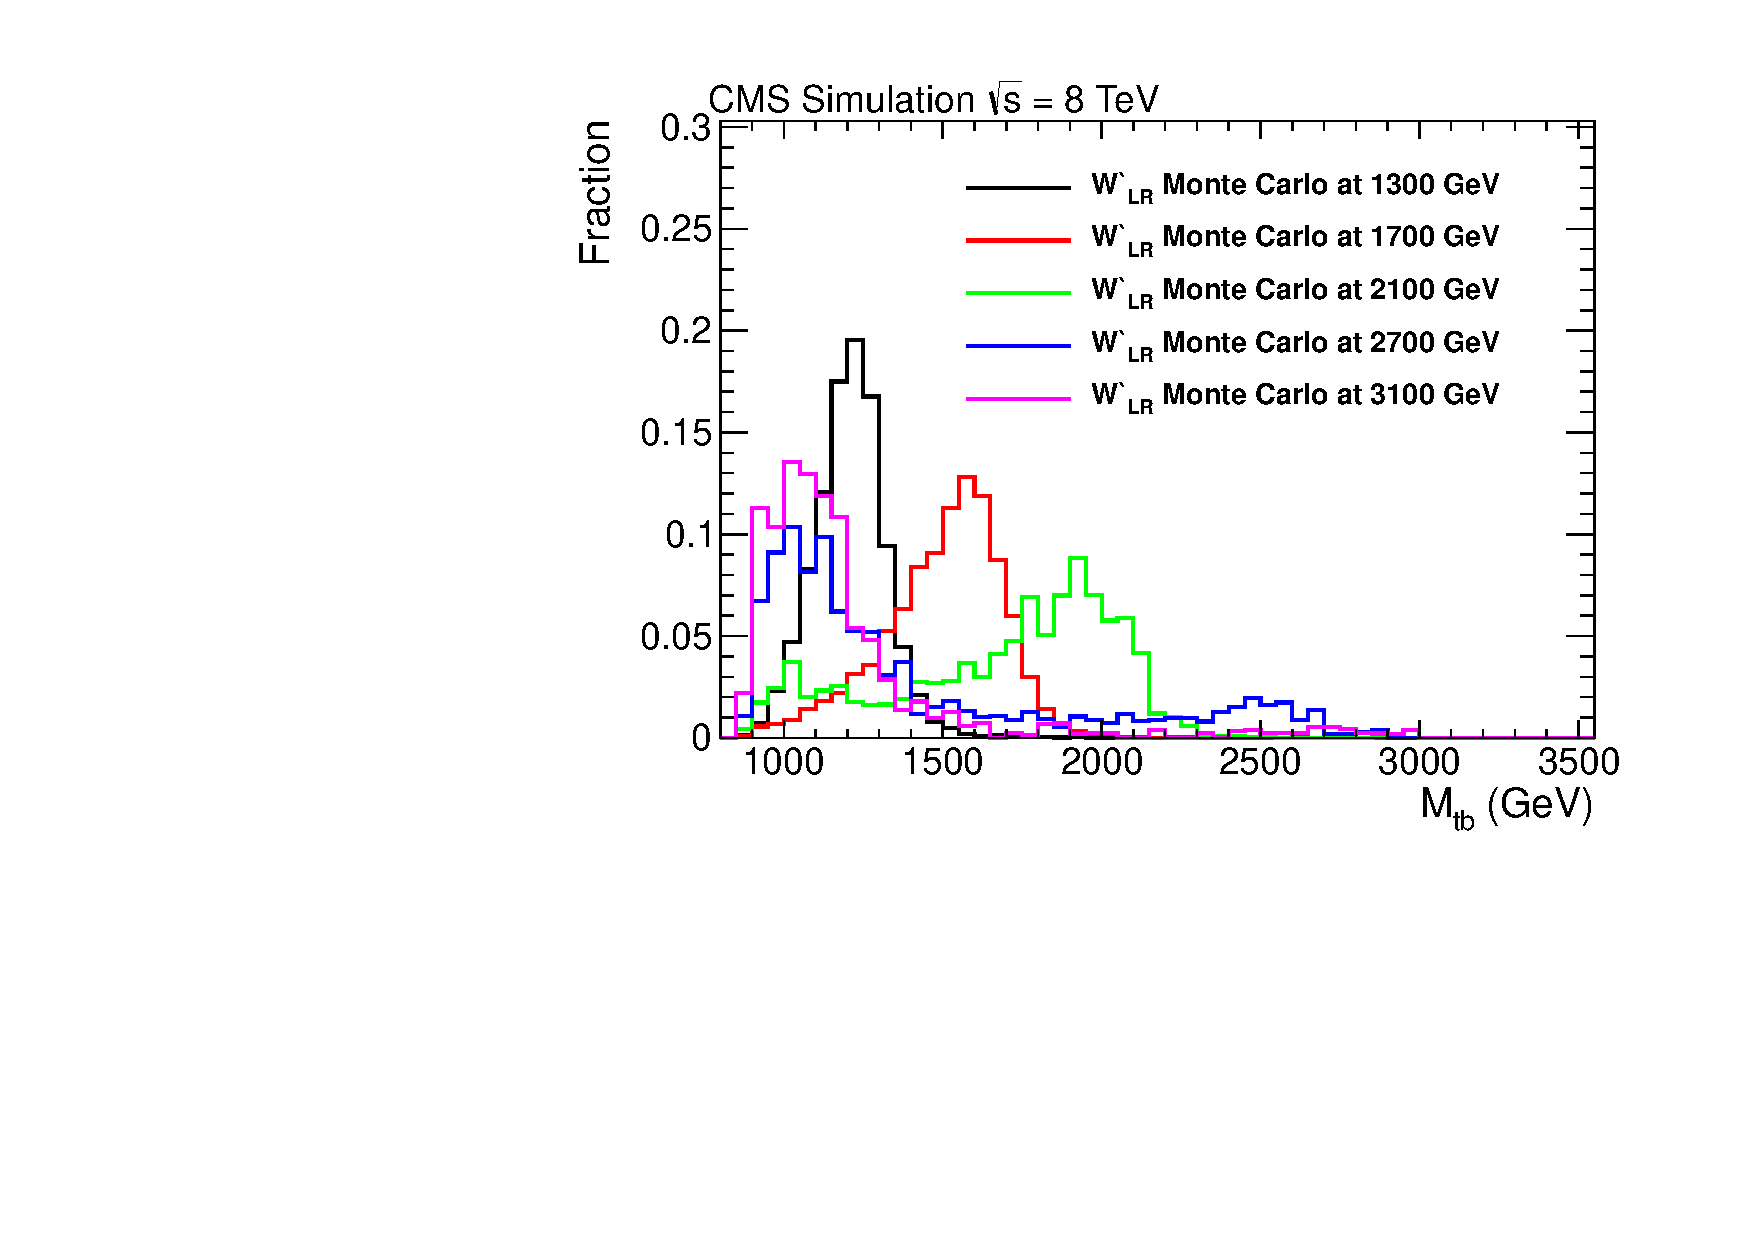
\includegraphics[width=0.45\textwidth]{AN-13-004/figs/SignalMixedMCFScomparison.pdf}}
\caption{
Full selection applied to $W`_{R}$ (top) $W`_{L}$ (bottom-left) and $W`_{LR}$ (bottom-right).  The bimodal structure seen in the $M_{tb}$ spectrum for high $\wpr$ mass is a feature common to high-mass large-width resonances and represents the superposition of a $\wpr$ resonance and a rapidly falling parton distribution function. 
}
\label{figs:GCFS}
\end{center}
\end{figure}

%\begin{figure}[htcb]
%\centering
%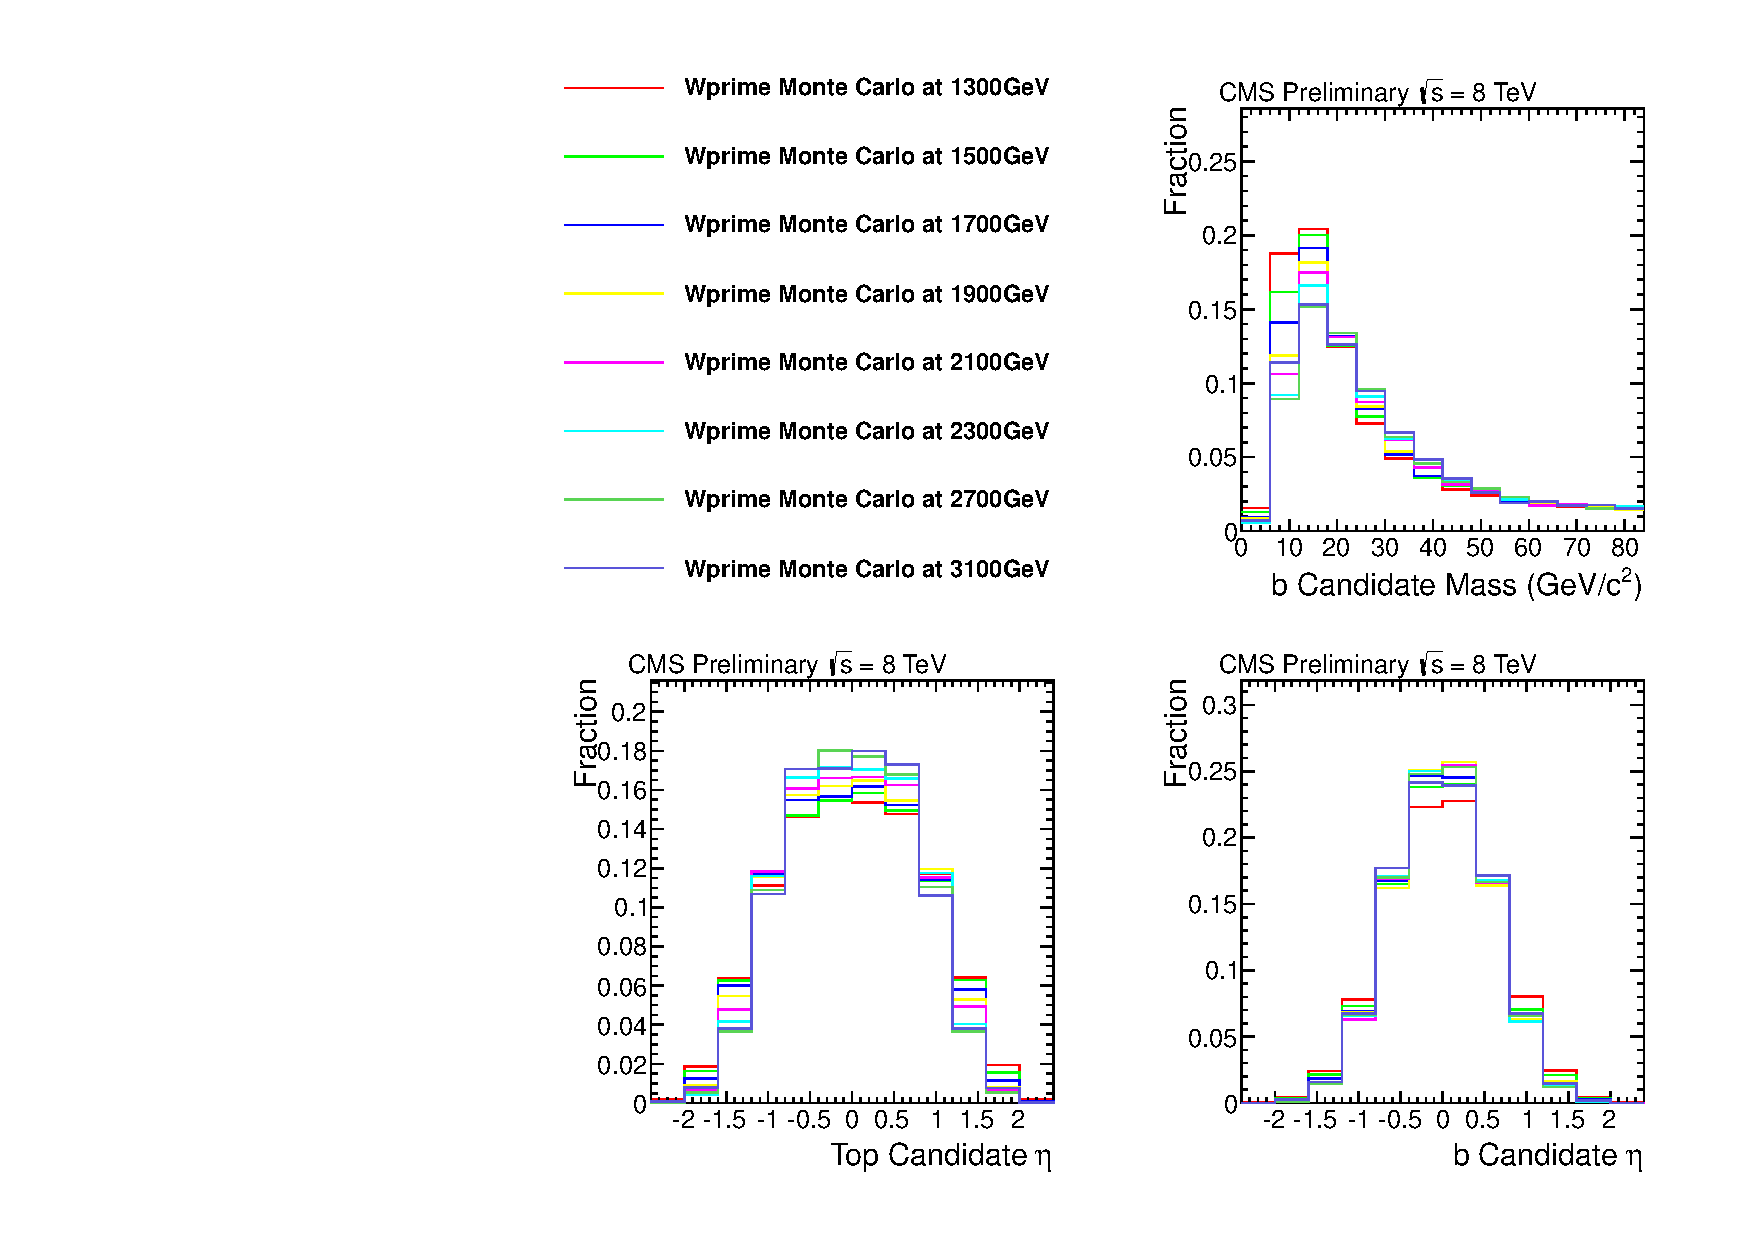
\includegraphics[width=0.9\textwidth]{AN-13-004/figs/KinPlots_Signal1}
%\caption{Full selection in right-handed $\wpr$ signal Monte Carlo kinematic distributions}
%\label{figs:kinplotssignal1}
%\end{figure}

%\begin{figure}[htcb]
%\centering
%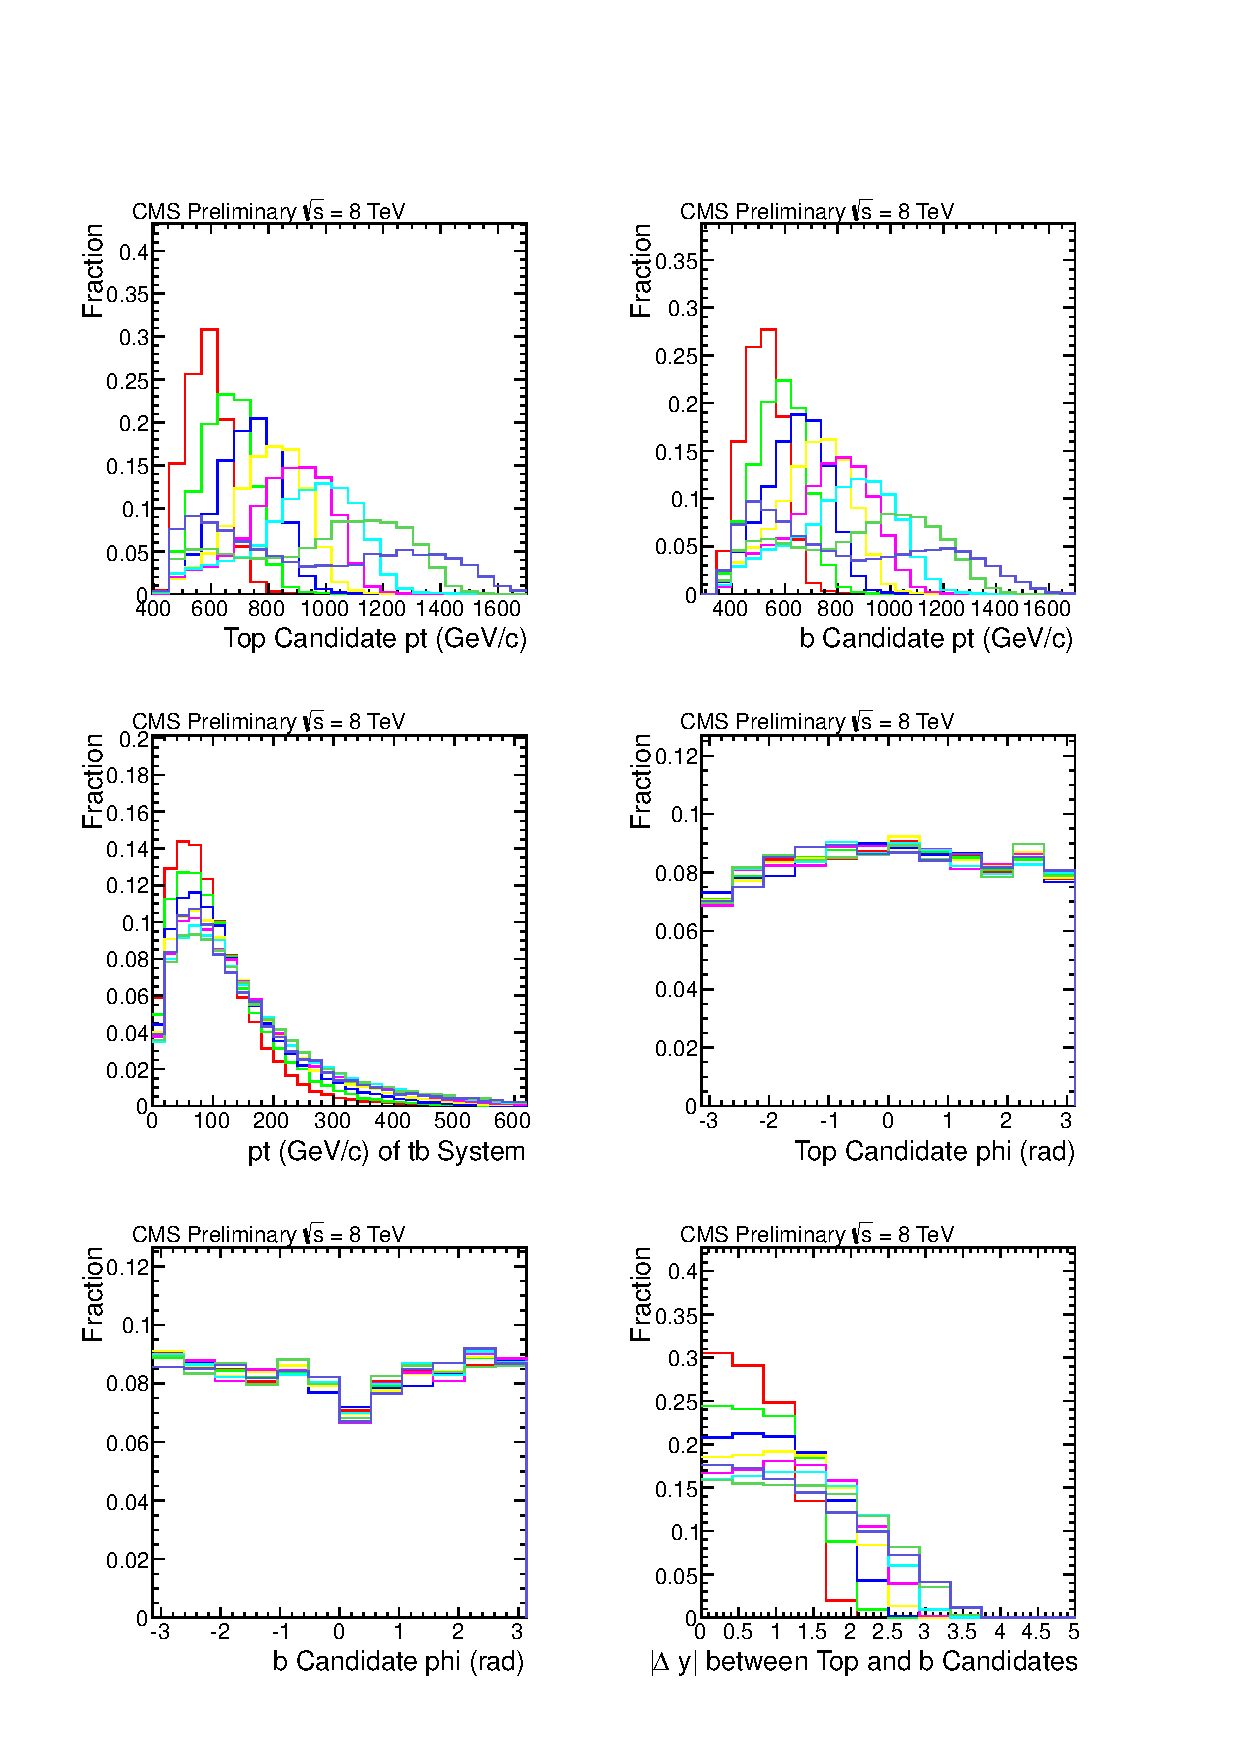
\includegraphics[width=0.9\textwidth]{AN-13-004/figs/KinPlots_Signal2}
%\caption{Full selection in right-handed $\wpr$ signal Monte Carlo kinematic distributions}
%\label{figs:kinplotssignal2}
%\end{figure}
\clearpage

% \section{Validation of Substructure in semi-leptonic Data}
\label{sec:semilep}
Use of the top tagging algorithm described in section ~\ref{sec:toptagging} requires an understanding of how jet substructure affects kinematics in the signal region.
We use the same prescription for extracting the subjet selection efficiency and subjet energy scale as Z` $\to \ttbar$ all hadronic described in reference  \cite{7tevZprime}.

To measure the relevant substructure variables, we use single muon datasets given in table ~\ref{table:singlemusets} 

\begin{table}
\begin{center}
\bf{Single Muon Datasets}
\begin{tabular}{|p{0.7\linewidth}|p{0.3\linewidth}|}
\hline
\bf{Dataset} & \bf{Luminosity ($\pbinv$)} \\
\hline
/SingleMu/Run2012A-13Jul2012-v1/AOD & 804 \\
/SingleMu/Run2012B-13Jul2012-v1/AOD & 4429 \\
/SingleMu/Run2012C-PromptReco-v1/AOD 	 & 495 \\
/SingleMu/Run2012C-PromptReco-v2/AOD 	 & 5469 \\
/SingleMu/Run2012D-PromptReco-v1/AOD 	 & 4183 \\
\hline
Total Analyzed Luminosity &  15380 \\
\hline
\end{tabular}
\bf{Monte Carlo Datasets} \\
\begin{tabular}{|p{0.7\linewidth}|p{0.3\linewidth}|}
\hline
\bf{Dataset} & \bf{Cross section(pb)} \\
\hline
/TTJets\_MassiveBinDECAY\_TuneZ2star\_8TeV-madgraph-tauola/Summer12\_DR53X-PU\_S10\_START53\_V7A-v1/AODSIM & 225.0\\
/WJetsToLNu\_TuneZ2Star\_8TeV-madgraph-tarball/Summer12\_DR53X-PU\_S10\_START53\_V7A-v2/AODSIM & 37509.0\\
/T\_t-channel\_TuneZ2star\_8TeV-powheg-tauola/AODSIM & 56.4\\
/Tbar\_t-channel\_TuneZ2star\_8TeV-powheg-tauola/AODSIM & 30.7\\
/Tbar\_tW-channel-DR\_TuneZ2star\_8TeV-powheg-tauola/AODSIM & 11.1\\
/T\_tW-channel-DR\_TuneZ2star\_8TeV-powheg-tauola/AODSIM & 11.1\\
/T\_s-channel\_TuneZ2star\_8TeV-powheg-tauola/AODSIM & 3.79\\
/Tbar\_s-channel\_TuneZ2star\_8TeV-powheg-tauola/AODSIM & 1.76\\
/DYJetsToLL\_M-50\_TuneZ2Star\_8TeV-madgraph-tarball/Summer12\_DR53X-PU\_S10\_START53\_V7A-v1/AODSIM & 3503.71\\
\hline
\end{tabular}
\end{center}
\caption{Single Muon datasets and Monte Carlo samples used in the analysis.  These samples are used to extract variables related to jet substructure.}
\label{table:singlemusets}
\end{table}

The following selection is designed to increase the purity of $\ttbar$ events and is applied to the signal region.  We define the following cuts. 
\begin{itemize}
\item Tight Muon Selection
\begin{itemize}
\item $p_T > 45$ GeV/$c$
\item $|\eta| < 2.1$
\item The muon is from the highest Pt primary vertex
\item \verb!isTracker()! and \verb!isGlobalMuon()!
\item $\chi^2 / N_{DOF} < 10$
\item $N_{Tracker Hits} > 10$
\item $N_{Pixel Hits} > 0$
\item $N_{Muon Hits} > 0$
\item $d_0 < 0.02$ cm (with respect to the hardest DAF PV)
\item $I_{rel} < 0.12$ (using a cone size of $R=0.4$, and using $\Delta\beta$ corrections)
\item Number of matched stations $> 0$
\item no other isolated muons are allowed
\end{itemize}
\end{itemize}

The following selection is designed to simulate backgrounds in the analysis that are not simulated by 
w+jets or $\ttbar$ Monte Carlo  events and defines the sideband for the single muon analysis.  We define the following cuts.
\begin{itemize} 
\item Loose Muon Selection
\begin{itemize}
\item Can be a tracker muon OR a global muon
\item $p_T > 45$ GeV/$c$
\item Not contained in a sub-leading primary vertex
\item $I_{rel} < 0.20$
\end{itemize}
\end{itemize}

In the hemisphere opposite the isolated muon, we study the case of a dijet top, where the b and W candidate jets are both resolved.  
The following selection is required on the jets in this hemisphere for extraction of the top mass. 

\begin{itemize}
\item Hadronic Hemisphere Selection
\begin{itemize}
\item Two jets with  $p_T > 30$ $\GeVc$
\item Leading jet is required to have $p_T > 200$ $\GeVc$
\item Mass drop variable $\mu = \frac{m_1}{m_\text{jet}}$.  We require a mass drop $\mu < 0.4$, which ensures that the constituents of the merged W candidate have a roughly equal mass. 
\item Highest mass jet in the range of a W $60\GeV < M_{jet} < 130\GeV$. 
\end{itemize}
\end{itemize}
Along with these cuts, we also require one CSVM b tagged jet in the event.
The reconstructed top mass is investigated by the invariant mass of the W candidate jet and the secondary jet that is 
closest to the W candidate in $\eta/\phi$ space.  No b tagging requirement is set on the secondary jet.  The trigger selection used 
in the analysis is \texttt{HLT\_IsoMu40\_eta2p1}.  

Along with the $\ttbar$, W+jets, Z+jets, and Singletop Monte Carlo samples listed in table ~\ref{table:singlemusets}, we also model the small QCD 
contamination in the background estimate by using the loose muon id selection.  The normalization of the Monte Carlo background is then extracted from the 
cross sections listed in ~\ref{table:singlemusets}.  The QCD contribution is normalized by  
fraction fitting the $H_T$ spectrum of the leptonic hemisphere (see figure ~\ref{figs:htLep3_comp}); where $H_t \equiv E_T^{miss} + p_T^{\mu}$.  $H_t$ of the leptonic hemisphere was chosen as a fitting variable due to the assumption that this 
distribution is unrelated to substructure.  For the fit, the W+jets, Z+jets, and Singletop cross section is constrainted to between 0.8 and 1.2 of the normalization extracted 
from the cross section listed in ~\ref{table:singlemusets}.  Additionally, the b tagging scale factor and trigger efficiency scale factor is estimated to be 
0.97 and 0.93 respectively.  Because we are interested in the ratio of efficiencies, an overall normalization does not matter, and the inclusion of these 
scale factor estimations are mainly for visualization.

\begin{figure}[htcb]
\centering
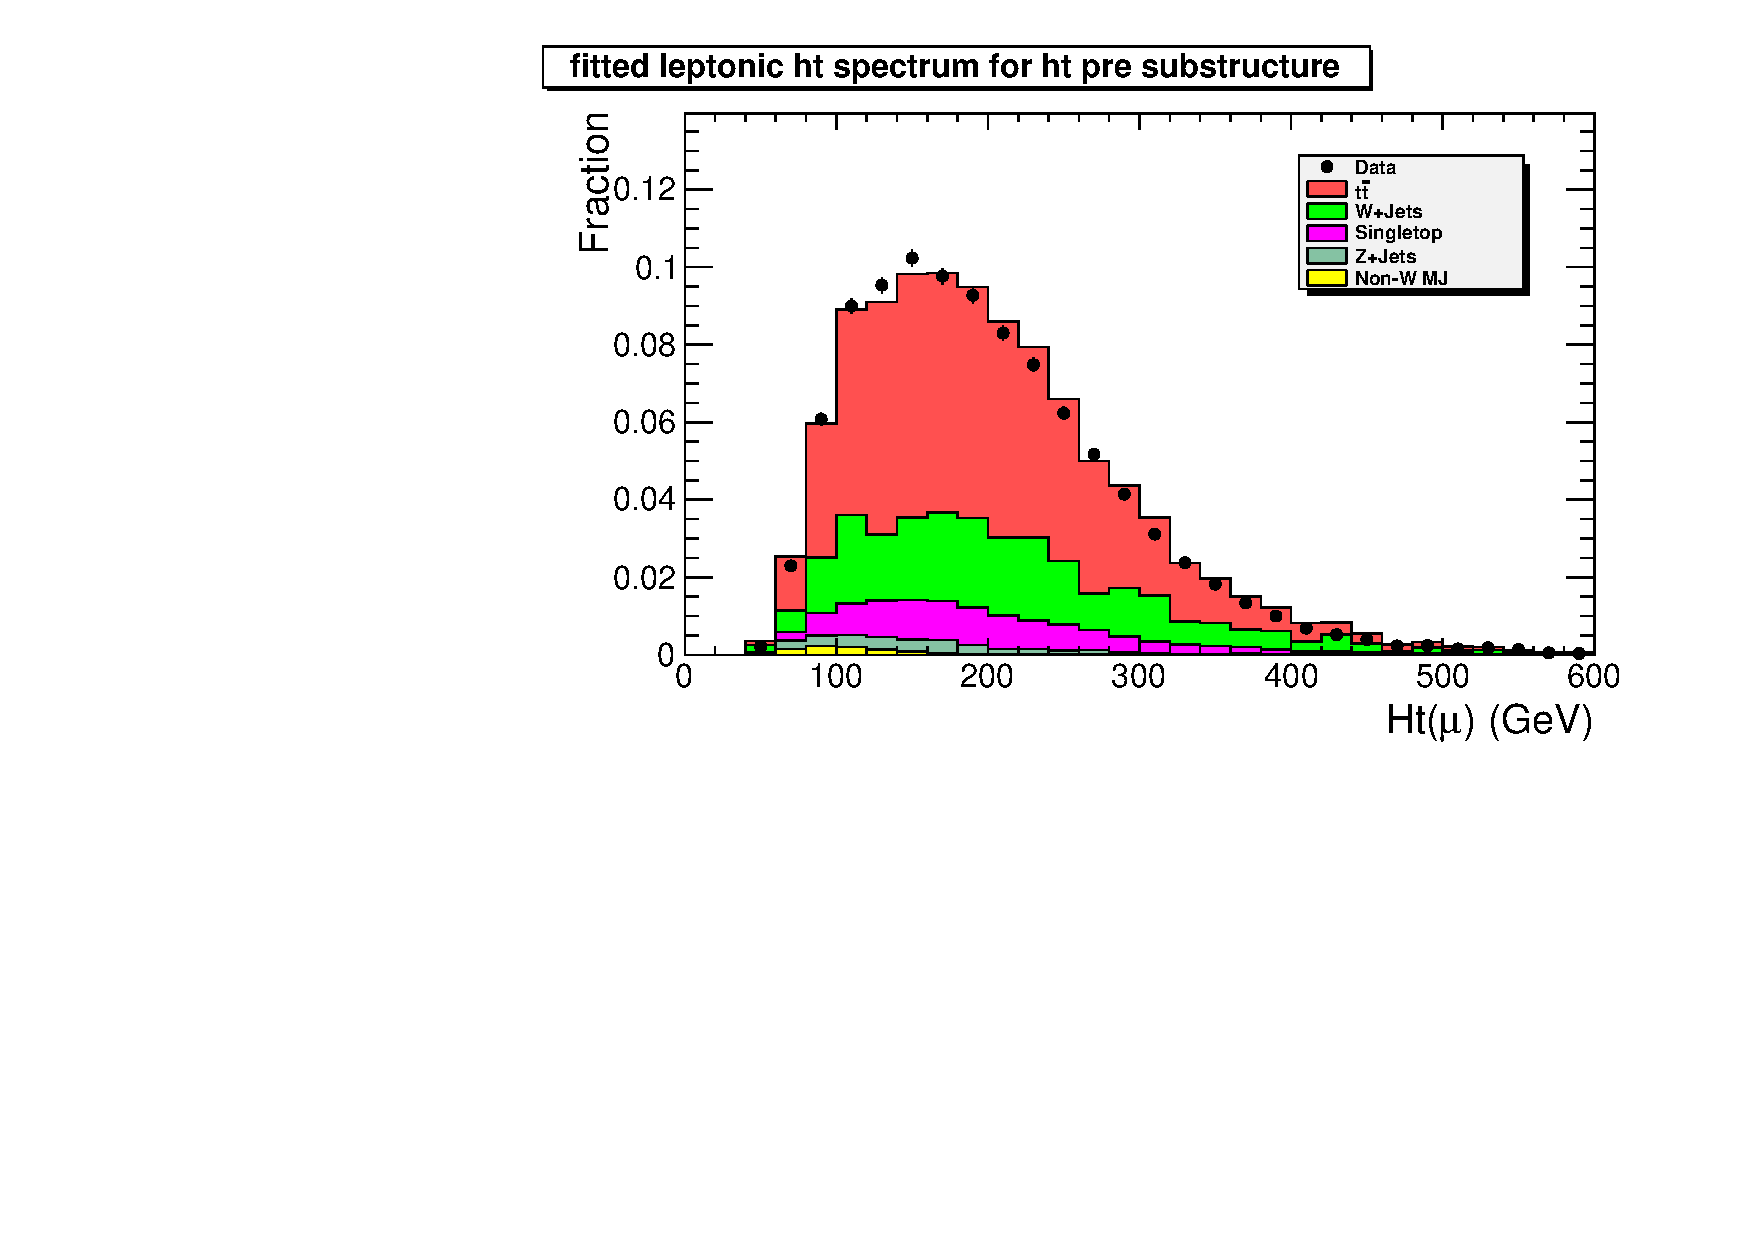
\includegraphics[width=1.0\textwidth]{figs/htLep3_comp.pdf}
\caption{Ht fit used to extract the fraction of QCD events.  This fit is performed before any substructure cuts are made.}
\label{figs:htLep3_comp}
\end{figure}


Figure ~\ref{figs:semiLepMass_mWCand} shows the highest mass jet in the hadronic hemisphere.  This jet is interpreted as originating in a W boson decay due to the
high purity of $\ttbar$ events from the previous selection.  The fits seen in figure ~\ref{figs:semiLepMass_mWCand} is a Gaussian on a very broad Guassian tail. 
The fit is performed
in both data the Monte Carlo, and from this fit we can extract the mean mass of the W boson ($M_W$).  We obtain the subjet energy scale factor by taking the 
ratio of 
$M_W$ derived from the background fit to the $M_W$ value extracted from the data fit.  From data we observe $M_W$ = 84.28$\pm$0.272 in Monte Carlo 
we observe $M_W$ = 83.662$\pm$0.164, which suggests a subjet scale factor of 1.007$\pm$0.004.

Figure ~\ref{figs:semiLepMass_muHist} shows the mass drop variable $\mu$ that is extracted from the jet pruning algorithm. From this plot we can extract the 
efficiency scale factor by measuring the ratio of efficiencies in data and Monte Carlo for a $\mu$ cut of $\mu < 0.4$.  The efficiency measured in data is 
0.498$\pm$0.003 and the efficiency measured in Monte Carlo gives 0.507$\pm$0.003, which suggests a scale factor of 0.982$\pm$0.008. From this sample, a top mass 
can be extracted by the pairwise mass of the W boson and the "closest jet" b candidate in the hadronic hemisphere described above.
The mass spectrum can be seen in figure ~\ref{figs:semiLepMass_mTopCand}.  From this, we can extract a scale factor for the W mass cut using the same procedure as 
the $\mu$ cut.
The efficiency from data is 0.550$\pm$0.004 and 0.583$\pm$0.004 from Monte Carlo.  The resulting scale factor is 0.944$\pm$0.010.  

Finally, the scale factor measurements from the $\mu$ and $M_W$ cuts are combined to give 0.927$\pm$0.013.  The type 2 scale factor is used to weight 
Monte Carlo type 2 top events in the full selection of the main analysis.

Additionally, The hadronic hemisphere can be used to extract type 1 top mass spectrum.  The cuts for this spectrum are in analogy to the main analysis.  
\begin{itemize}
\item Hadronic Hemisphere Selection
\begin{itemize}
\item Leading jet with $p_T > 400$ $\GeVc$
\item Leading jet Number of Subjets $> 2$
\item Leading jet is Minimum Pairwise mass  $> 50$ $\GeV$
\end{itemize}
\end{itemize}

The Minimum Pairwise Mass variable can be seen in figure ~\ref{figs:semiLepMass_t1MinimumPairwiseMass}, and the top mass can be seen 
in figure ~\ref{figs:semiLepMass_t1massprecut}. 
The efficiency in data for a Minimum Pairwise Mass cut of at least 50$\GeV$ is 0.607$\pm$0.017, and 0.670$\pm$0.016 for Monte Carlo giving a scale factor of 0.906$\pm$0.033.  
The efficiency for the top mass within a window of 140$\GeV$ and 250$\GeV$ in data is 0.910$\pm$0.013, and 0.890$\pm$0.013 in Monte Carlo giving a scale factor of 1.02$\pm$0.021.  
The overall scale factor for these cuts is then 0.926$\pm$ 0.039.  The type 1 scale factor is used to weight Monte Carlo type 1 top events in the full selection of the main analysis.

\begin{figure}[htcb]
\centering
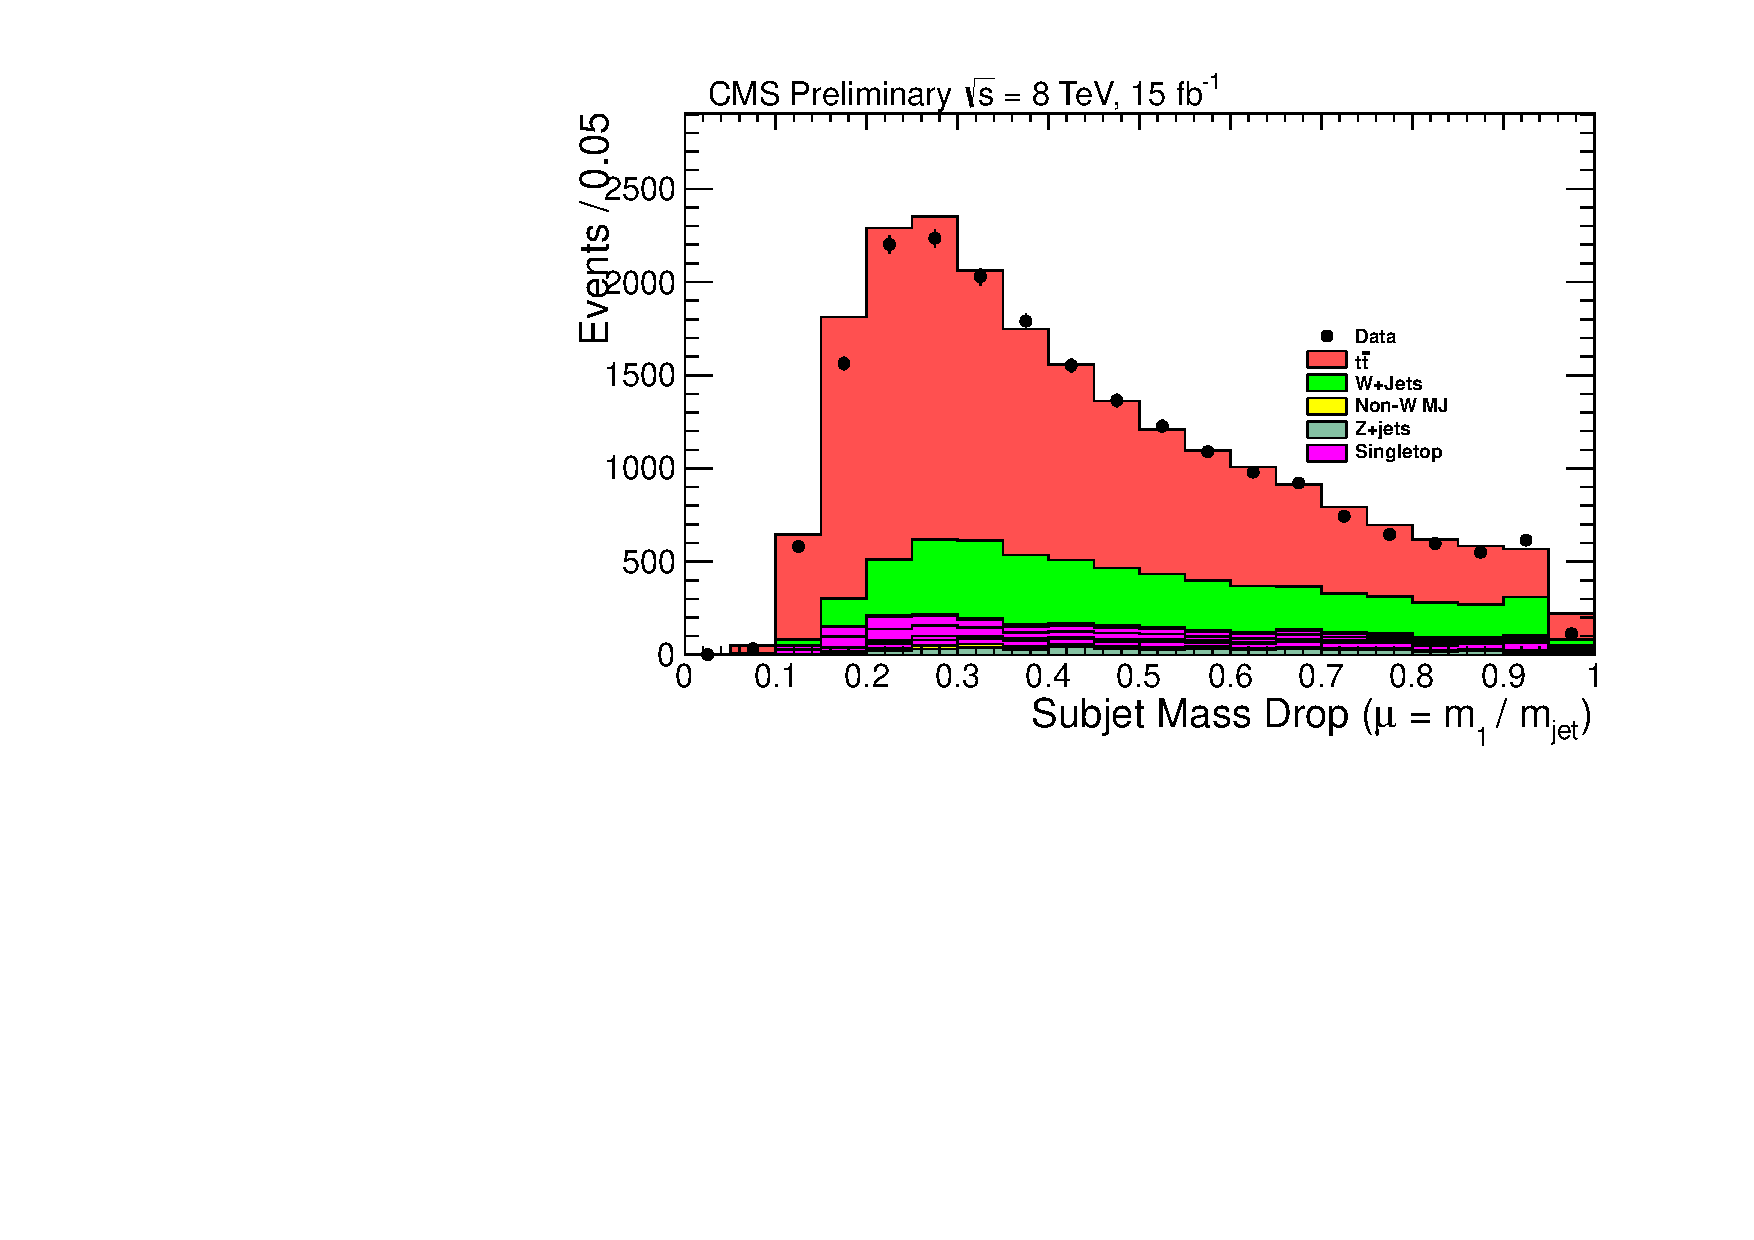
\includegraphics[width=1.0\textwidth]{figs/semiLepMass_muHist.pdf}
\caption{W candidate mass drop variable data and Monte Carlo Comparison.  The full selection for top mass requires a $\mu < 0.4$ cut.}
\label{figs:semiLepMass_muHist}
\end{figure}

\begin{figure}[htcb]
\centering
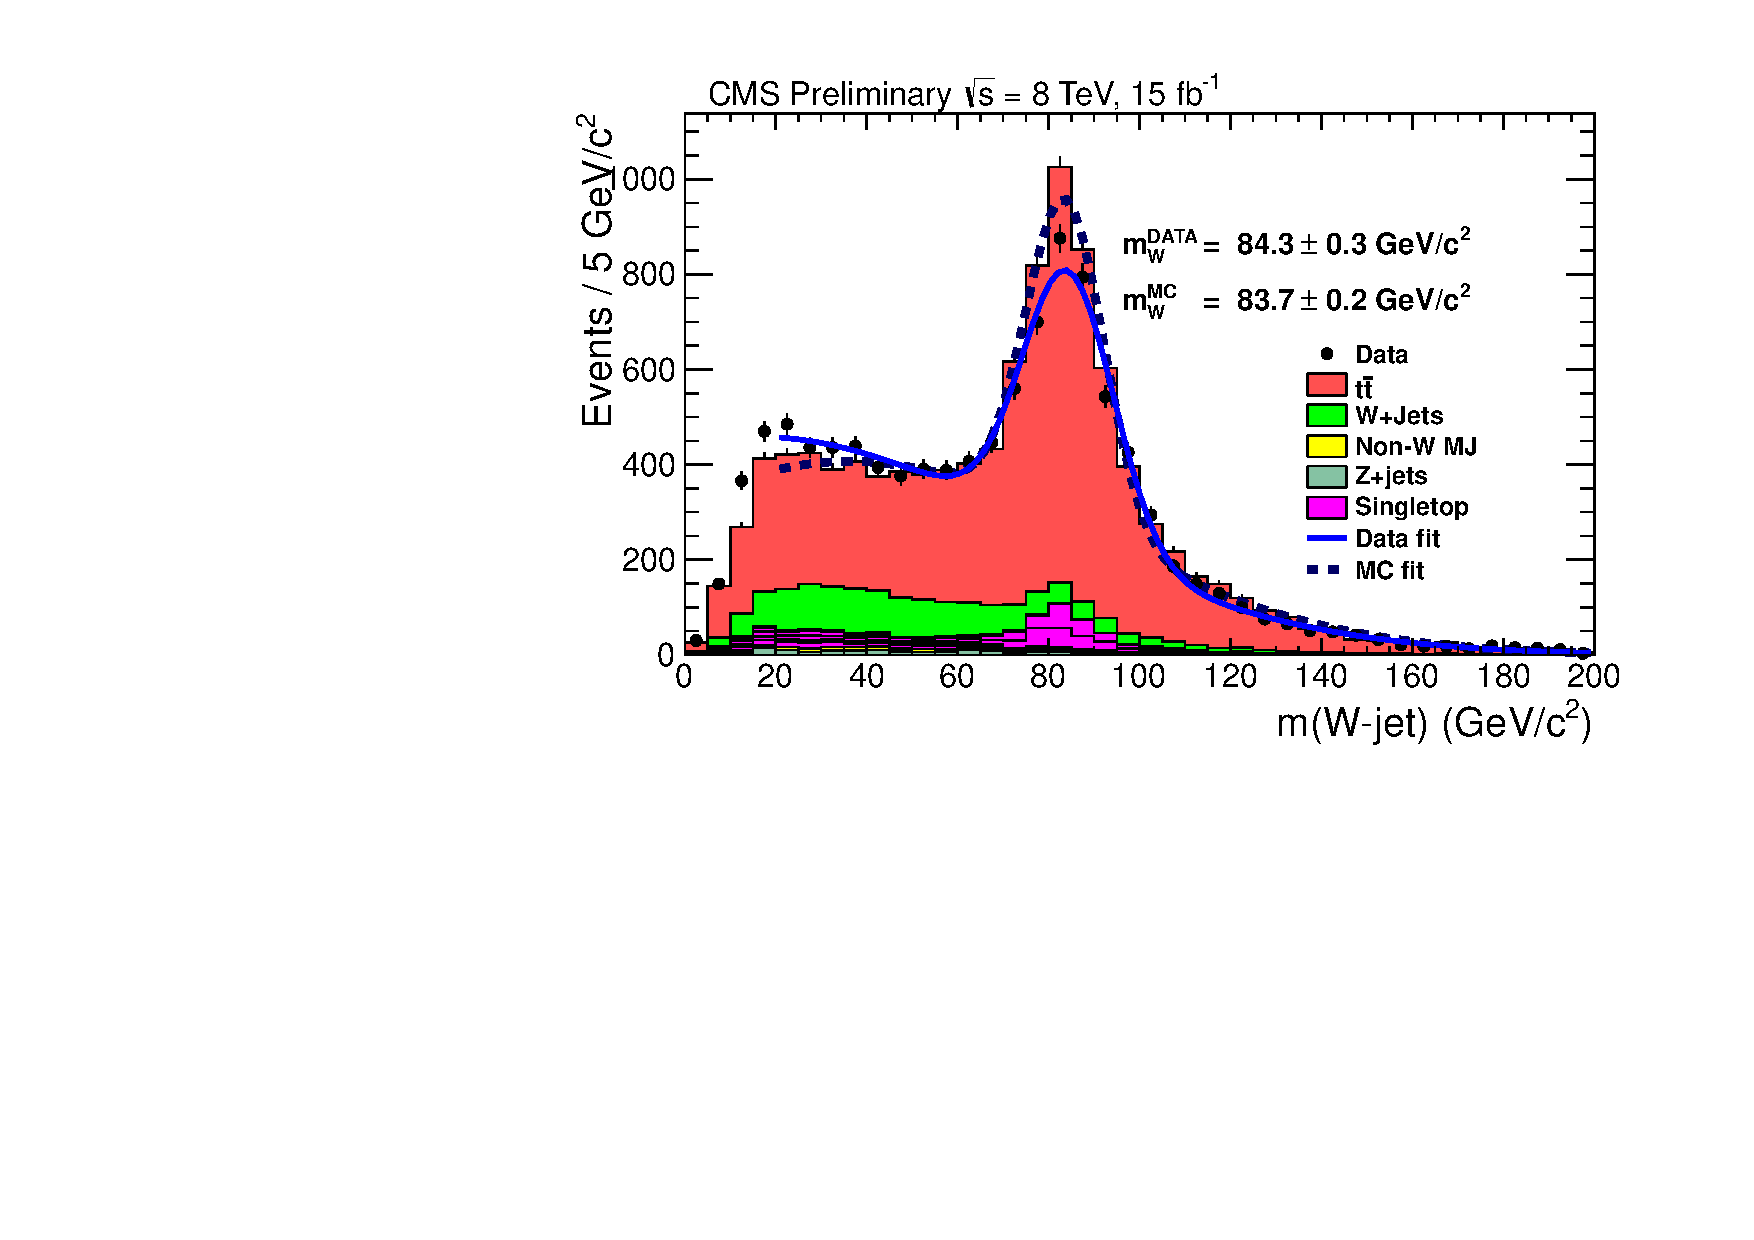
\includegraphics[width=1.0\textwidth]{figs/semiLepMass_mWCand.pdf}
\caption{W candidate mass data and Monte Carlo Comparison. The full selection for top mass requires a $60 < M_W < 130$ cut}
\label{figs:semiLepMass_mWCand}
\end{figure}

\begin{figure}[htcb]
\centering
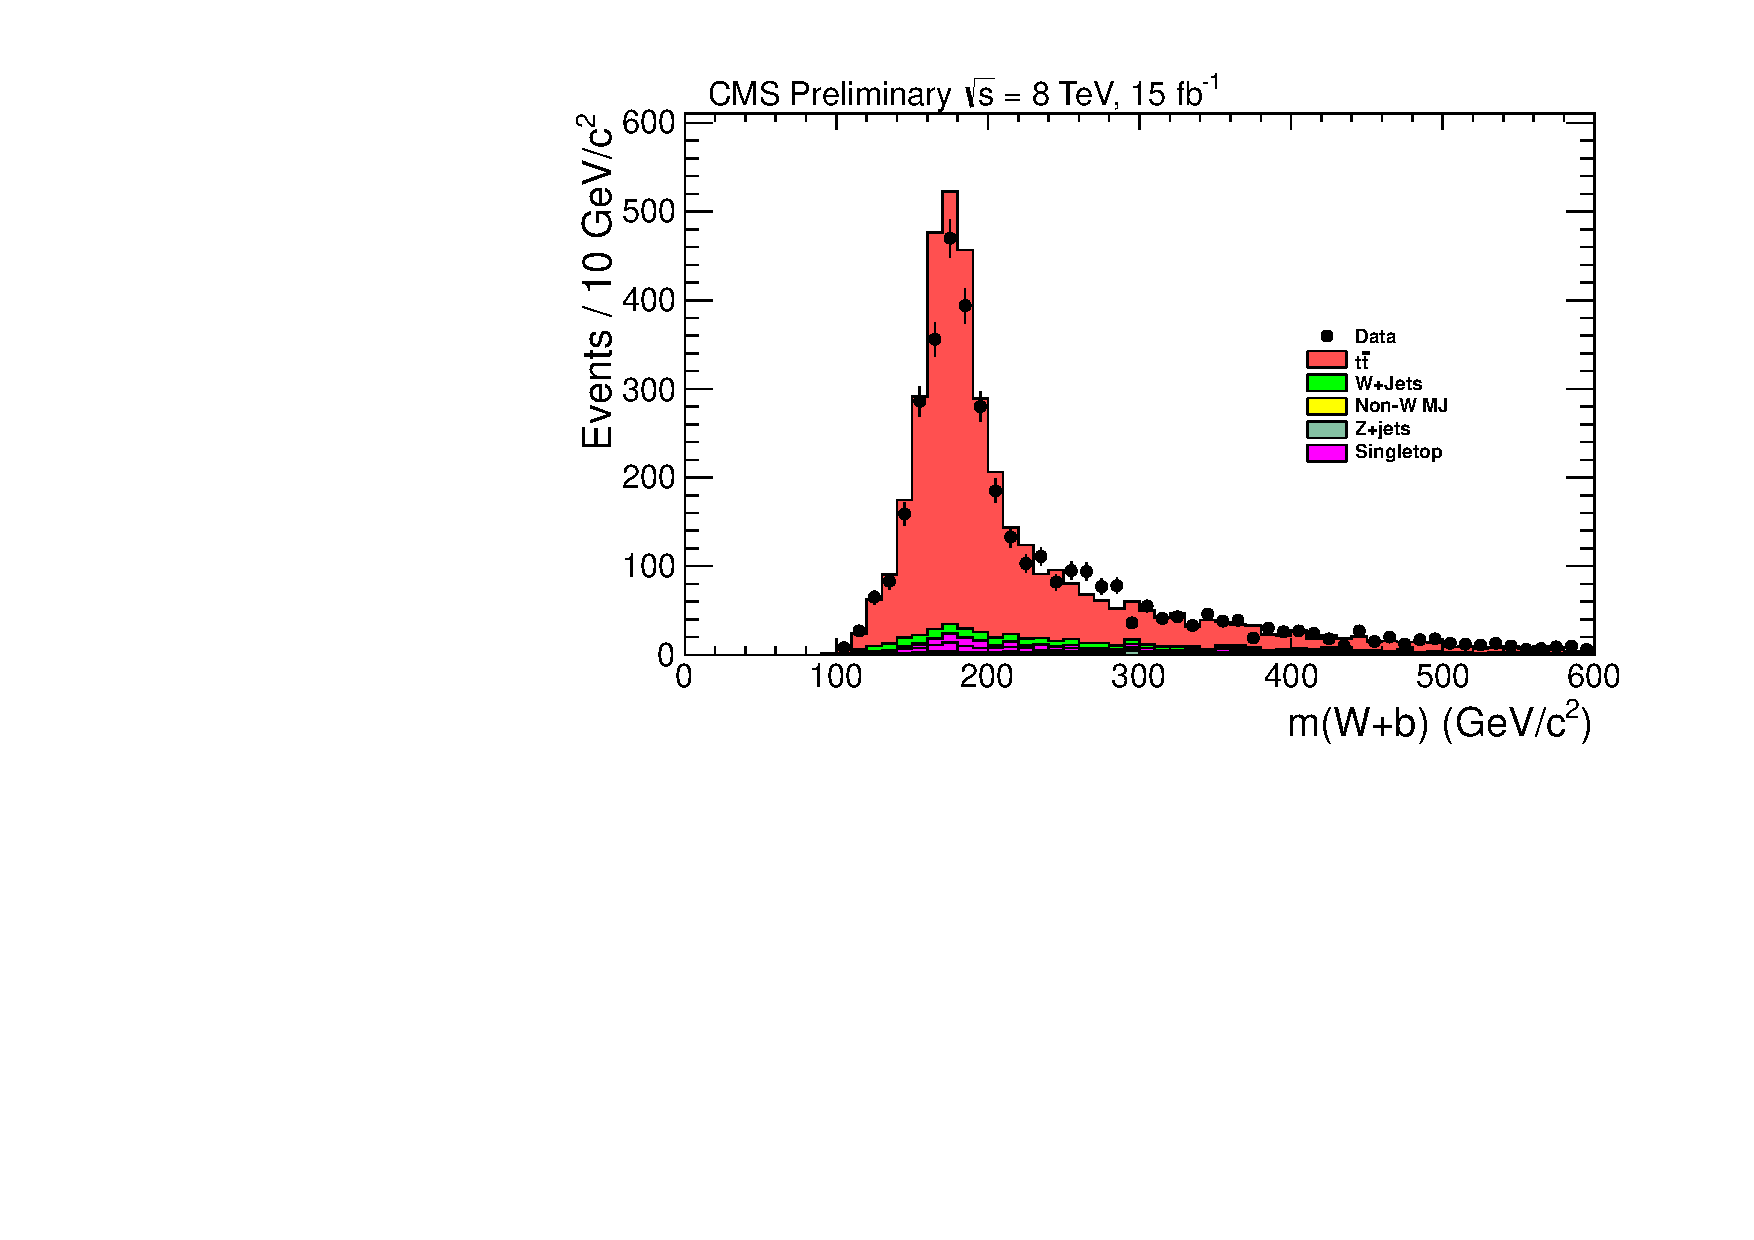
\includegraphics[width=1.0\textwidth]{figs/semiLepMass_mTopCand.pdf}
\caption{type 2 top candidate mass data and Monte Carlo Comparison}
\label{figs:semiLepMass_mTopCand}
\end{figure}

\begin{figure}[htcb]
\centering
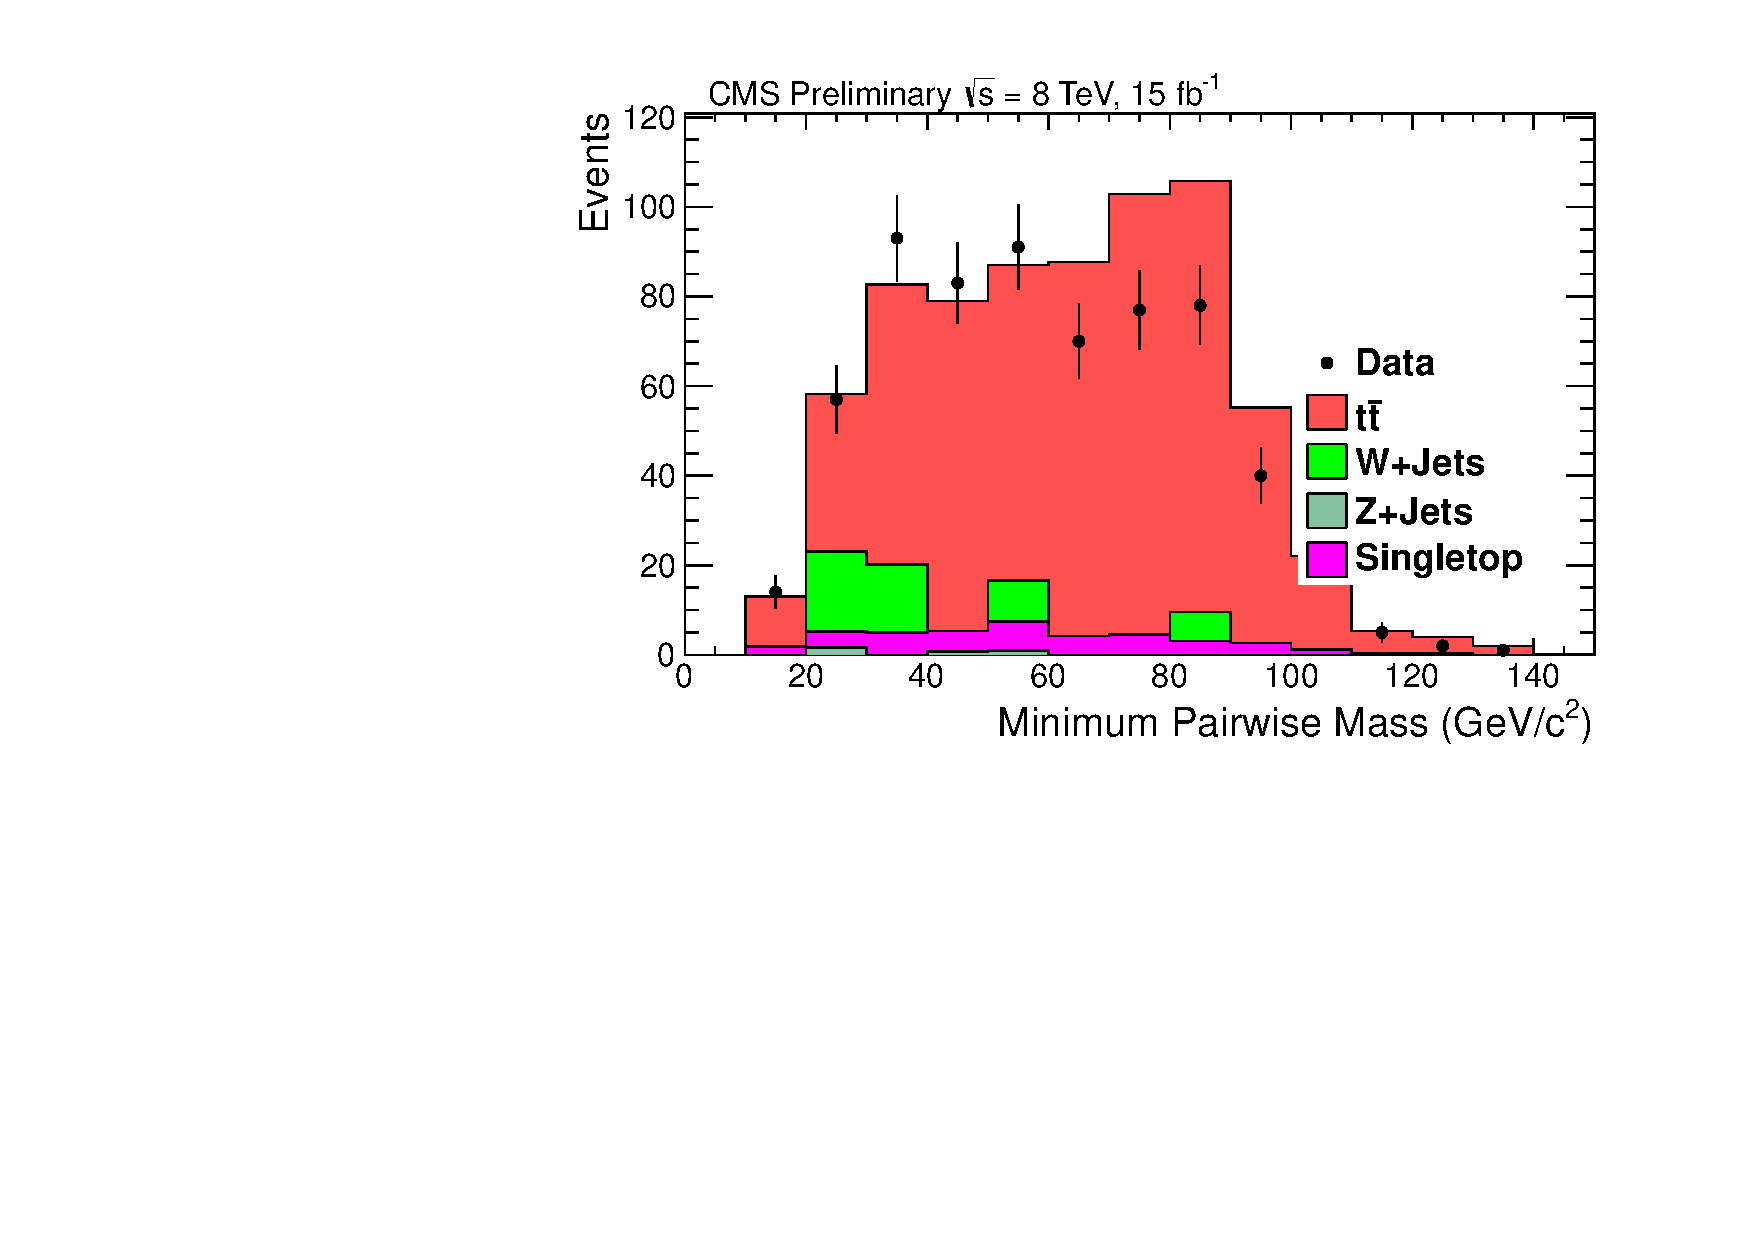
\includegraphics[width=1.0\textwidth]{figs/semiLepMass_t1MinimumPairwiseMass.pdf}
\caption{type 1 top candidate minimum pairwise mass data and Monte Carlo Comparison}
\label{figs:semiLepMass_t1MinimumPairwiseMass}
\end{figure}
\clearpage

\begin{figure}[htcb]
\centering
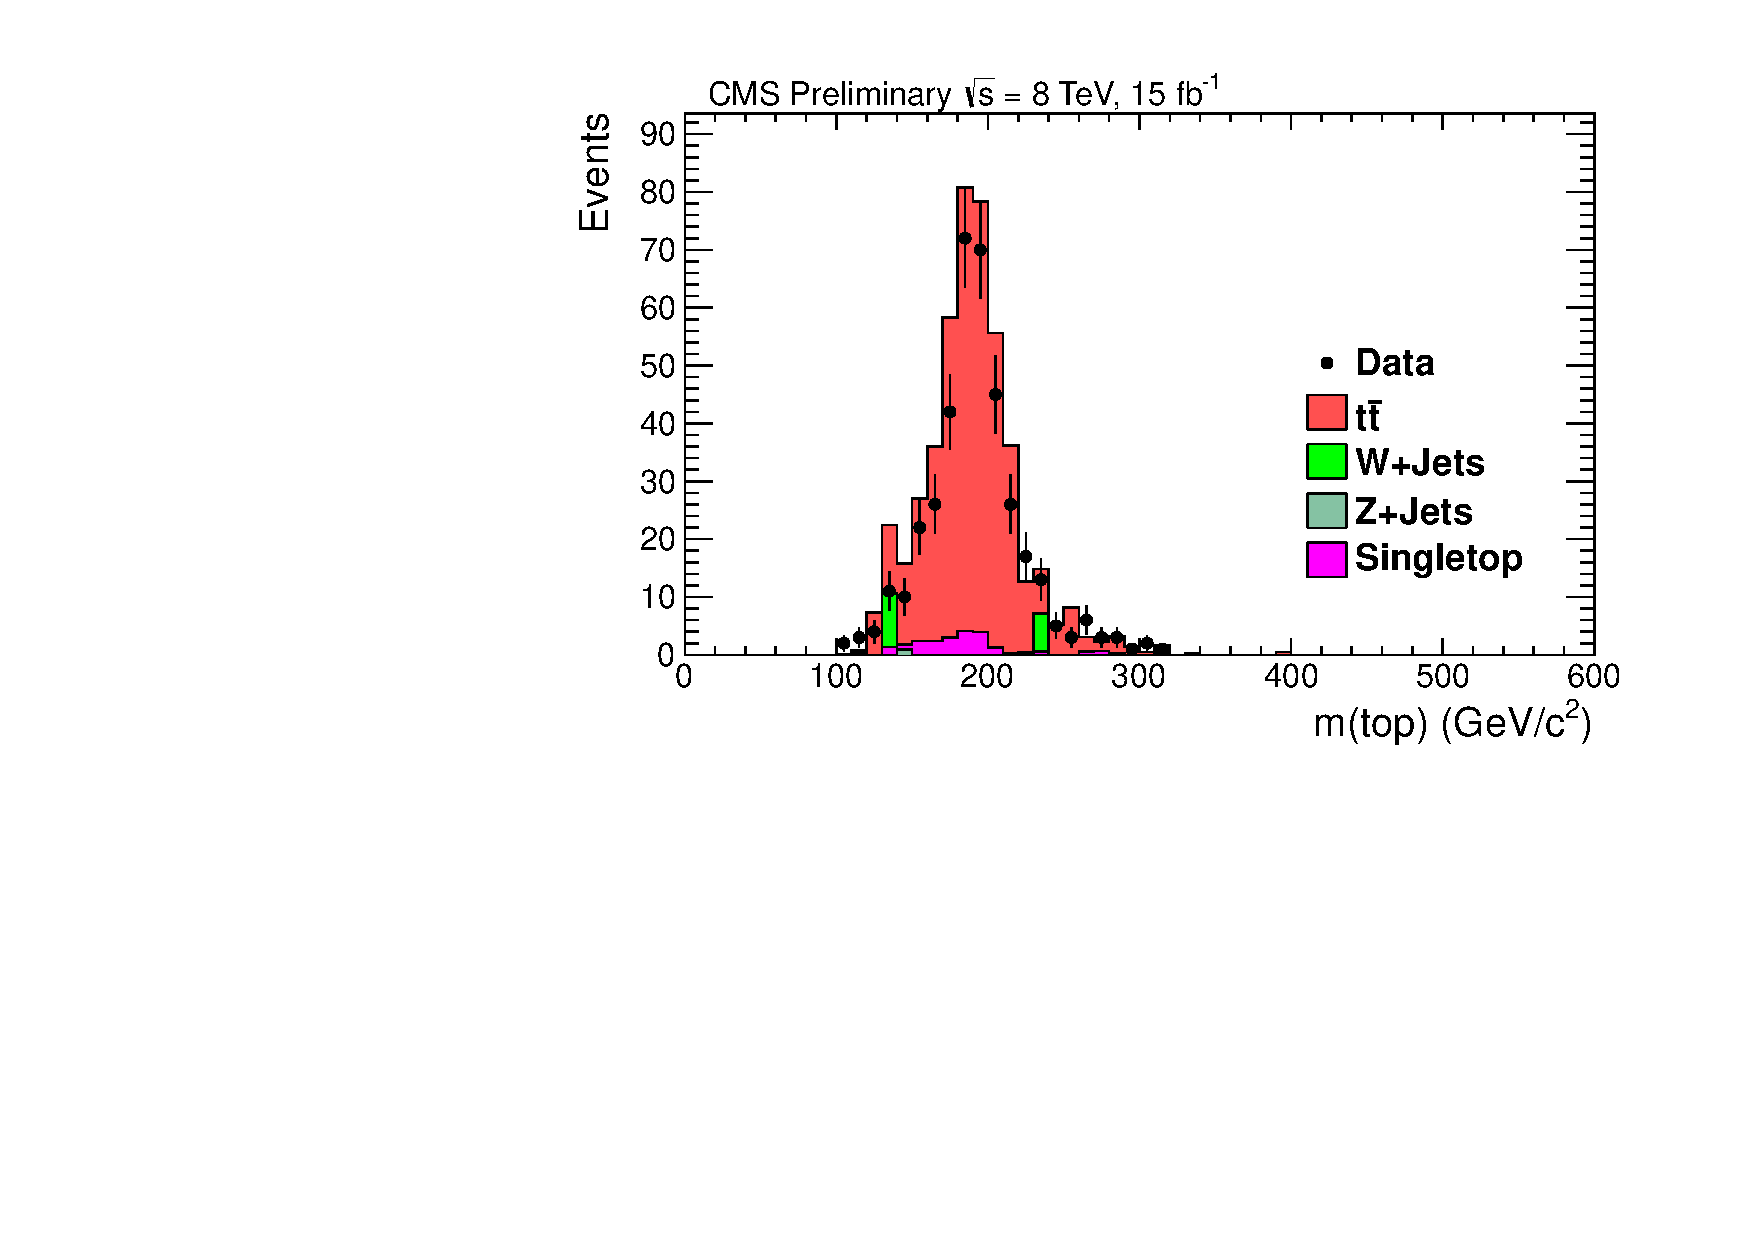
\includegraphics[width=1.0\textwidth]{figs/semiLepMass_t1TopMass.pdf}
\caption{type 1 top candidate mass data and Monte Carlo Comparison}
\label{figs:semiLepMass_t1massprecut}
\end{figure}
\clearpage

\clearpage
\newpage
\chapter{Background Estimation}
\label{sec:backgroundEstimation}
An essential part of the analysis is the data driven estimation of the QCD background.  
The background estimate relies on extracting the average b-tagging rate of a QCD jet in our signal region.  
We extract this rate by making use of the following sideband.
\section{Substructure Sideband}
\label{sec:sideband}
We define the substructure sideband as events passing all signal region cuts but explicitly 
failing the top jet substructure cut on the number of subjets.  Additionally, to ensure similar parton flavor distributions in the signal region and sideband (Figure \ref{figs:partonflav}), 
we also include subjet CSV discrimination. The top jet sideband is defined as:
\begin{eqnarray}
	140  <  m_{\text{jet}}  <  250 \GeV \\
	N_{\text{subjets}}  \leq  2 \\
	SJ_{\text{CSVMAX}} \geq 0.679 
\end{eqnarray}
The Minimum Pairwise Mass variable described in Section \ref{sec:toptagging} is not defined in this choice of sideband.

\section{QCD Background Estimation}
\label{sec:qcdBackgroundEstimationProcedure}
\label{sec:tagrateparameterization}
The estimation of QCD background is performed by extracting the probability to tag a b jet in the sideband. 
The primary assumption used in background estimation is that the average b-tagging probability 
for QCD multijets in the signal region is nearly identical to the sideband. Figure \ref{figs:partonflav}  shows the parton flavor distribution for signal region and sideband in QCD MC, the
 nearly identical composition can be considered motivation for the previous assumption.

To extract a QCD background estimate, we weight the events that pass the full selection in the signal region before the b-tagging requirement is applied by 
the average b-tagging probability (measured in the top jet sideband).  This gives us an accurate expectation of the QCD background in the signal region.
The b-tagging rate is defined as the inverse ratio of the number of b candidate jets, 
defined as $\pt > 370~\GeV$ jets in the hemisphere opposite the top jet to the number of b candidate jets that are b-tagged.  
%This ratio is shown if Figure \ref{figs:partonflav} in bins of parton flavor for signal region and sideband as extracted from QCD Monte Carlo.    

\begin{figure}[htbp]
\begin{center}
\subfigure{\label{figs:partonflavCOMP}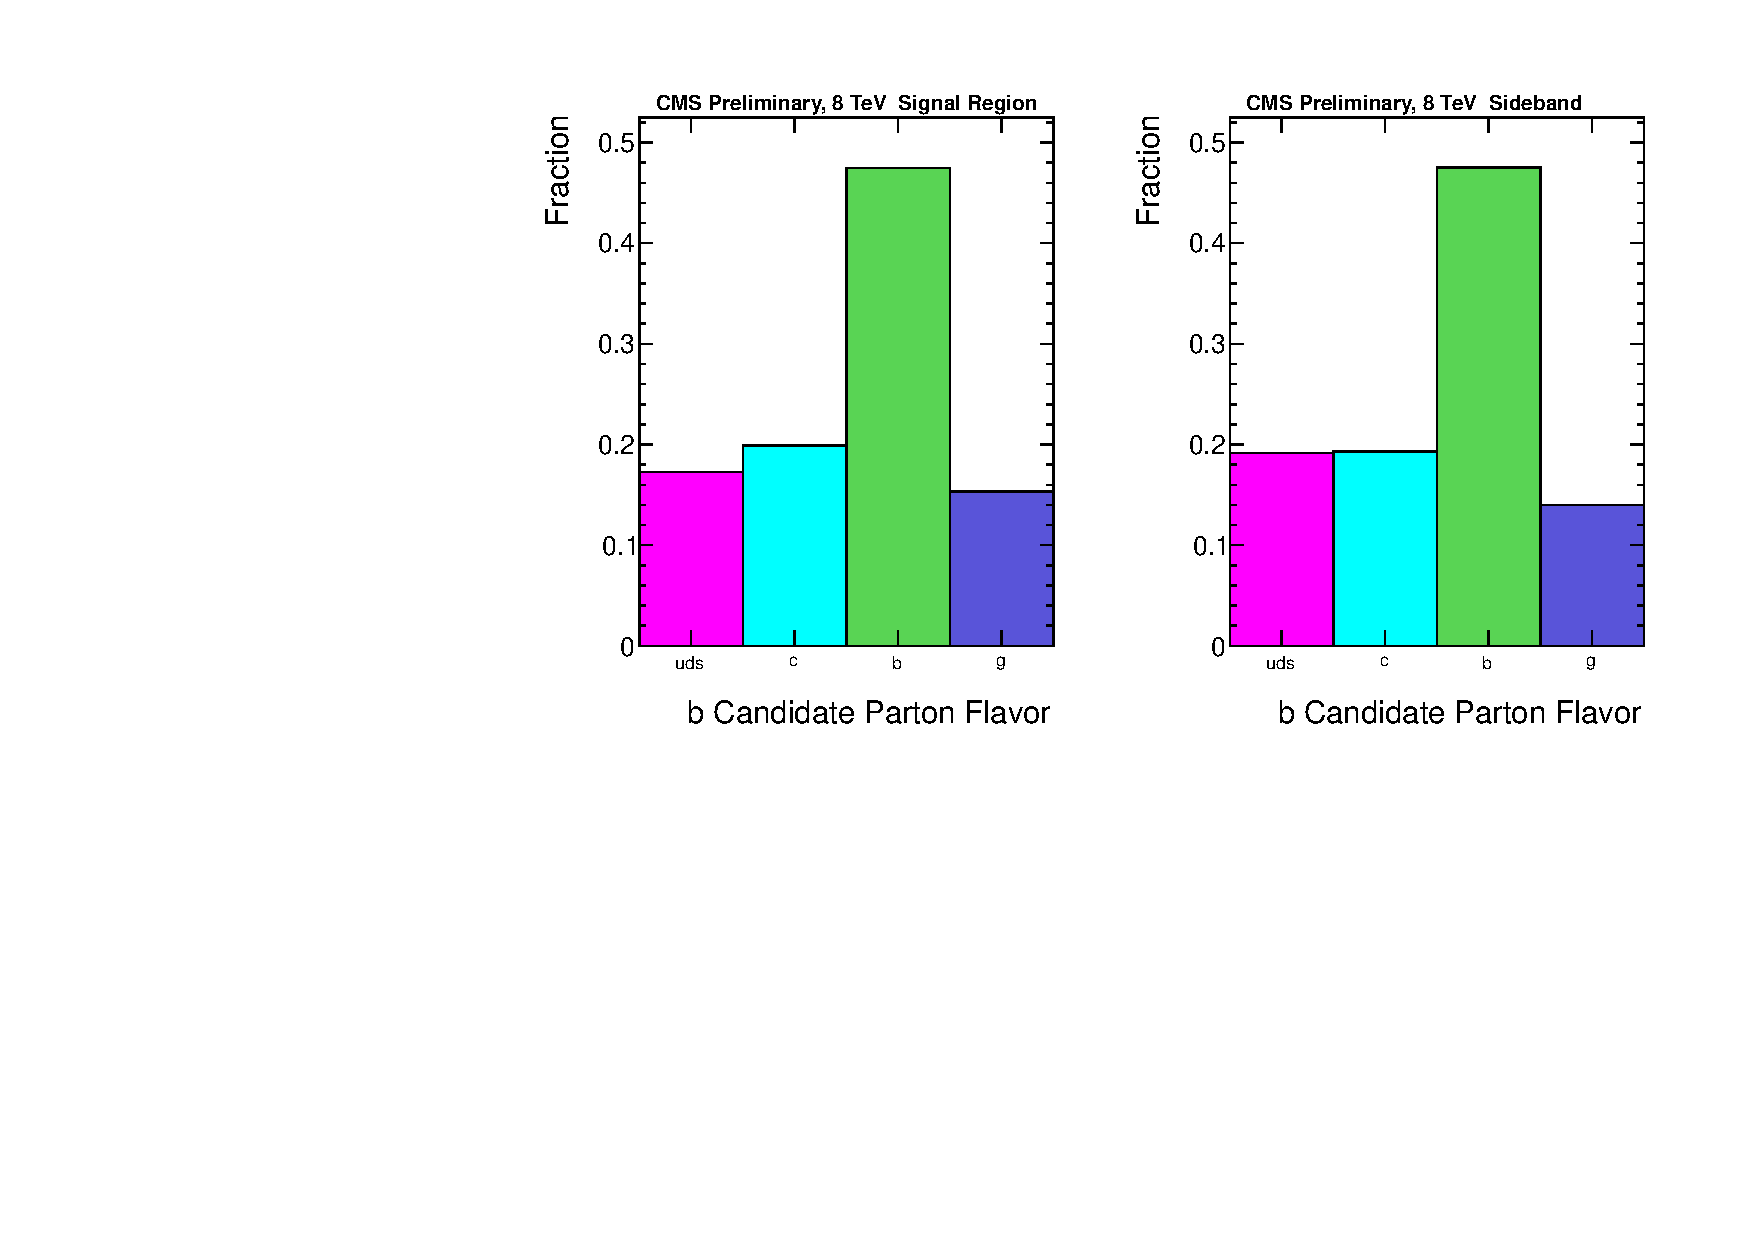
\includegraphics[width=1.0\textwidth]{AN-13-004/figs/partonflavCOMP}}\\ 
\caption{
Comparison of jet parton flavor composition from the signal region and sideband.
%(b) Comparison of average b-tagging rate as a function of jet parton flavor from the signal region and sideband.  
}
\label{figs:partonflav}
\end{center}
\end{figure}

The parameterization of the average b-tagging rate is two dimensional and considers both the $|\eta|$ and $\pt$ of the b candidate jets.  
We break down data into three distinct regions in $|\eta|$. 


\begin{itemize}
	\item \text{Low } $(0.0 < |\eta| \leq 0.5)$
	\item \text{Transition } $(0.5 < |\eta| \leq 1.15)$ 
	\item \text{High } $(1.15 < |\eta| \leq 2.4)$ 
\end{itemize}

The regions in $|\eta|$ are then individually parameterized in $\pt$ to produce the average b-tagging rate.  We perform this parameterization 
of the b-tagging rate in an attempt to constrain the kinematic correlations inherent in b-tagging.

To smooth out the binning of the average b-tagging rate, a study of functional fits was conducted for the average b-tagging rate (see Figure \ref{figs:BKGFITCOMP}).
We chose the bifurcated polynomial fit based on observed representation of the data.  The fitting function is as follows

\begin{eqnarray}
f(x) =
\begin{cases}
p_0+p_1x+p_2(x-\text{a})^2, & \text{if x} < \text{a} \\
p_0+p_1x+p_3(x-\text{a})^2, & \text{if x}\geq\text{a}
\end{cases}
\end{eqnarray}

Here, the parameters $p_0$ through $p_3$ are inputs to the fitting algorithm, and x is the $\pt$ of the b candidate jet.  The parameter a is the bifurcation point, and is chosen manually for each region in $\eta$.
It is chosen to be 500$~\GeV$, 500$~\GeV$, and 550$~\GeV$ for the low, transition, and high $\eta$ regions respectively.
This piecewise function allows for two characteristic ranges to fit a polynomial, which makes a good fit for the different functional forms of the average b-tagging rate regions that we use.

The errors on the average b-tagging rate are then extracted using the full covariance matrix as obtained from output of the fitting 
algorithm.   
Additionally, we assign a systematic uncertainty to cover the choice of the fit function (see Chapter \ref{sec:systematics}) based on several alternative functional forms.
Figure \ref{figs:tagsandprobes8TeV} shows the tags (numerator) and probes (denominator) of the tagging rate.
Figure \ref{figs:tagrateetafit} shows the three fitted average b-tagging rates parameterized in $\pt$.  

%\section{Treatment of QCD Background Events with Double Top Tags}
%\label{sec:dubtags}
%As mentioned in Section \ref{sec:analysisStrategy}, the analysis uses  hemispherically separated dijets as top and b candidates.  
%Because it is not obvious which candidate will be the leading jet, both are considered.  If the event registers a count in either of these configurations, the other is not considered to prevent double counting.  
%However, the QCD background estimate is based on the probability of recording a count and thus the cut to prevent double counting should not be applied when filling the QCD background.  
%This type of event occurs when both the leading and sub leading jet are top tagged, and both jets are considered for b-tagging.  
%Note that this does not impact the treatment of ttbar, and these events are simply of rare QCD origin (see Section \ref{sec:ttSubtraction}). 
%An event that records two counts in the background estimation has the physical meaning that the event has two chances to tag a b jet.

\section{$\ttbar$ Subtraction}
\label{sec:ttSubtraction}
\label{sec:bsttSubtraction}
The $\ttbar$ contribution to background is computed from Monte Carlo that passes the full selection. To avoid double-counting, we must remove $\ttbar$ from our QCD estimate. 
In creating the b-tagging rate, the $\ttbar$ contribution to the numerator and denominator is subtracted away using $\ttbar$ Monte Carlo. 
Additionally, we account for the $\ttbar$ contamination of the QCD background estimate by applying 
the average b-tagging rate to $\ttbar$ Monte Carlo in the same way as data.  This is a measure of $\ttbar$ that is expected to fall 
through the QCD background estimate and is subtracted away. 

%We can similarly consider the possible effect of the single-top contribution to this tag rate. 
%However, due to the very low background from single-top, we find that we do not need to modify the average b-tagging rate. 
%Table \ref{table:singletop} shows a comparison of the various contribution to the average b-tagging rate.  
%Theoretically, the signal could also be present in the 
%pre tagged and post tagged sample, which could bias the background estimation.  However, in practice it is seen that this effect is a fraction of a 
%percent and is thus much smaller than the uncertainty placed on the background estimation.

\begin{table}
\begin{center}
\begin{tabular}{|c||c|c|c|} 
\hline
  & $\eta_1$ & $\eta_2$ & $\eta_3$ \\
\hline
\hline
pretag QCD & 15922 ($99.77\%$) & 14396 ($99.79\%$) & 5494 ($99.81\%$)\\
tagged QCD & 924 ($99.17\%$) & 847 ($99.16\%$) & 285 ($99.54\%$)\\
pretag $\ttbar$ & 37 ($0.23\%$) & 31 ($0.21\%$) & 11 ($0.19\%$)\\
tagged $\ttbar$ & 8 ($0.83\%$) & 7 ($0.84\%$) & 1 ($0.46\%$)\\
pretag signal at 1300$\GeV$ & 108 ($0.67\%$) & 77 ($0.53\%$) & 17 ($0.30\%$)\\
tagged signal at 1300$\GeV$ & 37 ($3.94\%$) & 24 ($2.87\%$) & 4 ($1.44\%$)\\
pretag signal at 1500$\GeV$ & 62 ($0.39\%$) & 39 ($0.27\%$) & 8 ($0.14\%$)\\
tagged signal at 1500$\GeV$ & 17 ($1.86\%$) & 11 ($1.28\%$) & 2 ($0.67\%$)\\
pretag signal at 1700$\GeV$ & 31 ($0.19\%$) & 19 ($0.13\%$) & 3 ($0.06\%$)\\
tagged signal at 1700$\GeV$ & 8 ($0.82\%$) & 4 ($0.53\%$) & 1 ($0.25\%$)\\
pretag signal at 1900$\GeV$ & 15 ($0.09\%$) & 9 ($0.06\%$) & 1 ($0.02\%$)\\
tagged signal at 1900$\GeV$ & 3 ($0.31\%$) & 2 ($0.20\%$) & 0 ($0.07\%$)\\
pretag signal at 2100$\GeV$ & 7 ($0.04\%$) & 4 ($0.03\%$) & 0 ($0.01\%$)\\
tagged signal at 2100$\GeV$ & 1 ($0.13\%$) & 1 ($0.09\%$) & 0 ($0.03\%$)\\
\hline
\end{tabular}
\end{center}
\caption{Number of tagged and pretagged events for each background sample and percent contribution to overall average b-tagging rates.  Additionally, signal samples are investigated.  
The percents indicated are out of the total QCD + $\ttbar$ expectation and the signal samples are scaled to theory cross-section.}
\label{table:singletop}
\end{table}

\begin{figure}[htcb]
\centering
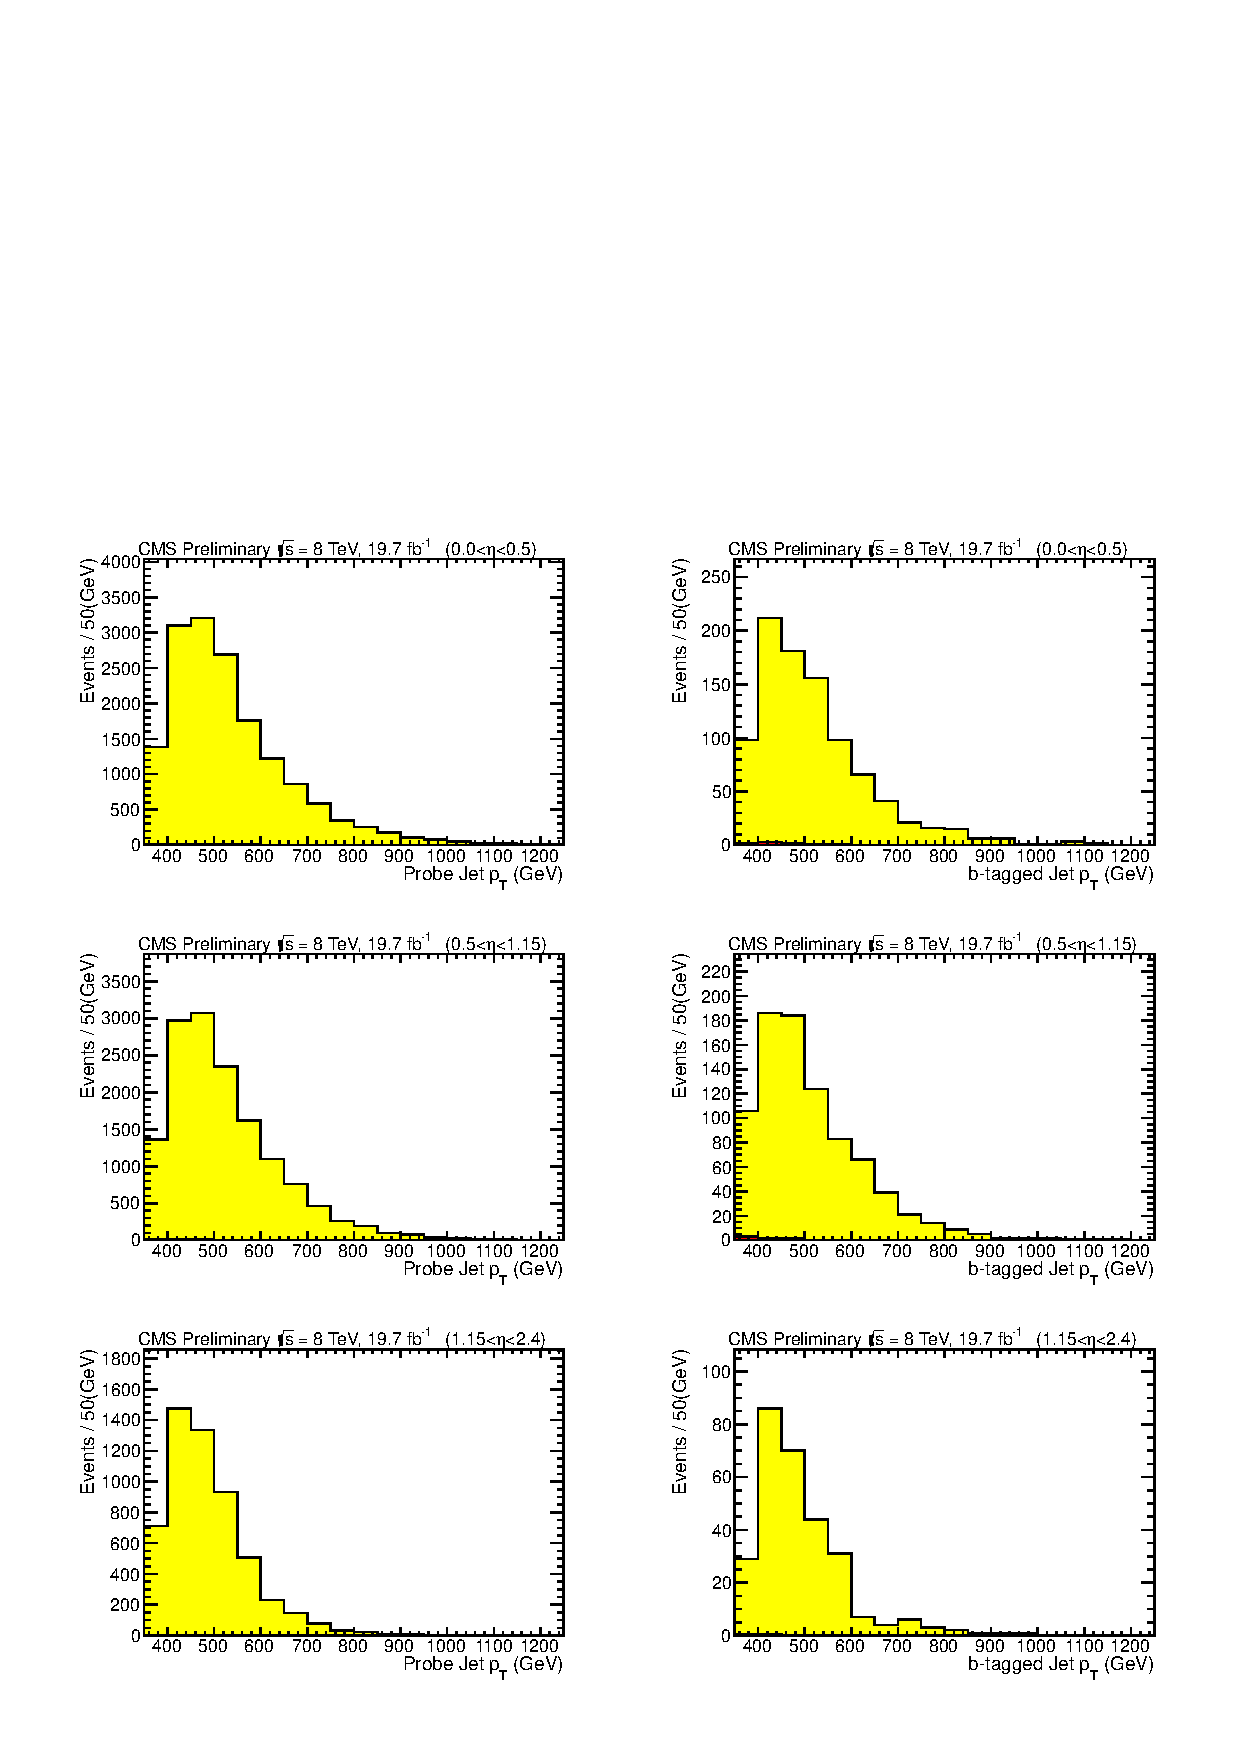
\includegraphics[width=1.0\textwidth]{AN-13-004/figs/tagsandprobes}
\caption{The tags and probes used for the average b-tagging rate in each of the three regions in $|\eta|$ .  Here, tags are the numerator and probes are the denominator of the average b-tagging rate}
\label{figs:tagsandprobes8TeV}
\end{figure}

\begin{figure}[htcb]
\begin{center}
\subfigure{\label{figs:tagrateeta1fit}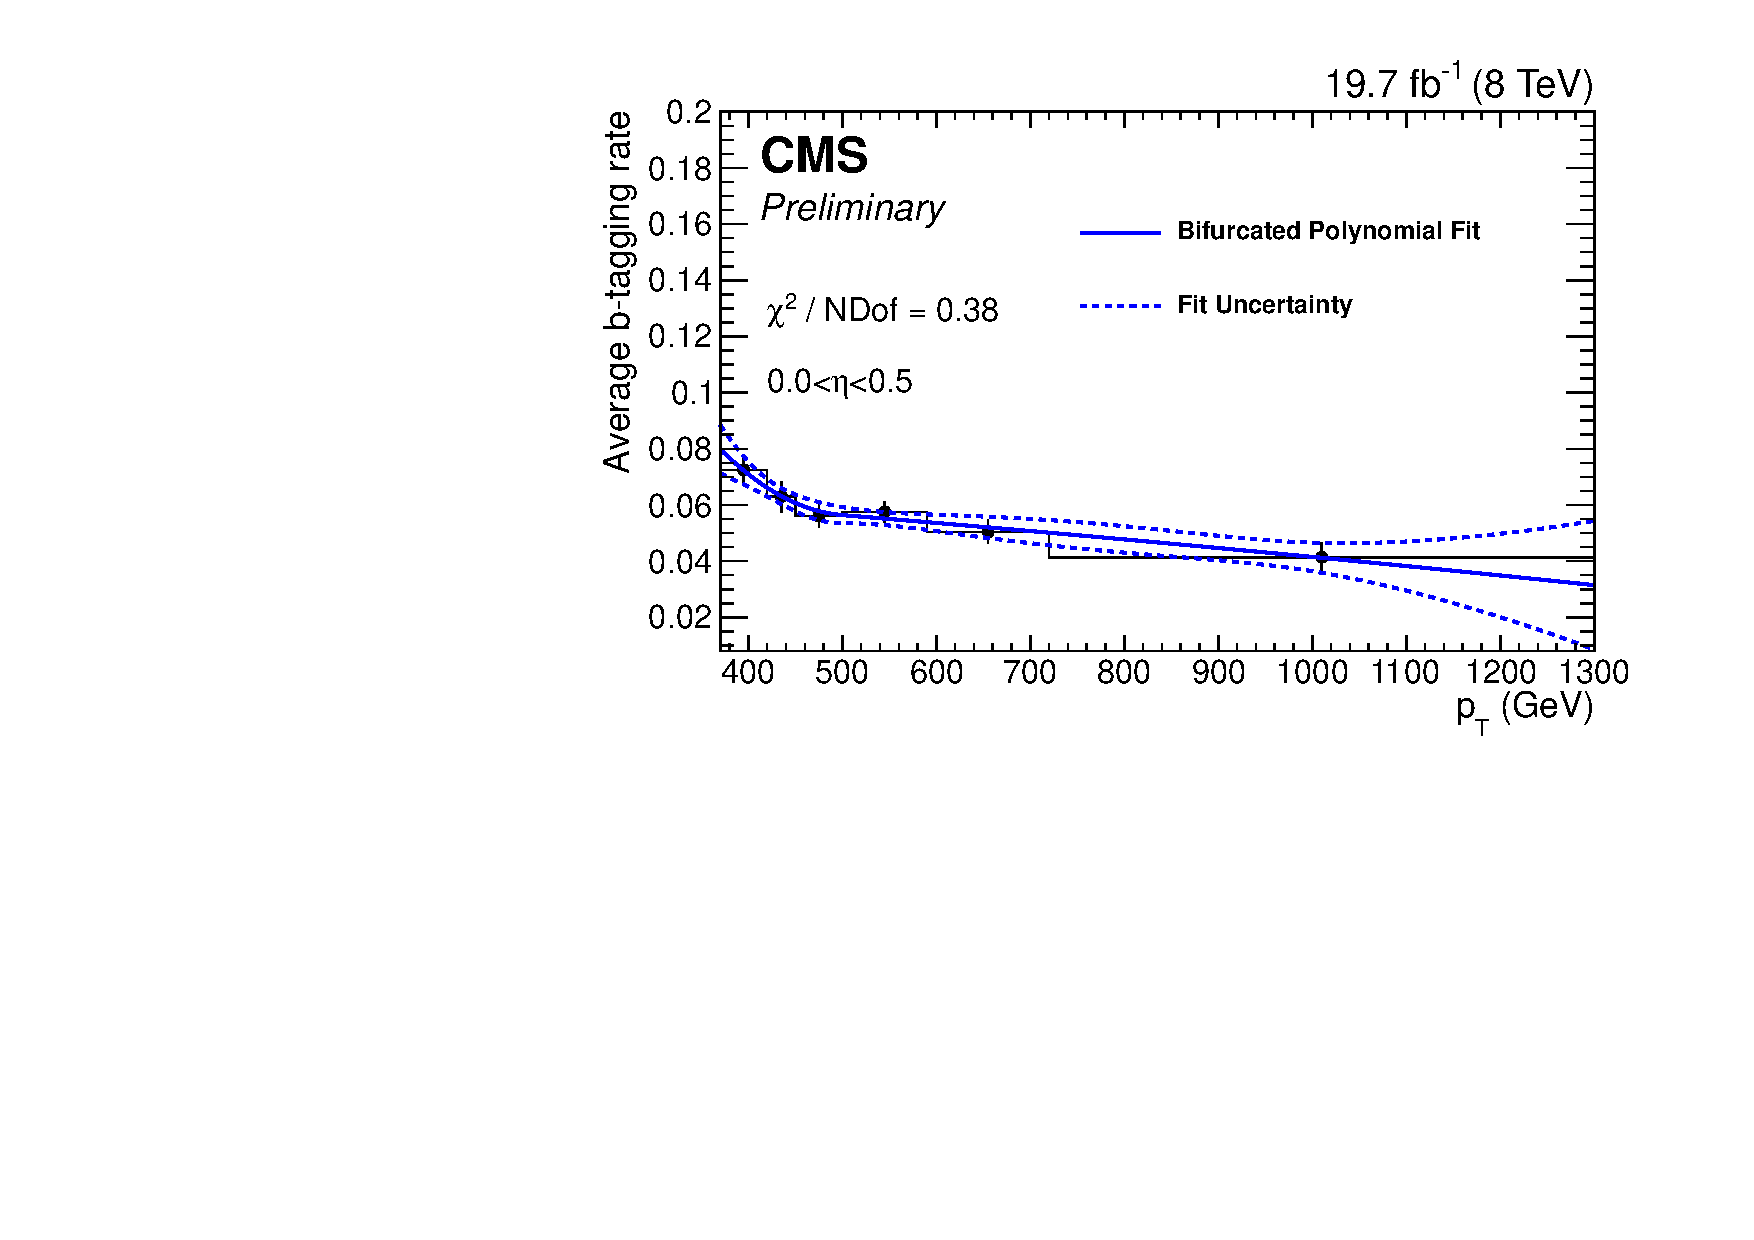
\includegraphics[width=0.7\textwidth]{AN-13-004/figs/tagrateeta1fitBP.pdf}}\\
\subfigure{\label{figs:tagrateeta2fit}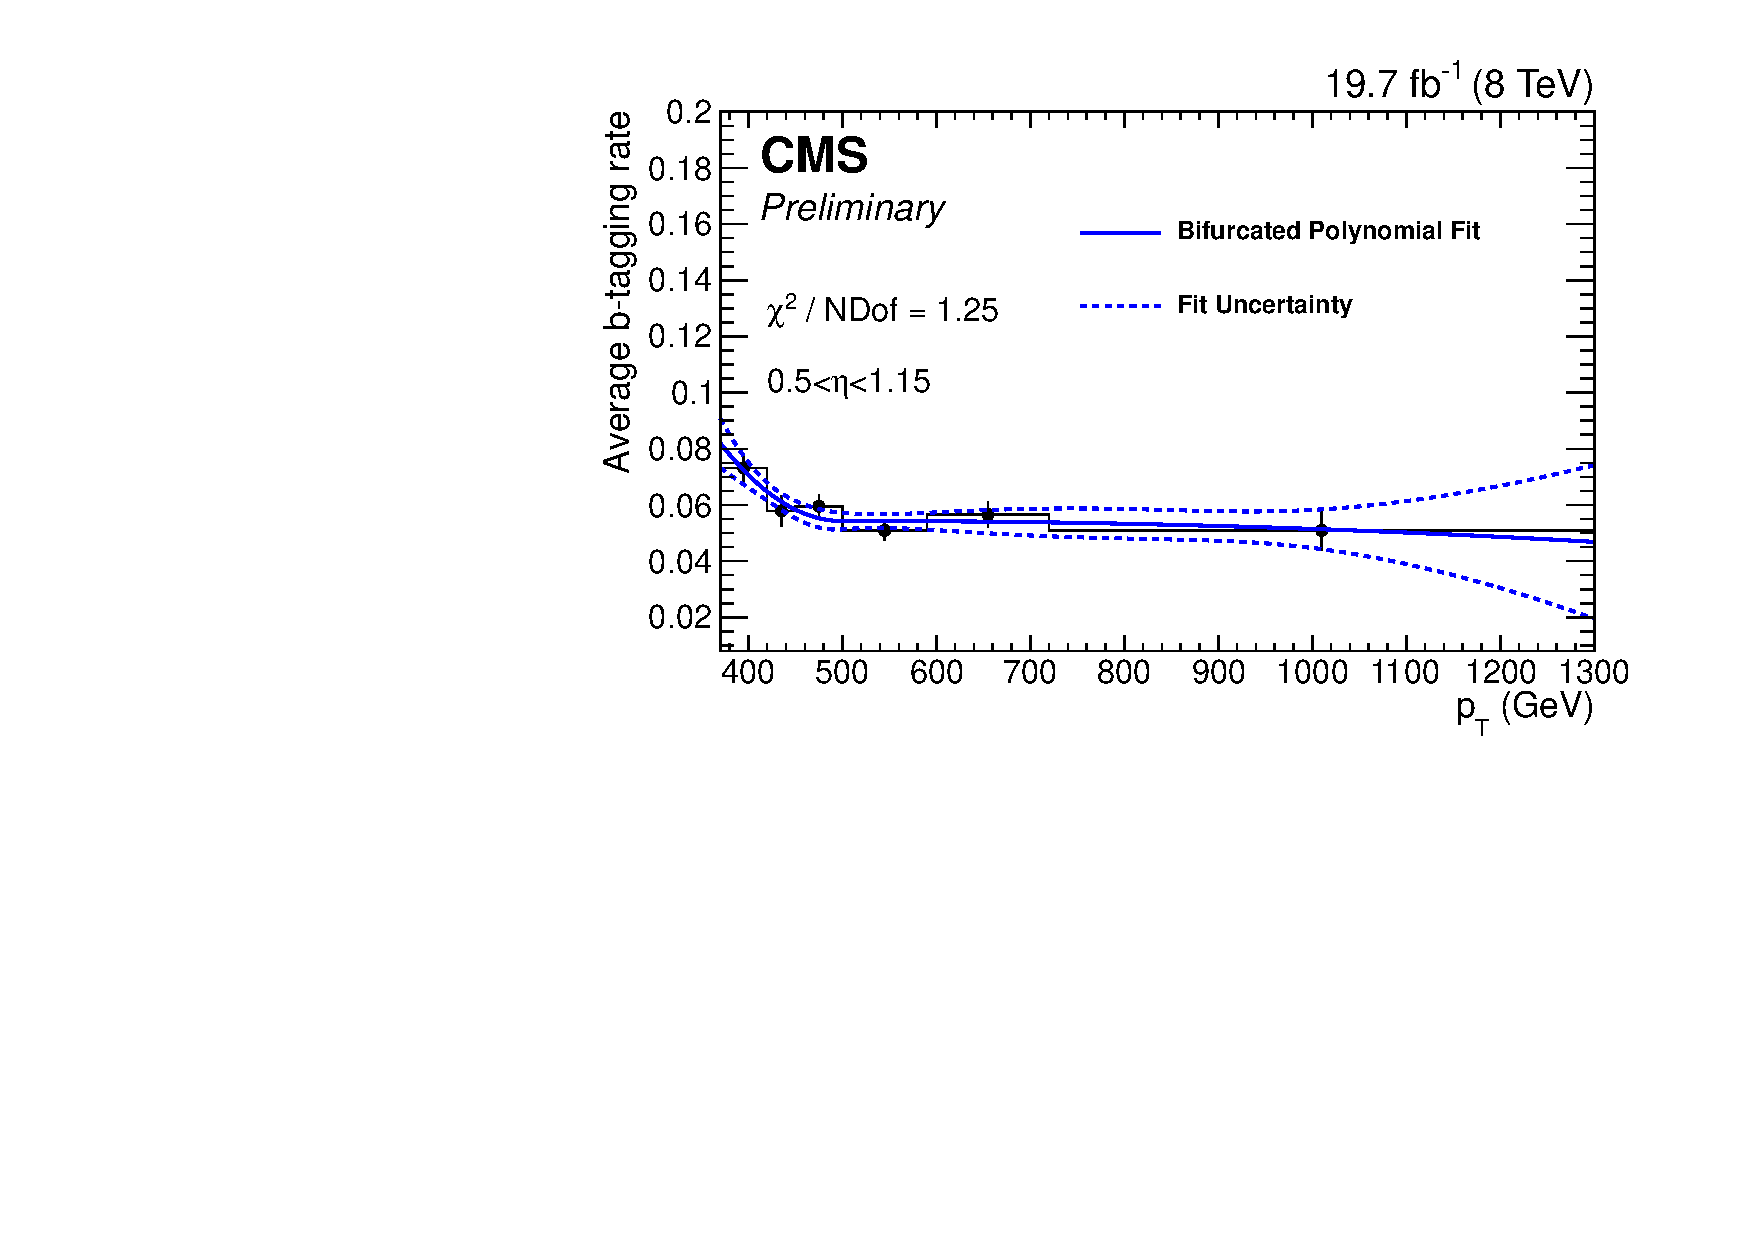
\includegraphics[width=0.7\textwidth]{AN-13-004/figs/tagrateeta2fitBP.pdf}}\\
\subfigure{\label{figs:tagrateeta3fit}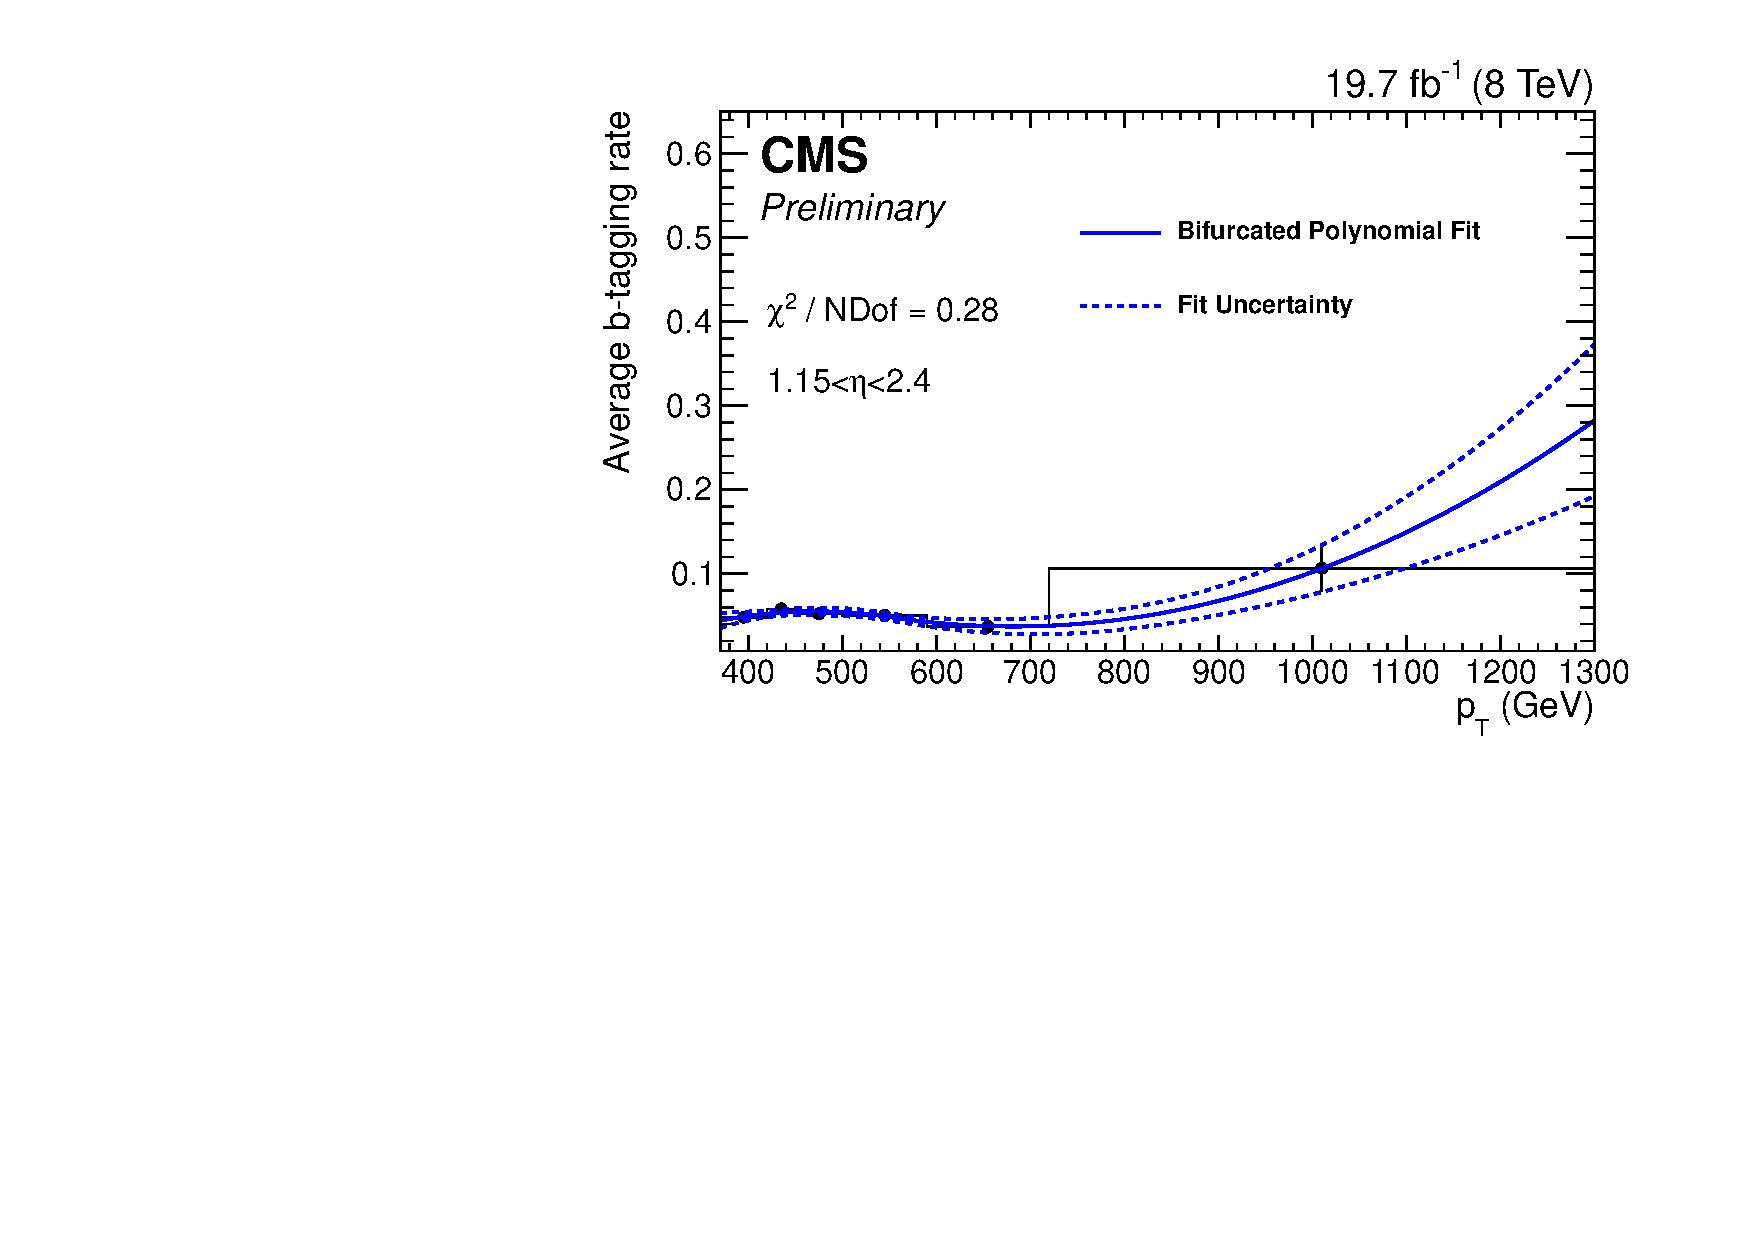
\includegraphics[width=0.7\textwidth]{AN-13-004/figs/tagrateeta3fitBP.pdf}}
\caption{
$\pt$ parameterized average b-tagging rate from
(a) Low $\eta$ region  
(b) Transition $\eta$ region 
(c) High $\eta$ region. 
  The average b-tagging rate is shown in black, the polynomial fit is shown in blue, and the propagated errors from the fit are shown as a blue dashed line.}
\label{figs:tagrateetafit}
\end{center}
\end{figure}

%\section{QCD Closure}
%As a closure test, the background estimation is performed on the QCD Monte Carlo samples listed in Table \ref{table:datasetsQCD}.  

%\begin{table}
%\begin{center}
%\begin{tabular}{|p{0.7\linewidth}|r|} 
%\hline
%\bf{Sample} & \bf{Cross-Section} \\
%\hline
%/QCD\_Pt-300to470\_TuneZ2star\_8TeV\_pythia6/Summer12-PU\_S7\_START52\_V9-v1/AODSIM & 1759.6 \\
%/QCD\_Pt-470to600\_TuneZ2star\_8TeV\_pythia6/Summer12-PU\_S7\_START52\_V9-v1/AODSIM & 113.9 \\
%/QCD\_Pt-600to800\_TuneZ2star\_8TeV\_pythia6/Summer12-PU\_S7\_START52\_V9-v1/AODSIM & 27.0 \\
%/QCD\_Pt-800to1000\_TuneZ2star\_8TeV\_pythia6/Summer12-PU\_S7\_START52\_V9-v1/AODSIM & 3.57 \\
%/QCD\_Pt-1000to1400\_TuneZ2star\_8TeV\_pythia6/Summer12-PU\_S7\_START52\_V9-v1/AODSIM & 0.738 \\
%/QCD\_Pt-1400to1800\_TuneZ2star\_8TeV\_pythia6/Summer12-PU\_S7\_START52\_V9-v1/AODSIM & 0.0335 \\
%\hline
%\end{tabular}
%\end{center}
%\caption{QCD Monte Carlo Sample.}
%\label{table:datasetsQCD}
%\end{table}

%The extracted tagrates are shown in Figure\ref{figs:tagrateetafitQCD}.  
%Here, the tagrate was extracted with the procedure noted in Sections \ref{sec:qcdBackgroundEstimationProcedure} 
%and \ref{sec:tagrateparameterization}, as the $\ttbar$ contribution is not present here.  The closure test was performed by using the tagrates to weigh 
%pre b tagged jets within the relevant $|\eta|$ and $\pt$ regions with the tagrate as fitted with the bifurcated polynomial fit outlined in Section \ref{sec:tagrateparameterization}.  For this closure test, 
%the tagrates were extracted from the sideband using only even numbered events from the Monte Carlo and applied to only the odd numbered events in the signal region.  
%The results are shown in Figure\ref{figs:QCDClosure}.    
%The Monte Carlo here is scaled to the total number of events in our full selection in data, and the error bars represent 
%$\sqrt{N}$ where N is the bin content.  This procedure allows us to investigate the effect of any possible bias given the current integrated luminosity.  The QCD closure analysis performed on the full statistic QCD sample can be seen in 
%\ref{figs:QCDClosure1}.  
%The tagrate comparison of signal region and sideband is shown in Figure\ref{figs:tagrateetaQCD_withSR}

%\begin{figure}[htcb]
%\begin{center}
%\subfigure{\label{figs:tagrateeta1fitBPQCD}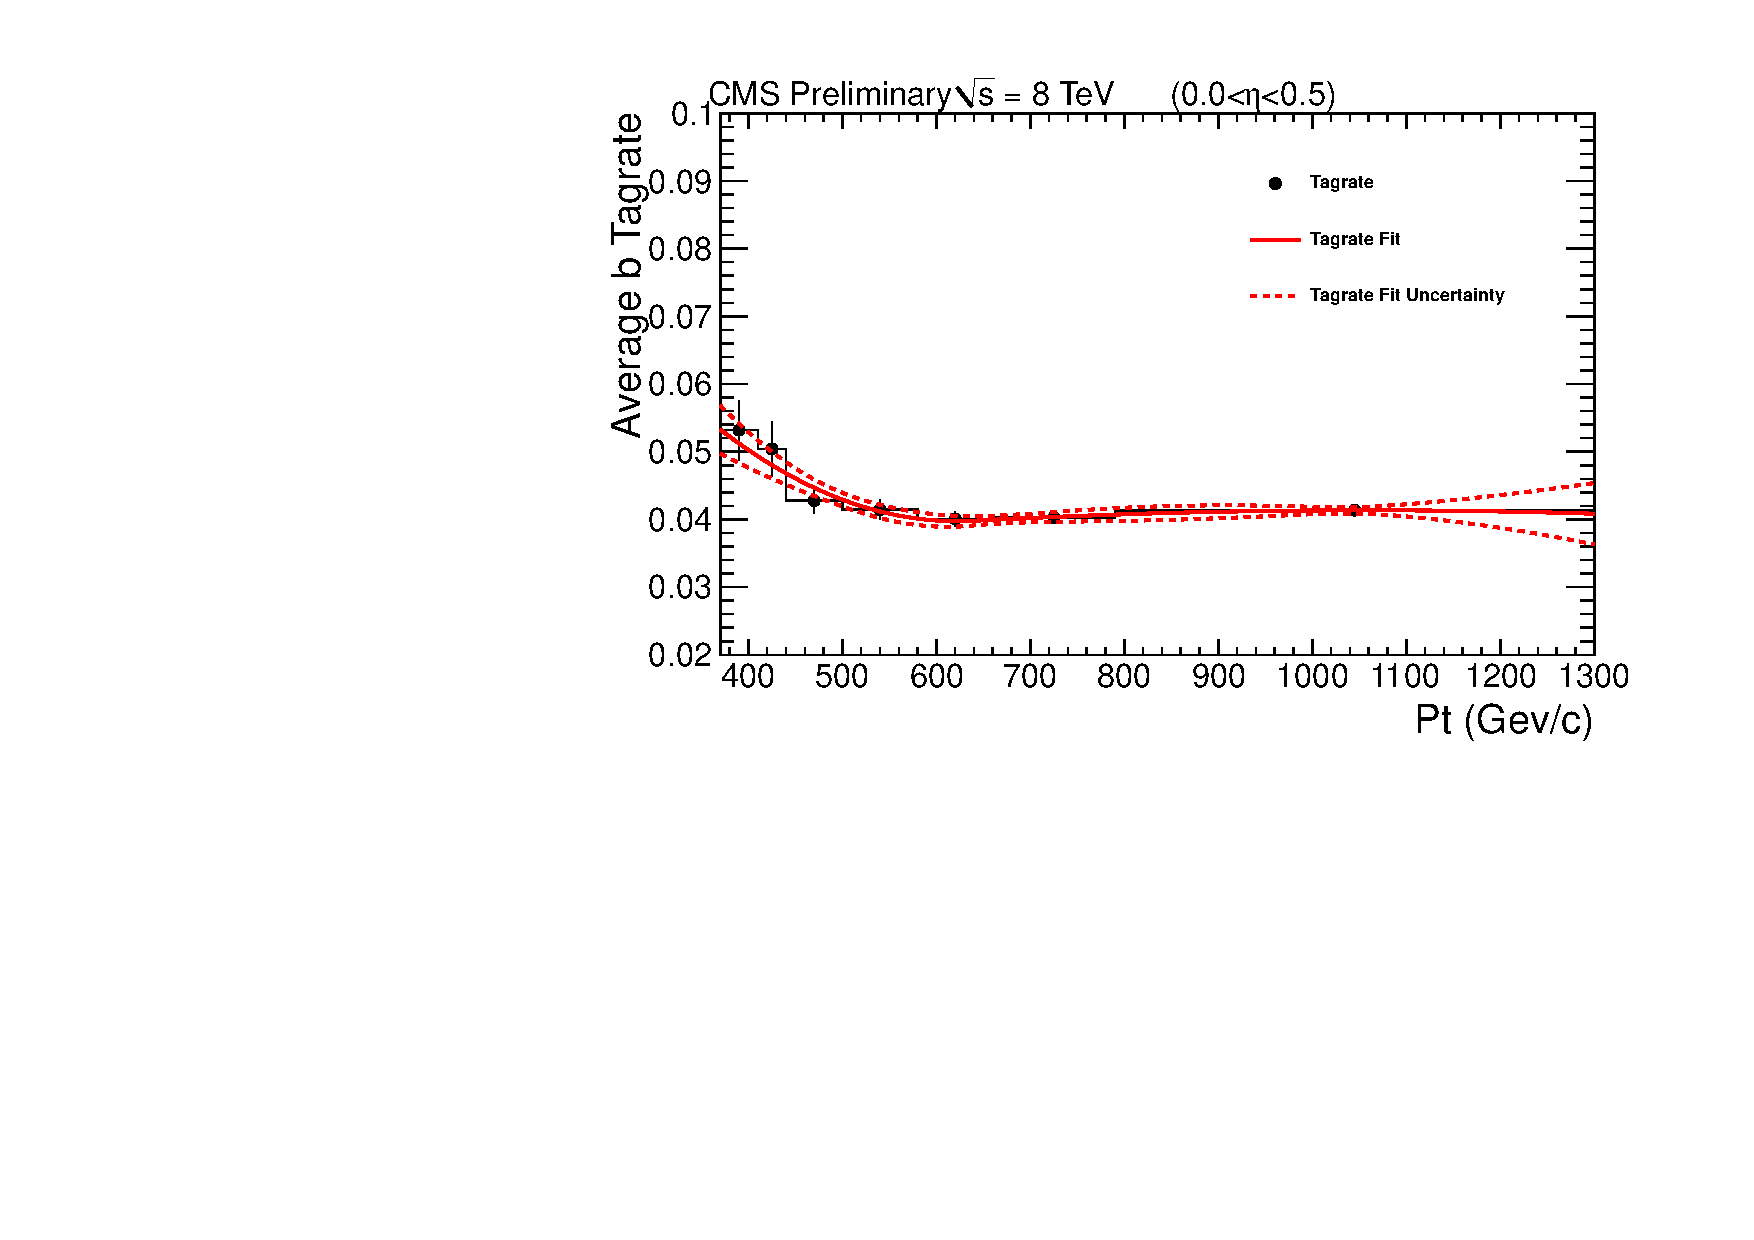
\includegraphics[width=0.75\textwidth]{AN-13-004/figs/tagrateeta1fitBPQCD.pdf}}\\
%\subfigure{\label{figs:tagrateeta2fitBPQCD}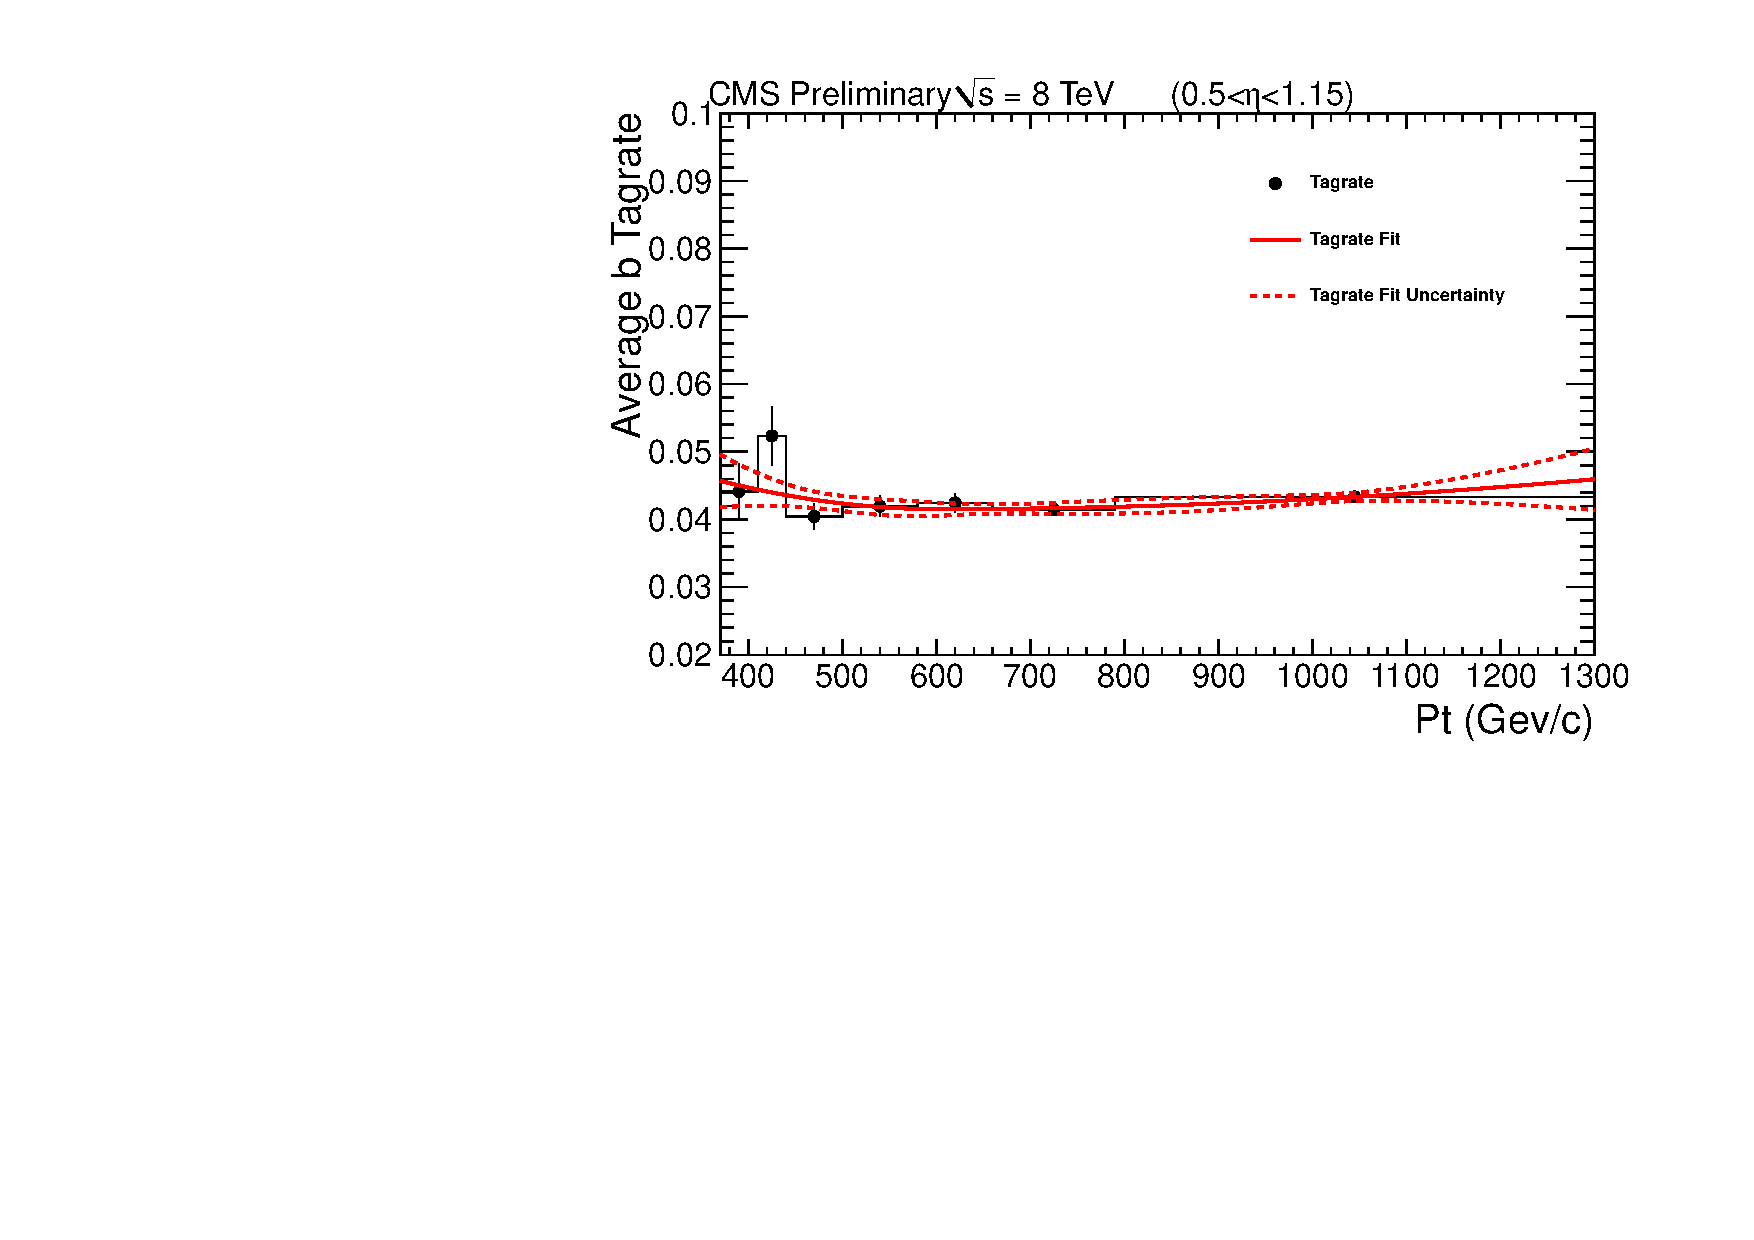
\includegraphics[width=0.75\textwidth]{AN-13-004/figs/tagrateeta2fitBPQCD.pdf}}\\
%\subfigure{\label{figs:tagrateeta3fitBPQCD}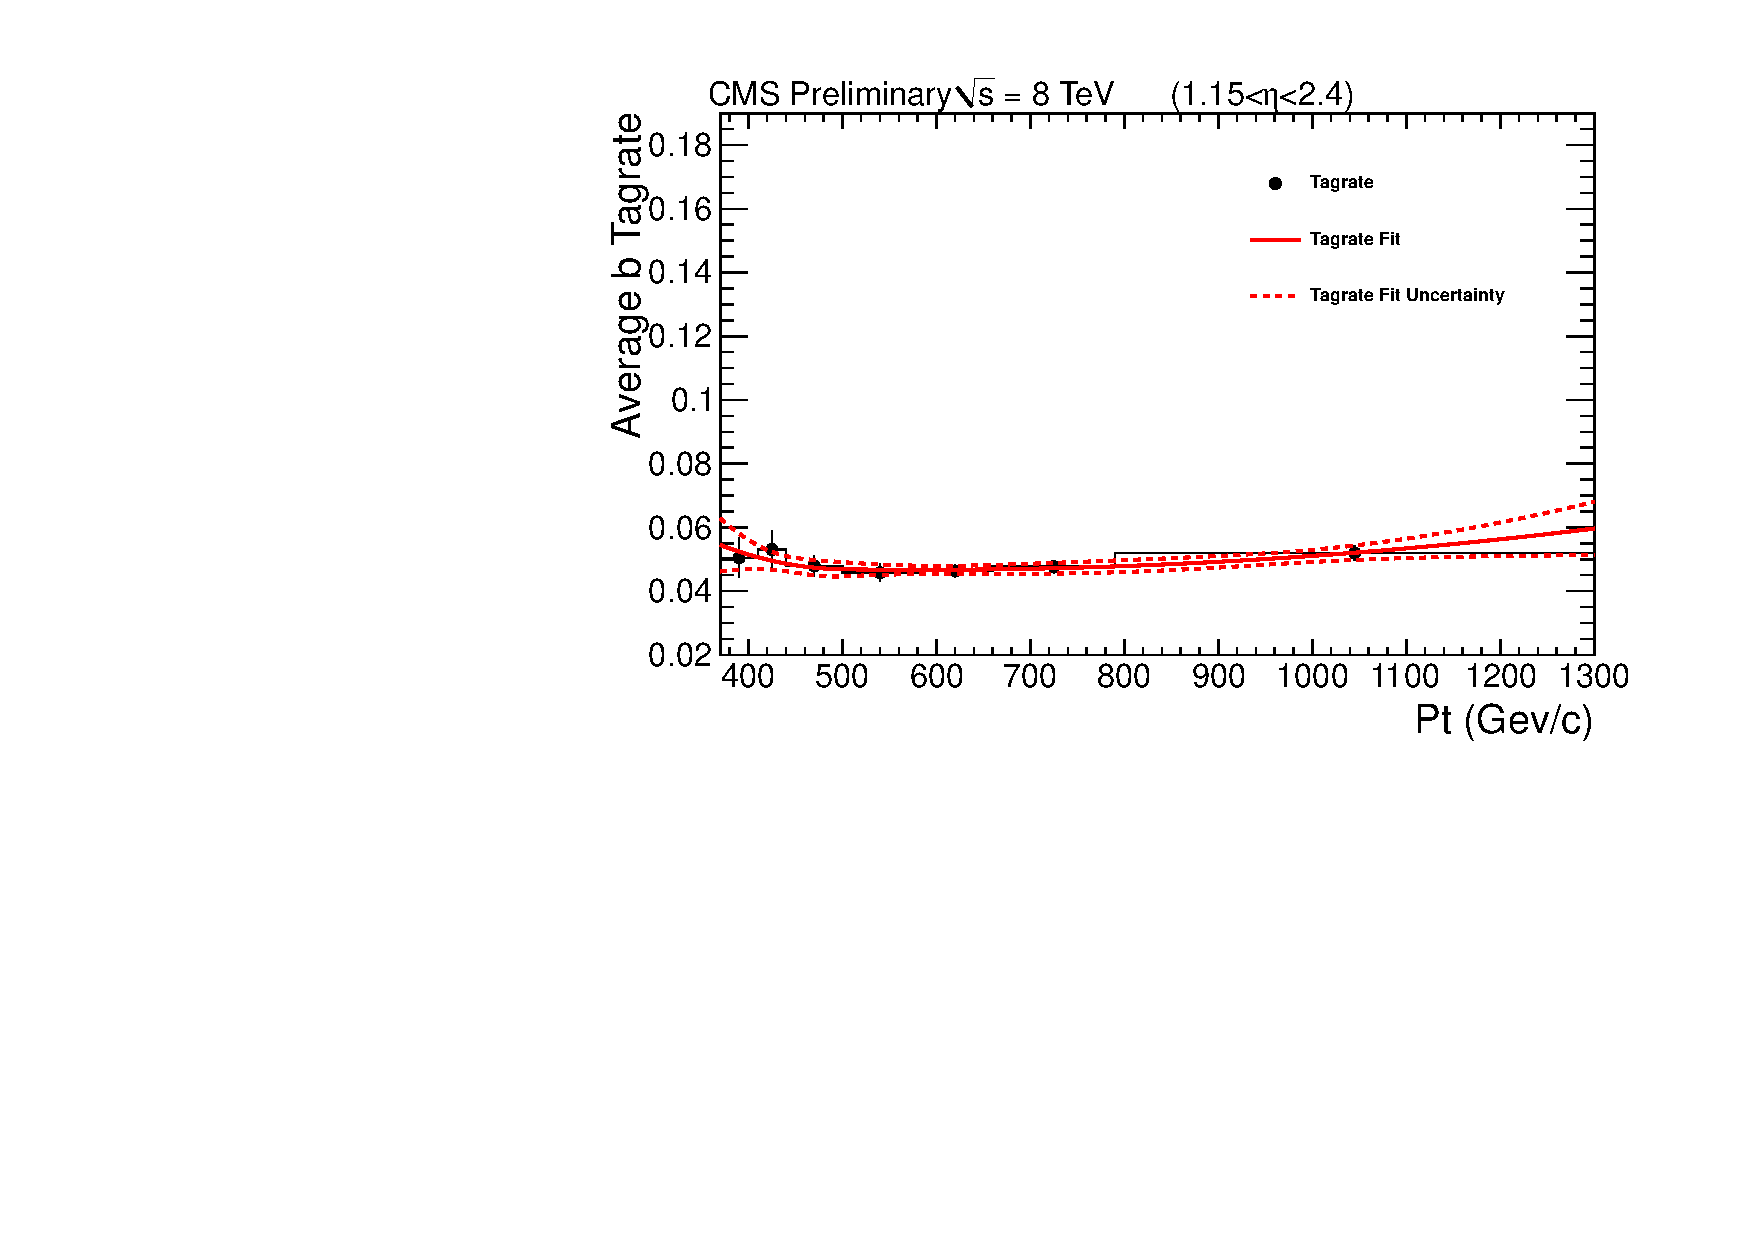
\includegraphics[width=0.75\textwidth]{AN-13-004/figs/tagrateeta3fitBPQCD.pdf}}
%\caption{
%QCD MC $\pt$ parameterized tagrate from
%(a) Low $\eta$ region  
%(b) Transition $\eta$ region 
%(c) High $\eta$ region 
%the average b-tagging rate is shown in black, the polynomial fit is shown in red, and the propagated errors from the fit are shown as a red dashed line.}
%\label{figs:tagrateetafitQCD}
%\end{center}
%\end{figure}

%\begin{figure}[htcb]
%\begin{center}
%\subfigure{\label{figs:tagrateeta1QCD_withSR}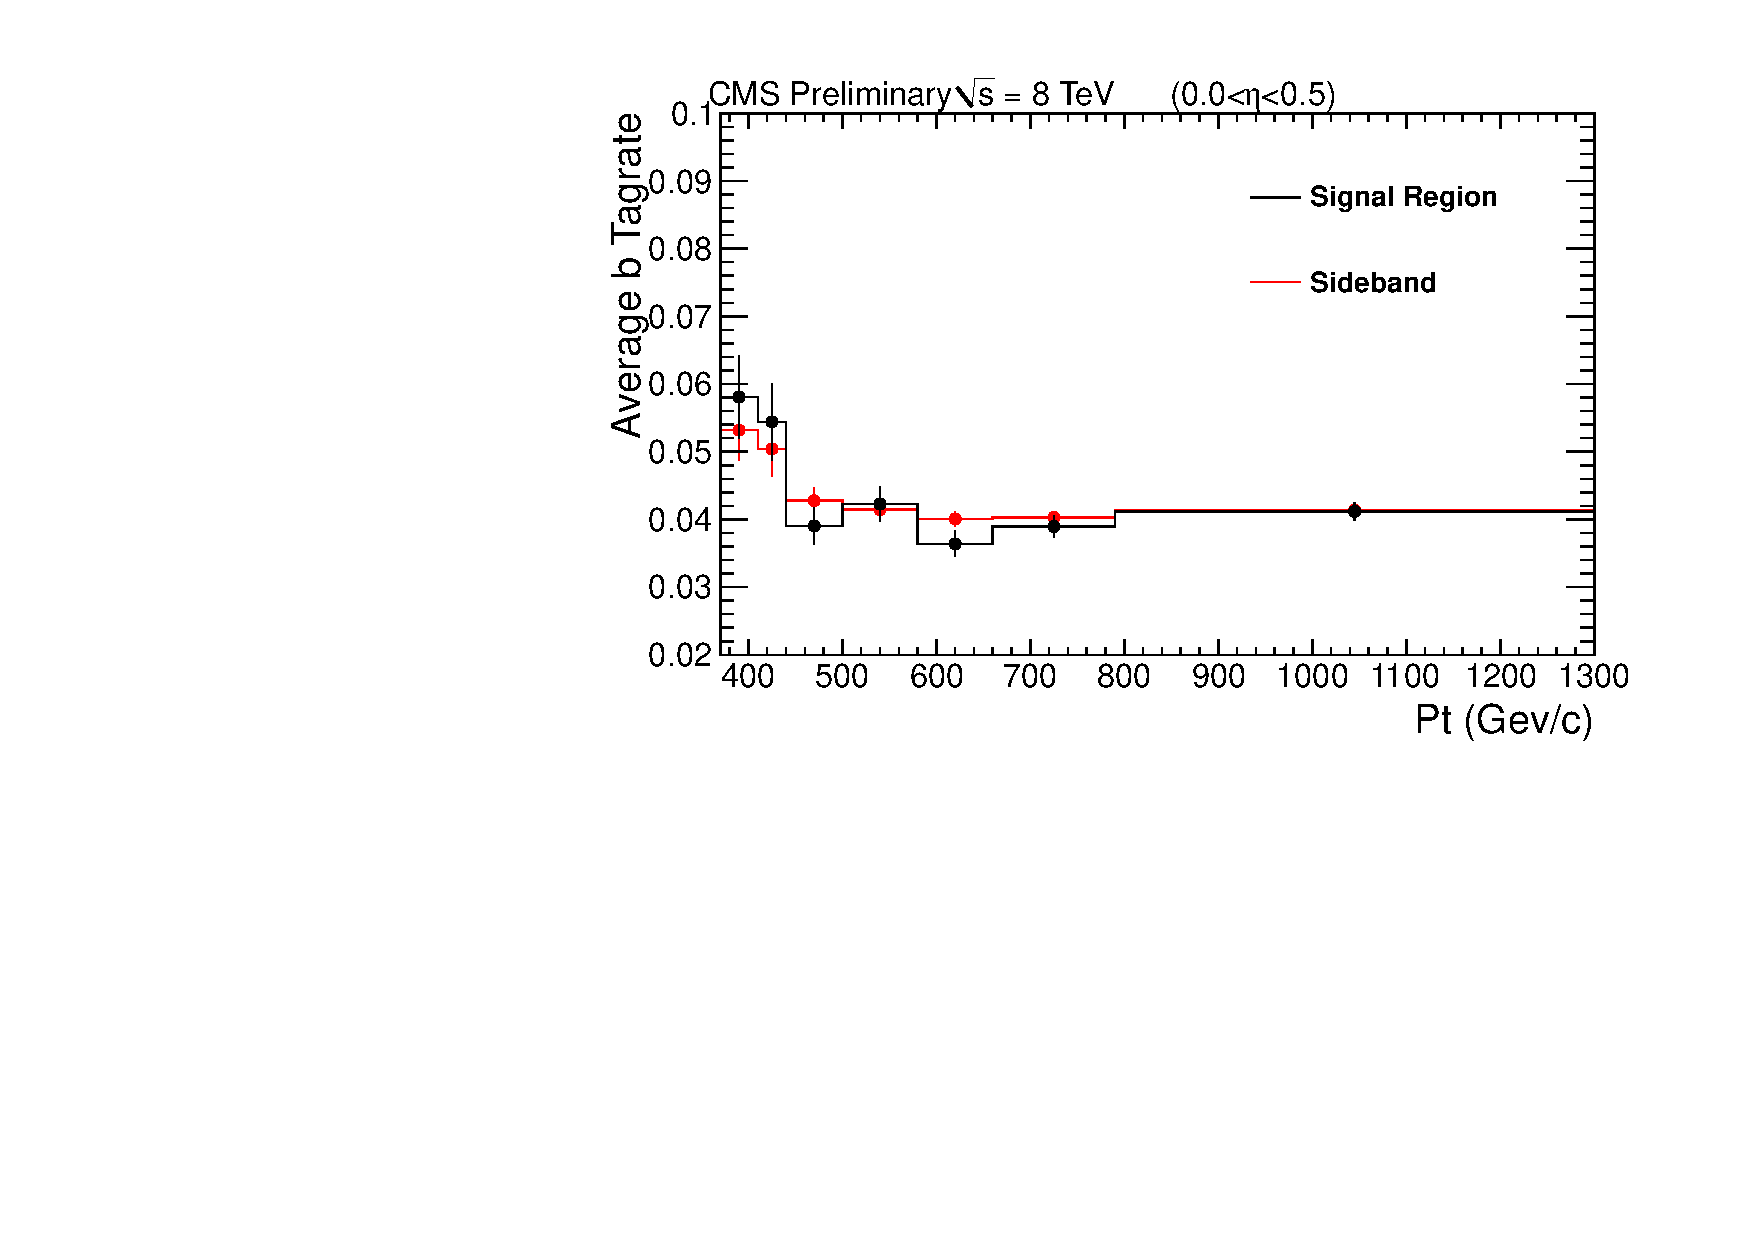
\includegraphics[width=0.75\textwidth]{AN-13-004/figs/tagrateeta1QCD_withSR}}\\
%\subfigure{\label{figs:tagrateeta2QCD_withSR}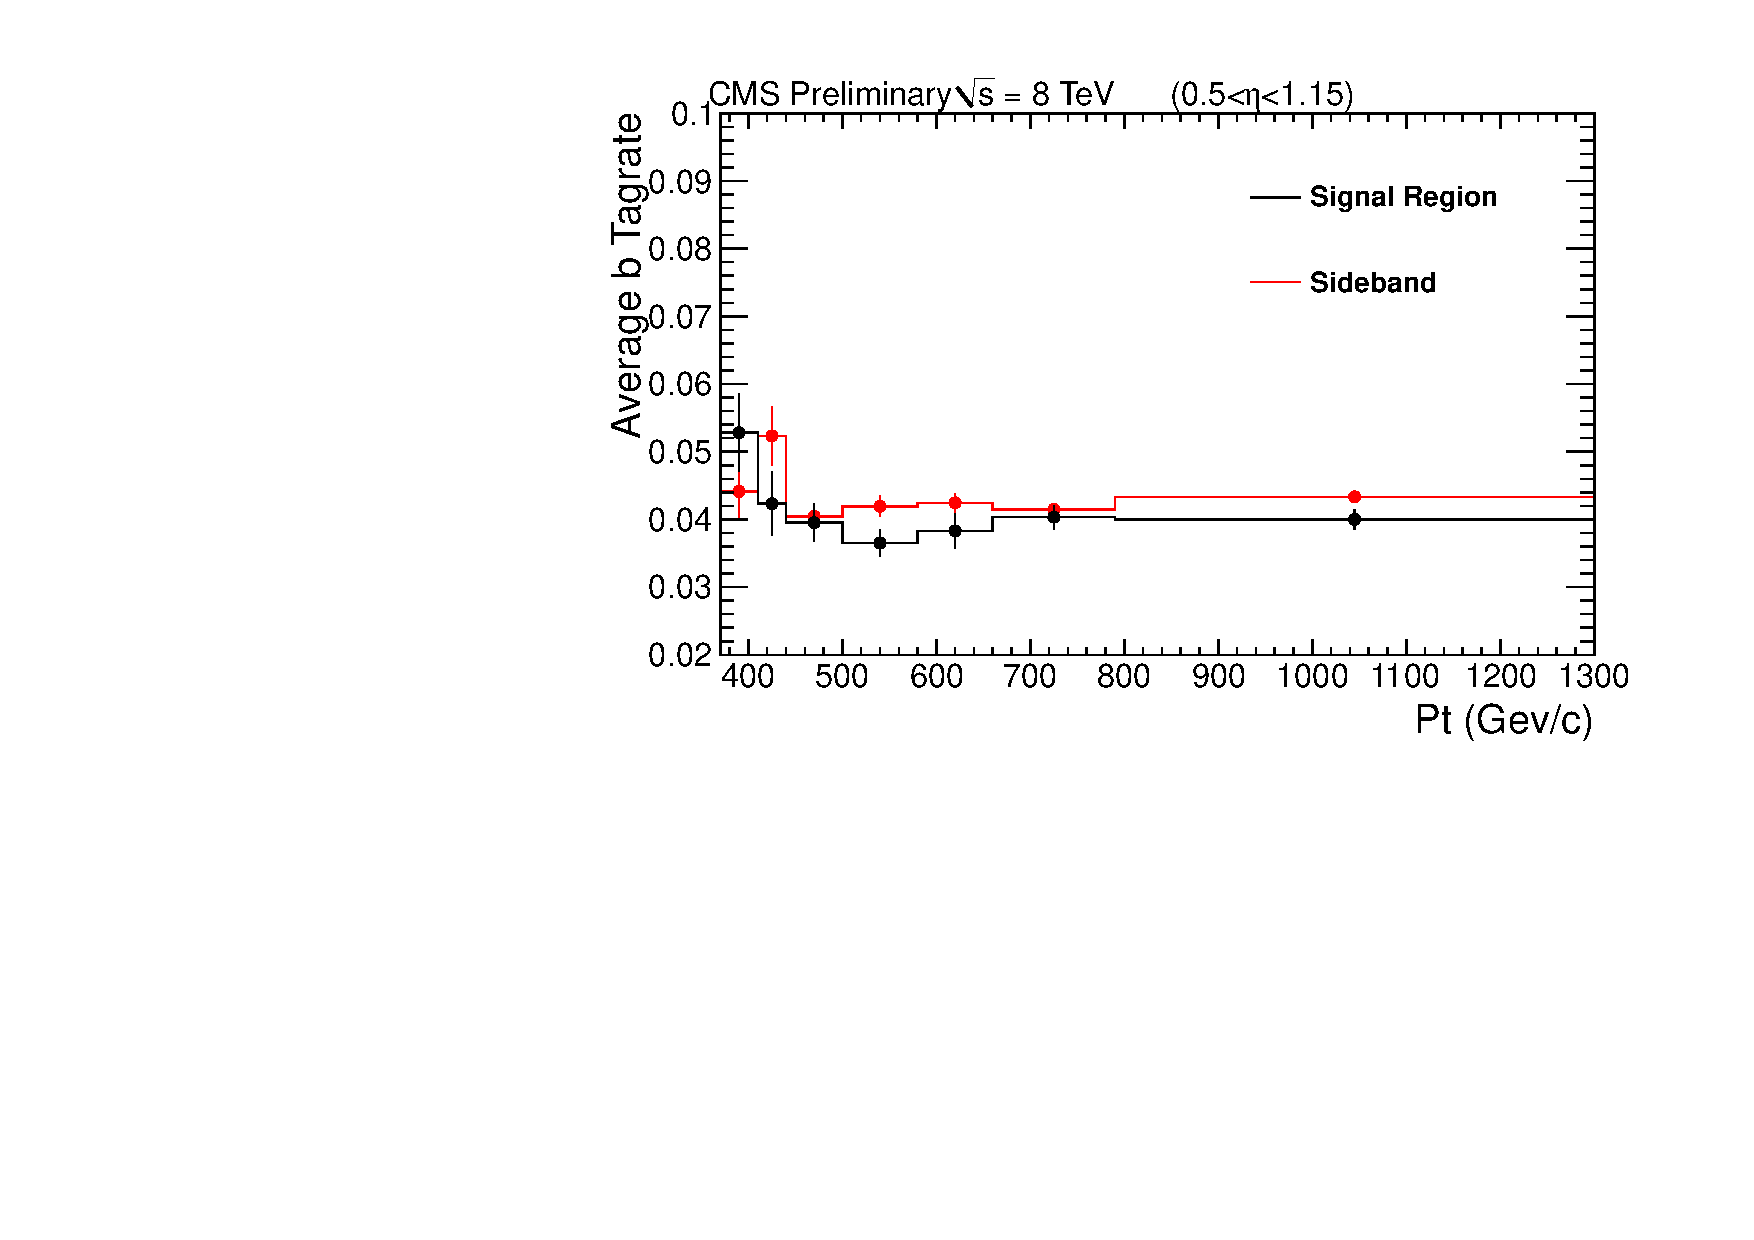
\includegraphics[width=0.75\textwidth]{AN-13-004/figs/tagrateeta2QCD_withSR}}\\
%\subfigure{\label{figs:tagrateeta3QCD_withSR}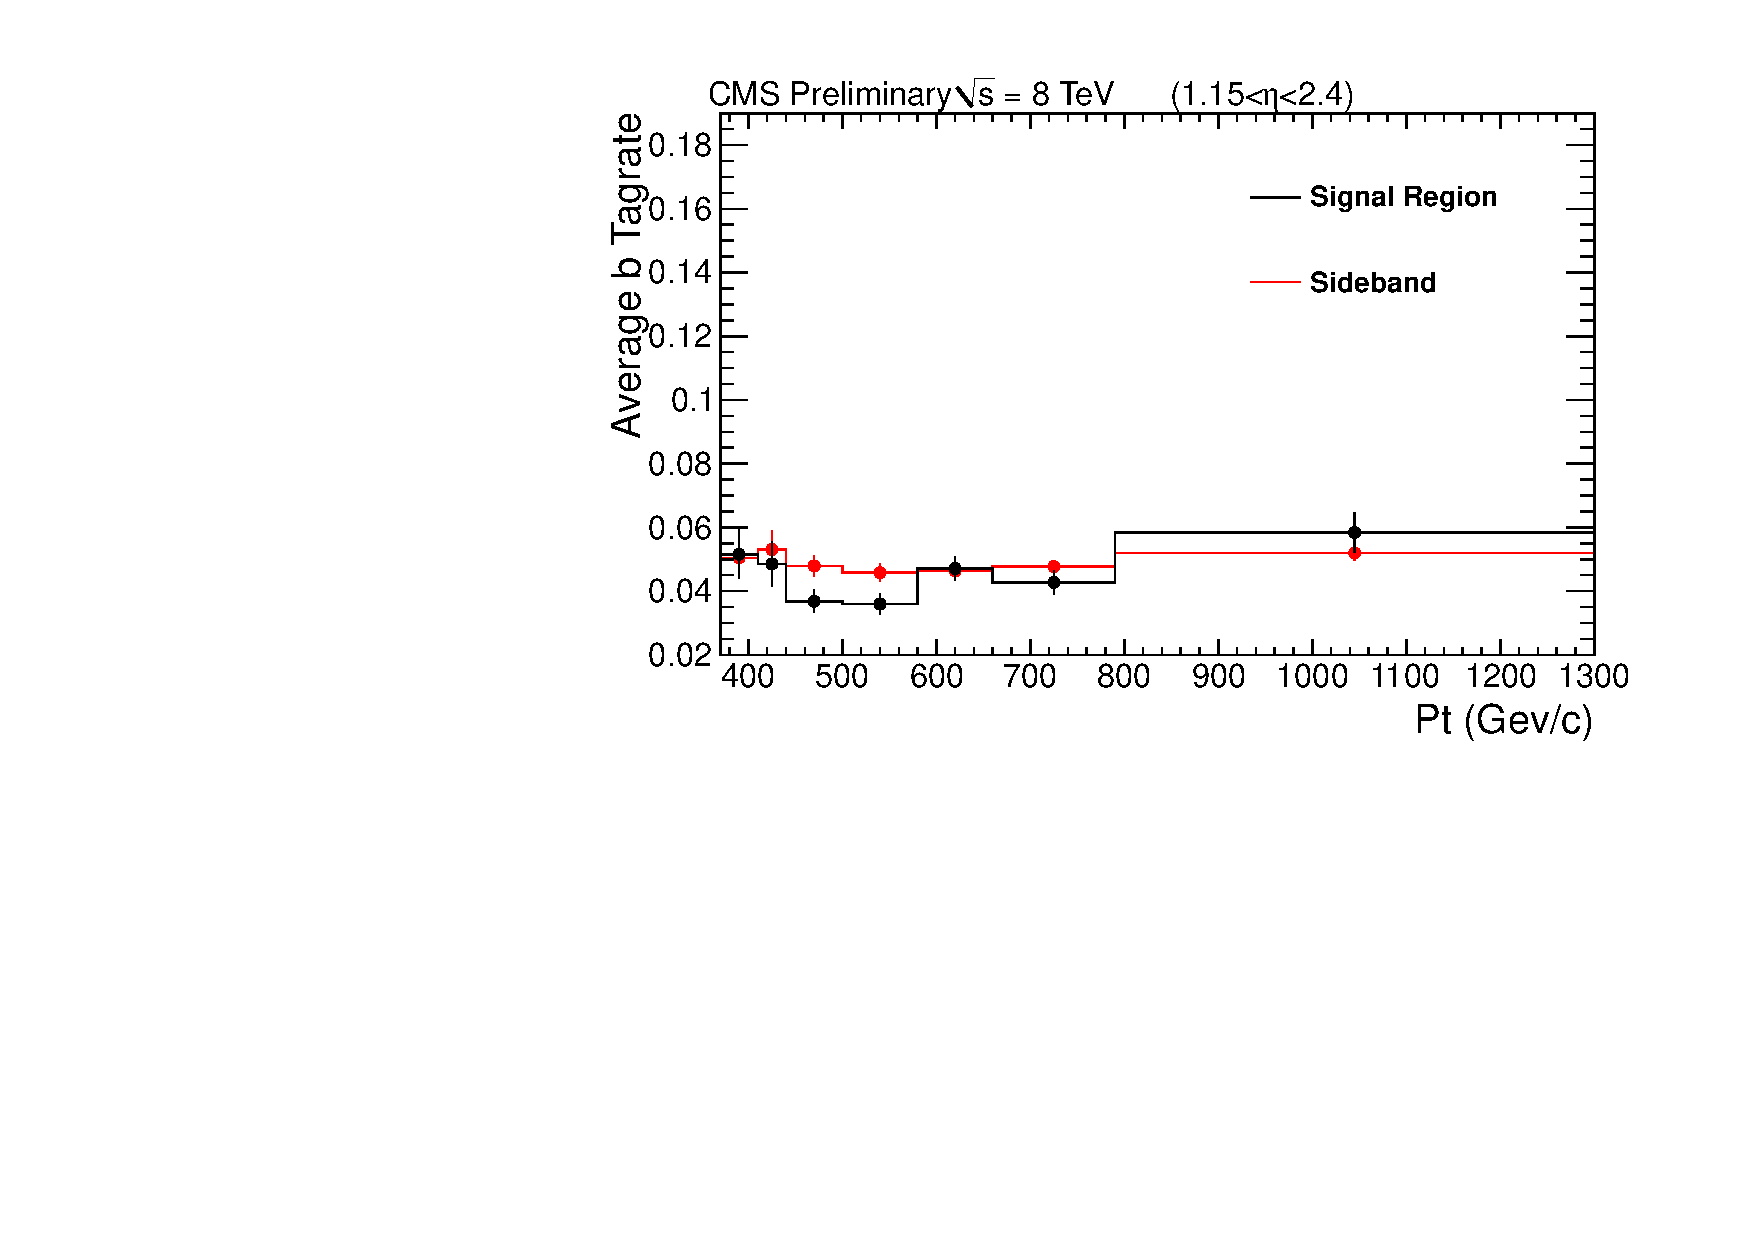
\includegraphics[width=0.75\textwidth]{AN-13-004/figs/tagrateeta3QCD_withSR}}
%\caption{
%QCD MC $\pt$ parameterized tagrate comparison to the signal region from
%(a) Low $\eta$ region  
%(b) Transition $\eta$ region 
%(c) High $\eta$ region 
%the average b-tagging rate from the Signal Region is shown in black, the average b-tagging rate from the Sideband is shown in red.}
%\label{figs:tagrateetaQCD_withSR}
%\end{center}
%\end{figure}

%\begin{figure}[htcb]
%\begin{center}
%\subfigure{\label{figs:MtbvsBkgQCDEO}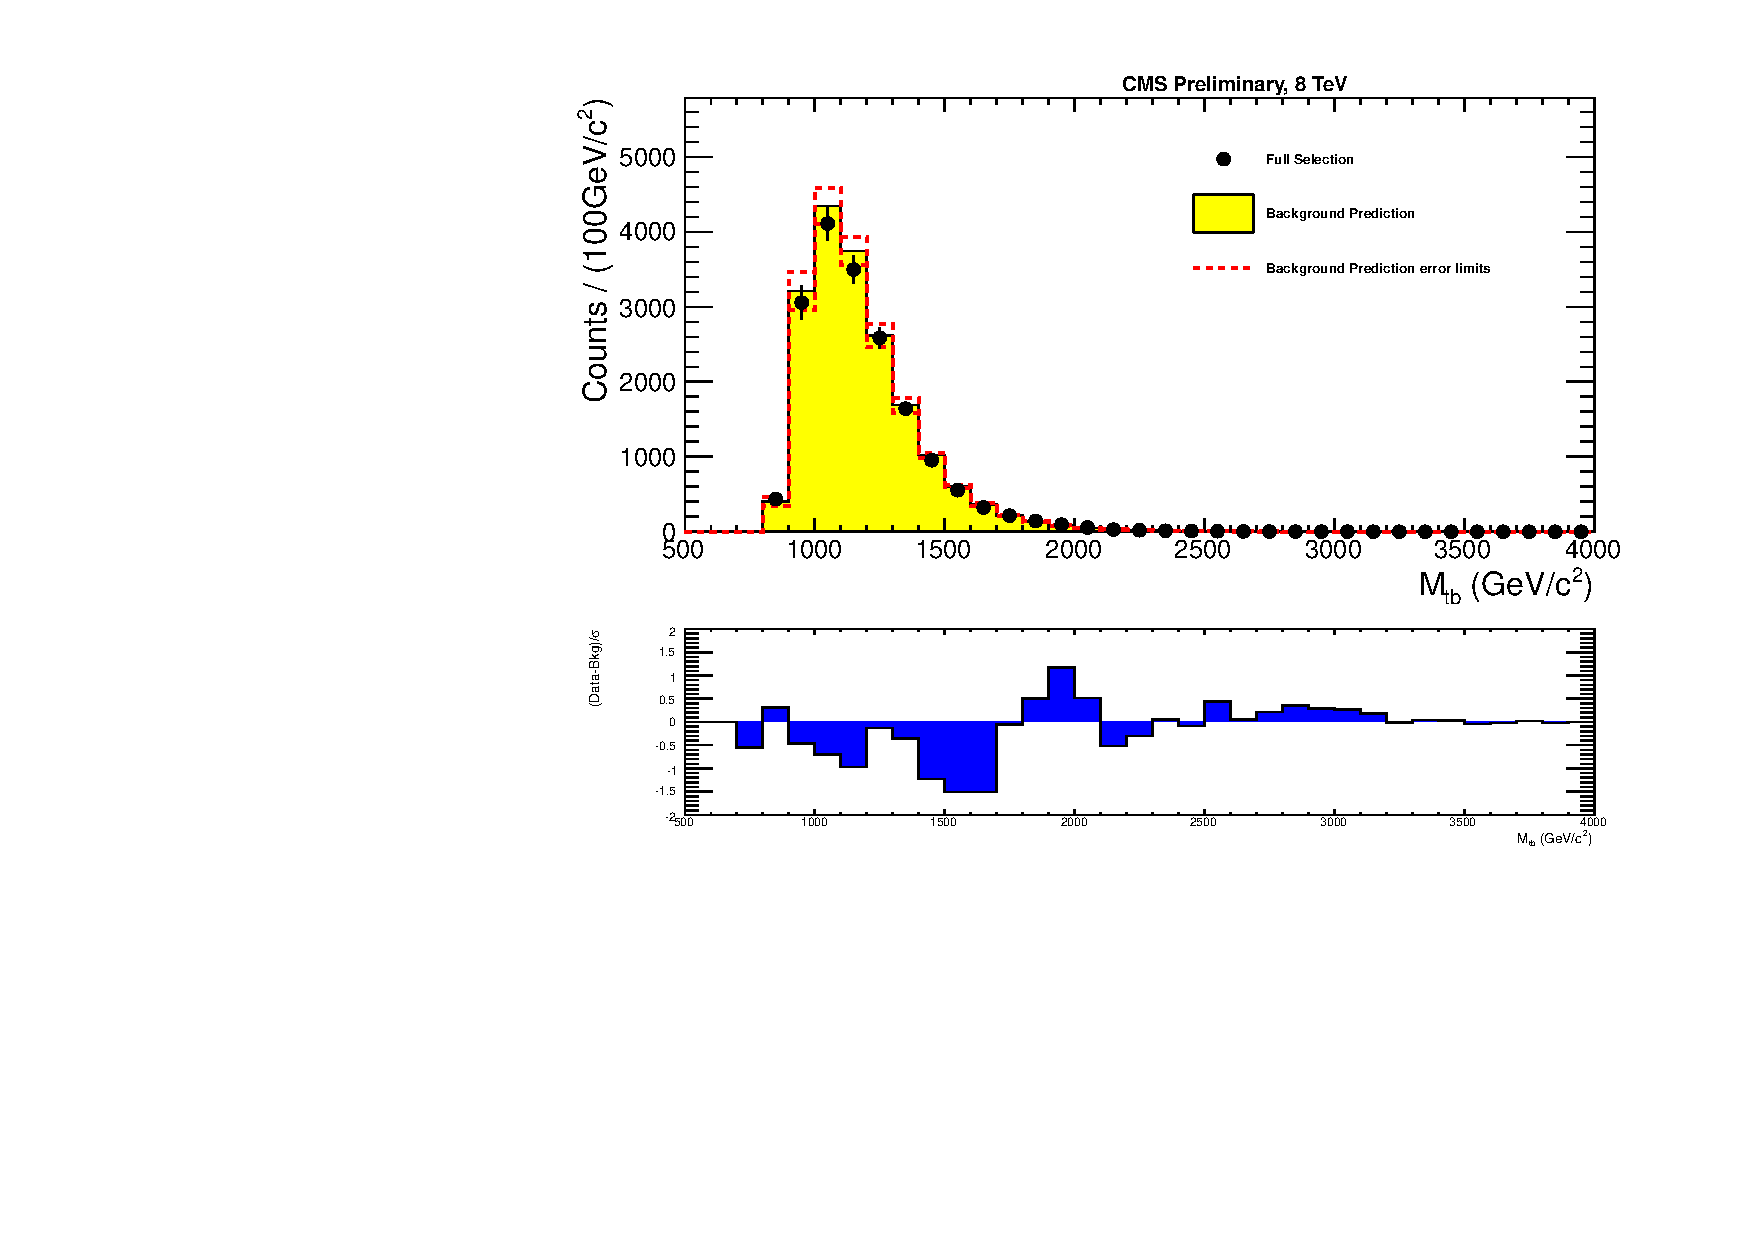
\includegraphics[width=1.0\textwidth]{AN-13-004/figs/MtbvsBkgQCDEO.pdf}}\\
%\subfigure{\label{figs:MtbvsBkgsemilog_QCDEO}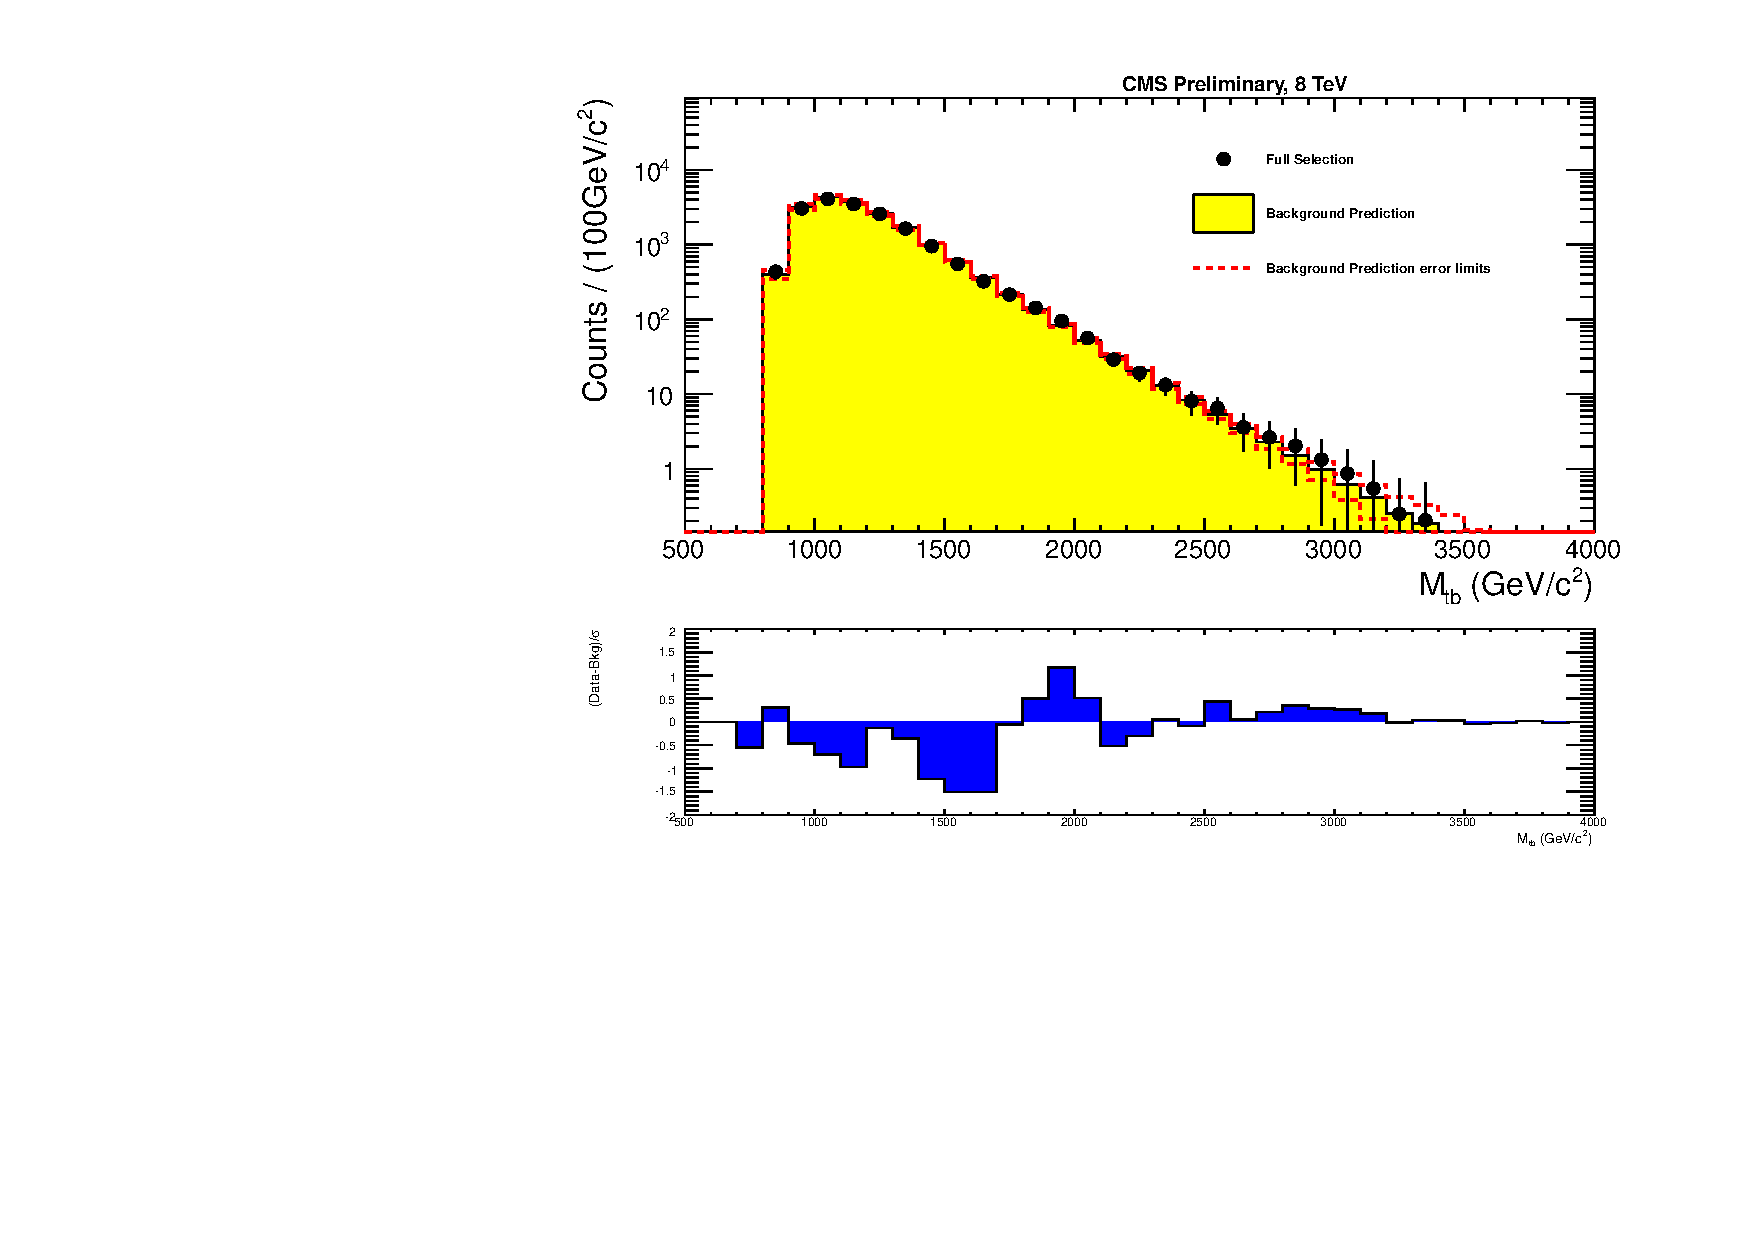
\includegraphics[width=1.0\textwidth]{AN-13-004/figs/MtbvsBkgsemilog_QCDEO.pdf}}
%\caption{
%QCD Monte Carlo background estimation closure test.  The background estimation is extracted from the tagrates shown in Figure\ref{figs:tagrateetafitQCD}.  The full selection is shown in black, 
%the background estimation is shown in yellow, and the errors from the background estimation are shown as a red dashed line.  Top and bottom plots are the same but on linear and log y-axis scale. }
%\label{figs:QCDClosure}
%\end{center}
%\end{figure}

\section{Sideband Closure}
\label{sec:secondsideband}
In order to investigate the applicability and versatility of the QCD background estimation in data, we apply the average b-tagging rate to sideband regions of our top tagging selection.  First, we define the following sideband:

\begin{itemize}
\item {\bf Jet Mass}  $\mathrm{\boldmath 140~\GeV < m_{\text{jet}} < 250~\GeV}$ 
\item {\bf Number of Subjets}  $\mathrm{\boldmath N_{\text{subjets}} > 2}$ 
\item {\bf Minimum Pairwise Mass} $\mathrm{\boldmath m_{\text{min}} \leq 50~\GeV}$ 
\item {\bf N-subjettiness} $\mathrm{\boldmath \tau_3/\tau_2 \geq 0.55}$ 
\item {\bf Subjet b-Tagging} $\mathrm{\boldmath SJ_{\text{CSVMAX}} \geq 0.679}$ 
\end{itemize}
This region lies outside of the signal region and sideband used for average b-tagging rate determination.  
The selection also has a very low yield of $\ttbar$, making it ideal for investigating the QCD background contribution.  
The average b-tagging rate used for this closure test is extracted from the same sideband as the signal region, and applied to pre-b-tagged events.  The closure test can be seen in Figure \ref{figs:NewMtbSB2}.

\begin{figure}[Htcb]
\centering
\subfigure{\label{figs:NewMtbSB21}\includegraphics[width=.9\textwidth]{AN-13-004/figs/NewMtbSB2.pdf}}\\
\subfigure{\label{figs:NewMtbSB22}\includegraphics[width=.9\textwidth]{AN-13-004/figs/NewMtbSB2semilog.pdf}}
\caption{A plot of $M_{tb}$ in the control region defined by inverting the minimum pairwise mass and N-subjettiness cuts used in the full selection.  The top and bottom plots are the same but with linear and log y-axis scale.}
\label{figs:NewMtbSB2}
\end{figure}

Additionally, we can define the following sideband 
\begin{itemize}
\item {\bf Jet Mass}  $\mathrm{\boldmath 140~\GeV < m_{\text{jet}} < 250~\GeV}$ 
\item {\bf Number of Subjets}  $\mathrm{\boldmath N_{\text{subjets}} > 2}$ 
\item {\bf Minimum Pairwise Mass} $\mathrm{\boldmath m_{\text{min}} > 50~\GeV}$ 
\item {\bf N-subjettiness} $\mathrm{\boldmath \tau_3/\tau_2 < 0.55}$ 
\item {\bf Subjet b-Tagging} $\mathrm{\boldmath SJ_{\text{CSVMAX}} \leq 0.679}$ 
\end{itemize}
The closure test can be seen in Figure \ref{figs:NewMtbSB3}.

\begin{figure}[Htcb]
\centering
\subfigure{\label{figs:NewMtbSB31}\includegraphics[width=.9\textwidth]{AN-13-004/figs/NewMtbSB3.pdf}}\\
\subfigure{\label{figs:NewMtbSB32}\includegraphics[width=.9\textwidth]{AN-13-004/figs/NewMtbSB3semilog.pdf}}
\caption{A plot of $M_{tb}$ in the control region defined by inverting the subjet b tagging cut used in the full selection.  The top and bottom plots are the same but with linear and log y-axis scale.}
\label{figs:NewMtbSB3}
\end{figure}

\section{Deriving the normalization of the SM $\ttbar$ production}
\label{sec:ttbarsideband}
In order to study the contribution from $\ttbar$ to tbe full background estimate, we turn to a sideband defined by inverting the b candidate mass requirement in the signal region.
This selection has an amplified $\ttbar$ fraction and is statistically independent from all other sidebands in the analysis.  
This makes the selection ideal for extracting the $\ttbar$ fraction in data.  
In order to extract this fraction, we compare the data-driven QCD background and $\ttbar$ Monte Carlo expectation to the selection in data.  

We perform a template fit to the invariant mass of the b 
candidate, using scaled $\ttbar$ Monte Carlo as one template, and the QCD background prediction as the other.  The fit allows
the QCD background template to move only within its errors, whereas the normalization on $\ttbar$ is unconstrained. 
The optimal parameterization for this fit is in a variable that has distinctly different shapes in $\ttbar$ and QCD.  
We therefore use the b candidate mass, which minimizes the correlation between the QCD and $\ttbar$ templates within the fit. The fit can be seen in Figure \ref{figs:ttbarfit}.  For this maximum likelihood fit we use the Theta package.

Additionally, the fit implements the $\ttbar$ subtraction in the QCD estimate by fitting un-subtracted QCD to the $\ttbar$ full selection.  The output of the fitter is then corrected by  
(1+S/F), where S/F is the ratio of the number of events in $\ttbar$ subtracted selection to the $\ttbar$ full selection. 

This study suggests after all scale factors applied in the analysis, the $\ttbar$ contribution needs to be amplified by $1.23 \pm 0.24$.  
This normalization is used for all $\ttbar$ distributions in the analysis, and the uncertainty is then the full normalization uncertainty for $\ttbar$.

\begin{figure}[htcb]
\centering
\includegraphics[width=1.0\textwidth]{AN-13-004/figs/ttbarfittingfromthetatmass}
\caption{b candidate mass as extracted from the b candidate mass inverted sideband.  Pre fraction fit (left) and post fraction fit (right).}
\label{figs:ttbarfit}
\end{figure}





\chapter{Data Results}
After closure of the background estimation procedure within the control region \ref{sec:bssecondsideband}, we investigate signal region.  
The results in the signal region are shown in Figure \ref{figs:bsMtwvsBkg1}.  We proceed to compute 
limits on the $\bs$ cross-section.  Background estimation of selected relevant variables can be seen in 
Figures \ref{figs:bskinplotsdata1} and \ref{figs:bskinplotsdata2}.

The expected number of events in the signal region is 359 $\pm$ 58, the observed number of events is 318.  Table \ref{table:bssigeff} gives the signal efficiency in the signal region for 
the three signal coupling hypotheses.

\begin{table}
\begin{center}
\bf{$\bs$ signal region efficiency}\\
\begin{tabular}{|c||c|c|c|}
\hline
\bf{$\mathrm{M_{\bs}}$} & \bf{$\epsilon_{R}$}  & \bf{$\epsilon_{L}$} & \bf{$\epsilon_{LR}$} \\
\hline
800 & 0.0014 & 0.0010 & 0.0012\\
\hline
900 & 0.0076 & 0.0063 & 0.0070\\
\hline
1000 & 0.0301 & 0.0243 & 0.0272\\
\hline
1100 & 0.0502 & 0.0411 & 0.0456\\
\hline
1200 & 0.0653 & 0.0522 & 0.0588\\
\hline
1300 & 0.0746 & 0.0590 & 0.0668\\
\hline
1400 & 0.0788 & 0.0636 & 0.0712\\
\hline
1500 & 0.0809 & 0.0629 & 0.0719\\
\hline
1600 & 0.0795 & 0.0616 & 0.0706\\
\hline
1700 & 0.0760 & 0.0596 & 0.0678\\
\hline
1800 & 0.0749 & 0.0569 & 0.0659\\
\hline
1900 & 0.0707 & 0.0536 & 0.0622\\
\hline
2000 & 0.0660 & 0.0499 & 0.0583\\
\hline
\end{tabular}
\end{center}
\caption{$\bs$ signal efficiency for left-handed, right-handed and vectorlike $\bs$ samples}
\label{table:bssigeff}
\end{table}





\begin{figure}[htcb]
\begin{center}
\subfigure{\label{figs:bsMtwvsBkg_BifPoly_fit}\includegraphics[width=0.7\textwidth]{AN-14-049/figs/MtwvsBkg_BifPoly_fit.pdf}}\\
\subfigure{\label{figs:bsMtwvsBkgsemilog_BifPoly_fit}\includegraphics[width=0.7\textwidth]{AN-14-049/figs/MtwvsBkgsemilog_BifPoly_fit.pdf}}
\caption{
A plot of the full selection comparing data, signal and background.  
Top and bottom plots are the same but on linear and log y-axis scale.}
\label{figs:bsMtwvsBkg1}
\end{center}
\end{figure}

\begin{figure}[htcb]
\centering
\includegraphics[width=.7\textwidth]{AN-14-049/figs/KinPlots_Data1.pdf}
\caption{Background estimation of kinematic variables.  
The error bars shown are from the three primary sources; uncertainty on the fit, choice of fit, top mass modification, $\ttbar$ normalization, and $\ttbar$ $Q^2$ uncertainty}
\label{figs:bskinplotsdata1}
\end{figure}  
\clearpage

\begin{figure}[htcb]
\centering
\includegraphics[width=.7\textwidth]{AN-14-049/figs/KinPlots_Data2.pdf}
\caption{Background estimation of kinematic variables.  
The error bars shown are from the three primary sources; uncertainty on the fit, choice of fit, top mass modification, $\ttbar$ normalization, and $\ttbar$ $Q^2$ uncertainty}
\label{figs:bskinplotsdata2}
\end{figure}  
\clearpage


\clearpage
\newpage
\section{Systematic Uncertainties}
\label{sec:systematics}
Various systematics are taken into account, both 
on our expected signal and background estimate. Some systematic uncertainties will affect only the normalization of certain event rates, 
and are reported as overall normalization uncertainties. Other systematics affect the shapes of the reconstructed signal or backgrounds, as well as their normalization.  The
Systematic uncertainties that are used in the analysis are summarized in table \ref{table:nuisance}.% All systematic effects are listed in Table \ref{table:systeffects}.

%\begin{sidewaystable}
%\begin{center}
%\begin{small}
%\begin{tabular}{| c || c || c | c | c  c  c  c  c  c  c  c |}
%\hline
%& \textbf{Process:} & $t\overline{t}$ & QCD & & & & & & & &\\
%& \textbf{$W^\prime$ Mass Point:} & & & 1300 & 1500 & 1700 & 1900 & 2100 & 2300 & 2700 & 3100  \\
%\hline
%\textbf{Systematic} & \textbf{Variation ($\%$)} & \multicolumn{9}{c}{\textbf{Effect of Systematic} (\%)} \\ 
%\hline
%Luminosity & $\pm 4.4$ & 4.4 &  & 4.4 & 4.4 & 4.4 & 4.4 & 4.4 & 4.4 & 4.4 & 4.4 \\
%Subjet Scale Factor & $\pm 5$ & 5 &  & 5 & 5 & 5 & 5 & 5 & 5 & 5 & 5 \\
%$t\overline{t}$ cross-section & $\pm 50$ & 50 & & & & & & & & & \\
%b-tagging & see text & 7 & & 8 & 8 & 9 & 9 & 11 & 11 & 12 & 10  \\
%Trigger Efficiency & see text & 7 & & 1 & $<1$ & $<1$ & $<1$ & $<$1 & $<1$ & $<1$ & $<1$  \\
%Jet Energy Scale$^{up}_{down}$ & $\pm 5$ & $^{22}_{20}$ & & $^{7}_{11}$ & $^{1}_{4}$ & $^{1}_{2}$ & $^{12}_{0.1}$ & $^{4}_{1}$ & $^{4}_{1}$ & $^{4}_{1}$ & $^{0.5}_{3}$  \\
%QCD Systematic & see text & & 4 & & & & & & & &  \\
%\hline
%Number of Events& & 1042 & 17901 & 579 & 274 & 118 & 51 & 22 & 10 & 2 & 1 \\
%\hline
%\end{tabular}
%\caption{Effect of systematics listed in Section \ref{sec:systematics}, computed over the entire mass-range.  The b-tagging, Jet Energy Scale, and Trigger uncertainties have non negligible 
%shape based effects that must be taken into account. Note: the $2\%$ b-tagging systematic derived in Section \ref{sec:btagging} is included in the b-tagging line above.}
%\label{table:systeffects}
%\end{small}
%\end{center}
%\end{sidewaystable}

\subsection{Jet Energy Scale}
We evaluate the effect of uncertainty on the jet energy scale on samples derived from MC simulation.  
To do so, we vary the jet four-momentum up and down by the jet energy 
scale uncertainty, which we take to be $3\%$. We include $\pt$ and $\eta$ dependent corrections to the 
jet energies, as well as uncertainties from the difference in measured and simulated $W$ masses \cite{ZP8TeV}. 

Varying the jet momentum can cause a jet to fall below or rise above the $\pt$ cut in the analysis, thus shifting the invariant 
mass spectrum of the signal and reconstructed $\ttbar$ samples. Figure \ref{figs:ttbarJES} shows the systematic shapes from the 
jet energy scale on the $\ttbar$ distribution.  Jet Energy scale variation on signal MC is shown in Figure \ref{figs:signalJES} for 1300$~\GeV$,
 1900$~\GeV$, and 2300$~\GeV$ mass points.

\subsection{Trigger}
We include an uncertainty based on the measured trigger efficiency for all MC Samples. The trigger efficiency is discussed in Section \ref{sec:trigger}. 
To obtain shape systematics from this effect, we vary the trigger by half the trigger \textit{in}efficiency. The effects of this on the $t\overline{t}$ 
distribution is shown in Figure \ref{figs:ttbartrig}. Trigger weighting on signal MC is shown in Figure \ref{figs:signaltrig} for 1300$~\GeV$,
 1900$~\GeV$, and 2300$~\GeV$ mass points.  The uncertainty is low in the mass range of interest for limit setting.

\subsection{Jet Energy Resolution}
\label{sec:JER}
We apply a systematic due to the known differences in jet energy resolution in data and simulation.  We use $\eta$ dependent smearing (see \cite{ZP8TeV}) as recommended by the JER group.  
We apply this systematic uncertainty to the $t\overline{t}$ distribution 
(as seen in Figure \ref{figs:ttbarJER}).  Jet Energy Resolution variation on signal MC is shown in Figure \ref{figs:signalJER} for 1300$~\GeV$,
 1900$~\GeV$, and 2300$~\GeV$ mass points. 

\subsection{Jet Angular Resolution}
A smearing of $10\%$ is assumed on $\eta$ and $\phi$ and shape uncertainties are generated by considering smearing $10\%$ 
lower and higher. We apply this systematic uncertainty to the $\ttbar$ distribution (as seen in Figure \ref{figs:ttbarJAR} ). Jet Angular Resolution 
variation on signal MC is shown in Figure \ref{figs:signalJAR} for 1300$~\GeV$,
 1900$~\GeV$, and 2300$~\GeV$ mass points.  The effect is very small and thus not considered in setting limits.

\subsection{PDF Uncertainty}
The uncertainty in the parton distribution function used for MC sample generation is investigated.  We take the average of the $\pm$1$\sigma$ eigenvalue 
variation of the pdf master equations \cite{Bourilkov:2006cj} 
for the NNPDF, MSTW2008nnlo, and CT10 pdf sets to weight the signal and $\ttbar$ MC samples and investigate the impact on the full selection.  The PDF set 
that provides the maximum uncertainty is then used for the $\pm$1$\sigma$ PDF uncertainty.  For $\ttbar$ and signal this set is NNPDF. PDF 
variation on signal MC is shown in Figure \ref{figs:signalPDF} for 1300$~\GeV$,
 1900$~\GeV$, and 2300$~\GeV$ mass points.  PDF variation on $\ttbar$ MC is shown in Figure \ref{figs:ttbarPDF}.  The effect is very small and thus not considered in setting limits.

\subsection{Pileup}
A study of pileup uncertainty is conducted by varying the minimum bias cross-section by 5\% as a measure of systematic uncertainty.  The results 
can be seen in figure \ref{figs:signalPU}.  The effect is very small and thus not considered in setting limits.

\subsection{b-Tagging Scale Factor Uncertainty}
\label{sec:btagunc}
The uncertainty in the b-tagging scale factor described in Section \ref{sec:btagging} is applied based on the b candidate pt.  The binning and associated errors 
listed below are the suggested EPS13 prescription generated from measurements in both muon-jet and ttbar data representing 20$~\fbinv$ of integrated 
luminosity.  The absolute uncertainty on $\mathrm{SF_b}$ for a b candidate jet within the listed $\pt$ range is applied as shown in table \ref{table:btaggingerrors} 
for $\pt < 800~\GeV$.  B candidate jets with $\pt > 800~\GeV$ are assigned an uncertainty equal to twice the listed value for $600~\GeV < \pt < 800~\GeV$

\begin{table}
\begin{center}
\begin{tabular}{l|c} 
\hline\hline
\bf{$\pt$ range } & \bf{Absolute Error on $\mathrm{SF_b}$} \\
\hline\hline
$320~\GeV < \pt < 400~\GeV$ & 0.0313175 \\
$400~\GeV < \pt < 500~\GeV$ & 0.0415417 \\
$500~\GeV < \pt < 600~\GeV$ & 0.0740446 \\
$600~\GeV < \pt < 800~\GeV$ & 0.0596716 \\
\hline
\end{tabular}
\end{center}
\caption{Absolute Error applied to the b-tagging Scale Factor}
\label{table:btaggingerrors}
\end{table}


%\clearpage

\subsection{$\mathrm{Q^2}$ Scale Uncertainty}
We use additional $\ttbar$ samples generated with twice and half the nominal $\mathrm{Q^2}$ 
scale used in the $\ttbar$ samples listed in table \ref{table:datasets}.  These samples vary the renormalization and factorization scales to account for 
missing higher order corrections in our simulation.  Figure \ref{figs:q2scale} shows the shape based uncertainty due to this effect.

\begin{figure}[htcb]
\begin{center}
\includegraphics[width=0.7\textwidth]{AN-13-004/figs/TTbar_Q2Scale}
\caption{
$\mathrm{Q^2}$ systematic variation for $\ttbar$ MC 
}
\label{figs:q2scale}
\end{center}
\end{figure}

\subsection{$\ttbar$ $\pt$ Re-weighting}
The uncertainty related to the $\pt$ re-weighting scheme presented in Section \ref{sec:ttptrw} is taken as the difference between the weighted and unweighted $\ttbar$ spectrum.
%However, this scheme has both a normalization and shape based effect.  Due to the fact that we extract the $\ttbar$ normalization uncertainty (see Section \ref{sec:ttbarsideband}), 
%we normalize the up and down systematic to the nominal $\pt$ re-weighting and use this in limit setting.
This uncertainty can be seen in figure \ref{figs:ptreweight}.  This is the dominant uncertainty for $\ttbar$. 

\begin{figure}[htcb]
\begin{center}
\includegraphics[width=0.7\textwidth]{AN-13-004/figs/TTbar_PTReweighting}
\caption{
$\pt$ re-weighting systematic variation for $\ttbar$ MC 
}
\label{figs:ptreweight}
\end{center}
\end{figure}

\subsection{Normalization Uncertainties}
As mentioned in Section \ref{sec:ttbarsideband}, the uncertainty due to the overall normalization scale factor used for $\ttbar$ is extracted from data and is $19\%$.   

We must apply a $13\%$ uncertainty on the top tagging scale factor described in Section \ref{sec:subjetSF} to signal MC events due to uncertainty in the difference in subjet efficiency from data to MC.

As mentioned in Section \ref{sec:btagging}, we add a $2\%$ uncertainty to the signal estimates from the AK5 vs. CA8 scale factor on b-tagging efficiency. 

We also include a $2.6\%$ uncertainty in the luminosity for the signal MC \cite{CMS-PAS-LUM-13-001}. 


\clearpage
\subsection{Uncertainties related to the QCD Background Estimate}
We use the result of the fit to the average b-tagging rate (see Section \ref{sec:backgroundEstimation}) to weight 
pre b-tagged events in order to create the QCD background estimate.  Uncertainties in
the fitting algorithm and statistical uncertainties in the sideband
are taken into account (see figure \ref{figs:tagrateetafit}).
Statistical uncertainties in the pre b tagged signal region are also
taken into account.

\subsubsection{Choice of the functional form for the average b-tagging rate}
\label{sec:choiceoffit}
The functional form used is a bifurcated polynomial.
However there is a systematic uncertainty associated with this choice.
The uncertainties due to this effect are taken into account by
studying alternative functional forms seen in figure
\ref{figs:BKGFITCOMP}.  The background estimation from these
alternative fits are seen in figure \ref{figs:BKGCOMP}.  The
uncertainty due to the choice of fit is taken as the Mean Squared
Error of these alternative backgrounds bin by bin and can be seen in
figure \ref{figs:BKGERR}.  


\subsubsection{Two-dimensional  vs. three-dimensional parameterization of the average b-tagging rate}
\label{sec:paramerrors1}
Additionally, we place an uncertainty on the inability of the
background estimate to capture all kinematic correlations through the
parameterization of the average b-tagging rate in $\pt$ and $\eta$.
This uncertainty is calculated by investigating a parameterization in
$\pt$ $\eta$ and $\mathrm{M_{tb}}$.  We define $P_i$ as the average b-tagging
rate described in Section \ref{sec:backgroundEstimation} in one
$\eta$ bin and $P_{ij}$ as the average b-tagging rate if parameterized
with $\mathrm{M_{tb}}$ as well.  $P_{ij}$ can be seen in
figure \ref{figs:sb2deta}.  Each bin in $P_i$ can be thought of as a
column average over all $\mathrm{M_{tb}}$ bins per $\pt$ bin.  If $P_{ij}$ a
function of $\mathrm{M_{tb}}$ (index $j$) is not constant, then averaging over
$P_{ij}$ over $j$ while projecting onto $\mathrm{M_{tb}}$ axis to obtain the
QCD background estimate can result in a bias.  For more in-depth
discussion on this effect, please see Section \ref{sec:qcdpunc}.

We assess the approximate size of the uncertainty due to our choice of
parameterization by explicitly comparing the three-dimensional and
two-dimensional background estimates in the sideband.  Using these two
parameterizations, the uncertainty in the $\mathrm{M_{tb}}$ distribution due to
parameterization is approximately $\displaystyle\sum\limits_{j=0}^n
m_{ij}$($P_{ij}-P_i$) where $m_{ij}$ refers to the number of pretag
events for a bin in $\pt$ and $\mathrm{M_{tb}}$.  Fig. \ref{figs:PARAMERROR}
shows the uncertainty due to this effect. These uncertainties are
taken in quadrature to produce an overall uncertainty in the data
derived background estimate that is applied in a shape based manner in
the limit-setting macro.

\begin{sidewaystable}
\begin{center}
\bf{Rate Effects of Systematic Uncertainties}\\
\scalebox{0.5}{
\begin{tabular}{c||c|c|c|c|c|c|c|c|c|c|c}
\hline\hline
\bf{Sample} & \bf{CA btag SF}  & \bf{QCD total} & \bf{b-tagging}  & \bf{JES}  & \bf{Lumi}  & \bf{$\pt$ Reweight} & \bf{JER}  & \bf{$\mathrm{Q^2}$}  & \bf{Subjet SF}  & \bf{Trigger}  & \bf{$\ttbar$ Norm} \\
\hline\hline
qcd & --- & +9.05,-8.94 & --- & --- & --- & --- & --- & --- & --- & --- & ---\\
ttbar & --- & --- & +4.49,-4.49 & -0.42,+0.49 & +16.49,-15.27 & --- & +21.77,-14.96 & -74.04,+77.89 & --- & +0.30,-0.30 & +19.00,-15.97\\
1300 & +2.00,-1.96 & --- & +6.08,-6.08 & -0.27,+0.29 & +2.06,-3.85 & +2.60,-2.53 & --- & --- & +12.50,-11.11 & +0.06,-0.06 & ---\\
1500 & +2.00,-1.96 & --- & +6.48,-6.48 & -0.03,+0.17 & -0.29,-0.19 & +2.60,-2.53 & --- & --- & +12.50,-11.11 & +0.02,-0.02 & ---\\
1700 & +2.00,-1.96 & --- & +6.94,-6.94 & -0.02,+0.12 & -1.27,+1.17 & +2.60,-2.53 & --- & --- & +12.50,-11.11 & +0.01,-0.01 & ---\\
1900 & +2.00,-1.96 & --- & +8.12,-8.12 & -0.08,+0.02 & -1.76,+1.78 & +2.60,-2.53 & --- & --- & +12.50,-11.11 & +0.01,-0.01 & ---\\
2100 & +2.00,-1.96 & --- & +9.39,-9.39 & +0.06,-0.05 & -1.81,+1.61 & +2.60,-2.53 & --- & --- & +12.50,-11.11 & +0.01,-0.01 & ---\\
2300 & +2.00,-1.96 & --- & +10.01,-10.01 & +0.02,+0.09 & -1.76,+1.24 & +2.60,-2.53 & --- & --- & +12.50,-11.11 & +0.02,-0.02 & ---\\
2700 & +2.00,-1.96 & --- & +9.49,-9.49 & -0.25,+0.08 & -0.33,+0.47 & +2.60,-2.53 & --- & --- & +12.50,-11.11 & +0.04,-0.04 & ---\\
\hline
\end{tabular}
}
\end{center}
\caption{Rate effects of the systematic uncertainties as extracted from Theta.  The numbers listed under sample specify $\wpr_R$ signal MC mass.}
\label{table:nuisance}
\end{sidewaystable}


\begin{figure}[htcb]
\begin{center}
\includegraphics[width=0.4\textwidth]{AN-13-004/figs/Signal_M1300_PtScaling}
\includegraphics[width=0.4\textwidth]{AN-13-004/figs/Signal_M1900_PtScaling}
\includegraphics[width=0.4\textwidth]{AN-13-004/figs/Signal_M2300_PtScaling}
\caption{
Jet Energy Scale systematic variation for Right-handed $\wpr$ MC at the following mass points
(a) $M_{\wpr}$ = 1300$~\GeV$ 
(b) $M_{\wpr}$ = 1900$~\GeV$
(c) $M_{\wpr}$ = 2300$~\GeV$ 
}
\label{figs:signalJES}
\end{center}
\end{figure}

\begin{figure}[htcb]
\begin{center}
\includegraphics[width=0.7\textwidth]{AN-13-004/figs/TTbar_PtScaling}
\caption{Jet Energy Scale systematic variation for $\ttbar$ MC}
\label{figs:ttbarJES}
\end{center}
\end{figure}

\begin{figure}[htcb]
\begin{center}
\includegraphics[width=0.45\textwidth]{AN-13-004/figs/Signal_M1300_TriggerWeighting}
\includegraphics[width=0.45\textwidth]{AN-13-004/figs/Signal_M1900_TriggerWeighting}
\includegraphics[width=0.45\textwidth]{AN-13-004/figs/Signal_M2300_TriggerWeighting}
\caption{
Trigger Weighting systematic variation for Right-handed $\wpr$ MC at the following mass points
(a) $M_\wpr$ = 1300$~\GeV$ 
(b) $M_\wpr$ = 1900$~\GeV$
(c) $M_\wpr$ = 2300$~\GeV$ 
}
\label{figs:signaltrig}
\end{center}
\end{figure}

\begin{figure}[htcb]
\begin{center}
\includegraphics[width=0.7\textwidth]{AN-13-004/figs/TTbar_TriggerWeighting}
\caption{Trigger Weighting systematic variation for $\ttbar$ MC}
\label{figs:ttbartrig}
\end{center}
\end{figure}


\begin{figure}[htcb]
\begin{center}
\includegraphics[width=0.45\textwidth]{AN-13-004/figs/Signal_M1300_PtSmearing}
\includegraphics[width=0.45\textwidth]{AN-13-004/figs/Signal_M1900_PtSmearing}
\includegraphics[width=0.45\textwidth]{AN-13-004/figs/Signal_M2300_PtSmearing}
\caption{
Jet Energy Resolution systematic variation for Right-handed $\wpr$ MC at the following mass points
(a) $M_{\wpr}$ = 1300$~\GeV$ 
(b) $M_{\wpr}$ = 1900$~\GeV$
(c) $M_{\wpr}$ = 2300$~\GeV$ 
}
\label{figs:signalJER}
\end{center}
\end{figure}

\begin{figure}[htcb]
\begin{center}
\includegraphics[width=0.7\textwidth]{AN-13-004/figs/TTbar_PtSmearing}
\caption{Jet Energy Resolution systematic variation for $\ttbar$ MC}
\label{figs:ttbarJER}
\end{center}
\end{figure}

\begin{figure}[htcb]
\begin{center}
\includegraphics[width=0.45\textwidth]{AN-13-004/figs/Signal_M1300_EtaScaling}
\includegraphics[width=0.45\textwidth]{AN-13-004/figs/Signal_M1900_EtaScaling}
\includegraphics[width=0.45\textwidth]{AN-13-004/figs/Signal_M2300_EtaScaling}
\caption{
Jet Angular Resolution systematic variation for Right-handed $\wpr$ MC at the following mass points
(a) $M_\wpr$ = 1300$~\GeV$ 
(b) $M_\wpr$ = 1900$~\GeV$
(c) $M_\wpr$ = 2300$~\GeV$ 
}
\label{figs:signalJAR}
\end{center}
\end{figure}

\begin{figure}[htcb]
\begin{center}
\includegraphics[width=0.7\textwidth]{AN-13-004/figs/TTbar_EtaScaling}
\caption{Jet Angular Resolution systematic variation for $\ttbar$ MC}
\label{figs:ttbarJAR}
\end{center}
\end{figure}

\begin{figure}[htcb]
\begin{center}
\includegraphics[width=0.45\textwidth]{AN-13-004/figs/Signal_M1300_PdfScaleNNPDF23.pdf}
\includegraphics[width=0.45\textwidth]{AN-13-004/figs/Signal_M1900_PdfScaleNNPDF23.pdf}
\includegraphics[width=0.45\textwidth]{AN-13-004/figs/Signal_M2300_PdfScaleNNPDF23.pdf}
\caption{
PDF systematic variation for Right-handed $\wpr$ MC at the following mass points
(a) $M_\wpr$ = 1300$~\GeV$ 
(b) $M_\wpr$ = 1900$~\GeV$
(c) $M_\wpr$ = 2300$~\GeV$ 
}
\label{figs:signalPDF}
\end{center}
\end{figure}

\begin{figure}[htcb]
\begin{center}
\includegraphics[width=0.7\textwidth]{AN-13-004/figs/TTbar_PdfScaleNNPDF23.pdf}
\caption{PDF systematic variation for $\ttbar$ MC}
\label{figs:ttbarPDF}
\end{center}
\end{figure}

\begin{figure}[htcb]
\begin{center}
\includegraphics[width=0.45\textwidth]{AN-13-004/figs/Signal_M1300_PileupReweighting}
\includegraphics[width=0.45\textwidth]{AN-13-004/figs/Signal_M1900_PileupReweighting}
\includegraphics[width=0.45\textwidth]{AN-13-004/figs/Signal_M2300_PileupReweighting}
\caption{
Pileup systematic variation for Right-handed $\wpr$ MC at the following mass points
(a) $M_{\wpr}$ = 1300$~\GeV$ 
(b) $M_{\wpr}$ = 1900$~\GeV$
(c) $M_{\wpr}$ = 2300$~\GeV$ 
}
\label{figs:signalPU}
\end{center}
\end{figure}

%\begin{figure}[htcb]
%\begin{center}
%\includegraphics[width=0.7\textwidth]{AN-13-004/figs/TTbar_PileupReweighting}
%\caption{Pileup systematic variation for $\ttbar$ MC}
%\label{figs:ttbarPU}
%\end{center}
%\end{figure}

\begin{figure}[htcb]
\begin{center}
\includegraphics[width=0.7\textwidth]{AN-13-004/figs/BKGFITCOMPLOGE1.pdf}\\
\includegraphics[width=0.7\textwidth]{AN-13-004/figs/BKGFITCOMPLOGE2.pdf}\\
\includegraphics[width=0.7\textwidth]{AN-13-004/figs/BKGFITCOMPLOGE3.pdf}
\caption{
Alternative fit functions for the average b-tagging rate in $\eta$ regions
(a) Low
(b) Transition
(c) High
}
\label{figs:BKGFITCOMP}
\end{center}
\end{figure}

\begin{figure}[htcb]
\begin{center}
\includegraphics[width=0.7\textwidth]{AN-13-004/figs/BKGCOMP.pdf}\\
\includegraphics[width=0.7\textwidth]{AN-13-004/figs/BKGCOMPLOG.pdf}
\caption{
QCD background estimation from alternative fit functions seen in \ref{figs:BKGFITCOMP}. Top and bottom plots are the same but on linear and log y-axis scale.
}
\label{figs:BKGCOMP}
\end{center}
\end{figure}

\begin{figure}[htcb]
\begin{center}
\includegraphics[width=0.7\textwidth]{AN-13-004/figs/BKGFITERR.pdf}\\
\includegraphics[width=0.7\textwidth]{AN-13-004/figs/BKGFITERRLOG.pdf}
\caption{
Uncertainty on the choice of fit as extracted from the alternative background estimations seen in \ref{figs:BKGCOMP}. Top and bottom plots are the same but on linear and log y-axis scale.
}
\label{figs:BKGERR}
\end{center}
\end{figure}

\begin{figure}[htcb]
\begin{center}
\includegraphics[width=0.7\textwidth]{AN-13-004/figs/TagrateEta1SB2dSB1.pdf}
\includegraphics[width=0.7\textwidth]{AN-13-004/figs/TagrateEta2SB2dSB1.pdf}
\includegraphics[width=0.7\textwidth]{AN-13-004/figs/TagrateEta3SB2dSB1.pdf}
\caption{
Two dimensional parameterization of average b-tagging rate in $p_{T_{b}}$ and $\mathrm{M_{tb}}$.  The x axis binning is identical to the binning in Section \ref{sec:backgroundEstimation}.  
The y-axis is binned adaptively to approximate equivalent statistics over each y-axis bin per x axis bin. 
(a) Low $\eta$ Region
(b) Transition $\eta$ Region
(c) High $\eta$ Region
}
\label{figs:sb2deta}
\end{center}
\end{figure}

\begin{figure}[htcb]
\begin{center}
\includegraphics[width=0.7\textwidth]{AN-13-004/figs/Mtb2dvs1dBE}\\
\includegraphics[width=0.7\textwidth]{AN-13-004/figs/Mtb2dvs1dBEsemilog}
\caption{
Uncertainty on the parameterization choice. Top and bottom plots are the same but on linear and log y-axis scale.
}
\label{figs:PARAMERROR}
\end{center}
\end{figure}



\clearpage
\newpage
\chapter{Results}
\section{Limits}
\label{sec:stats}
We set limits on the production cross-section of 
the $\wpr_R$ boson. We compare the number 
of observed events to the number of events expected given the new physics model. We use the following formula:
\begin{eqnarray}
N_{\textrm{expected}} = \sigma_{\wpr_R} \times B_{\wpr_R \rightarrow tb;W \to hadrons} \times \varepsilon \times \emph{L}
\end{eqnarray}
where $\sigma_{\wpr_R}$ is the $\wpr_R$ cross-section, $B_{\wpr_R \rightarrow \tbbar;W \to hadrons}$ is the branching ratio 
$\wpr_R \to \tbbar$ with the W decay constrained to the hadronic branching fraction, $\varepsilon$ is the signal efficiency corrected by data-driven scale factors and $\emph{L}$ is the integrated luminosity of our dataset. 

We perform a shape analysis using the $\mathrm{M_{tb}}$ distribution.  We use a binned likelihood fit to compare the distribution from the $\wpr$ boson signal 
hypothesis with the Standard Model distribution produced by our background estimation procedure.  

\label{sec:Theta}
To set shape based limits, the Theta package \cite{theta} is used.  We use a Bayesian method to extract 95\% CL upper limits 
on the production of a right-handed $\wpr$ particle.  

A Poisson model is used in each bin of our analysis.  For each bin, the mean of the Poisson distribution is:
\begin{eqnarray}
\mu_i = \sum_k \beta_k \times T_{k,i}
\end{eqnarray}
here, k includes the signal and background models, and T represents the fraction of events expected for each process $k$ in bin $i$.

The likelihood function is then:
\begin{eqnarray}
L(\beta_k) = \prod^{N_{bins}}_i \frac{\mu_i \times e^{-\mu_i}}{N^{data}_i!}
\end{eqnarray}
Where $\mu_i$ is the mean of the Poisson distribution in bin $i$, given in terms of $T$, the number of events expected from the process $k$.

The Theta package performs pseudoexperiments to calculate 68\% and 95\% upper bounds on the limit bands.  
The pseudoexperiments take into account systematic effects as nuisance parameters.  These nuisance parameters 
are varied within their uncertainties and the posterior is refitted for each pseudoexperiment.  

The uncertainty in the jet energy scale, $Q^2$ scale, $\pt$ re-weighting, trigger, $SF_b$, QCD background uncertainties, and jet energy resolution are taken 
as shape based uncertainties, and the other sources of uncertainty are taken as overall normalizations.  

The limits from Theta are shown in Figure \ref{figs:thetalimit}.

\begin{table}
\begin{center}
\bf{Cross-Section Upper Limits}\\
\begin{tabular}{c||c|c|c|c}
\hline
\hline
\bf{$\mathrm{M_{\tbbar}}$} & \bf{observed}  & \bf{expected} & \bf{expected 1$\sigma$}  & \bf{expected 2$\sigma$} \\
\hline
\hline
1300 & 0.146 & 0.117 & 0.080,0.166 & 0.057,0.229\\
\hline
1500 & 0.059 & 0.078 & 0.056,0.112 & 0.040,0.163\\
\hline
1700 & 0.050 & 0.066 & 0.047,0.097 & 0.034,0.130\\
\hline
1900 & 0.055 & 0.062 & 0.043,0.091 & 0.032,0.126\\
\hline
2100 & 0.064 & 0.064 & 0.046,0.093 & 0.036,0.140\\
\hline
2300 & 0.073 & 0.069 & 0.052,0.098 & 0.042,0.147\\
\hline
2700 & 0.093 & 0.106 & 0.082,0.146 & 0.071,0.211\\
\hline
\end{tabular}
\end{center}
\caption{$\wpr_R$ cross-section upper limits for given $\mathrm{M_{\tbbar}}$ values.  Cross-section is in units of pb.}
\label{table:upperxsec}
\end{table}


\begin{figure}[htcb]
\centering
\includegraphics[width=1.0\textwidth]{AN-13-004/figs/limits_theta_Hadroniccomb_log.pdf}
\caption{The $\wpr_{R}$ boson 95\% C.L. production cross-section limits.  The expected (black) and observed (red) limits as well as $\wpr_{R}$ boson theoretical cross-section (blue) are plotted for comparison.  
The uncertainty in the expected limit band is shown in light ($\pm$1$\sigma$) and dark grey ($\pm$2$\sigma$).
These limits were extracted using the Theta limit setting framework.}
\label{figs:thetalimit}
\end{figure}



%\begin{figure}[htcb]
%\centering
%\includegraphics[width=1.0\textwidth]{AN-13-004/figs/forkevin_Jan_.pdf}
%\caption{Cross check of the Theta shape-based limits (Figure \ref{figs:thetalimit}) using the Higgs Combine tool.  The limits are extracted using a simple counting experiment.}
%\label{figs:limit}
%\end{figure}


\begin{sidewaystable}
\begin{center}
\bf{Nuisance Parameters}\\
\scalebox{0.5}{
\begin{tabular}{c||c|c|c|c|c|c|c|c|c|c|c}
\hline\hline
\bf{Sample} & \bf{JER} & \bf{JES} & \bf{QCD total} & \bf{b-tagging}  & \bf{$Q^2$}  & \bf{Trigger} & \bf{CA btag SF} & \bf{$\pt$ Re-weight}  & \bf{Lumi} & \bf{$\ttbar$ Norm} & \bf{Subjet SF}  \\
\hline\hline
wp1300 & 0.031 $\pm$ 1.186 & -0.722 $\pm$ 0.855 & -0.486 $\pm$ 0.657 & -0.030 $\pm$ 1.014 & -0.278 $\pm$ 1.337 & 0.002 $\pm$ 1.000 & 0.000 $\pm$ 1.006 & 0.183 $\pm$ 0.649 & 0.000 $\pm$ 1.000 & 0.105 $\pm$ 1.007 & 0.000 $\pm$ 1.001\\
wp1500 & 0.067 $\pm$ 1.111 & -0.905 $\pm$ 0.370 & -0.483 $\pm$ 0.532 & 0.197 $\pm$ 0.884 & 0.420 $\pm$ 0.840 & 0.006 $\pm$ 1.969 & 0.119 $\pm$ 1.683 & -0.133 $\pm$ 0.481 & 0.155 $\pm$ 1.428 & 0.116 $\pm$ 0.901 & -0.116 $\pm$ 0.934\\
wp1700 & 0.094 $\pm$ 1.168 & -0.727 $\pm$ 0.556 & -0.381 $\pm$ 0.523 & 0.058 $\pm$ 0.950 & 0.482 $\pm$ 1.097 & 0.070 $\pm$ 1.045 & 0.013 $\pm$ 1.700 & -0.051 $\pm$ 0.520 & 0.017 $\pm$ 1.462 & 0.173 $\pm$ 0.911 & 0.093 $\pm$ 0.971\\
wp1900 & 0.137 $\pm$ 1.795 & -0.501 $\pm$ 0.302 & -0.340 $\pm$ 0.540 & -0.013 $\pm$ 1.039 & 0.128 $\pm$ 0.285 & -0.004 $\pm$ 1.999 & 0.020 $\pm$ 1.981 & -0.043 $\pm$ 0.473 & 0.026 $\pm$ 1.968 & 0.109 $\pm$ 0.895 & 0.118 $\pm$ 1.136\\
wp2100 & 0.086 $\pm$ 1.333 & -0.617 $\pm$ 0.745 & -0.468 $\pm$ 0.524 & -0.011 $\pm$ 0.999 & 0.511 $\pm$ 0.947 & 0.000 $\pm$ 1.997 & -0.002 $\pm$ 1.981 & 0.030 $\pm$ 0.514 & -0.003 $\pm$ 1.967 & 0.125 $\pm$ 0.905 & -0.013 $\pm$ 1.129\\
wp2300 & 0.074 $\pm$ 1.079 & -0.685 $\pm$ 0.780 & -0.500 $\pm$ 0.714 & -0.016 $\pm$ 1.015 & 0.477 $\pm$ 0.714 & 0.000 $\pm$ 1.002 & 0.000 $\pm$ 1.980 & -0.001 $\pm$ 0.561 & 0.000 $\pm$ 1.964 & 0.131 $\pm$ 0.939 & 0.000 $\pm$ 1.090\\
wp2700 & 0.259 $\pm$ 1.349 & -0.643 $\pm$ 1.077 & -0.396 $\pm$ 0.550 & -0.054 $\pm$ 1.144 & 0.316 $\pm$ 0.824 & -0.004 $\pm$ 1.997 & 0.000 $\pm$ 1.994 & -0.029 $\pm$ 0.476 & 0.000 $\pm$ 1.991 & 0.103 $\pm$ 0.894 & 0.001 $\pm$ 1.793\\
\hline

\end{tabular}
}
\end{center}
\caption{Nuisance parameters after the fit.  This the nominal value found for the nuisance parameter after the fit in units of input sigma.The numbers listed under sample specify $\wpr_R$ signal MC mass.}
\label{table:nuisance}
\end{sidewaystable}


%\section{Crosscheck with Counting Experiment}
%\label{sec:countingexperiment}
%As a sanity check to the shape results, we also perform a simple cut and count experiment for 
%each $\wpr_R$ mass point. The resulting limits are consistent with the limits presented in the previous Section.

%We first pick out, by hand, the peak of the signal distribution and designate a window around it (these windows are documented in table \ref{table:countingtable}). We now apply 
%the same Bayesian technique we used to find shape based limits, but apply it to the entire mass window rather than bin by bin. 

%The counting experiment limits are shown for each mass points in Figure \ref{figs:limit}. Nuisance 
%parameters previously treated as shapes are now integrated and used a simple normalization: the error from an effect is 
%treated as the average change in number of events divided by the total events in that process.  


%\begin{table}
%\begin{center}
%\bf{Counting Experiment Windows}\\
%\begin{tabular}{|c||c|c|}
%\hline
%\bf{$\mathrm{M_{\tbbar}}$} & \bf{Lower}  & \bf{Upper} \\
%\hline
%1300 & 1150 & 1350\\
%\hline
%1500 & 1250 & 1550\\
%\hline
%1700 & 1350 & 1750\\
%\hline
%1900 & 1550 & 1950\\
%\hline
%2100 & 1700 & 2150\\
%\hline
%2300 & 1850 & 2350\\
%\hline
%2700 & 2200 & 2750\\
%\hline
%3100 & 2500 & 3200\\
%\hline
%\end{tabular}
%\end{center}
%\caption{windows used for the counting experiment }
%\label{table:countingtable}
%\end{table}


\section{Generalized Coupling Limits}
\label{sec:GCTheta}
To set limits on generic couplings, we use the procedure outlined in \cite{CMS-PAS-B2G-12-010}.  
The full selection for the left-handed and mixed-coupling samples (described in section \ref{sec:datasampleAndSelection}) can be seen in Figure \ref{figs:GCFS}.
For limit setting, we weight our templates (single top, $\wpr_R$, $\wpr_L$, $\wpr_{LR}$) using the following cross-sections respectively:
\begin{eqnarray}\label{eq:xsec}
{\sigma}_{SM} &=& {\sigma}_{\text{singletop}}\\\nonumber
{\sigma}_{R} &=& \left(\left(a^L_{ud} a^L_{tb}\right)^2 + \left(a^R_{ud} a^R_{tb}\right)^2 - \frac{1}{2}\left(\left(a^L_{ud} a^R_{tb}\right)^2 + \left(a^R_{ud} a^L_{tb}\right)^2\right) - a^L_{ud} a^L_{tb}\right){\sigma}_{\wpr_R}\\\nonumber
{\sigma}_{L} &=& \left(a^L_{ud} a^L_{tb}-\frac{1}{2}\left(\left(a^L_{ud} a^R_{tb}\right)^2 +\left(a^R_{ud} a^L_{tb}\right)^2\right)\right){\sigma}_{\wpr_L}\\\nonumber
{\sigma}_{LR} &=& \frac{1}{2}\left(\left(a^L_{ud} a^R_{tb}\right)^2 +\left(a^R_{ud} a^L_{tb}\right)^2\right){\sigma}_{\wpr_{LR}}\\\nonumber
\end{eqnarray}

%The cross-section for single top production for both SM and BSM given the couplings under investigation is given by

%\begin{eqnarray}\label{eq:xsec}
%{\sigma} &=& {\sigma}_{SM} + a^L_{ud}a^L_{tb}
%\left({\sigma}_L - {\sigma}_R - {\sigma}_{SM} \right)  \\ \nonumber
%         &+& \left(\left(a^L_{ud} a^L_{tb}\right)^2 
%          +        \left(a^R_{ud} a^R_{tb}\right)^2\right) {\sigma}_R \\ 
%         &+& \frac{1}{2}\left(\left(a^L_{ud} a^R_{tb}\right)^2 
%          +                   \left(a^R_{ud} a^L_{tb}\right)^2\right)
%\left( {\sigma}_{LR} - {\sigma}_L - {\sigma}_R  \right). 
%\nonumber
%\end{eqnarray}

Where $\sigma_{\wpr_{ij}}$ refers to the cross-section for right, left or mixed-coupling samples and $\sigma_{single top}$ is the 
standard model s-channel single top cross-section.
We assume $a_{ud} = a_{tb}$.  The templates are then summed and limits can be set 
using the resultant yield as the signal process for the given values of $a^L$ and $a^R$.
Because the left-handed and mixed-coupling samples cannot be separated from SM single top, we set limits on the couplings $a^L$ and $a^R$.
The Theta package is used for this computation and limits are calculated using combinations of the couplings from 0 to 1 in increments of 0.1.  Using these limits, we find where 
$M_{\wpr}$ cross-section limits align with theory prediction and plot these values in the $a^L$ and $a^R$ plane.  These points are where we can exclude the $a^L$ and $a^R$ coupling combinations 
for the standard model plus $\wpr$ hypothesis at the given $\wpr$ mass.  The results are shown in Figure \ref{figs:GCLim}.  For this procedure, no systematic uncertainty is considered for the single top contribution 
due to the fact that statistical uncertainty dominates in these templates (see Figure \ref{figs:ST}).  


%There is a known discrepancy in the generalized coupling samples that is apparent after 
%comparing the summed $\wpr_{R}$ and $\wpr_{L}$ $\mathrm{M_{tb}}$ spectrum to this spectrum in $\wpr_{LR}$.  
%These distributions should be identical, but show shape and normalization discrepancies.  
%The normalization effect is between 1\% and 12\% at the 1700$\GeV$ and 2700$\GeV$ mass points respectively.  The comparison can be seen in figure \ref{figs:Gencomp1}.

\begin{figure}[htcb]
\begin{center}
\subfigure{\label{figs:GC1}\includegraphics[width=0.7\textwidth]{AN-13-004/figs/contour_Hadronic_observed.pdf}}\\
\subfigure{\label{figs:GC2}\includegraphics[width=0.7\textwidth]{AN-13-004/figs/contour_Hadronic_expected.pdf}}
\caption{
Plots of $M_{\wpr}$ as a function of $a^L$ and $a^R$.  The z axis colors indicate $M_{\wpr}$ 
where the theoretical cross section intersects the observed or expected limit band.  The top (bottom) plot shows observed (expected) limits.
}
\label{figs:GCLim}
\end{center}
\end{figure}

\begin{figure}[htcb]
\begin{center}
\subfigure{\label{figs:ST1}\includegraphics[width=0.7\textwidth]{AN-13-004/figs/schanst.pdf}}
\caption{
Standard model s-channel single top production used for the generalized coupling analysis.
}
\label{figs:ST}
\end{center}
\end{figure}

\clearpage

\chapter{Combination}
\label{sec:combo}
To enhance the sensitivity of the measurement of the $\wpr$ cross-section upper limit as well as the limit set on coupling strengths, the fully-hadronic and 
semileptonic ($\wpr \to tb \to \ell\nu bb$) $\wpr$ decay channels hanve been combined.  
The analysis of the semileptonic channel is documented in \cite{Chatrchyan:2014koa}.  The fully-hadronic channel includes $\wpr$ signal generated from a 
mass of 1300 $\GeV$ to 3100 $\GeV$, whereas the semileptonic channel has mass points generated from 800 $\GeV$ to 3000 $\GeV$.  Therefore, the region of 
combined sensitivity ranges from $\wpr$ mass of 1300 $\GeV$ to 3000 $\GeV$.  Below this region, the semileptonic channel limits are quoted.  

There are points within the region of combined sensitivity where the signal sample exists for the semileptonic channel but not for the all-hadronic channel.  These 
intermediate mass points are reproduced using RooFit template morphing to interpolate the shape of the $M_{tb}$ spectrum.  
The generation level b $\pt$ selection placed on the left-handed and mixed coupling $\wpr$ samples is taken into account by interpolating the 
selection efficiency for the interpolated mass points.

In combining the analysis sensitivity, the uncertainty sources Jet Energy Scale, 
Jet Energy Resolution, b-tagging scale factor, and luminosity \ref{sec:systematics} are correlated, and the remaining are left uncorrelated.  
Different generators are used for the $\ttbar$ production Monte Carlo simulation, so the $Q^2$ scale and $\pt$ re-weighting uncertainties are not correlated.

The $\wpr_{R}$ combined cross-section upper limits are shown in figure \ref{figs:thetalimitcombo}.  Here, a $\wpr_{R}$ boson with mass less than 2.15 $\TeV$ is excluded at the 95\% C.L.  
Combined limits on the $\wpr$ coupling strengths is shown in figure \ref{figs:GCLimcombo}.

\begin{figure}[htcb]
\centering
\includegraphics[width=1.0\textwidth]{AN-13-004/figs/limits_theta_Leptonic_Hadroniccomb_log.pdf}
\caption{The $\wpr_{R}$ boson 95\% C.L. production cross-section limits for the combined semileptonic and all-hadronic channels.  The expected (solid-black) and observed (dashed-black) limits as well as $\wpr_{R}$ boson theoretical cross-section (dashed-blue) are plotted for comparison.  
The uncertainty in the expected limit band is shown in green ($\pm$1$\sigma$) and yellow ($\pm$2$\sigma$).  The left of the red dashed line shows limits purely from the semileptonic channel.  The right of the red dashed line shows limits using combined sensitivity from the semileptonic and all-hadronic channels. 
These limits were extracted using the Theta limit setting framework.}
\label{figs:thetalimitcombo}
\end{figure}

\begin{figure}[htcb]
\begin{center}
\subfigure{\label{figs:GC1}\includegraphics[width=0.7\textwidth]{AN-13-004/figs/contour_Hadronic_Leptonic_observed.pdf}}\\
\subfigure{\label{figs:GC2}\includegraphics[width=0.7\textwidth]{AN-13-004/figs/contour_Hadronic_Leptonic_expected.pdf}}
\caption{
Plots of $M_{\wpr}$ as a function of $a^L$ and $a^R$.  The z axis colors indicate $M_{\wpr}$ where the theoretical cross section intersects the observed or expected limit band.  The red coloration indicates combined sensitivity, green indicates that the limits are purely from the semileptonic channel.  The top (bottom) plot shows observed (expected) limits.
}
\label{figs:GCLimcombo}
\end{center}
\end{figure}


\clearpage

\clearpage
\newpage
\section{Summary}
\label{sec:bssummary}
We have performed a search for new physics in the boosted tW all
hadronic final state.  The main feature of a typical event is a boosted top quark and W boson
whose decay products merge into single jets resulting in a dijet topology. 

We take advantage of additional information provided by the 
substructure of these merged jets  to increase the sensitivity of the analysis.  The main background for
the search is QCD multijet production, and is predicted by using the
average top-mistagging rate derived from the jet substructure sideband
region.  The other main source of background (SM $\ttbar$ production) is taken from 
the MC simulation and corrected by a data-driven scale factor.

Using 19.7$~\fbinv$ of integrated luminosity collected in 2012 by the
LHC, the production of a right-handed b* with mass between 0.82 TeV and 1.43 TeV, 
left-handed b* with mass between 0.88 TeV and 1.39 TeV, 
and vectorlike b* with mass between 0.8 TeV and 1.53 TeV is excluded at the 95\% confidence level.


% >> acknowledgements (for journal papers)
% Please include the latest version from https://twiki.cern.ch/twiki/bin/viewauth/CMS/Internal/PubAcknow.
%\section*{Acknowledgements}
% ack-text

%% **DO NOT REMOVE BIBLIOGRAPHY**
\bibliography{auto_generated}   % will be created by the tdr script.

%% examples of appendices. **DO NOT PUT \end{document} at the end
%\clearpage
\appendix
\appendix 
\addcontentsline{toc}{chapter}{APPENDICES}

\chapter{Kinematic Distributions for Spin-Parity}

This section provides detailed information on the kinematic
distributions which are relevant for spin-parity measurements.

The seven measurables which distinguish different signal models,
$m_1$, $m_2$, $\cos\theta_1$, $\cos\theta_2$, $\cos\theta^*$, 
$\Phi$, and $\Phi_1$, are in figure~\ref{fig:??}.  Each plots
compare the pseudoscalar model against 
the SM Higgs hypothesis in one of the 7 dimensions.  This allows 
one to appreciate the relevant differences between these 
two signal models.  It should be noted that these plots do not
fully represent the information in the KD since, there is 
also information in the correlations between variables which 
might be lost in projections. Instead, the $D_{0-}$ projection
can be compared directly, shown in figure~\ref{fig:???} with 
and without a cut of $D_{bkg}>0.5$.  The effect of selecting 
signal like events can shown more completely in the $D_{bkg}$ 
vs $D_{J^P}$ distributions.  These distributions for background, 
SM Higgs signal, and the corresponding alternative signal model
are shown in 
figures~\ref{fig:HZZ4lspin0KD},~\ref{fig:HZZ4lspin1KD}, 
and~\ref{fig:HZZ4lspin2KD}.

\begin{figure}
\begin{center}
\includegraphics[width=.32\linewidth]{HZZ4lPlots/KD_costheta1_jhuGenV2PseH126_Proj.eps}
\includegraphics[width=.32\linewidth]{HZZ4lPlots/KD_costheta2_jhuGenV2PseH126_Proj.eps}
\includegraphics[width=.32\linewidth]{HZZ4lPlots/KD_phi_jhuGenV2PseH126_Proj.eps}
\includegraphics[width=.32\linewidth]{HZZ4lPlots/KD_costheta1_jhuGenV2PseH126_Proj_superKDcut.eps}
\includegraphics[width=.32\linewidth]{HZZ4lPlots/KD_costheta2_jhuGenV2PseH126_Proj_superKDcut.eps}
\includegraphics[width=.32\linewidth]{HZZ4lPlots/KD_phi_jhuGenV2PseH126_Proj_superKDcut.eps}
\label{fig:HZZ4lhelicityanglesKD}
\caption{}
\end{center}
\end{figure}

\begin{figure}
\begin{center}
\includegraphics[width=.32\linewidth]{HZZ4lPlots/KD_costheta1_jhuGenV2PseH126_Proj.eps}
\includegraphics[width=.32\linewidth]{HZZ4lPlots/KD_phi1_jhuGenV2PseH126_Proj.eps}\\
\includegraphics[width=.32\linewidth]{HZZ4lPlots/KD_costheta1_jhuGenV2PseH126_Proj_superKDcut.eps}
\includegraphics[width=.32\linewidth]{HZZ4lPlots/KD_phi1_jhuGenV2PseH126_Proj_superKDcut.eps}
\label{fig:HZZ4lprodanglesKD}
\caption{}
\end{center}
\end{figure}

\begin{figure}
\begin{center}
\includegraphics[width=.32\linewidth]{HZZ4lPlots/KD_z1mass_jhuGenV2PseH126_Proj.eps}
\includegraphics[width=.32\linewidth]{HZZ4lPlots/KD_z2mass_jhuGenV2PseH126_Proj.eps}\\
\includegraphics[width=.32\linewidth]{HZZ4lPlots/KD_z1mass_jhuGenV2PseH126_Proj_superKDcut.eps}
\includegraphics[width=.32\linewidth]{HZZ4lPlots/KD_z2mass_jhuGenV2PseH126_Proj_superKDcut.eps}
\label{fig:HZZ4lmassesKD}
\caption{}
\end{center}
\end{figure}


\begin{figure}
\begin{center}
\includegraphics[width=.32\linewidth]{HZZ4lPlots/KD_0minus_Proj.eps}
\includegraphics[width=.32\linewidth]{HZZ4lPlots/KD_0hplus_Proj.eps}\\
\includegraphics[width=.32\linewidth]{HZZ4lPlots/KD_0minus_Proj_superKDcut.eps}
\includegraphics[width=.32\linewidth]{HZZ4lPlots/KD_0hplus_Proj_superKDcut.eps}
\label{fig:HZZ4lspin-0KD}
\caption{}
\end{center}
\end{figure}

\begin{figure}
\begin{center}
\includegraphics[width=.32\linewidth]{HZZ4lPlots/KD_1minus_Proj.eps}
\includegraphics[width=.32\linewidth]{HZZ4lPlots/KD_1plus_Proj.eps}\\
\includegraphics[width=.32\linewidth]{HZZ4lPlots/KD_1minus_Proj_superKDcut.eps}
\includegraphics[width=.32\linewidth]{HZZ4lPlots/KD_1plus_Proj_superKDcut.eps}
\label{fig:HZZ4lspin-1KD}
\caption{}
\end{center}
\end{figure}

\begin{figure}
\begin{center}
\includegraphics[width=.32\linewidth]{HZZ4lPlots/KD_2mplus_gg_Proj.eps}
\includegraphics[width=.32\linewidth]{HZZ4lPlots/KD_2mplus_qqbar_Proj.eps}\\
\includegraphics[width=.32\linewidth]{HZZ4lPlots/KD_2mplus_gg_Proj_superKDcut.eps}
\includegraphics[width=.32\linewidth]{HZZ4lPlots/KD_2mplus_qqbar_Proj_superKDcut.eps}
\label{fig:HZZ4lspin-2KD}
\caption{}
\end{center}
\end{figure}


\begin{figure}
\begin{center}
\includegraphics[width=.32\linewidth]{HZZ4lPlots/0m_qqZZBackgr_Moriond_signal126_lowmass.eps}
\includegraphics[width=.32\linewidth]{HZZ4lPlots/0m_SMSignal_Moriond_signal126_lowmass.eps}
\includegraphics[width=.32\linewidth]{HZZ4lPlots/0m_ALTSignal_Moriond_signal126_lowmass.eps}
\includegraphics[width=.32\linewidth]{HZZ4lPlots/0hp_qqZZBackgr_Moriond_signal126_lowmass.eps}
\includegraphics[width=.32\linewidth]{HZZ4lPlots/0hp_SMSignal_Moriond_signal126_lowmass.eps}
\includegraphics[width=.32\linewidth]{HZZ4lPlots/0hp_ALTSignal_Moriond_signal126_lowmass.eps}
\label{fig:HZZ4lspin0KDvSKD}
\caption{Distribution of the $D_{bkg}$ and $D_{J^p}$ for continuum
ZZ background (left), SM Higgs signal (middle) and the 
alternative $J^P$ signal model.  The top row show the KD and 
alternative signal model relevant for $0_m^+$ vs $0^-$, the 
bottom row for $0_m^+$ vs $0_h^+$ hypothesis separation.}
\end{center}
\end{figure}

\begin{figure}
\begin{center}
\includegraphics[width=.32\linewidth]{HZZ4lPlots/1m_qqZZBackgr_Moriond_signal126_lowmass.eps}
\includegraphics[width=.32\linewidth]{HZZ4lPlots/1m_SMSignal_Moriond_signal126_lowmass.eps}
\includegraphics[width=.32\linewidth]{HZZ4lPlots/1m_ALTSignal_Moriond_signal126_lowmass.eps}
\includegraphics[width=.32\linewidth]{HZZ4lPlots/1p_qqZZBackgr_Moriond_signal126_lowmass.eps}
\includegraphics[width=.32\linewidth]{HZZ4lPlots/1p_SMSignal_Moriond_signal126_lowmass.eps}
\includegraphics[width=.32\linewidth]{HZZ4lPlots/1p_ALTSignal_Moriond_signal126_lowmass.eps}
\label{fig:HZZ4lspin1KDvSKD}
\caption{Distribution of the $D_{bkg}$ and $D_{J^p}$ for continuum
ZZ background (left), SM Higgs signal (middle) and the 
alternative $J^P$ signal model.  The top row show the KD and 
alternative signal model relevant for $0_m^+$ vs $1^-$, the 
bottom row for $0_m^+$ vs $1^+$ hypothesis separation.}
\end{center}
\end{figure}

\begin{figure}
\begin{center}
\includegraphics[width=.32\linewidth]{HZZ4lPlots/gg2mp_qqZZBackgr_Moriond_signal126_lowmass.eps}
\includegraphics[width=.32\linewidth]{HZZ4lPlots/gg2mp_SMSignal_Moriond_signal126_lowmass.eps}
\includegraphics[width=.32\linewidth]{HZZ4lPlots/gg2mp_ALTSignal_Moriond_signal126_lowmass.eps}
\includegraphics[width=.32\linewidth]{HZZ4lPlots/qq2mp_qqZZBackgr_Moriond_signal126_lowmass.eps}
\includegraphics[width=.32\linewidth]{HZZ4lPlots/qq2mp_SMSignal_Moriond_signal126_lowmass.eps}
\includegraphics[width=.32\linewidth]{HZZ4lPlots/qq2mp_ALTSignal_Moriond_signal126_lowmass.eps}
\label{fig:HZZ4lspin2KDvSKD}
\caption{Distribution of the $D_{bkg}$ and $D_{J^p}$ for continuum
ZZ background (left), SM Higgs signal (middle) and the 
alternative $J^P$ signal model.  The top row show the KD and 
alternative signal model relevant for $0_m^+$ vs $2_m^+(gg)$, the 
bottom row for $0_m^+$ vs $2_m^+(q\bar{q})$ hypothesis separation.}
\end{center}
\end{figure}

%%% DO NOT ADD \end{document}!

